% \documentclass[a4paper,12pt,twoside, openright]{report}
\documentclass[a4paper,12pt]{report}
\usepackage{amsmath}
\usepackage{amssymb}
\usepackage{graphicx}
% \usepackage{enumitem}
\usepackage{enumerate}
\usepackage{graphicx}
\usepackage{bm}
\usepackage{amsmath,amssymb}
\usepackage{rotating}
\usepackage[a4paper,width=160mm,top=25mm,bottom=30mm]{geometry}
\usepackage[style=phys,biblabel=brackets,minnames=3,maxnames=5,sorting=none,giveninits=true,doi=false,eprint=false,url=false,backend=biber]{biblatex}
\usepackage[colorlinks=true, pdfstartview=FitV, linkcolor=blue, citecolor=blue, urlcolor=blue
]{hyperref}
\usepackage{import}
\usepackage{color, soul}
\usepackage[font=footnotesize,labelfont=bf]{caption}
\usepackage{subcaption}
\usepackage{siunitx}
\usepackage[version=4]{mhchem}
\usepackage[toc]{appendix}
\usepackage[section]{placeins}
\usepackage{tensor}


\addbibresource{references.bib}
\graphicspath{ {Figures/} }


\linespread{1.3}
\fontfamily{Times New Roman}

%definitions
\newcommand{\diff}[1]{\,\text{d}{#1}}
\newcommand{\deriv}[2]{\frac{\text{d}{#1}}{\text{d}{#2}}}
\newcommand{\uvec}[1]{\hat{\bm{#1}}}
\renewcommand{\vec}[1]{\ensuremath{\bm{#1}}}
\newcommand{\degree}{^\circ}
\newcommand{\pderiv}[2]{\frac{\partial{#1}}{\partial{#2}}}
\newcommand{\sphint}[1]{\int_{\theta=0}^\pi \int_{\varphi=0}^{2\pi} #1 \diff{\Omega}}
\newcommand{\etal}{\emph{et~al.\ }}
\newcommand{\AIE}{_\text{AIE}}
\newcommand{\CMB}{_\text{CMB}}
\renewcommand{\eqref}[1]{Eq.~({#1})}
\newcommand{\unsim}{\mathord{\sim}}

\begin{document}

%%%%%%%%%%%%%%%%%%%%%%%%%%%%%%%%%%%%%%%%%%%%%%%%%%%%%%%%%%%%%%%%%%%%%%%%%%%%%%%%
                              %% TITLE PAGE %%
%%%%%%%%%%%%%%%%%%%%%%%%%%%%%%%%%%%%%%%%%%%%%%%%%%%%%%%%%%%%%%%%%%%%%%%%%%%%%%%%
\begin{center}
\pagenumbering{gobble}
% Upper part of the page

\includegraphics[width=0.25\textwidth]{UClogo}\\[0mm]
\textsc{School of Physical and Chemical Sciences\\University of Canterbury\\Christchurch, New Zealand}\\[10mm]
\textsc{\Large PHYS 690 MSc Thesis}\\
\vspace{3mm}
\textit{submitted in partial fulfilment of the requirements for}\\
\vspace{3mm}
\textsc{\Large The Degree of Master of Science in Physics}\\


% Title
%\vspace*{\baselineskip}
\rule{\textwidth}{0.4pt}\\[2mm]
{ \huge \bfseries Differential Expansion and Ray Tracing in Szekeres Models\\
\vspace{5mm}
}
\rule{\textwidth}{0.4pt}\vspace*{-\baselineskip}\vspace{3.2pt}
\vspace{2pt}


% Author and supervisor
\large \emph{by}\\[5mm]
{\huge Finn C. O'Keeffe}\\

\vspace{10mm}

{ \large
\emph{Supervisor: }
Prof.~David L.~\textsc{Wiltshire}
}

\vfill
{\large \today}
\end{center}
% Bottom of the page
\cleardoublepage


%%%%%%%%%%%%%%%%%%%%%%%%%%%%%%%%%%%%%%%%%%%%%%%%%%%%%%%%%%%%%%%%%%%%%%%%%%%%%%%%
                              %% FRONT MATTER %%
% Abstract, table of contents, acknowledgements
%%%%%%%%%%%%%%%%%%%%%%%%%%%%%%%%%%%%%%%%%%%%%%%%%%%%%%%%%%%%%%%%%%%%%%%%%%%%%%%%
\begin{abstract}
\thispagestyle{plain}
\pagenumbering{roman}
\setcounter{page}{1}
\label{abstract}
The standard approach to interpreting redshift-distance catalogues of distant astrophysical objects is to assume that, in the Cosmic Microwave Background (CMB) rest frame, any deviations from a Friedmann-Lema\^{\i}tre-Robinson-Walker (FLRW) Hubble law are due to peculiar velocities of the source. This of course presupposes that the ``CMB rest frame'' is itself well-defined, which is not guaranteed to be true from the first principles of General Relativity. Furthermore, inhomogeneities in the universe may significantly affect the CMB dipole, and the observed redshift and luminosity distance of distant sources in ``non-kinematic'' ways; i.e., in ways that differ from an FLRW background plus local Lorentz boosts at the source and observer. If these non-kinematic effects are significant, then proper treatment and modelling may in principle help ease observational anomalies \cite{RN256} such as the Hubble constant tension \cite{RN255}, the kinematic cosmic dipole tension in the number count distribution of distant quasars \cite{RN31,RN167} (the ``Ellis-Baldwin'' test \cite{RN67}), and measurements of anomalously large bulk flows \cite{RN117, RN233}.

In this thesis, we apply ray tracing and Markov chain Monte Carlo methods to inhomogeneous and anisotropic models of structure on a scale of tens of megaparsecs. These models are constructed using quasispherical inhomogeneous dust Szekeres solutions \cite{RN19,RN20} and are relatively simple, consisting of a central void with one or two neighbouring overdensities. We examine the axisymmetric model with one overdensity used by Bolejko, Nazer, and Wiltshire in 2016 \cite{RN3} (BNW), and analyse an extension of this model which includes a second overdensity neighbouring the void. In these models, we create simulated CMB measurements \cite{RN176} and COMPOSITE galaxy catalogues \cite{RN82,RN183}, and compare the large angle anisotropies of the CMB temperature and Hubble expansion anisotropy to their observed values from Planck and COMPOSITE respectively. We found that neither model could simultaneously fit the dipole and quadrupole of the Hubble expansion anisotropy. Additionally, the best fits to the Hubble expansion anisotropy had an observer located in the overdensity neighbouring the void, suggesting that the local gradients have an important role in these large angle anisotropies. Whilst plenty of models fitting the CMB dipole could be found, models which matched the large angle Hubble expansion anisotropies of the COMPOSITE catalogue generally have a CMB dipole amplitude of $\unsim50\%$ of the observed value. In this matter, the models do not significantly outperform a simple FLRW model with a boosted observer. Our findings suggest that alternative structures should be considered in future studies.

\end{abstract}
%%%%%%%%%%%%%%%%%%%%%%%%%%%%%%%%%%%%%%%%%%%%%%%%%%%%%%%%%%%%%%%%%%%%%%%%%%%%%%%%
\chapter*{Acknowledgements}
I have had a huge amount of support from those around me whilst completing this Master's thesis, without all their help this project would have been half as fun and taken twice as much time.

First and foremost I need to thank my supervisor Prof.\,David Wiltshire. He had the displeasure of marking my honours project report, so when proofreading this thesis made sure to root out all it's\footnote{its} grammar, spelling, and style mistakes. He has been a great source of wisdom and direction for me, this would not have been possible without him.

Thanks also go to my desk neighbour and fellow Szekeres model connoisseur Morag Hills. She was a huge help with the almost all parts of this thesis: assisting with technical aspects, discussing the project in our weekly meetings with David, and taking time out of her day to proofread.

I also need to thank Ahsan Nazer, who introduced me to Markov Chain Monte Carlo methods, and even provided a Git repository which steps through using the \texttt{emcee} and \texttt{f2py} libraries.

Last but not least, I would like to thank Antonia Olszewski, whom so graciously lost at \textit{The Search for Planet X} to keep my ego inflated throughout this project.


%%%%%%%%%%%%%%%%%%%%%%%%%%%%%%%%%%%%%%%%%%%%%%%%%%%%%%%%%%%%%%%%%%%%%%%%%%%%%%%%
\tableofcontents
%%%%%%%%%%%%%%%%%%%%%%%%%%%%%%%%%%%%%%%%%%%%%%%%%%%%%%%%%%%%%%%%%%%%%%%%%%%%%%%%






%%%%%%%%%%%%%%%%%%%%%%%%%%%%%%%%%%%%%%%%%%%%%%%%%%%%%%%%%%%%%%%%%%%%%%%%%%%%%%%%
                              %% INTRODUCTION %%
%%%%%%%%%%%%%%%%%%%%%%%%%%%%%%%%%%%%%%%%%%%%%%%%%%%%%%%%%%%%%%%%%%%%%%%%%%%%%%%%
%\cleardoublepage
\chapter{Introduction}
\pagenumbering{arabic}
\setcounter{page}{1}
\label{intro}
The Universe is a large and complex beast. In Newtonian gravity, the motions of three bodies affected by only each other's gravity is famously chaotic, and in General Relativity even two bodies can exhibit chaos. When studying cosmology, we need to consider the vast quantity of galaxies that make up the Universe under the limitation of viewing everything from one vantage point, so it should come with no surprise that we need to make some simplifying assumptions. In the standard model of cosmology, we assume that when averaged above a sufficiently large scale, the Universe is the same over all space. Thus, the averaged density is uniform, and on average the Universe expands at the same rate everywhere.
If one additionally assumes for the purposes of interpreting observations that the large scale average geometry is an exact solution of Einstein's equations, then the assumption of average spatial homogeneity is justified by the spatial distribution of distant galaxies, and observations of light from the hot dense early universe (this light is known as the Cosmic Microwave Background (CMB)).

Observationally, on very large scales distant galaxies appear almost uniformly distributed, and the CMB seems to be the almost same temperature no matter which direction we look in. However, we must be careful where we apply the assumption of spatial homogeneity. When averaging below a certain scale, the arrangement of galaxies into voids and clusters will cause the average density to fluctuate, and we lose the assumed homogeneity that is so helpful at large scales.

In this thesis, we examine the effect that voids and clusters have on light propagation within our local neighbourhood. This is done on an intermediate scale where it still makes sense to smooth over the largest density fluctuations within galaxies and galaxy clusters, but we lose the homogeneity of the standard $\Lambda$CDM model. We model light travelling through the Universe with quasispherical Szekeres models -- a set of inhomogeneous exact solutions to Einstein's theory of General Relativity with a dust source -- and compare a simulated CMB and COMPOSITE galaxy catalogue \cite{RN82,RN183} to what has been observed. If the effects from this model show significant non-kinematic effects, they may affect how we interpret observations such as the CMB and galaxy surveys, and may provide a path to ease certain tensions in cosmology \cite{RN35}. This thesis expands on the work done in 2016 by Bolejko, Nazer, and Wiltshire (BNW) \cite{RN3}.

%%%%%%%%%%%%%%%%%%%%%%%%%%%%%%%%%%%%%%%%%%%%%%%%%%%%%%%%%%%%%%%%%%%%%%%%%%%%%%%%
%% Power Spectra of Spherical Distributions
\section{Power Spectra of Spherical Distributions}\label{section: power spectra introduction}
The mathematics of functions on a sphere are of vital importance in this thesis. Observations such as CMB measurements and galaxy surveys use light incident on an observer's sky, and so are usually represented as functions on the celestial sphere. A common way of analysing such functions is to decompose the function into spherical harmonics, in much the same way that a function on the real number line can be decomposed into a Fourier series. This method appears prominently in this thesis. Before getting into the background theoretical and observational cosmology, we will review the mathematics of this analysis.

The spherical harmonics $Y^m_\ell (\theta, \varphi)$ are a useful set of functions on the sphere. They arise when solving Laplace's equation in three dimensions $\nabla^2f=0$. Applying separation of variables by assuming $f(r,\theta,\varphi) = R(r)Y(\theta,\varphi)$, the angular part takes the form
\begin{align}
  \frac{1}{\sin\theta}\pderiv{}{\theta}\left(\sin\theta\pderiv{Y}{\theta}\right)
  + \frac{1}{\sin^2\theta}\pderiv{^2Y}{\varphi^2} + \ell(\ell+1)Y = 0
\end{align}
Using separation of variables again, assume $Y$ takes the form $Y(\theta,\varphi) = \Theta(\theta)\Phi(\varphi)$. This leads to two ordinary differential equations, one in $\varphi$,
\begin{equation}
  \frac{1}{\Phi}\deriv{^2\Phi}{\varphi^2} = -m^2,
\end{equation}
and one in $\theta$,
\begin{equation}
  \frac{\sin\theta}{\Theta}\deriv{}{\theta}\left(\sin\theta\deriv{\Theta}{\theta}\right) + \ell(\ell+1)\sin^2\theta = m^2.
\end{equation}
The basis functions for the family of solutions to these equations are the spherical harmonics. They are given by
\begin{equation} \label{eqn: spherical harmonics}
  Y^m_\ell(\theta,\varphi) = \sqrt{\frac{2\ell+1}{4\pi}\frac{(\ell-m)!}{(\ell+m)!}}P^m_\ell(\cos\theta)e^{im\varphi},
\end{equation}
where $P^m_\ell(x)$ are the Legendre polynomials. The constants of separation $\ell$ and $m$ are named the degree and order of the spherical harmonic, respectively. To satisfy the periodicity requirements of being on a sphere, $\ell$ must be a non-negative integer and $m$ must take an integer value in the range $-\ell \leq m \leq \ell$.

There is freedom in the choice of the normalisation constant for each spherical harmonic. In \eqref{\ref{eqn: spherical harmonics}} and throughout this thesis, we use the standard orthonormal normalisation (as is used in \texttt{SciPy} and HEALPix \cite{RN250}),
\begin{equation}\label{eqn: sph harm normalisation}
  \int_{\theta=0}^\pi \int_{\varphi=0}^{2\pi} Y^m_\ell (Y^{m'}_{\ell'})^* \diff{\Omega} = \delta_{\ell\ell'}\delta_{mm'},
\end{equation}
where superscript $*$ indicates complex conjugation.

By Sturm-Liouville theory, any square-integrable function on the sphere can be written as a linear combination of spherical harmonics. That is, for any $g(\theta,\varphi)$ where $\int |g|^2 \diff{\Omega}$ is finite, there exist $a^m_\ell \in \mathbb{C}$ such that
\begin{equation} \label{eqn: spherical harmonic decomposition}
  g(\theta,\varphi) = \sum_{\ell=0}^{\infty} \sum_{m=-\ell}^{\ell} a^m_\ell Y^m_\ell (\theta,\varphi).
\end{equation}
In this thesis, all functions to which we apply this analysis satisfy the condition of being square-integrable as they are finite everywhere. Additionally, when the original function $g$ is real, we have $a^m_\ell = (-1)^m{a^{-m*}_\ell}$.

Using the spherical harmonic expansion we define the angular power spectrum,
\begin{equation}\label{eqn: spherical harmonic power}
  C_\ell \equiv \frac{1}{2\ell+1}\sum_{m=-\ell}^{\ell} |a^m_\ell|^2.
\end{equation}
With $C_\ell$ defined in this way, we get
\begin{equation}
  \sphint{|g|^2}  = \sum_{\ell=0}^{\infty} (2\ell+1)C_\ell.
\end{equation}

We give names to the low $\ell$ components of the decomposition (\ref{eqn: spherical harmonic decomposition}). The $\ell=0$ component is called the monopole, and it gives the component which is constant over the sphere, i.e., the average value of the function. The $\ell=1$ component is called the dipole, and it gives the component which is positive in one direction and negative in the other, e.g., $Y^0_1 (\theta,\varphi) \propto \cos\theta$. The $\ell=2$ component is called the quadrupole, the $\ell=3$ component is called the octupole, and so on.
Examples of purely real dipoles and quadrupoles can be seen in Figure \ref{fig: Sph Harm Examples}.


\begin{figure}[t]
  \centering
  \begin{subfigure}[b]{0.3\textwidth}
    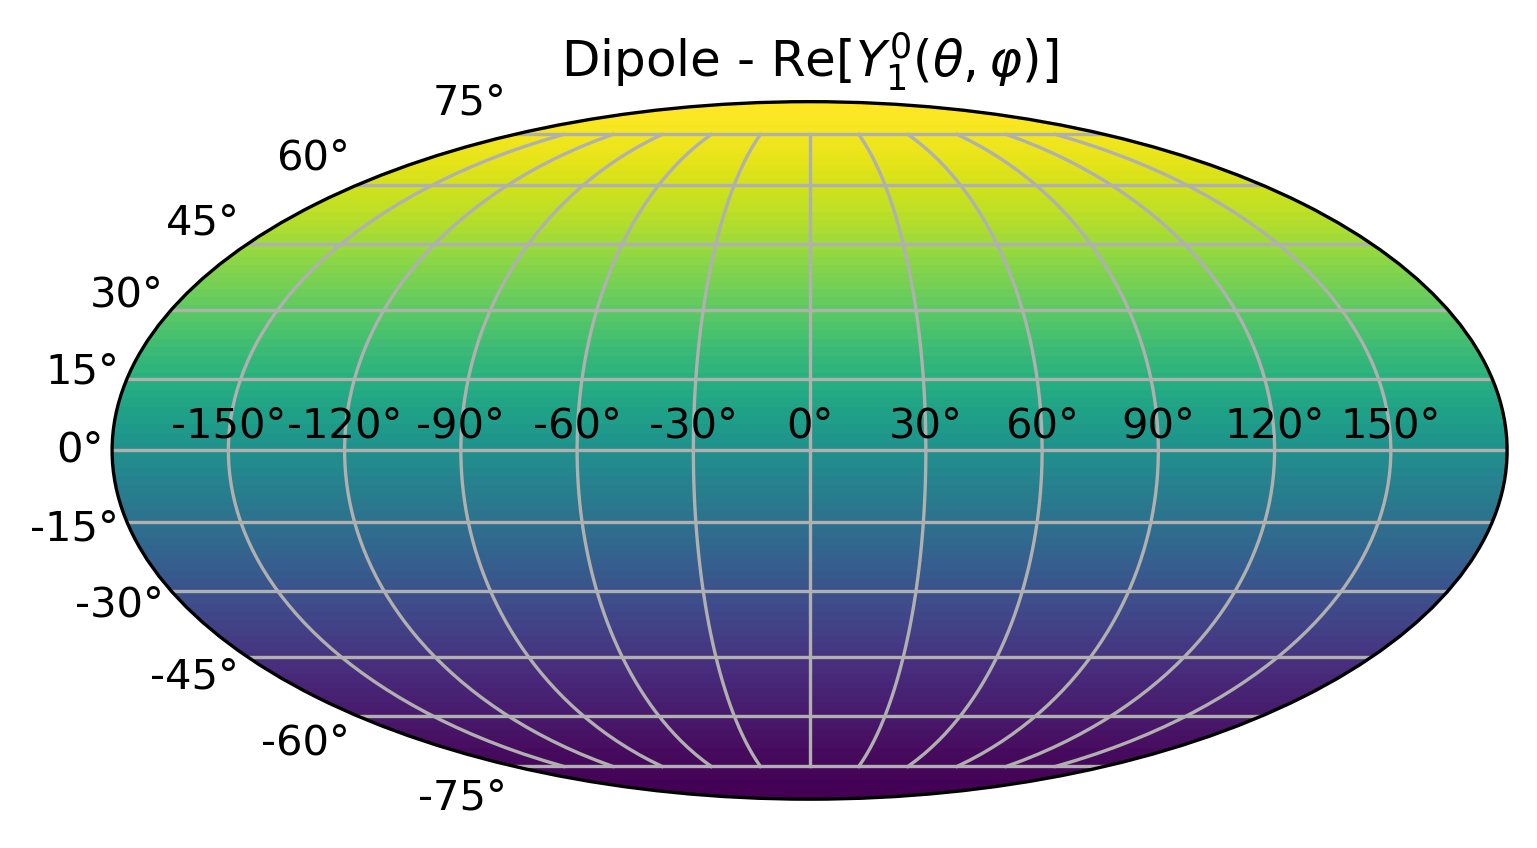
\includegraphics[width=\textwidth]{Sph Harm Examples/dipole Y01.png}
    \caption{}
    \label{subfig: dipole example 01}
  \end{subfigure}
  \begin{subfigure}[b]{0.3\textwidth}
    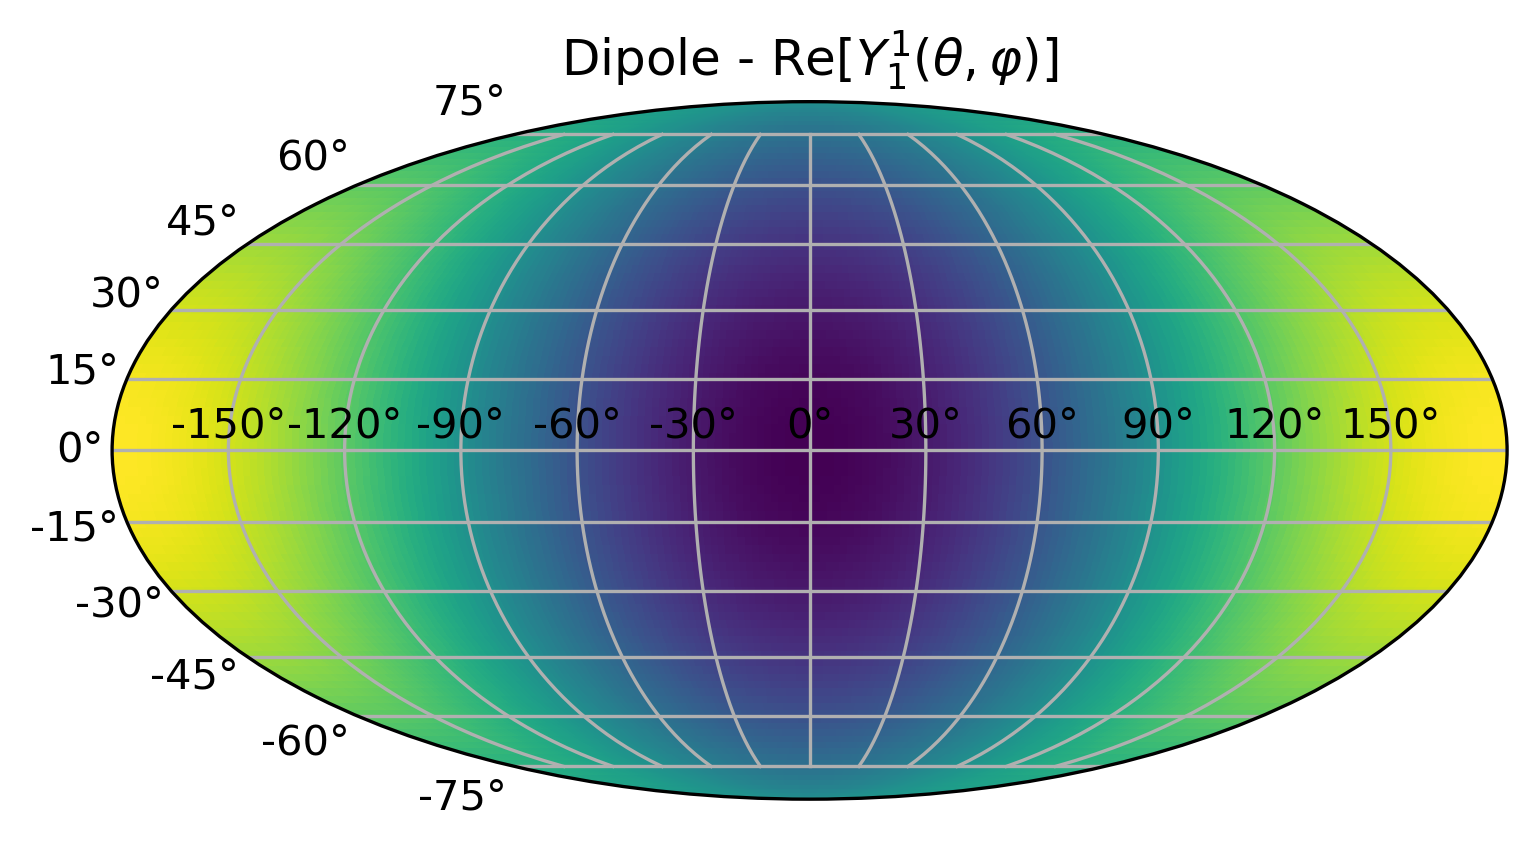
\includegraphics[width=\textwidth]{Sph Harm Examples/dipole Y11 Re.png}
    \caption{}
    \label{subfig: dipole example 11}
  \end{subfigure}
  \\
  \begin{subfigure}[b]{0.3\textwidth}
    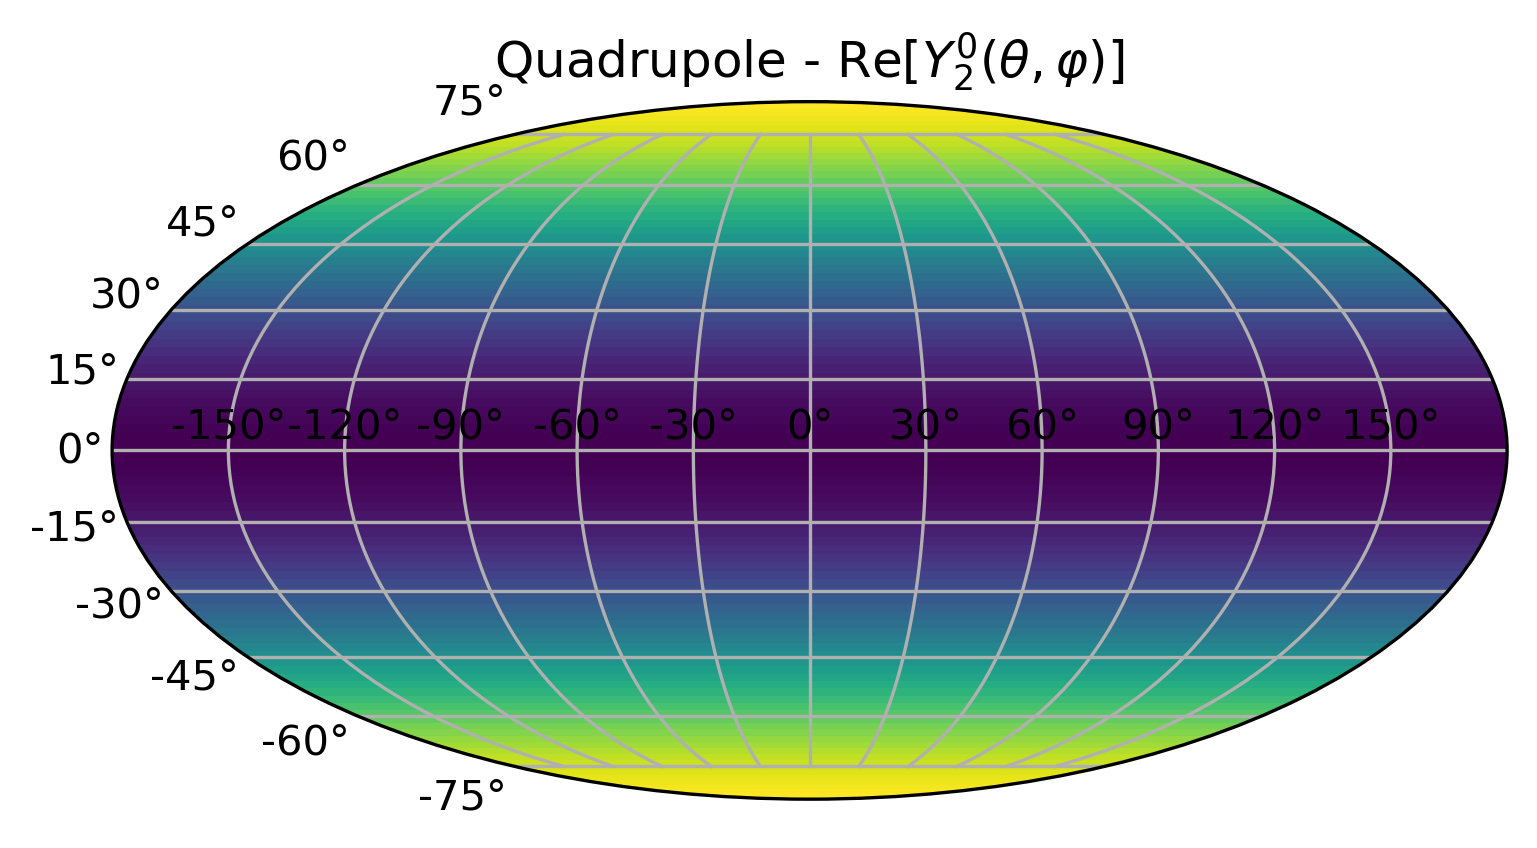
\includegraphics[width=\textwidth]{Sph Harm Examples/Quadrupole Y02.png}
    \caption{}
    \label{subfig: quadrupole example 02}
  \end{subfigure}
  \begin{subfigure}[b]{0.3\textwidth}
    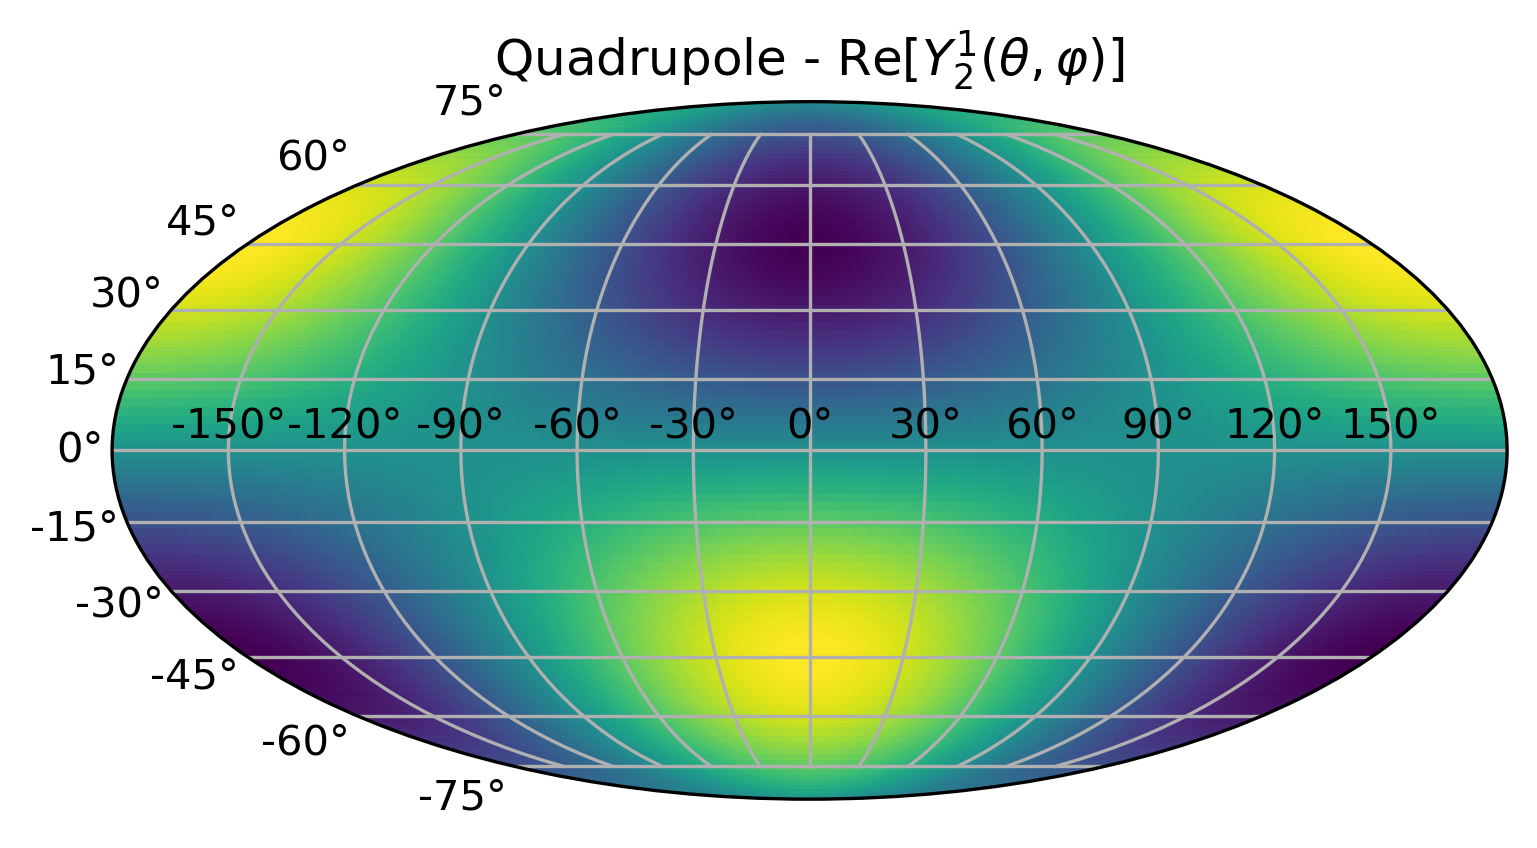
\includegraphics[width=\textwidth]{Sph Harm Examples/Quadrupole Y12 Re.png}
    \caption{}
    \label{subfig: quadrupole example 12}
  \end{subfigure}
  \begin{subfigure}[b]{0.3\textwidth}
    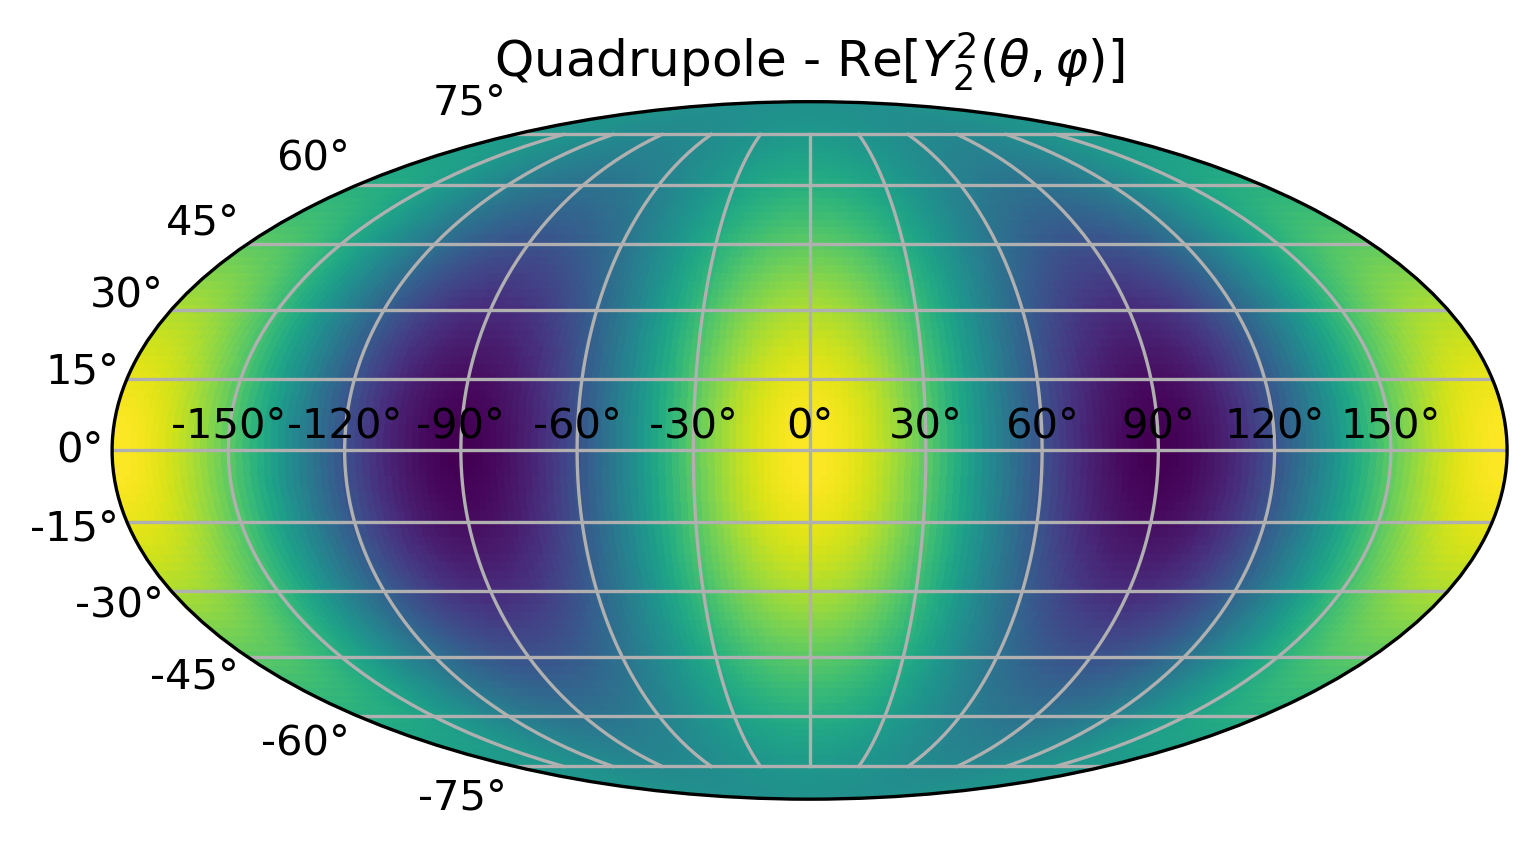
\includegraphics[width=\textwidth]{Sph Harm Examples/Quadrupole Y22 Re.png}
    \caption{}
    \label{subfig: quadrupole example 22}
  \end{subfigure}
  \caption{Examples of purely real dipoles (a, b) and quadrupoles (c, d, e). Plots of function on a sphere throughout this thesis, this figure included, are plotted in a Mollweide projection.}
  \label{fig: Sph Harm Examples}
\end{figure}

When the original function $g$ is purely real, its dipole component can also be written as
\begin{equation} \label{eqn: dipole amplitude definition}
  \sum_{m=-1}^1 a^m_1 Y^m_1 (\theta, \varphi) = \mathcal{D} \cos\phi,
\end{equation}
where $\phi$ is the angular separation between the dipole direction and the point $(\theta, \varphi)$, and $\mathcal{D} \in \mathbb{R}$ is the amplitude of the dipole. We can relate $\mathcal{D}$ to the dipole power $C_1$ as follows: multiply both sides of (\ref{eqn: dipole amplitude definition}) by their complex conjugate,
\begin{equation}
  \left(\sum_{m=-1}^1 a^m_1 Y^m_1\right)\left(\sum_{m'=-1}^1 a^{m'}_l Y^{m'}_1\right)^* = \mathcal{D}^2 \cos^2\phi.
\end{equation}
Expanding and integrating over the sphere gives
\begin{equation}\label{eqn: relation of Cl to D working step}
  \sum_{m=-1}^1 \sum_{m'=-1}^1 a^m_1 (a^{m'}_1)^* \sphint{Y^m_1 (Y^{m'}_1)^*} = \mathcal{D}^2 \sphint{\cos^2\phi}.
\end{equation}
Using the normalisation (\ref{eqn: sph harm normalisation}), the off diagonal elements on the LHS of \eqref{\ref{eqn: relation of Cl to D working step}} vanish, and we get
\begin{equation}
  \sum_{m=-1}^1 |a^m_1|^2 = \mathcal{D}^2 \sphint{\cos^2\phi}.
\end{equation}
We evaluate the integral on the RHS by rotating the coordinates so that $\theta = \phi$, then applying the substitution $u = \cos\theta$
\begin{align*}
   \sphint{\cos^2\phi} &= \sphint{\cos^2\theta}\\
                       &= \int_{\varphi=0}^{2\pi}  \int_{\theta=0}^\pi \cos^2\theta \sin\theta \diff{\theta} \diff{\varphi}\\
                       &= 2\pi \int_{\theta=0}^\pi \cos^2\theta \sin\theta \diff{\theta}\\
                       &= 2\pi \int_{u=-1}^{1} u^2 \diff{u}\\
                       &= \frac{4\pi}{3}
\end{align*}
\begin{equation}
  \Longrightarrow\sum_{m=-1}^1 |a^m_1|^2 = \frac{4\pi}{3} \mathcal{D}^2
\end{equation}
Finally, this rearranges to
\begin{equation} \label{eqn: dipole amplitude from power}
  \mathcal{D} = \sqrt{\frac{3}{4\pi}\sum_{m=-1}^{1}|a^m_1|^2} = \sqrt{\frac{9}{4\pi}C_1}
\end{equation}


%%%%%%%%%%%%%%%%%%%%%%%%%%%%%%%%%%%%%%%%%%%%%%%%%%%%%%%%%%%%%%%%%%%%%%%%%%%%%%%%
%% The Standard Model
\section{The Standard Model of Cosmology}
The standard model of cosmology, also known as the Lambda Cold Dark Matter ($\Lambda$CDM) model or the ``concordance model'', is currently the most widely accepted model of the Universe on its largest scales. With the addition of radiation species (photons and neutrinos), it uses Einstein's theory of General Relativity to describe the Universe from very early times onwards. The name $\Lambda$CDM comes from the model's use of a cosmological constant $\Lambda$ modelling the dark energy that drives the expansion of the Universe, and the inclusion of nonbaryonic cold dark matter (CDM) which does not interact electromagnetically and is modelled as a pressureless dust.

%% The Cosmological Principle
\subsection{The Cosmological Principle and Large Scale Structure}
Underpinning the standard model of cosmology is the \textit{Cosmological Principle}. This assumption states that on large enough scales, the Universe appears to be spatially homogeneous and isotropic. More specifically, there is a set of spacelike hypersurfaces $\Sigma_t$ understood as hypersurfaces of constant cosmic time, and when the density field on each hypersurface is averaged on scales larger than the scale of statistical homogeneity it appears homogeneous and isotropic. This principle was implicit in Einstein's first cosmological models \cite{RN44}, and first discussed by Milne \cite{RN43}.

Observationally, the Cosmological Principle is supported by the high degree of isotropy seen in the Cosmic Microwave Background (CMB). After the large dipole anisotropy has been subtracted, the remaining anisotropies are generally at the level of $|\Delta T/T|\leq 10^{-5}$ \cite{RN54}. The large dipole component is normally interpreted as solely due to our motion with respect to the hypersurfaces of average homogeneity $\Sigma_t$. We will examine the CMB and its dipole in greater depth later on in this chapter. The Cosmological Principle is supported also by the almost isotropic distribution of galaxies at large distances in the sky. However, there are contradictory measurements regarding this \cite{RN151,RN51,RN152,RN52,RN53,RN202,RN49,RN50}.

On scales of tens of megaparsecs, the Universe is very inhomogeneous. Galaxies are arranged in filaments and sheets which thread and surround large cosmic voids. These voids are make up $\sim 40\%$ of the volume of the Universe at low redshift, have an average diameter of about $30 h^{-1} \mathrm{Mpc}$\footnote{Here and throughout the thesis we use units $h^{-1} \text{Mpc}$ for distance. These are units defined such that $H_0 = 100\, h\, \si{km.s^{-1}.Mpc^{-1}}$.}, and a density contrast of $\delta_\rho = (\rho-\bar{\rho})/\bar{\rho} < -0.9$ \cite{RN149,RN150}, where $\rho$ is the mass density and $\bar{\rho}$ is the average mass density. This arrangement forms the cosmic web \cite{RN55,RN56,RN59}.

\subsubsection{The Scale of Statistical Homogeneity}
\newcommand{\domtoavg}{{\mathcal{D}_R}}
\newcommand{\domtoavgcust}[1]{{\mathcal{D}_{#1}}}
\newcommand{\avgdensity}{\langle \rho(t) \rangle_{\domtoavg}}
On larger scales, we would expect to see the average homogeneity and isotropy assumed by the Cosmological Principle. Generally, one deals with averages in a domain $\domtoavg$ contained in a surface of constant time $\Sigma_t$ \cite{RN147},
\begin{equation}\label{eqn: example density average}
    \langle \rho(t) \rangle_{\domtoavg} = \frac{1}{\mathcal{V}(t)}\int_\domtoavg \rho(t,\vec{x}) \sqrt{\text{det}\,^3g} \diff{^3 \vec{x}}
\end{equation}
where $\mathcal{V}(t)$ is the volume of the $\domtoavg$, given by
\begin{equation}
    \mathcal{V}(t) \equiv \alpha R(t)^3 = \int_\domtoavg \sqrt{\text{det}\,^3g} \diff{^3 \vec{x}}.
\end{equation}
In this form $R$ acts like the radius of the domain, with $\alpha$ being a dimensionless constant depending on the geometry. For example, in a Euclidean space where $\domtoavg$ is a sphere, $\alpha = 4\pi/3$. Using averages such as \eqref{\ref{eqn: example density average}}, one can define scales of homogeneity. One approach is to assume the ergodic hypothesis -- this originates from the statistical physics of isolated systems; we treat galaxy positions as a realisation of a random distribution and assume that averaging over many disjoint regions of the same scale is representative of an ensemble average of the underlying distribution on that scale \cite{RN177} -- and to presuppose an average positive density $\rho_0(t)$ defined by
\begin{equation}
    \lim_{R\to\infty} \avgdensity = \rho_0(t) > 0.
\end{equation}
Then a homogeneity scale, $\lambda_0(t)$, can be defined \cite{RN257} by the requirement that for all $R > \lambda_0$ each point in $\Sigma_t$ is contained in a domain $\domtoavgcust{\lambda_0} \subset \domtoavg$ such that $\left|\avgdensity-\rho_0(t)\right| < \rho_0(t)$ \cite{RN201}.

Practically, the density field must be inferred from galaxy catalogues, which are subject to finite sample volumes and observational biases. Taking these issues into account, galaxy-galaxy correlation functions are used in studies of the homogeneity scale. The two point correlation function $\xi(\Delta)$ is the excess probability\footnote{Here, excess probability is the probability in excess of what one would get if galaxies were independently and randomly distributed with a uniform probability.} of finding a galaxy at a distance of $\Delta$ from another Galaxy. The three point correlation function is the excess probability of finding three galaxies with specified distances between each other. The excess probability of finding $N$ galaxies separated by specified distances is the $N$-point correlation function \cite{RN118}. In a statistically homogeneous universe, we would expect all the $N$-point galaxy correlation functions to go to zero as the scale of distances examined increases.

Using Newtonian N-body simulations, an approximate upper bound on the scale of statistical homogeneity of $260\,h^{-1}\,$Mpc is expected in the $\Lambda$CDM cosmology \cite{RN152}, and when only considering the two-point correlation function one observes emergence of homogeneity as low as $70 - 120 \, h^{-1}\,$Mpc \cite{RN52,RN53}. However, current observations suggest that when considering all $N$-point correlation functions, one can infer that the scale of statistical homogeneity must be beyond $700\, h^{-1}\,$Mpc, if it exists at all \cite{RN202}. This along with the observation of abnormally large structures -- such as a large quasar group of characteristic size $\sim 500\,$Mpc and longest dimension $\sim1240\,$Mpc \cite{RN49}, and the recent discovery of a `Giant Arc on the Sky' which has a characteristic length of $\sim 1\,$Gpc \cite{RN225} -- challenge the scales at which statistical homogeneity is usually assumed.

\subsubsection{Coarse-Graining and Backreaction}
If one assumes the Cosmological Principle, then the approach of the standard model of cosmology is to model the Universe as described above as an FLRW geometry above the scale of statistical homogeneity. The FLRW geometry is an exact solution of Einstein's equations with a natural notion of a cosmic rest frame which forms the spatial hypersurfaces $\Sigma_t$, on which the metric possesses 6 Killing vectors corresponding to maximal spatial symmetry (isotropy and homogeneity). However, from a viewpoint of fundamental General Relativity, the Cosmological Principle and use of the FLRW metric is an ansatz that needs to be verified, and given the above difficulties with finding the scale of statistical homogeneity, it is also troublesome observationally.

General Relativity is very well verified on a stellar scale by the dynamics of planets, stars, and black holes. But on larger scales, we need to `fit' or average these stellar scale dynamics into larger geometries if we wish to describe these larger scale systems using General Relativity. This is known as the `fitting problem' \cite{RN203,RN204,RN179}.

Solving the `fitting problem' to find the average dynamics of the Universe on its largest scales will require coarse-graining: averaging and smoothing over the fine detail to obtain a simplified model of the Universe on a larger scale. This coarse-graining can be schematically represented as the following hierarchy \cite{RN179}:
\begin{equation}\label{eqn: averaging schematic}
\left.
\begin{array}{r}
    g^\text{stellar}_{\mu\nu} \to g^\text{galaxy}_{\mu\nu} \to g^\text{cluster}_{\mu\nu} \to g^\text{wall}_{\mu\nu} \\
    \vdots \\
    g^\text{void}_{\mu\nu}
\end{array}
\right\}
\to g^\text{universe}_{\mu\nu}.
\end{equation}
The geometry and dynamics of stars are coarse-grained to get the geometry and dynamics of galaxies. Galaxies are then coarse-grained up to galaxy clusters, which are then coarse-grained up to the thin galactic filaments and walls. Finally, these structures are coarse grained in all their different types along with cosmic voids to get the coarse-grained geometry and dynamics of the Universe.

Coarse-graining is well understood for non-gravitational degrees of freedom. The inner dynamics of stars and planets can be ignored, and they can be treated as point particles. Unfortunately, gravitational energy cannot be localised. One can obtain many notions of quasilocal gravitational energy, but none of these are unique \cite{RN205}. Additionally, there is no unique way to integrate tensors to obtain an average. Consequently, there are many different ways to approach coarse-graining. The three most prominent approaches are:
\begin{itemize}
    \item \textit{Scalar Averaging}: In this scheme one makes a foliation of spacetime into spatial hypersurfaces, and then averages the scalars associated with Einstein's equations rather than averaging tensors directly \cite{RN207,RN208}. More recently, a generalised formalism has been derived, leading to a natural class of proper time foliations and a minimal number of backreaction terms \cite{RN206}.
    \item \textit{Macroscopic Gravity}: In this scheme Zalaletdinov \cite{RN211,RN209,RN210} introduces additional mathematical structure, bitensors, which act as a tensor at each point, but a scalar when defining an integral on a region of spacetime. The formalism is designed to work between two levels of a coarse-graining hierarchy, such as those in \eqref{\ref{eqn: averaging schematic}}, assuming general covariance at each level. However, the additional mathematical structure requires many assumptions to apply it to cosmology \cite{RN212,RN213,RN214,RN215}.
    \item \textit{Green-Wald Averaging}: Green and Wald \cite{RN216} use a scheme aimed at examining the effects of small-scale inhomogeneities on the averaged large scale Universe. This scheme assumes that spacetime is described by a single parameter family of metrics, which can be split into a background and its deformations. The metric evolves by Einstein's equations with an effective fluid, though not necessarily a perfect fluid, and the energy-momentum tensor may be different to the background one. Green and Wald have shown that within this scheme, backreaction -- which is defined in a way specific to their scheme -- is negligible \cite{RN216,RN217,RN218}. However, this scheme is narrower in what it can be applied to, so these conclusions do not apply to other schemes such as scalar averaging \cite{RN153,RN219}.
\end{itemize}
In scalar averaging, the averaged dynamics do not in general coincide with Einstein's equations for an effective average matter fluid. The evolution equations can be written in a form which resembles the Friedmann equation (\ref{eqn: Friedmann Equation 1}), however, additional terms arise due to the effects of the inhomogeneity which have been averaged over. These terms are backreaction terms, and if the FLRW model is sufficient to describe the Universe on some large scale, we might expect the backreaction terms to vanish at that scale. However, there are alternative proposals in which backreaction makes significant enough a contribution that not only is the evolution non-FLRW, but dark energy is potentially not required. While backreaction terms themselves may only contribute at the percent level, the contribution of spatial curvature -- which no longer scales in the manner of an FLRW model -- is generally found to dominate in viable scenarios \cite{RN226,RN227,RN154,RN229,RN230,RN231}.

So despite underlying the greatly successful standard $\Lambda$CDM model, the modern era of precision cosmology has revealed the Cosmological Principle may be at odds with the observed Universe, and from a theoretical standpoint there is no widely accepted justification for the Cosmological Principle. For a more in depth review of this topic, see \cite{RN194}.


%% The FLRW Metric
\subsection{The Friedmann-Lemaître-Robinson-Walker Metric}
In the standard $\Lambda$CDM model, the Friedmann-Lemaître-Robinson-Walker (FLRW) metric describes the geometry of the Universe above the scale of statistical homogeneity. It results from assuming invariance of the geometry under spatial translations and rotations as per the Cosmological Principle. In comoving coordinates with units where $c=1$, it is
\begin{equation}\label{eqn: FLRW metric}
  ds^2 = -\diff{t}^2 + a^2(t)\left[\frac{1}{1-kr^2}\diff{r}^2 + r^2\left(\diff{\theta}^2+\sin^2(\theta)\diff{\phi}^2\right)\right],
\end{equation}
where $k=-1,0,1$ is the spatial curvature, corresponding to hyperbolic, flat, or spherical geometry respectively, and $a(t)$ is the cosmic scale factor. The expansion of the Universe is determined by the change in $a(t)$, and is commonly described with the following parameters,
\begin{align}
  H(t) &\equiv \frac{\dot{a}}{a},\\
  q(t) &\equiv \frac{-\ddot{a}}{aH^2},\\
  j(t) &\equiv \frac{1}{aH^3}\deriv{^3 a}{t^3},
\end{align}
where $\dot{}=\deriv{}{t}$ is the derivative with respect to the coordinate time (also called cosmic time). These parameters are the Hubble parameter, the deceleration parameter, and the jerk parameter respectively. The values of these parameters at the present epoch $t=t_0$ is represented by a subscript zero, for example, the Hubble constant is $H_0 = H(t_0) = 100\, h\, \si{km.s^{-1}.Mpc^{-1}}$.

In $\Lambda$CDM, the energy momentum tensor is assumed to take the form of a perfect fluid,
\begin{equation}\label{eqn: FLRW energy momentum tensor}
  T^{\mu \nu} = (\rho + P)U^{\mu}U^{\nu}+Pg^{\mu \nu},
\end{equation}
where $\rho$ is the local mass-energy density of the fluid, $P$ is the pressure of the fluid, related to $\rho$ by an equation of state $P=w\rho$, and $U^\mu = \delta^\mu_t$ is the 4-velocity of the congruence of comoving particles in the fluid. The sources of energy are:
\begin{itemize}
  \item Radiation (denoted with subscript $r$): such as photons and high energy particles, with $w=1/3$;
  \item Pressureless dust (denoted with subscript $m$): representing baryonic matter and cold dark matter, with $w=0$.
\end{itemize}
Additionally, the cosmological constant $\Lambda$ in Einstein's equations can alternatively be re-expressed as a perfect fluid with constant density $\rho_\Lambda = \Lambda/(8\pi G)$ and $w=-1$. Other possible sources of energy such as cosmic string gas with $w=-1/3$ or stiff matter with $w=1$ are sometimes included, but these are not relevant to this thesis, so will not be discussed.

The modelling of the matter as dust on large scales is somewhat problematic conceptually. A pressureless dust consists of many identical particles of constant mass which interact with each other only gravitationally, which above a certain scale can be treated as an averaged fluid element. However, there are no particles which clearly fit this definition, and averaging procedures have struggled to justify the use of the FLRW metric within theory. The largest identifiable ``particles'', or bound structures, are galaxy clusters. However, these are not homogeneously distributed. We have to average on scales larger than the largest typical structures ($\sim30\,h^{-1}\,$Mpc diameter voids) to obtain a fluid element whose mass does change over the time scale of the evolution problem in question. Despite this, the FLRW model combined with perturbation theory or Newtonian N-body simulations fits most features and observations of the Universe on its largest scale. For a more in depth discussion of the use of dust and the averaging problem, see Wiltshire (2011) \cite{RN179}.

The Einstein equations for the FLRW metric with energy momentum tensor (\ref{eqn: FLRW energy momentum tensor}) give the Friedmann equation,
\begin{equation}\label{eqn: Friedmann Equation 1}
  3\frac{\dot{a}^2}{a^2}=8\pi G \rho - 3\frac{k}{a^2} + \Lambda,
\end{equation}
and the acceleration equation
\begin{equation}\label{eqn: acceleration equation}
  3\frac{\ddot{a}}{a} = \Lambda - 4\pi G \left(\rho + 3P\right).
\end{equation}
The equation of energy-momentum conservation $\nabla^\mu T_{\mu\nu}=0$ gives
\begin{equation}\label{eqn: FLRW energy-momentum conservation}
  \dot\rho + 3\frac{\dot{a}}{a}(\rho + P) = 0.
\end{equation}
In the above three equations $\rho$ gives the total mass-energy density (excluding that contributed by the cosmological constant).
Note that these three evolution equations are not independent, by using the Bianchi identity, \eqref{\ref{eqn: acceleration equation}} can be derived from \eqref{\ref{eqn: Friedmann Equation 1}} and \eqref{\ref{eqn: FLRW energy-momentum conservation}}. The dynamics of $\Lambda$CDM are commonly rewritten using the following density parameters,
\begin{align}
  \Omega_m(t) &= \frac{\rho_m}{\rho_c} = \frac{8\pi G\rho_m}{3H^2},\\
  \Omega_k(t) &= \frac{-k}{a^2 H^2}, \\
  \Omega_\Lambda(t) &= \frac{\rho_\Lambda}{\rho_c} = \frac{\Lambda}{3H^2},
\end{align}
where $\rho_c(t)=3H^2 / 8\pi G$ is the critical density parameter. This is the density of a spatially flat universe consisting only of pressureless dust ($k=0$, $\Lambda=0$, $P=0$). It demarcates $\Lambda=0$ solutions which expand forever (open universes, $k=-1$) from those that eventually recollapse (closed universes, $k=1$). Using the density parameters, the Friedmann equation can be written as
\begin{equation}
  \Omega_m + \Omega_r + \Omega_\Lambda + \Omega_k = 1.
\end{equation}

The Planck collaboration \cite{RN32} infers the present values of the $\Lambda$CDM parameters from CMB measurements as
\begin{align}
  \Omega_{m0}&\equiv\Omega_m(t_0) = 0.3111 \pm 0.0056 \\
  \Omega_{\Lambda 0}&\equiv\Omega_\Lambda(t_0) = 0.6889 \pm 0.0056 \\
  \Omega_{k0}&\equiv\Omega_k(t_0) = 0.0007 \pm 0.0019 \\
   H_0 &= 67.66 \pm 0.42\, \si{km.s^{-1}.Mpc^{-1}}.
\end{align}
Observations suggest that the present radiation density is very small, having a value around $\Omega_r (t_0) \sim 10^{-4}$. Since this and the spatial curvature $\Omega_k$ both take up a very small amount of the total energy budget, they are both usually neglected.

Within the standard $\Lambda$CDM model, the FLRW metric is normally paired with perturbation theory, Newtonian N-body simulations, and bulk flows to model structures below the scale of statistical homogeneity. However, within this thesis, we will use exact inhomogeneous solutions of Einstein's equations to model structure. To see how this approach compares to perturbation theory, see \cite{RN6}.


%% Redshifts and Distances
\subsection{Cosmological Redshift and Distances}
Using the standard $\Lambda$CDM model, we can calculate observables to check the consistency of the model and analyse data. The most relevant of these to this thesis are the luminosity distance $d_L$, angular distance $d_A$, and redshift parameter $z$ of light sources such as stars and galaxies.

The redshift parameter $z$ is the fractional change in wavelength of an observed photon as compared to its wavelength at the source. It is defined as
\begin{equation}
  z \equiv \frac{\lambda_{obs}-\lambda_{em}}{\lambda_{em}},
\end{equation}
where $\lambda_{obs}$ is the wavelength of the photon as measured by the observer, and $\lambda_{em}$ is the wavelength of the photon as measured in the rest frame of the source. Within $\Lambda$CDM, observers are said to be comoving if they are in the rest frame of the dust, (i.e., they have constant spatial coordinates $r,\theta,\phi$). The redshift between two comoving observers in an FLRW metric, one who emits a photon at cosmic time $t_{em}$, and one who receives it at $t_0$, can be obtained by integrating the radial null geodesic between observer and emitter to give,
\begin{equation}\label{eqn: standard model - cosmological redshift}
  (1+z)_{\text{FLRW}}=\frac{a(t_0)}{a(t_{em})}.
\end{equation}
This is known as cosmological redshift. In general, sources and observers will be moving with respect to comoving observers, so the observed redshift will be
\begin{equation} \label{eqn: standard model - redshift with doppler}
  1+z = (1+z)_{\text{FLRW}} (1+z)_{\text{Doppler}}.
\end{equation}
The Doppler factor includes effects of the local boosts of the observer and the source. This difference in velocity with respect to comoving observers also creates aberration, a change in the direction of the photon towards the direction of motion, as measured by the observer. With a decomposition of the observed redshift assuming a cosmic rest frame as per \eqref{\ref{eqn: standard model - redshift with doppler}}, the effects of aberration can be determined purely from special relativity. If we neglect the motion of the source, then we only need to transform the photon's 4-momentum measured at the location of the observer in the cosmic rest frame, $p^{\mu} = E(1,-\uvec{n})$, to that measured in the observer's boosted frame $p^{\mu'}=E'(1,-\uvec{n}')$, where $\uvec{n}$ and $\uvec{n}'$ are outward pointing unit 3-vectors aligned with the direction in the sky that we see the photon originating from in the comoving and boosted observer's frames respectively. A minus sign is applied to incoming photons, as these unit vectors are in the opposite direction to the movement of the photon. The factors $E$ and $E'$ are the energies of the photon as measured in each frame. We apply a Lorentz boost as follows,
\begin{equation} \label{eqn: SR boost - lorentz boost of 4-momentum}
  p^{\mu'} = \Lambda^{\mu'}_\nu p^\nu,
\end{equation}
where $\Lambda^{\mu'}_\nu = \partial x^{\mu'} / \partial x^\nu$ is the Jacobian matrix for the change of basis vectors under a Lorentz boost. Its components are
\begin{equation}\label{eqn: SR boost - lorentz boost matrix}
  (\Lambda^\mu_\nu) = \begin{bmatrix}
    \gamma              & -\gamma\bm{\beta}^\intercal \\
    -\gamma\bm{\beta}   & I_3 + (\gamma - 1)\uvec{\beta}\uvec{\beta}^\intercal
\end{bmatrix}.
\end{equation}
Here $I_3$ is the $3 \times 3$ identity matrix, $\bm{\beta}=(\beta_x,\beta_y,\beta_z)^\intercal$ is the 3-velocity of the boost, $\beta=|\bm{\beta}|$ is the boost parameter, $\uvec{\beta} = \bm{\beta}/\beta$ is the unit vector in the direction of the boost, and $\gamma=(1-\beta^2)^{-1/2}$ is the Lorentz factor. Taking the time component of (\ref{eqn: SR boost - lorentz boost of 4-momentum}) describes the redshift effect,
\begin{align}\label{eqn: SR boost - redshift}
  \nu'&=\gamma(1+\bm{\beta}\cdot\uvec{n})\nu.
\end{align}
When this is applied to a frequency distribution, such as the light coming from a blackbody via the Planck relation $E=h\nu$, this causes the distribution to appear hotter in the direction of motion and cooler in the opposite direction. This effect is known as the modulation of the temperature.

Taking the spacelike component of (\ref{eqn: SR boost - lorentz boost of 4-momentum}) describes the aberration effect,
\begin{align}\label{eqn: SR boost - aberration}
  \hat{\bm{n}}' = \frac{\hat{\bm{n}}+\left[\gamma\beta+(\gamma - 1)\uvec{\beta}\cdot\uvec{n}\right]\uvec{\beta}}{\gamma(1+\bm{\beta}\cdot\uvec{n})}.
\end{align}
We can manipulate Eqs.~(\ref{eqn: SR boost - redshift}) and (\ref{eqn: SR boost - aberration}) to obtain the following formula for the Doppler redshift factor, written in terms of the more convenient $\uvec{n}'$ instead of $\uvec{n}$:
\begin{equation}\label{eqn: SR boost - redshift factor}
  (1+z)_{\text{Doppler}} = \gamma (1-\bm{\beta}\cdot\hat{\bm{n}}').
\end{equation}


The radial coordinate $r$ used in the FLRW metric is not directly measurable. A more suitable distance measure relating to observation is the luminosity distance $d_L$. For a source of absolute bolometric luminosity $\mathcal{L}$ in its rest frame with flux $\mathcal{F}$ measured by an observer, the luminosity distance measured by the observer is defined as
\begin{equation}
  d_L \equiv \sqrt{\frac{\mathcal{F}}{4\pi\mathcal{L}}}.
\end{equation}
One can relate the cosmological redshift to the luminosity distance by integrating the distance of the radial null interval travelled by the light, and using the Friedmann equation (\ref{eqn: Friedmann Equation 1}), giving,
\begin{equation}
  d_L = \frac{1+z}{H_0 \sqrt{|\Omega_{{k0}}|}}\text{sinn}\left(\sqrt{|\Omega_{{k0}}|} \int_1^{1+z} \frac{dx}{\sqrt{\Omega_{\Lambda 0} + \Omega_{k0}x^2 + \Omega_{m0}x^3 + \Omega_{r0}x^4}}\right),
\end{equation}
where
\begin{equation}
  \text{sinn}(x)\equiv \begin{cases}
    \sin (x), & k=+1 \\
    x, & k=0\\
    \sinh (x), & k=-1
\end{cases}.
\end{equation}
Here $z$ is purely the cosmological redshift between a comoving source and observer. Alternatively, for low redshifts we can express $d_L$ using a Taylor series without reliance on the composition of the energy-momentum tensor \cite{RN220},
\begin{equation} \label{eqn: standard model - d_L Taylor series}
  d_L=\frac{1}{H_0}\left[z + \frac{1}{2}(1-q_0)z^2-\frac{1}{6}(1-q_0-3q_0^2+j_0+\frac{k}{H_0^2 a_0^2})z^3+\mathcal{O}(z^4)\right],
\end{equation}
where again a subscript zero refers to the present value, so $q_0 = q(t_0)$, and $j_0 = j(t_0)$.

Another useful distance measure is the angular diameter distance $d_A$. This is defined as the ratio of the proper diameter of an object $\ell_\theta$, to the angle it subtends in the sky $\delta$,
\begin{equation}
  d_A \equiv \frac{\ell_\theta}{\delta}.
\end{equation}
It is related to the luminosity distance by the reciprocity theorem \cite{RN64,RN102},
\begin{equation}
  d_L = (1+z)_{\text{FLRW}}^2 d_A,
\end{equation}
which in fact applies to any spacetime, not just the homogeneous and isotropic FLRW spacetimes.


%% The Cosmic Microwave Background
\section{The Cosmic Microwave Background}
Using the standard model of cosmology and our understanding of particle physics, the physics of the early universe is well established after the time of the Quark Hadron Transition (at $t \sim 10^{-6} - 10^{-5}\, \si{s}$) Our knowledge of the early universe is constrained by observations such as the relative abundances of light isotopes that arise from primordial nucleosynthesis (\ce{^{1}H}, \ce{^{2}H}, \ce{^{3}He}, \ce{^{4}He}, \ce{^{7}Li}), and experiments in high energy physics such as those undertaken at the Large Hadron Collider. At these early times, the matter of the Universe (referred to as the primordial soup or the primordial plasma) was in a hot and dense equilibrium, with frequent interactions between particles. As the Universe expanded and cooled these interactions became less common, and various particles could condense out of equilibrium, eventually allowing more complex structure to form (such as nuclei, then atoms and molecules, then eventually the stars and galaxies we see today).

As we study earlier epochs, when the average energy density is higher, our understanding of physics eventually approaches regimes which cannot be tested terrestrially, even in the Large Hadron Collider. Before the Quark Hadron Transition, the primordial soup was too hot for neutrons and protons to form, and so consisted of a quark/gluon plasma, the behaviour of which is difficult to probe with our current experimental technology. An early epoch of exponentially fast expansion -- the inflationary universe -- is generally involved. While consistent with observations, such as the spectrum of density fluctuations that generate anisotropies in the CMB, inflation is a phenomenology which may be a hint of a more fundamental theory still to be discovered.

Initially, the primordial soup was opaque to photons due to their frequent interactions with leptons and baryons, resulting in a short mean free path. Once the Universe had expanded and cooled enough, atomic and molecular hydrogen could form. This is known as the era of recombination. At this point, the photons decoupled from the plasma, and could propagate mostly unimpeded. During this period, the Universe can still be treated as being in thermal equilibrium, so this happens at roughly the same time everywhere. The epoch at which the primordial soup was last opaque is idealised as a hypersurface called the surface of last scattering, although of course it has a finite thickness. At the present time, photons originating from the primordial soup can be detected, and have been redshifted by a factor of $z \sim 1100$ to microwave wavelengths. This background radiation is known as the Cosmic Microwave Background (CMB).

The CMB has a near perfect blackbody spectrum with a mean temperature of $2.72548 \pm 0.00057\,$K \cite{RN70}. After subtraction of the dipole component and foreground contributions from the Milky Way and point sources, the spectrum is highly isotropic over the sky with anisotropies on the level of a few parts in 100,000. This is consistent with near homogeneity and thermal equilibrium at the surface of last scattering.

The CMB anisotropies provide extremely valuable information, providing constraints on the initial conditions to structure formation. These anisotropies are divided into two categories:

\subsubsection{Primary Anisotropies}
These anisotropies are caused by the physics of the early universe, originating before the time of recombination. This category includes intrinsic differences in the temperature of the primordial soup, Doppler shifts from variations in the velocity of the primordial soup, and gravitational redshift and blueshift from fluctuations in the gravitational potential at the epoch of last scattering. This last effect is known as the (ordinary) Sachs-Wolfe effect, and is the dominant effect observationally \cite{RN46}.

\subsubsection{Secondary Anisotropies}
These anisotropies are solely due to the effects of structure between the observer and the surface of last scattering. This includes gravitational lensing, the effects of interactions between photons and matter\footnote{This includes the Sunyaez-Zel'dovich effect, where photons undergo inverse Compton scattering with high energy electrons in a galaxy clusters \cite{RN159,RN161}; and the Vishniac effect, where the photons interact with heated gas moving in a bulk motion during the era of galaxy formation \cite{RN162}.}, and the net redshift or blueshift resulting from passing through an overdensity or void.

Speaking relative to the mean cosmic expansion, a photon will be blueshifted when entering an overdensity, and redshifted when exiting the overdensity (and vice versa for an underdensity). The gravitational potential associated with the structure will evolve over time, resulting in the blueshift and redshift not quite cancelling out. The result of many evolving structures as treated with linear perturbation theory on an FLRW background is known as the integrated Sachs-Wolfe effect \cite{RN46}, and the effect from a single large structure in the non-linear regime is known as the Rees-Sciama effect \cite{RN45}.

\subsection{The CMB Dipole}
The dipole component that is subtracted from the CMB is much larger than these primary and secondary anisotropies. When measured in the heliocentric frame, the dipole anisotropy is about one part in 1,000, with an amplitude of \cite{RN71}
\begin{equation} \label{eqn: CMB dipole magnitude}
  \Delta T = 3.3645 \pm 0.0020\, \text{mK}
\end{equation}
in the direction
\begin{equation} \label{eqn: CMB dipole direction}
  (l,b) = (263.99\degree \pm 0.15\degree, 48.26\degree \pm 0.03\degree).
\end{equation}
The galactic coordinates $l$ and $b$ are angular coordinates on the celestial sphere with the sun as its centre, aligned so that $(l,b)=(0\degree,0\degree)$ is directed at the approximate centre of the Milky Way, and the equator $b=0\degree$ is parallel to an approximation of the galactic plane. Much like traditional latitude and longitude, galactic latitude $b \in [-90\degree, 90\degree]$ gives the angle northward of the galactic equator, and the galactic longitude $l \in (-180\degree, 180\degree]$ is the angular distance along the galactic equator eastward of the Galactic Centre.

\subsubsection{The Kinematic Dipole Interpretation}
The large dipole is normally assumed to be purely the result of the motion of the heliocentric frame relative to the frame in which the CMB is most uniform, called the CMB rest frame. The motion causes modulation and aberration as per Eqs.~(\ref{eqn: SR boost - redshift}) and (\ref{eqn: SR boost - aberration}). The blackbody spectrum as measured in the CMB rest frame in direction $\uvec{n}$ with measured temperature $T(\uvec{n})$ is boosted to a blackbody spectrum with temperature in the direction $\uvec{n}'$ given by
\begin{equation} \label{eqn: SR boost - temperature redshift}
  T'(\uvec{n}') = \frac{T(\uvec{n})}{\gamma(1-\bm{\beta}\cdot\uvec{n}')}.
\end{equation}
Assuming a small boost parameter $\beta$ we can apply a Taylor expansion to (\ref{eqn: SR boost - temperature redshift}) to obtain
\begin{equation}
  T'(\uvec{n}') = T(\uvec{n})\left(1+\bm{\beta}\cdot\uvec{n}'+(\bm{\beta}\cdot\uvec{n}')^2-\frac{1}{2}\beta^2+\mathcal{O}(\beta^3)\right).
\end{equation}
In the simple case of an isotropic temperature $T(\uvec{n})=T_0=2.72548\,$K, we see that the first order effect of the boost is a dipole component
\begin{equation}
  T'(\uvec{n}') = T_0(1+\bm{\beta}\cdot\uvec{n}' + \mathcal{O}(\beta^2)).
\end{equation}
The CMB photons coming in from the direction of motion are blueshifted, and the CMB photons coming in from the opposite side are redshifted. This is known as a kinematic dipole. It is standard practice to assume that other effects are negligible and that the CMB dipole is purely kinematic. This gives the velocity of the heliocentric frame relative to the CMB rest frame as $369.82 \pm 0.11 \,\text{km s}^{-1}$, or $\beta = (1.23357 \pm 0.00036)\times 10^{-3}$ \cite{RN32}.

Recent studies have shown that the CMB dipole may have a significant non-kinematic component \cite{RN35,RN40,RN3,RN34,RN33,RN31,RN68,RN167}, for example, due to a non-negligible differential expansion. This hypothesis is the focus of this thesis.

\subsection{The Angular Power Spectrum of the CMB}
When analysing CMB data using the power spectrum, what is conventionally of interest instead of $C_\ell$ is
\begin{equation} \label{eqn: sph harm D_l definition}
  \mathcal{D}_\ell = \frac{\ell(\ell+1)C_\ell}{2\pi} \langle T \rangle_\Omega^2,
\end{equation}
where $C_\ell$ refers to the power spectrum of $\Delta T / \langle T \rangle_\Omega$, and $\langle T \rangle_\Omega$ is the average temperature over the whole sky.

This statistic is used because the observed CMB power spectrum takes the form $C_\ell \sim \frac{2\pi}{\ell(\ell+1)}$ when the fluctuations in the primordial soup are scale-invariant, as is predicted by inflationary paradigms. This is quantified by the spectral index of the primordial fluctuations taking the value $n_s = 1$ \cite{RN177}. The 2018 Planck measurements show that $n_s$ is very close to $1$, deviating slightly to $n_s = 0.9652 \pm  0.0042$ \cite{RN176}. Figure \ref{fig: Planck CMB power spectrum} shows $D_\ell$ as determined from the 2018 Planck data and its best fit to the standard $\Lambda$CDM model.

\begin{figure}[t]
  \centering
  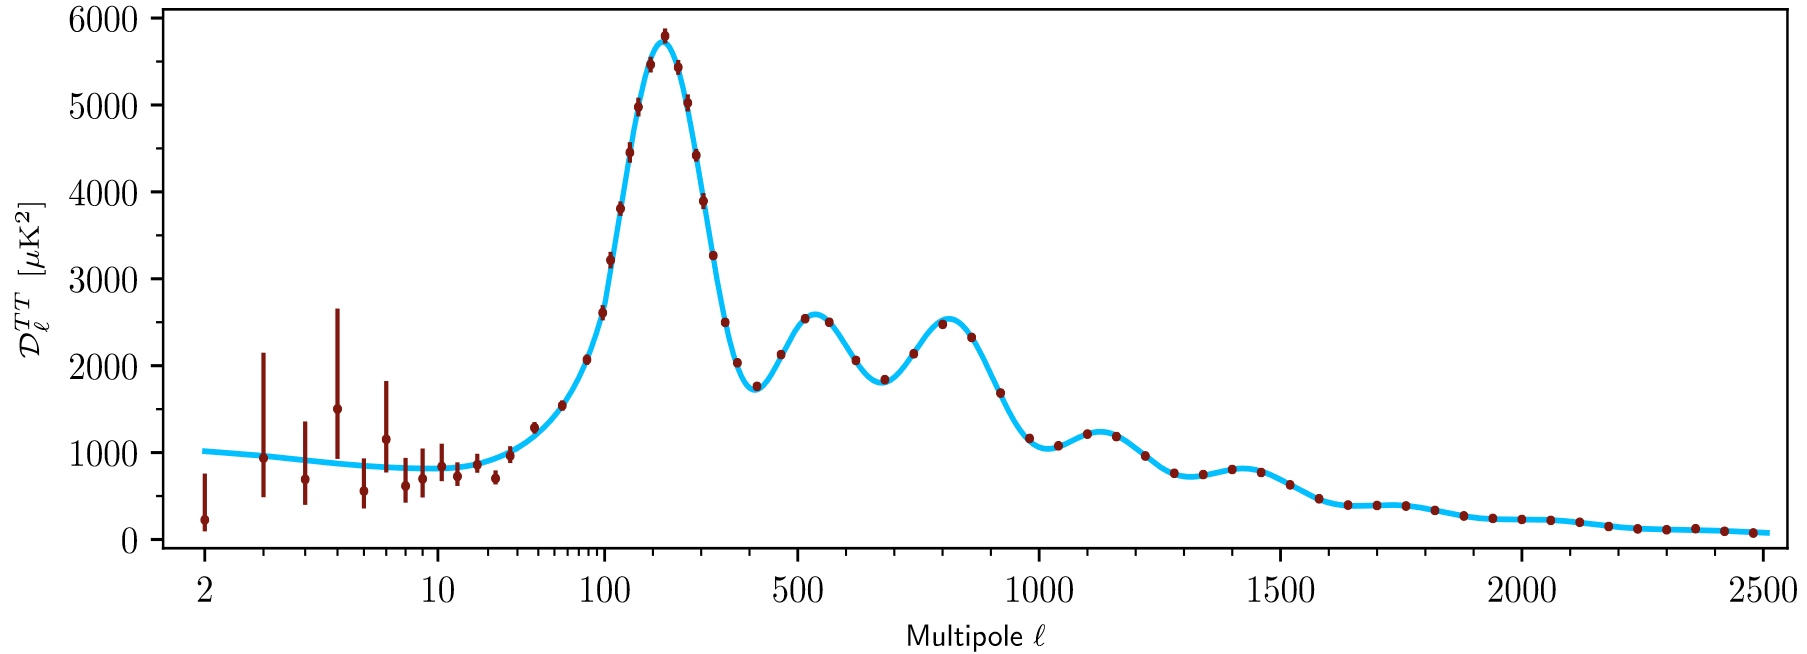
\includegraphics[width=0.9\textwidth]{Planck CMB Power Spectrum TT.png}
  \caption{The CMB temperature power spectrum for $\ell \geq 2$ from the 2018 Planck data. The blue curve shows the best-fitting $\Lambda$CDM model. Figure Credit: Planck Collaboration 2018 \cite{RN32}}
  \label{fig: Planck CMB power spectrum}
\end{figure}

The peaks seen in the power spectrum are caused by sound waves in the primordial plasma, supported by the pressure of electromagnetic interactions. While the dark matter density contributes the largest component to the overall density, being pressureless it does not form standing waves but clumps gravitationally even in the early universe. Electromagnetically charged particles -- dominated in mass by baryons given the small electron to proton mass ratio of $1/1897$ -- are prevented from clumping by the pressure. At last scattering, the reionization of hydrogen and helium causes this pressure support to cease, and the acoustic oscillations are `frozen in' \cite{RN221}. The acoustic oscillations can be decomposed into sine waves across various scales. As sine waves spend more time at their maxima, when the oscillations are `frozen in' there will be an excess of density perturbations corresponding to an oscillation which has undergone one rarefaction or one compression. The wavelength of this will be equal to the \textit{sound horizon}: the furthest distance a sound wave can travel by the time of last scattering \cite{RN176}. The excess in power of density perturbations at this wavelength affects the redshift of light due to the Sachs-Wolfe effect, causing an increase in angular power in the observed CMB temperature differences at an angular scale known as the Baryon Acoustic Oscillation (BAO) scale \cite{RN222}. This can be seen as the dominant peak in the plot of the angular power of the CMB temperature, seen in Figure \ref{fig: Planck CMB power spectrum} \cite{RN176,RN223}. Sound waves which have time to undergo one rarefaction and one compression by the time of last scattering form the second peak in the same way. Sound waves which have undergone a rarefaction, compression, then a rarefaction (or a compression, rarefaction, then a compression) form the third peak, and likewise for smaller wavelengths \cite{RN224}.

Of particular interest to this thesis is the observed quadrupole ($\ell=2$), which has a power much lower than expected from the $\Lambda$CDM model. The observed quadrupole only has a power of \cite{RN175}
\begin{equation}
  \mathcal{D}_2 = 225.9^{+533.1}_{-132.4}\, (\mu\si{K)^2},
\end{equation}
which can be seen in Figure \ref{fig: Planck CMB power spectrum}. From this, we can assume that any contribution from local structure to the quadrupole must be negligible.

%%%%%%%%%%%%%%%%%%%%%%%%%%%%%%%%%%%%%%%%%%%%%%%%%%%%%%%%%%%%%%%%%%%%%%%%%%%%%%%%
\section{Redshift in Generic Cosmic Expansion}\label{section: generic redshift}
The observables of interest in this thesis (CMB measurements and galaxy catalogues) are made are by observing light (visible or otherwise). In a general geometry, the observed redshift of a photon is
\begin{equation}\label{eqn: general redshift}
    1+z_\text{obs} = \frac{\left. U^{\hat{a}}_\text{em} k_{\hat{a}}\right| _{\vec{x}_1}}{\left. U^{\hat{b}}_\text{obs} k_{\hat{b}}\right|_{\vec{x}_0}},
\end{equation}
where $k^{\hat{a}}$ is the tangent vector to the null geodesic -- which could be taken as the 4-momentum or wavenumber 4-vector of the photon as desired -- in the Lorentz frame of the observer at $\vec{x}_0$ or the the emitter at the earlier $\vec{x}_1$. The vectors $U_\text{obs}^{\hat{a}}$ and $U_\text{em}^{\hat{a}}$ are the 4-velocities of the observer and emitter respectively, again in their local Lorentz frame.

While the concept of velocity as a local boost in the tangent space at a point is always well defined, any extension to a relation describing galaxies separated by tens or hundreds of megaparsecs is merely an ansatz. For the purposes of classifying the redshift in an exact solution of Einstein's equations with the metric $g_{\mu\nu}$, we choose ideal model observers at $\vec{x}_0$ and $\vec{x}_1$ with 4-velocities $U_0^\mu$ and $U_1^\mu$ respectively, and include the effects of Lorentz transforms to their frames to re-express \eqref{\ref{eqn: general redshift}} as
\begin{equation}\label{eqn: general redshift peculiar split}
    1+z_\text{obs} = \frac{\left. U^\mu_0 k_\mu\right| _{\vec{x}_0}}{\left. U^{\hat{a}}_\text{obs} k_{\hat{a}}\right|_{\vec{x}_0}}\,
    \frac{\left. U^\nu_1 k_\nu\right| _{\vec{x}_1}}{\left. U^\sigma_0 k_\sigma\right|_{\vec{x}_0}}\,
    \frac{\left. U^{\hat{m}}_\text{em} k_{\hat{m}}\right|_{\vec{x}_1}}{\left. U^\rho_1 k_\rho\right|_{\vec{x}_1}}.
\end{equation}
We denote the first and last factors of the right side $(1+z_{\text{pec},0})$ and $(1+z_{\text{pec},1})$ respectively, which are the peculiar velocity corrections from the Lorentz transformation. The two ideal model observers are somewhat arbitrary, but in dust solutions of Einsteins equations the natural choice is the observer comoving with the dust. Evaluating the redshift now requires parallel propagating the invariant $U^\nu_1 k_\nu$ from the emitter to the observer along the null geodesic with initial tangent vector $k^\mu |_{\vec{x}_1}$.

In equation \eqref{\ref{eqn: general redshift peculiar split}}, the middle term is evaluated in the coordinate frame. If the coordinates are chosen so that the ideal model observers are at rest in both locations, $U_0^i = U_1^i = 0$, then \eqref{\ref{eqn: general redshift peculiar split}} can be expressed as
\begin{align}
    1+z_\text{obs} &= (1+z_{\text{pec},0})\,
    \frac{\left. g_{tt} U^t_1 k^t\right| _{\vec{x}_1}}{\left. g_{tt} U^t_0 k^t\right|_{\vec{x}_0}}\,
    (1+z_{\text{pec},1}), \\
    &= (1+z_{\text{pec},0})\,
    (1+z_\text{cos})\,
    (1+z_{\text{pec},1})
\end{align}

We can further split the cosmological expansion term as
\begin{equation}
    1+z_\text{cos} \equiv
    \frac{\left. g_{tt} U^t_1 k^t\right| _{\vec{x}_1}}{\left. g_{tt} U^t_0 k^t\right|_{\vec{x}_0}} =
    (1+z_{\phi,0})(1+\bar{z})(1+z_{\phi,1}),
\end{equation}
with
\begin{align}
    1+z_{\phi,0}
    = \left. \frac{1}{-g_{tt}U_0^t}\right|_{\vec{x}_0}
    = \frac{1}{\sqrt{-g_{tt}(\vec{x}_0)}}, \\
    1+z_{\phi,1}
    = \left. \frac{1}{-g_{tt}U_1^t}\right|_{\vec{x}_1}
    = \frac{1}{\sqrt{-g_{tt}(\vec{x}_1)}},
\end{align}
interpreted as ``gravitational redshift'' relative to the ``background expansion''
\begin{equation}
    1+\bar{z} = \frac{k^t(\vec{x}_1)}{k^t(\vec{x}_0)}.
\end{equation}

With these definitions, we can re-express the observed redshift as
\begin{equation} \label{eqn: generic redshift factors}
    1+z_\text{obs} = (1+z_{\text{pec},0})
    (1+z_{\phi,0})(1+\bar{z})(1+z_{\phi,1})
    (1+z_{\text{pec},1}).
\end{equation}
Observationally, the split into these different factors is ambiguous, since there is no clear choice of the ideal model observers. Even if we assume the CMB dipole is purely kinematic, that only gives the first term. If additionally one has a model of the average background redshift (e.g., assuming a background FLRW geometry, or using an average model with backreaction), the split between the source's gravitational redshift $(1+z_{\phi,1})$ and its peculiar velocity redshift $(1+z_{\text{pec},1})$ is ambiguous without making additional model assumptions.

In the standard model, one takes the average expansion $1+\bar{z}$ to be that of an FLRW model, and assumes the gravitational potential terms are small, $|z_{\phi,0}| \ll 1$ and $|z_{\phi,1}| \ll 1$, so that they can be treated with perturbation theory in the linear regime and numerical simulations in the non-linear regime.

%%%%%%%%%%%%%%%%%%%%%%%%%%%%%%%%%%%%%%%%%%%%%%%%%%%%%%%%%%%%%%%%%%%%%%%%%%%%%%%%
%% Galaxy Surveys
\section{Galaxy Catalogue Studies}\label{section: galaxy catalogue studies}
Galaxy catalogues provide us with a way to test the standard $\Lambda$CDM model as constrained by CMB measurements, assuming we have a sufficiently accurate understanding of the luminosity and frequency distribution of radiation from distant radio galaxies and quasars. Points of concern from such studies relevant to this thesis are the observations of a large scale bulk flow beyond standard $\Lambda$CDM model predictions (typically from Newtonian N-body simulations), and the kinematic cosmic dipole tension.

\subsection{Bulk Flows}\label{section: bulk flows}
Within the framework of the standard $\Lambda$CDM model, we expect the observed redshift-distance relation to slightly differ from \eqref{\ref{eqn: standard model - d_L Taylor series}} due to perturbations from the FLRW background. These are normally treated with perturbation theory and Newtonian N-body simulations. As per \eqref{\ref{eqn: standard model - redshift with doppler}}, these perturbations can be interpreted as velocities with respect to the `cosmic rest frame'. Thus we define the \textit{peculiar velocity} as the velocity a galaxy would have as observed in this frame.
For small redshifts, we see from (\ref{eqn: standard model - d_L Taylor series}) that the cosmological redshift obeys a linear relation
\begin{equation}
  z_\text{cos} = H_0 d_L.
\end{equation}
Light from an observed source will also have Doppler redshift, $z_\text{Doppler}$, due to the peculiar velocity of the source. Assuming a small cosmological and Doppler redshift, and that redshift from other sources (such as local gravitational redshift) is negligible, the redshift measured by a comoving observer is
\begin{align}
    \begin{split}\label{eqn: obs redshift linear breakdown}
        z_\text{obs} &= (1+z_\text{Doppler})(1+z_\text{cos}) - 1 \\
        &\approx z_\text{Doppler} + z_\text{cos} \\
        &\approx v_{\text{pec}, \parallel} + H_0 d_L,
    \end{split}
\end{align}
where $v_{\text{pec}, \parallel}$ is the component of the peculiar velocity away from us. Thus from an observation of a source's redshift and luminosity distance, we can infer the component of the peculiar velocity away from us to be approximately
\begin{equation} \label{eqn: peculiar velocity from linear distance-redshift}
  v_{\text{pec}, \parallel} = z_\text{obs} - H_0 d_L,
\end{equation}
where $z_\text{obs}$ and $d_L$ are taken in the `cosmic rest frame'. Supernovae measurements are usually taken in a geocentric or heliocentric frame, assuming a kinematic CMB dipole it is trivial to convert to the `cosmic rest frame'. However, the validity of \eqref{\ref{eqn: peculiar velocity from linear distance-redshift}} relies on the observed redshift taking the form in \eqref{\ref{eqn: obs redshift linear breakdown}}. In general, gravitational redshift from the surrounding environments of both the source and observer and from any structures lying in the way of the light ray will also contribute to the observed redshift. When considering a large catalogue of sources, one might expect the gravitational redshift from the observer's surroundings to have a systematic effect on the observed redshift \cite{RN232}. \eqref{\ref{eqn: peculiar velocity from linear distance-redshift}} is commonly used in combination with the \textit{Newtonian velocity addition} approximation, where velocities are assumed to be low so that relative velocities (and redshifts if they are low) combine linearly when changing frame. For example, the velocity of the Earth relative to the FLRW rest frame, $\vec{v}_\text{geo}$, would be
\begin{equation}
    \vec{v}_\text{geo} = \Bigl(\vec{v}_\text{galaxy} + \vec{v}_\text{Sun} + \vec{v}_\text{Earth}\Bigr)\Bigl(1 + \mathcal{O}\left(\frac{v}{c}\right)\Bigr),
\end{equation}
where $\vec{v}_\text{galaxy}$ is the velocity of the Milky Way as observed in the FLRW rest frame, $\vec{v}_\text{Sun}$ is the velocity of Sun as observed in the galaxy's frame, and $\vec{v}_\text{Earth}$ is the velocity of the Earth as observed in the Sun's rest frame.

This definition of peculiar velocity relies heavily on the `cosmic rest frame' present in FLRW geometries. Additionally denoting this quantity as a velocity is somewhat problematic, as from the perspective of General Relativity velocity is a fundamentally local phenomenon defined in the tangent space, and here it is assigned to distant galaxies. It may be better to merely view it as a useful quantity indicating deviation from the FLRW background. One could also view observed `peculiar velocities' as a result of differential expansion, where the rate of expansion differs from region to region. If one uses a Hubble constant $H_0$ fit to data from all directions, differential expansion would be perceived as a peculiar velocity field relative to the mean isotropic expansion. We discuss this possibility more in Section \ref{section: Non-Kinematic Differential Expansion}.

Assuming the kinematic interpretation of the CMB dipole, one would expect from the Cosmological Principle that peculiar velocities of distant objects far beyond the statistical homogeneity scale are randomly and isotropically distributed when observed from the CMB rest frame. On top of this, we can expect some correlation of the velocities of nearby objects due to gravitational attraction. This correlation of velocities of galaxies is known as a \textit{bulk flow}. Using perturbation theory within the standard $\Lambda$CDM model, we expect the observed peculiar velocities on a spatially flat FLRW background relative to a central observer to be \cite{RN118}
\begin{equation}
  \vec{v}(t_0, \vec{r}) = \frac{H_0\Omega_{m0}^{0.55}}{4\pi} \int \delta_m (\vec{r}') \frac{\vec{r}' - \vec{r}}{|\vec{r}' - \vec{r}|^3}\diff{^3 \vec{r'}^3},
\end{equation}
where $\delta_m$ is the density contrast with respect to the FLRW background, and the power of 0.55 on $\Omega_{m0}$ is obtained from fitting to models with a cosmological constant \cite{RN166}. One important conclusion from this analysis is that the observed bulk flows should die off to zero as we observe deeper and deeper into the Universe.

Once we account for the known motions of the Sun within the Milky Way, and of the Milky Way with respect to the Local Group (LG) of galaxies, vector addition of the relevant velocity contributions estimates a nearby bulk flow of galaxies with an average peculiar velocity of \cite{RN74}
\begin{equation}
  635 \pm 38\, \si{km.s^{-1}},
\end{equation}
in the direction
\begin{equation}
  (l,b) = (276.4\degree, 29.3\degree) \pm 3.2\degree.
\end{equation}
Many studies have observed a bulk flow on scales below $100\, h^{-1}$ Mpc that is consistent with the $\Lambda$CDM prediction (e.g., \cite{RN181,RN185,RN117}). However, on scales of $100\, h^{-1}$ Mpc and greater there are some observations of bulk flows exceeding the $\Lambda$CDM expectation \cite{RN82,RN183,RN78,RN186,RN192}.
Notably, Kashlinsky \etal \cite{RN78} find a bulk flow with an amplitude of $600-1000\, \si{km.s^{-1}}$ on scales $\gtrsim 300\, h^{-1}$ Mpc, far exceeding the standard $\Lambda$CDM model prediction for a bulk flow at this distance.
These results are the subject of much discussion and controversy, with other results giving results consistent with the standard $\Lambda$CDM model prediction \cite{RN181,RN182,RN187,RN188,RN189,RN77}.
A bulk flow on these large scales is well beyond the expected scale of statistical homogeneity, it would be difficult to explain using the standard $\Lambda$CDM model. A comparison of various estimations of the bulk flow to the standard $\Lambda$CDM model prediction can be seen in Figure \ref{fig: bulk flow measurements}.

\begin{figure}[t]
  \centering
  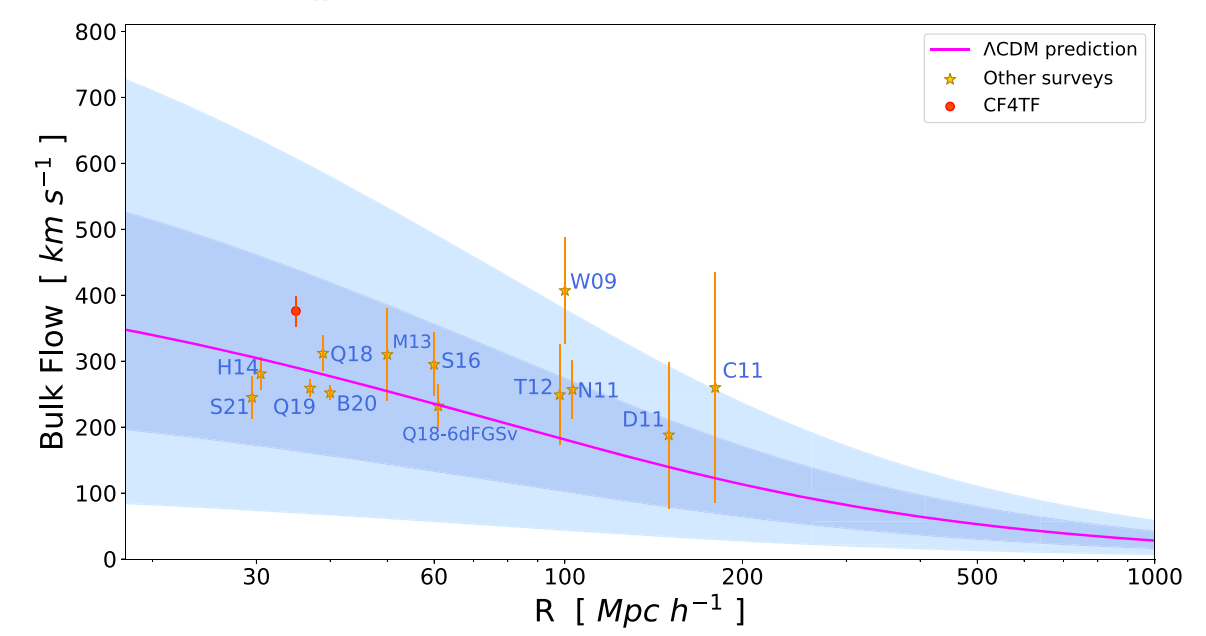
\includegraphics[width=0.8\textwidth]{Bulk Flow Measurements (Qin et al).png}
  \caption{Bulk flow amplitude estimates from various studies as a function of survey depth compared to the standard $\Lambda$CDM model prediction in pink with its $1\sigma$ and $2\sigma$ cosmic variance. Image credit: Qin \etal \cite{RN117}.}
  \label{fig: bulk flow measurements}
\end{figure}

Within the context of perturbations of the standard $\Lambda$CDM model and N-body simulations, one would expect bulk flows (including those consistent with standard $\Lambda$CDM model predictions) to be caused by a distant overdensity gravitationally attracting galaxies\footnote{Despite the common usage of vocabulary such as `attraction' and `infall', the distance between each galaxy and the large distant overdensity actually increases, just at a rate less than expected in a homogeneously expanding universe. This may be viewed as motion on an expanding background as per N-body simulations of the standard $\Lambda$CDM model, or as the expansion rate between the two being less than the global average.}.
The discovery of the Centaurus-Hydra complex (also known as the `Great Attractor') in 1988 at distances of $32 - 60\, h^{-1}\,$Mpc \cite{RN75} was hoped to explain the motion of the Local Group. More recently the Shapely concentration at distances of $120 - 150\, h^{-1}\,$Mpc has been considered. However, there is a lack of expected infall of galaxies on the far side of the concentration, as would be expected from Newtonian N-body simulations \cite{RN77}. So if the bulk flow is due to an attractor, it must be from a structure that is further out.

A recent analysis by Watkins \etal \cite{RN233} of the Cosmicflows-4 galaxy catalogue \cite{RN234} found a bulk flow of magnitude $419 \pm 36\,$km s$^{-1}$ at a survey depth of $200\,h^{-1}\,$Mpc, which is in conflict with the standard $\Lambda$CDM model prediction, with a probability of occurring of only 0.00021\%. Given the lack of evidence for an attractor -- the bulk flows measured in this paper are directed $20\degree$ to $30\degree$ away from the Shapely concentration -- the authors suggest that the observations of anomalously large bulk flows may be due to the particle rest frame of the Universe not being the same as the rest frame inferred from the CMB dipole. This hypothesis also has significant evidence in the distribution of quasars and radio galaxies on the sky, as outlined in the next section.


%% Cosmic Dipole Tension
\subsection{The Kinematic Cosmic Dipole Tension}\label{section: kinematic cosmic dipole tension}
Assuming the standard $\Lambda$CDM model and the kinematic interpretation of the CMB dipole, light coming from on average isotropically distributed distant sources will be subject to only an FLRW cosmological redshift and kinematic effects (relativistic aberration and modulation). We should be able to see the kinematic effects in our observations as creating a dipole in the observed, otherwise isotropic, distribution and fluxes of distant sources. Ellis and Baldwin calculated these effects for populations of distant radio sources \cite{RN67}. To first order in $v/c$, the expected number count per solid angle is
\begin{equation}\label{eqn: E and B galaxy dipole}
  \left(\deriv{N}{\Omega}\right)_{\text{obs}} = \left(\deriv{N}{\Omega}\right)_{\text{rest}}
  \left[1+\left(2+x\left[1+\alpha\right]\right)\frac{v}{c}\cos(\theta)\right],
\end{equation}
where $\theta$ is the angle between the line of sight and the direction of motion, and $\alpha$ is the spectral index of the sources, as populations of distant radio sources are expected to have flux densities following a power law
\begin{equation}
  S(\nu) \propto \nu^{-\alpha},
\end{equation}
and $x$ is similarly related to the population per solid angle with flux above a lower bound $S$,
\begin{equation}
  \deriv{N}{\Omega}(>S) \propto S^{-x},
\end{equation}
as observed in the cosmic rest frame. Assuming kinematic effects dominate, we should observe a dipole in number counts in the same direction as the CMB dipole as per \eqref{\ref{eqn: E and B galaxy dipole}}. Comparison of the observed dipole in catalogues of distant radiation sources (such as radio galaxies or quasars) to \eqref{\ref{eqn: E and B galaxy dipole}} is known as the Ellis-Baldwin test.

The Ellis-Baldwin test has been conducted with a number of radio surveys. However, there increasingly appears to be disagreement between observations and the kinematic expectation. Whether this is a fundamental failure of the Cosmological Principle or a consequence of unaccounted systematic errors and evolutionary effects is a matter of ongoing debate.

Initially, Blake and Wall determined from the NRAO VLA Sky Survey (NVSS) data that the magnitude and direction of the dipole is consistent with the expectation from the CMB dipole \cite{RN88}. However, a reanalysis performed by Singal nine years later using the same data found a dipole that is about 4 times larger than the expectation at the $\sim 3\sigma$ level, despite only a small difference in the method used to determine the dipole \cite{RN90}. This measurement was debated, as the NVSS sample contains many potential sources of systematic error. In 2012, Gibelyou and Huterer \cite{RN171} compared the NVSS dipole to dipole signals from the Two Micron All Sky Survey (2MASS), 2MASS Redshift Survey, and gamma ray bursts in the Burst And Transient Source Experiment, and found that they were all consistent with expectation except the NVSS dipole, which was almost six times as large as expected. Gibelyou and Huterer attributed this to remaining systematic errors in the data. Subsequent studies on the NVSS dipole included the following:
\begin{itemize}
    \item A comparison to the dipole in the Westerbork Northern Sky Survey (WENSS) \cite{RN95,RN170}.
    \item An examination of the dipole in the linearly polarised flux density \cite{RN169}.
    \item Allowance for the behaviour of the number count to deviate from a pure power law \cite{RN172}.
    \item Inclusion of the inhomogeneities expected by $\Lambda$CDM \cite{RN84}.
    \item Inclusion of the Sydney University Molonglo Sky Survey (SUMSS) catalogues to increase sky coverage \cite{RN34}.
\end{itemize}
These investigations disagreed with the expectation from the kinematic CMB dipole, mostly at a level of $\sim 3\sigma$.
The most successful of these at reducing the tension of the NVSS dipole was the paper by Tiwari and Nusser (2016) \cite{RN84} which considered the effect of structure within $\Lambda$CDM. This reduced the disagreement to $2.2 - 2.8\, \sigma$ depending on the method used. But even then, the tension resulting from the NVSS number count dipole still appears significant and resistant to the correction of systematics.

The release of the TIFR GMRT Sky Survey (TGSS) data, carried out by the Giant Metrewave Radio Telescope (GMRT) of the Tata Institute of Fundamental Research (TIFR) \cite{RN92}, gave another independent radio galaxy catalogue to investigate at a lower frequency than NVSS. (TGSS was measured at 150 MHz whereas NVSS was measured at 1.4 GHz.) Studies of the dipole by Bengaly \etal (2018) \cite{RN85} and Singal (2019) \cite{RN33} showed that the amplitude of the number count dipole in TGSS data is even more at odds with the expectation, being $\sim 5$ times larger than the kinematic expectation from the CMB dipole and $\sim 2.5$ times larger than the NVSS number count dipole. Additionally, the TGSS data number count possessed anomalously large angular power for $2 \leq \ell \leq 30$ \cite{RN85,RN174}. This can affect the measured dipole amplitude, but not at a level large enough to fully explain the large dipole. Therefore, systematic errors were initially suspected.

It was subsequently suggested by Siewert \etal in 2021 \cite{RN86} that there may be a frequency dependence of the number count dipole in radio galaxy catalogues. By analysing the dipole from TGSS, WENSS, SUMSS, and NVSS, they found that as the frequency that the survey was taken at increased, the number count dipole decreased. However, this conclusion is very dependent on the TGSS result. Removing it allows a constant dipole amplitude fit over frequency. If the frequency dependence result is found to be significant, it would rule out the kinematic interpretation of these dipoles, as the effect of Lorentz boosts on survey data should be almost frequency independent.

\begin{figure}[t]
  \centering
  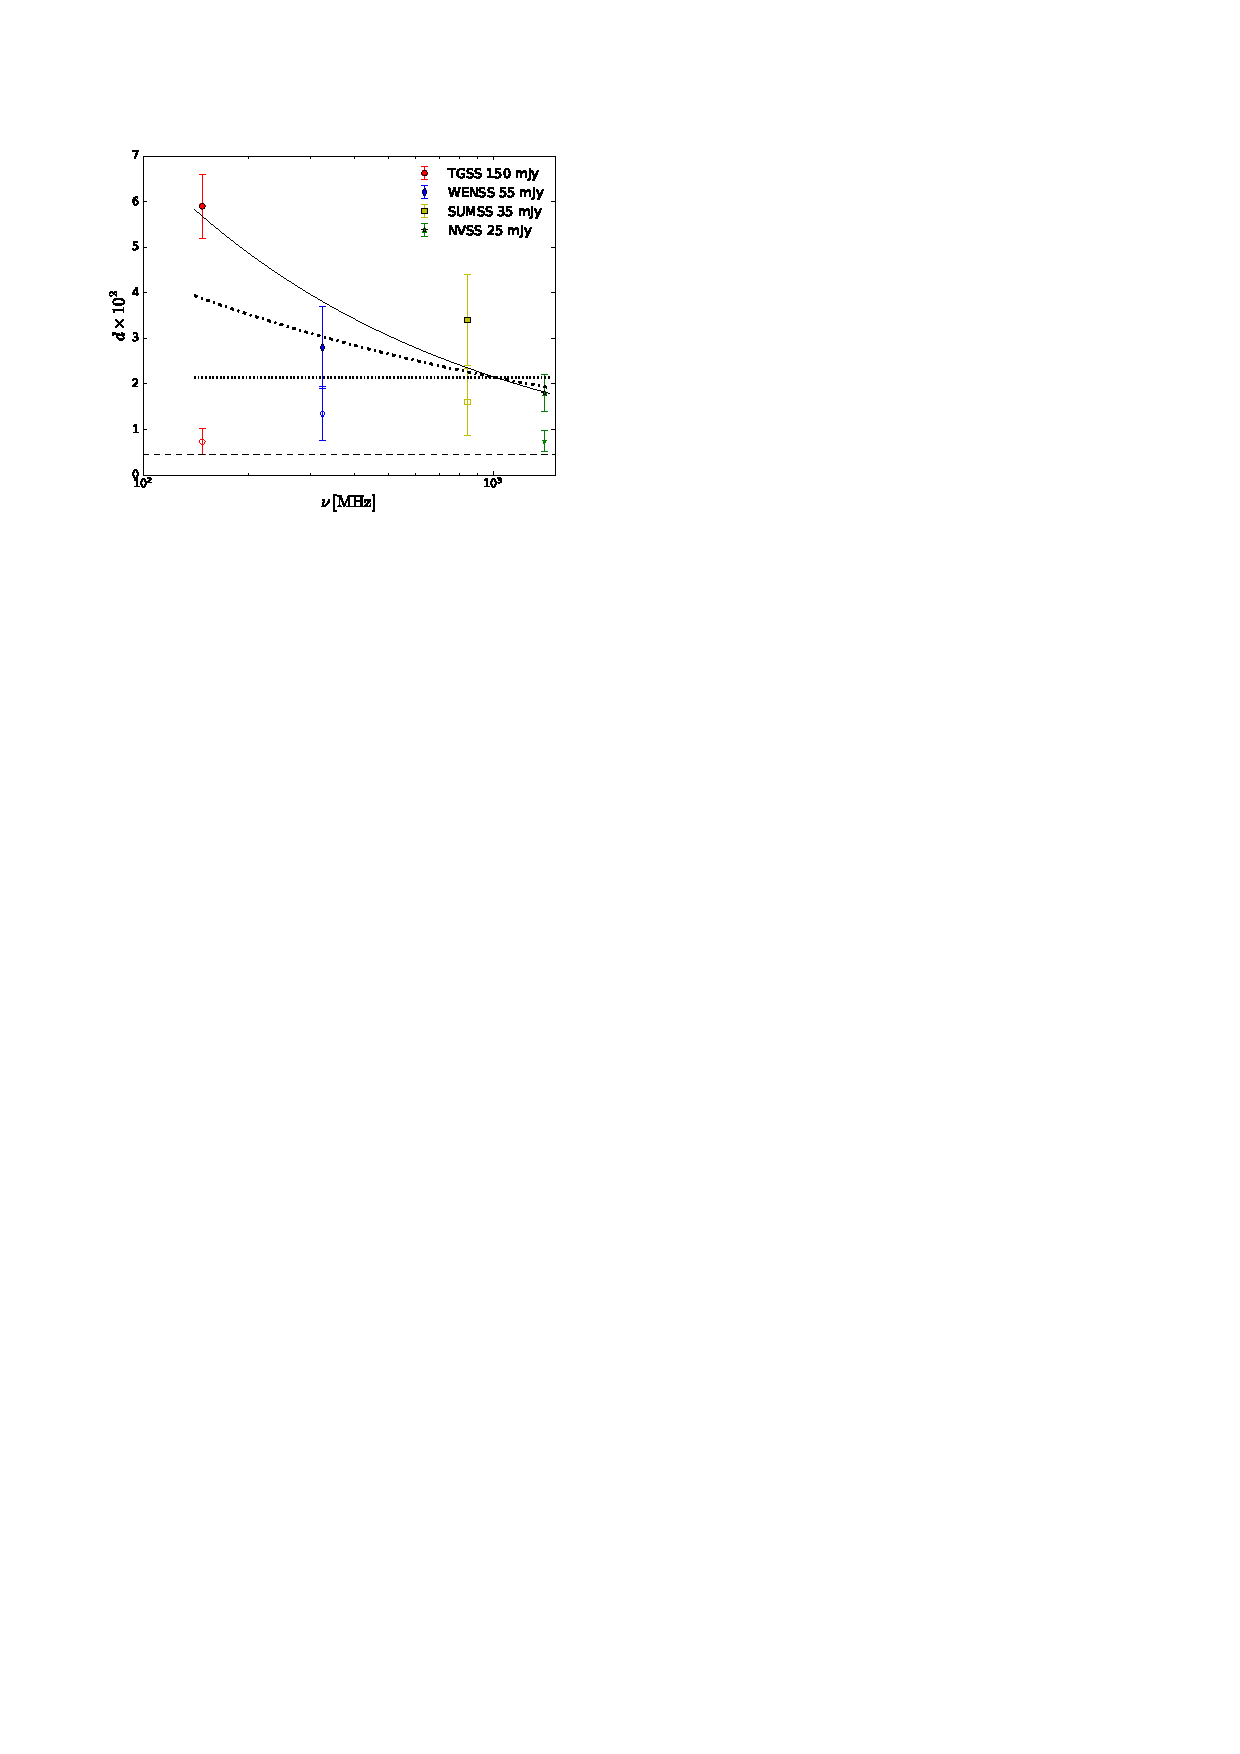
\includegraphics[width=0.6\textwidth]{Siewert 2021 Dipole Frequency Dependence.pdf}
  \caption{Comparison of the amplitude of the number count dipoles as determined using TGSS, WENSS, SUMSS, and NVSS. Solid markers are the observed amplitude, hollow markers are from simulations taking into account the coverage of each survey. The lines from top to bottom as taken at the left of the figure are as follows: the best power law fit for all surveys, the best power law fit excluding TGSS, a constant dipole fit excluding TGSS, and the expectation purely from the measured CMB dipole using \eqref{\ref{eqn: E and B galaxy dipole}}. Figure credit: Siewert \etal (2021) \cite{RN86}.}
  \label{fig: Cosmic Radio Dipole Frequency Dependence from Siewert et al}
\end{figure}

Another independent survey is provided by the CatWISE2020 catalogue \cite{RN91}, from which Secrest \etal (2021) \cite{RN31} created a sample of 1.36 million distant quasars (up to $z \sim 3.5$). They then used this sample to conduct the Ellis-Baldwin test. CatWISE2020 is taken from the Wide-field Infrared Survey Explorer (WISE), a space mission, thus it is not subject to observational systematics that plague ground based surveys, such as atmospheric effects and declination limits. They found a number dipole over twice as large as expected and pointing in a direction $27.8\degree$ from the CMB dipole, initially determined to reject the kinematic CMB dipole at $4.8 \sigma$.
Following this paper, it was suggested by Dalang and Bovin that evolution effects of $\alpha$ and $x$ could bring this significance down to $1-2\sigma$ \cite{RN68}. Just last year, Secrest \etal (2022) \cite{RN167} combined the CatWISE2020 quasar sample with NVSS, improving the significance to $5.1 \sigma$ and finding no evidence of the evolutionary effects suggested by Dalang and Bonvin. Additionally, this paper refutes the frequency dependence suggested by Siewert \etal (2021) \cite{RN86}, finding that when known systematics are accounted for, the number count dipole in TGSS drops by a factor of $\sim 3$ to a level consistent with the number count dipoles found in the WENSS, SUMSS, and NVSS catalogues.

These results suggest that the radio galaxy and quasar count dipoles are not merely the result of systematic errors, perhaps instead originating from incorrectly identifying these dipoles as purely due to kinematics (including the CMB dipoles), or originating from a violation of the Cosmological Principle. Most of the number count and flux dipoles measured are aligned (or close to aligned) with the CMB dipole, which is expected if the dipoles are purely due to kinematic effects. However, if the dipoles have another cause, it also needs to explain this alignment.
We note that catalogues of closer sources (such as 2MASS, which is a catalogue of sources in the infrared rather than radio) are affected by the galaxy clustering of large scale structure, so will naturally disagree with the results from more distant radio galaxies in the NVSS data \cite{RN171,RN125,RN173}.

\begin{table}
  \centering
  \resizebox{\textwidth}{!}{
  \begin{tabular}{l c|c c|r}
    Observation & Catalogue & Apex  & $\mathcal{D}$ & Reference \\
    \hline \hline
    Quasar Dipole (Number Counts) & CatWISE2020 \cite{RN91} & $(l, b) = (238.2, 28.8)\degree$ & $0.01554$ & Secrest \etal (2021) \cite{RN31} \\
    Radio Galaxy Dipole (Number Counts) & TGSS \cite{RN92} & $(l, b) = (243.00 \pm 12.00, 45.00 \pm 3.00)\degree$ & $0.070 \pm 0.004$ & Bengaly \etal (2018) \cite{RN85} \\
    Radio Galaxy Dipole (Number Counts) & NVSS \cite{RN93} & $(l, b) = (253.13 \pm 11.00, 27.28 \pm 3.00)\degree$ & $0.023 \pm 0.04$ & Bengaly \etal (2018) \cite{RN85} \\
    Radio Galaxy Dipole (Number Counts) & NVSS & $(\text{RA}, \text{dec}) = (154 \pm 19, -2 \pm 19)\degree$ & $0.018 \pm 0.006$ & Rubart \& Schwarz (2013) \cite{RN95} \\
    Radio Galaxy Dipole (Number Counts) & WENSS \cite{RN104} & $\text{RA} = (117 \pm 40)\degree$ & $0.029 \pm 0.019$ & Rubart \& Schwarz (2013) \cite{RN95} \\
    Radio Galaxy Dipole (Sky Brightness) & TGSS & $(\text{RA}, \text{dec})=(172 \pm 10, -5 \pm 9)\degree$ & $0.0524 \pm 0.0053$ & Singal (2019) \cite{RN33} \\
    Radio Galaxy Dipole (Number Counts) & TGSS & $(\text{RA}, \text{dec})=(162 \pm 9, 3 \pm 8)\degree$ & $0.0442 \pm 0.0037$ & Singal (2019) \cite{RN33} \\
    Radio Galaxy Dipole (Number Counts) & TGSS & $(\text{RA}, \text{dec})=(140 \pm 11, 13 \pm 11)\degree$ & $0.059 \pm 0.007$ & Siewert \etal (2021) \cite{RN86} \\
    Radio Galaxy Dipole (Number Counts) & WENSS & $(\text{RA}, \text{dec})=(128 \pm 29, -11 \pm 7)\degree$ & $0.028 \pm 0.009$ & Siewert \etal (2021) \cite{RN86} \\
    Radio Galaxy Dipole (Number Counts) & SUMSS & $(\text{RA}, \text{dec})=(108 \pm 23, -4 \pm 9)\degree$ & $0.034 \pm 0.01$ & Siewert \etal (2021) \cite{RN86} \\
    Radio Galaxy Dipole (Number Counts) & NVSS & $(\text{RA}, \text{dec})=(140 \pm 14, -5 \pm 13)\degree$ & $0.018 \pm 0.004$ & Siewert \etal (2021) \cite{RN86} \\
    \hline
    Expected Number Count Dipole from CMB & Radio Galaxy Catalogues &
      \begin{tabular}{@{}c@{}} $(\text{RA}, \text{dec})=(167.9, -6.944)\degree$ \\
      $(l,b) = (264.0, 48.23)\degree$\end{tabular} &
      $0.0046$ &
      Siewert \etal (2021) \cite{RN86} \\
    Expected Number Count Dipole from CMB & CatWISE2020 &
      \begin{tabular}{@{}c@{}} $(\text{RA}, \text{dec})=(167.9, -6.944)\degree$ \\
      $(l,b) = (264.0, 48.23)\degree$\end{tabular} &
      $0.0073$ &
      Secrest \etal (2022)
  \end{tabular}}
  \caption{Amplitude and directions of observed dipoles. The declination for the number count dipole of WENSS in the fifth row is missing as it cannot be determined using the method used in \cite{RN95}. Additionally, a 2021 paper by Siewert \etal \cite{RN86} calculates the dipole with a variety of surveys, masks, and flux density thresholds. All of which show a larger dipole than expected from the kinematic interpretation and in roughly the direction of the CMB dipole.}\label{table: Dipole Measurements}
\end{table}


%%%%%%%%%%%%%%%%%%%%%%%%%%%%%%%%%%%%%%%%%%%%%%%%%%%%%%%%%%%%%%%%%%%%%%%%%%%%%%%%
%% Differential Expansion
\section{Non-Kinematic Differential Expansion}\label{section: Non-Kinematic Differential Expansion}
In the standard $\Lambda$CDM model, we assume an FLRW metric which has a single uniform expansion rate. However, in general since matter and geometry are coupled by Einstein's equations on small scales, the expansion rate can vary due to inhomogeneities. This appears in exact inhomogeneous dust solutions of Einstein's equations such as the Szekeres solutions and LTB solutions, which we discuss in Chapter \ref{chapter: Szekeres Solutions}. Several observational tensions with the standard $\Lambda$CDM model, such as the kinematic cosmic dipole tension or the Hubble tension, may potentially be eased or even resolved if one reconsiders the observations of the CMB and galaxy surveys from first principles with this in mind. Perhaps an approach other than the standard methodology of Section \ref{section: galaxy catalogue studies} would be more appealing.

Given the ambiguity in separating kinematic and gravitational redshifts in generic cosmologies as per \eqref{\ref{eqn: generic redshift factors}}, for scales below the scale of statistical homogeneity but above the scale of gravitationally bound structures, it may make more sense to consider the redshift as the result of varying regional expansion histories. Inhomogeneities may thus give rise to \textit{relativistic differential expansion}, corresponding to gradients in the local expansion of voids and overdensities of large scale structure.

From a catalogue of galaxy redshifts and distances (assuming the catalogue has sufficient coverage), one can determine the local Lorentz frame of \textit{Average Isotropic Expansion} (AIE) as the frame in which a spherically averaged distance-redshift law has minimal variation from a linear Hubble law \cite{RN35,RN40,RN122}. The isotropy in this frame is only an average, so the observed redshift may display nonkinematic effects depending on the direction of the incoming photons, $z\AIE = z\AIE(\uvec{n}\AIE)$.

Bolejko, Nazer, and Wiltshire \cite{RN3} suggest defining \textit{nonkinematic relativistic differential expansion} as occuring when measurements of the CMB in the heliocentric frame give a temperature difference
\begin{equation}\label{eqn: non kinematic relativistic differential expansion BNW definition}
  \Delta T_{\text{nk}-\text{hel}} = \frac{T\AIE}{\gamma\AIE(1-\vec{\beta}\AIE \cdot \uvec{n}_\text{hel})}-
  \frac{T_0}{\gamma\CMB(1-\vec{\beta}\CMB \cdot \uvec{n}_\text{hel})}
\end{equation}
with a measurably non-zero dipole, i.e., at least of the same level as the primordial spectrum, $10^{-5}T_0$. The second term gives the expected CMB temperature map considering only kinematic effects as per \eqref{\ref{eqn: SR boost - temperature redshift}}, where $\vec{\beta}\CMB$ is the boost vector of the CMB frame in the heliocentric frame, and $\gamma\CMB = (1-\beta^2\CMB)^{-1/2}$ is the standard Lorentz factor. The first term refers to the CMB temperature as measured in the AIE frame, then similarly transformed to the heliocentric form, where $\vec{\beta}\AIE$ is the boost vector of the AIE frame in the heliocentric frame, $\gamma\AIE = (1-\beta^2\AIE)^{-1/2}$, and
\begin{equation}
  T\AIE (\uvec{n}\AIE) = \frac{T\CMB}{1+z\AIE(\uvec{n}\AIE)}
\end{equation}
is the anisotropic CMB temperature measured in the AIE frame. Here $T\CMB = (1+z_\text{dec})T_0$ is the mean temperature of the primordial plasma at the surface of last scattering, where $z_\text{dec}$ is the constant isotropic redshift to this surface in the FLRW model.

\subsection{Cosmic Rest Frames}
In general inhomogeneous spacetimes, or even homogenous but anisotropic spacetimes such as the Bianchi models, the notion of a cosmic rest frame can be difficult or outright impossible to define sensibly. Variation in expansion would cause the CMB rest frame and the AIE frame to significantly differ. This can be seen in LTB models, where an observer near the centre of a large void observes a non-kinematic dipole in the CMB \cite{RN6}. Observationally, this has been investigated in the COMPOSITE and Cosmicflows-2 catalogues \cite{RN35,RN40,RN122}. In these papers the objects in the samples are binned by distance, then a linear Hubble law is fit within each bin by minimizing the quantity\footnote{For this section we will use units with $c \neq 1$, since the relative magnitude of observed quantities is essential for this data analysis.}
\begin{equation}\label{eqn: chi2 linear hubble law}
  \chi^2 = \sum_{i=1}^{N} \left(\frac{d_i - cz_i/H_s}{\sigma_i}\right)^2,
\end{equation}
where $d_i$ is the luminosity distance of the object, $z_i$ is the redshift of the object, and $\sigma_i$ is the distance uncertainty of the object. This is equivalent to calculating the Hubble constant in each radial shell $s$ as a weighted average,
\begin{equation}\label{eqn: min chi2 H_0}
  H_s = \frac{\sum_{i} H_i w_{d,i}}{\sum_i w_{d,i}}
\end{equation}
where
\begin{equation}
  H_i = \frac{cz_i}{d_i}, \hspace{2em} w_{d,i} = \frac{cz_i d_i}{\sigma_i^2}.
\end{equation}
The fractional variation of $H_s$ can then be analysed by evaluating $\delta H_s = (H_s - \bar{H}_0)/\bar{H}_0$ in various frames, where $\bar{H}_0$ is mean asymptotic value of the Hubble constant. In 2013, Wiltshire \etal \cite{RN35}, using the COMPOSITE catalogue, found that $\delta H_s$ is significantly smaller in the Local Group frame than in the CMB rest frame, as seen in Figure \ref{fig: Hubble flow variance - CMB vs LG}, with very strong Bayesian evidence, $\ln B > 5$.
From these results, the authors propose that the Local Group frame may be a more suitable `cosmic rest frame' than the standard CMB rest frame.

Wiltshire \etal also observed that the difference in the spherically averaged Hubble constant between the CMB rest frame and the Local Group frame, $\Delta H_s = H_{s,CMB} - H_{s,LG}$, is roughly inversely proportional to the luminosity distance squared. This can be explained by considering the effects of a boost from the AIE frame. Consider the redshifts of sources $z_i$ observed in a frame which minimizes the variation of the spherically averaged Hubble constant (represented with unprimed variables). A second observer, who is boosted by a velocity of $\vec{v}$ with respect to the first (represented with primed variables), observes a redshift of
\begin{align}
\begin{split}
  cz_i' &= cz_i + \vec{v} \cdot \uvec{n}_i + \mathcal{O}(\frac{v}{c}),\\
    &\approx cz_i + v\cos\phi_i,
\end{split}
\end{align}
where $v = |\vec{v}|$, and $\phi_i$ is the angle between $\vec{v}$ and $\uvec{n}_i$. Here $v \ll c$ and a small redshift of the source is assumed so that the widely used Newtonian velocity addition approximation can be used. The $\mathcal{O}(v/c)$ correction to this approximation is at most 0.5\% for the size of the boosts considered here, which is at least an order of magnitude smaller than typical distance uncertainties. With this approximation, the fitted Hubble constant in shell $s$ is
\begin{align}
\begin{split}
  H_s' &\approx \left(\sum_{i} \frac{(cz_i')^2}{\sigma_i^2}\right)\left(\sum_i \frac{cz_i'd_i}{\sigma_i^2}\right)^{-1}\\
      &= \left(\sum_{i} \frac{(cz_i)^2+2cz_iv\cos\phi_i+v^2\cos^2\phi_i}{\sigma_i^2}\right)\left(\sum_i \frac{cz_id_i+d_iv\cos\phi_i}{\sigma_i^2}\right)^{-1}.
\end{split}
\end{align}
If the data is uniformly distributed over the sky such that $\phi_i$ is not correlated with $\sigma_i^2$, $d_i$, or $z_i$, then terms linear in $\cos\phi_i$ will roughly self-cancel, as on average each point with a positive $\cos\phi_i$ will be balanced by the point on the opposite side of the sky with a negative $\cos\phi_i$. With this cancellation $H_s'$ is approximately
\begin{align}
\begin{split}
  H_s' &\sim \left(\sum_{i} \frac{(cz_i)^2+v^2\cos^2\phi_i}{\sigma_i^2}\right)\left(\sum_i \frac{cz_id_i}{\sigma_i^2}\right)^{-1}, \\
  &= H_s + \left(\sum_{i} \frac{v^2\cos^2\phi_i}{\sigma_i^2}\right)\left(\sum_i \frac{cz_id_i}{\sigma_i^2}\right)^{-1}, \\
  &= H_s + \frac{v^2 \langle \cos^2\phi_i \rangle_s}{H_0 \langle d^2_i \rangle_s},
\end{split}
\end{align}
where $\langle f_i \rangle_s = \left(\sum_i f_i \sigma^{-2} \right)\left(\sum_i \sigma^{-2} \right)^{-1}$ is a weighted average, and on the last line we have used the leading order approximation $cz_i \approx H_0 d_i$. (As the unprimed frame is the AIE frame this is a reasonable assumption.)
If $\phi_i$ is uncorrelated with $\sigma_i^{-2}$, then $\langle \cos^2\phi_i \rangle_s \sim \langle \cos^2\phi_i \rangle_\Omega = 1/3$, so we obtain
\begin{equation}\label{eqn: diff of hubble constants}
  H'_s - H_s \approx \frac{v^2}{3\bar{H}_0 \langle d_i^2 \rangle_s}.
\end{equation}

\begin{figure}[t]
  \centering
  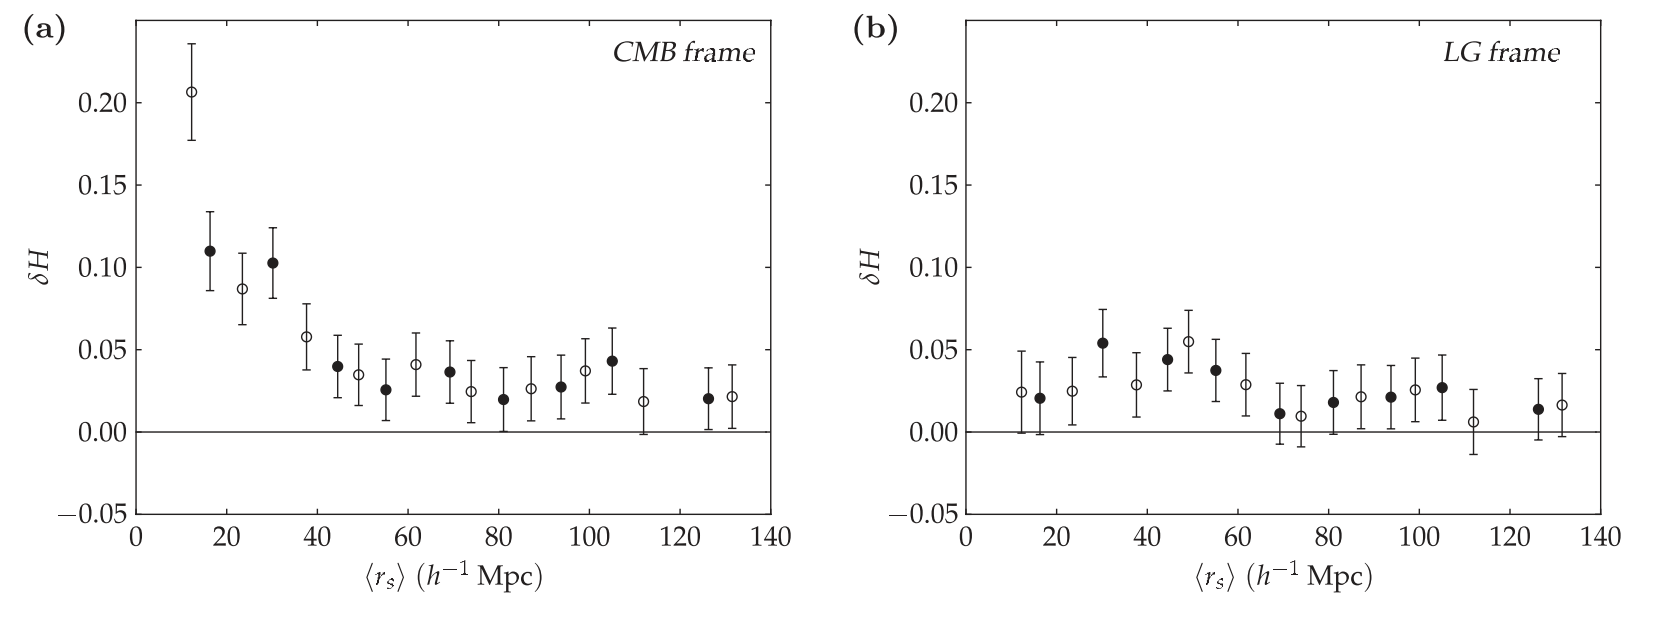
\includegraphics[width=\textwidth]{Spherically averaged Hubble constant variation Wiltshire et al 2013.png}
  \caption{Variation in the best fit Hubble constant $\delta H_s = (H_s - \bar{H}_0)/\bar{H}_0$ binned over distance for plotted against average bin distance $\langle r_s \rangle = \langle d_i \rangle$. Evaluated in: (a) the CMB frame, (b) the Local Group frame. Figure credit: Wiltshire \etal \cite{RN35}}
  \label{fig: Hubble flow variance - CMB vs LG}
\end{figure}

In \cite{RN40}, McKay and Wiltshire investigated the AIE frame and its characterisation via \eqref{\ref{eqn: diff of hubble constants}} upon arbitrary boosts of the observer, considering both the COMPOSITE and Cosmicflows-II (CF2) catalogues. They confirmed the results of Wiltshire \etal \cite{RN35} (using COMPOSITE) that the LG frame appears to be a better frame of rest than the CMB rest frame. Unfortunately, the CF2 data contains an uncorrected Malmquist bias which causes a significant difference in the calculations of $H_s$. The authors do, however, find the distinctive signature of \eqref{\ref{eqn: diff of hubble constants}} with the CF2 data, and find no reason for this to be affected by the Malmquist bias or any correction process.

Additionally, the authors find degeneracy in the frames which minimise the variation in the spherically averaged Hubble expansion. As well as the LG frame being a good fit to (\ref{eqn: diff of hubble constants}) (with some deviations, which were attributed to the presence of structures affecting the observed expansion rate), one can perform boosts of magnitude $100 - 200\, \si{km.s^{-1}}$ directed around the Zone of Avoidance without significantly changing the fit to (\ref{eqn: diff of hubble constants}). The Zone of Avoidance is the area of the sky which is taken up by the Milky Way (typically considered around $|b| \leq 10\degree$), obscuring galaxies positioned behind it, so galaxy catalogues cannot usually sample this area very well. The authors hypothesised that the degeneracy in their determined AIE frames is due to the lack of constraining data in the Zone of Avoidance.

These results were initially seen as evidence against the standard $\Lambda$CDM model. However, it was later shown that these results can also be explained by the presence of bulk flows in the standard $\Lambda$CDM model. Kraljic and Sarkar \cite{RN122} showed that in the presence of a bulk flow, \eqref{\ref{eqn: diff of hubble constants}} has an additional term,
\begin{equation} \label{eqn: diff of hubble constants with bulk flow}
  H'_s - H_s \approx \frac{v^2 - 2 \vec{v} \cdot \vec{v}_\text{bulk}(r)}{3\bar{H}_0 \langle d_i^2 \rangle_s}.
\end{equation}
This additional term originates from a dipole structure in the redshifts in the AIE frame caused by the bulk flow, interpreted as a dipole structure in the velocity field.

The subsequent reanalysis of COMPOSITE and CF2 using a standard $\Lambda$CDM model N-body simulation (specifically, Kraljic and Sarkar used the Dark Sky Simulations Early Data Release \cite{RN178}) showed that the results of \cite{RN35,RN40} are consistent with this simulation. The inclusion of a bulk flow can numerically fit the deviations from \eqref{\ref{eqn: diff of hubble constants}} in the range where structures are most nonlinear, and within underdensities of the simulation there exist candidate locations matching the observations of \cite{RN35} and \cite{RN40}. Thus the observed difference between the AIE frame and the CMB rest frame are not necessarily in conflict with $\Lambda$CDM.
This conclusion has also been reached by Bengaly \etal by analysing the CosmicFlows-3 data set with linear perturbative analysis and simulations \cite{RN123}.
Whether these simulations and conclusions match observations of bulk flows is difficult to say, as bulk flow measurements are subject to significant and increasing disagreement and controversy, as outlined in Section \ref{section: bulk flows}.

\subsection{Hubble Flow Anisotropy}\label{section: introduction - hubble flow anisotropy}
If one uses a truncation of \eqref{\ref{eqn: standard model - d_L Taylor series}} to determine the Hubble constant in a universe where differential expansion is not negligible, one will see anisotropy in the measured expansion. Several studies have shown statistically significant Hubble flow anisotropy in various data sources, including the COMPOSITE sample \cite{RN3}, galaxy clustering from eeHIFLUGCS \cite{RN121,RN106}, Type Ia supernovae data from the Pantheon compilation \cite{RN108}, the HST Extragalactic Scale Key Project \cite{RN119}, quasars, and gamma-ray bursts \cite{RN107}.

The statistic of focus for Hubble flow anisotropy in this thesis is the one used by Bolejko, Nazer, and Wiltshire \cite{RN3} (BNW). We examine the dipole and quadrupole power of fluctuations in the Hubble flow. Starting from \eqref{\ref{eqn: min chi2 H_0}}, one applies Gaussian window function smoothing over redshift and solid angle to obtain an average local Hubble constant,
\begin{equation}\label{eqn: gaussian smoothed hubble constant}
  H_0 (l, b, z) = \frac{\sum_i H_i w_{d,i} w_{z,i} w_{\theta,i}}{\sum_i w_{d,i} w_{z,i} w_{\theta,i}}.
\end{equation}
Here we use more terms in the distance-redshift Taylor expansion so that
\begin{equation}
  H_i = c \zeta_i / d_i
\end{equation}
where
\begin{equation}
  \zeta_i = z_i + \frac{1}{2}(1-q_0)z_i^2 - \frac{1}{6}(1-q_0-3q_0^2+j_0)z_i^3.
\end{equation}
The weights in \eqref{\ref{eqn: gaussian smoothed hubble constant}} are given by
\begin{align}
  w_{d,i} &= \frac{c\zeta_i}{d_i}, \\
  w_{z,i} &= \frac{1}{\sqrt{2\pi}\sigma_z}\exp\left[-\frac{1}{2}\left(\frac{z-z_i}{\sigma_z}\right)^2\right], \\
  w_{\theta,i} &= \frac{1}{\sqrt{2\pi}\sigma_\theta}\exp\left[-\frac{1}{2}\left(\frac{\theta_i}{\sigma_\theta}\right)^2\right],
\end{align}
where $\sigma_z = 0.01$ and $\sigma_\theta = 25\degree$ are the standard deviations used for the window functions, and $\theta_i$ is the angle between object $i$ and the direction of evaluation in the sky $(l,b)$ as given by
\begin{equation}
  \cos\theta_i = \cos b \cos b_i \cos(l-l_i) + \sin b \sin b_i.
\end{equation}

Over an angular and redshift grid, we analyse the fluctuation in $H_0$,
\begin{equation}
  \frac{\Delta H_0}{\langle H_0 \rangle} = \frac{H_0(l,b,z) - \langle H_0 \rangle(z)}{\langle H_0 \rangle(z)},
\end{equation}
where $\langle H_0 \rangle$ is the spherical average of $H_0(l,b,z)$ (for a particular $z$ value). In particular, we are interested in the dipole and quadrupole power ($C_1$ and $C_2$, as defined in \eqref{\ref{eqn: spherical harmonic power}}) of $\Delta H_0/\langle H_0 \rangle$. Note that the monopole contribution $C_0$ vanishes as $\Delta H_0/\langle H_0 \rangle$ has zero average by definition.

The uncertainty in the angular power spectrum is found by constructing 10,000 mock COMPOSITE catalogues, where the luminosity distance of each source within each mock catalogue is chosen randomly from a Gaussian with a standard deviation corresponding to the uncertainty in the observed luminosity distance. The analysis described above is repeated for each mock catalogue, giving a random sample of $C_1$ and $C_2$ for the chosen $z$ values. This random sample gives the uncertainty intervals seen in Figure \ref{fig: COMPOSITE dipole and quadrupole vs FLRW boosted observer}.

BNW \cite{RN3} performed this analysis for the COMPOSITE catalogue in the Local Group frame, and mock COMPOSITE catalogues generated using a boosted observer in an FLRW geometry. This was done for two boosts:

\begin{enumerate}[(i)]
  \item The expected boost from the kinematic interpretation of the CMB, with a magnitude of $635\, \si{km.s^{-1}}$.
  \item A $350\, \si{km.s^{-1}}$ boost which matches the Hubble expansion dipole of the COMPOSITE catalogue, but does not match the CMB.
\end{enumerate}

\begin{figure}[t]
  \centering
  \begin{subfigure}[b]{0.45\textwidth}
    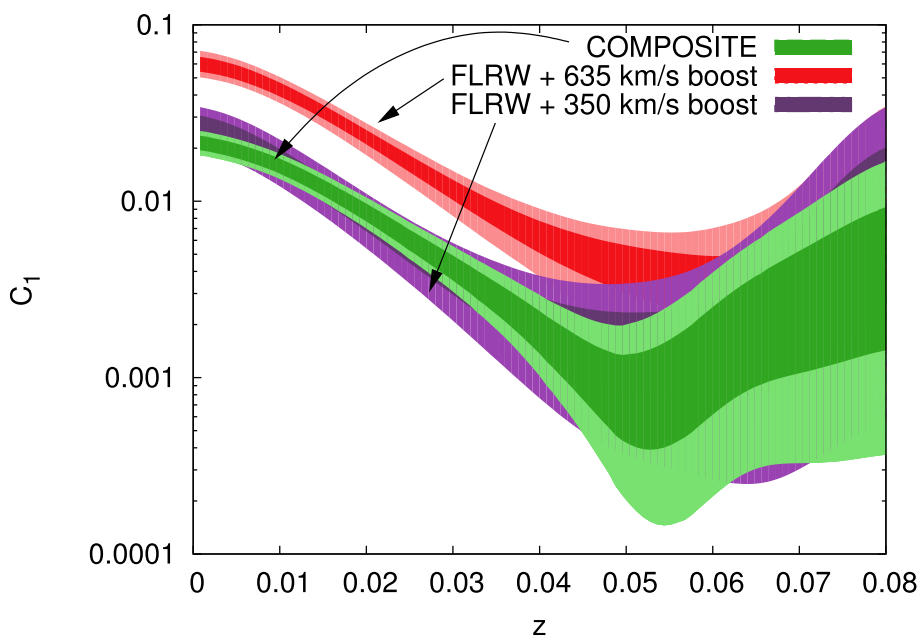
\includegraphics[width=\textwidth]{Composite Dipole Power vs FLRW with boost.png}
    \caption{}
  \end{subfigure}
  \hfill
  \begin{subfigure}[b]{0.45\textwidth}
    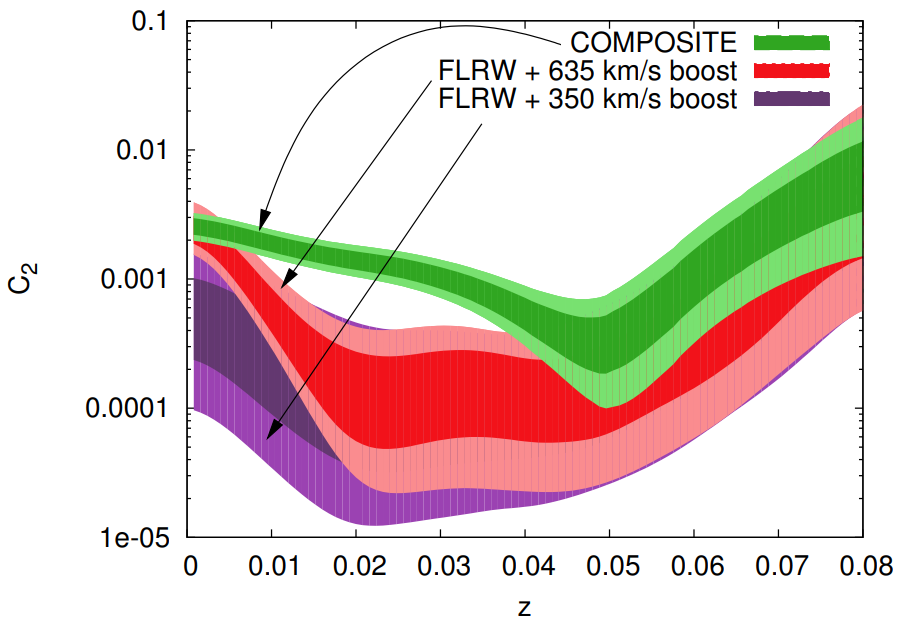
\includegraphics[width=\textwidth]{Composite quadrupole Power vs FLRW with boost.png}
    \caption{}
  \end{subfigure}
  \caption{(a) Dipole and (b) quadrupole power of $\Delta H_0/\langle H_0 \rangle$. The bands show the 65\% and 95\% confidence intervals for each $z$ value. This is calculated for the COMPOSITE catalogue in the Local Group frame, and mock COMPOSITE catalogues generated by an FLRW model with a locally boosted observer. Figure credit: Bolejko \etal \cite{RN3}}
  \label{fig: COMPOSITE dipole and quadrupole vs FLRW boosted observer}
\end{figure}

 The results can be seen in Figure \ref{fig: COMPOSITE dipole and quadrupole vs FLRW boosted observer}, and show that the dipole and quadrupole of the Hubble expansion cannot be simultaneously fit with the CMB dipole by the simple model of a boosted observer in an FLRW spacetime. The authors suggest this could be resolved by either a coherent bulk flow up to $z \sim 0.045$, or the presence of a substantial nonkinematic component in the CMB and Hubble dipole. We note that this result is not evidence against the standard model. It is reasonable to expect nearby large scale structure to cause dipole and quadrupole fluctuations in the inferred Hubble flow due to correlations of peculiar velocities, as is seen for the monopole in N-body simulations \cite{RN122}.



%%%%%%%%%%%%%%%%%%%%%%%%%%%%%%%%%%%%%%%%%%%%%%%%%%%%%%%%%%%%%%%%%%%%%%%%%%%%%%%%
%% Summary of Research
\section{Summary of Research}
In this thesis, we investigate the hypothesis that differential expansion creates a significant dipole in the CMB. We do this by simulating the effect of a void and neighbouring overdensities using exact inhomogeneous solutions of Einstein's equations, repeating and extending the work done by Bolejko, Nazer, and Wiltshire in \cite{RN3} (BNW).

In Chapter \ref{chapter: Szekeres Solutions}, we cover the background knowledge of Szekeres solutions, the family of exact inhomogeneous solutions of Einstein's equations used to model inhomogeneous structure in later chapters. Chapter \ref{chapter: BNW model analysis} presents the methods used, and a reanalysis of the model used by BNW. Chapter \ref{chapter: two structures} extends the model to include a second overdensity with the goal of making the model more realistic, and presents our analysis of this model. Finally, Chapter \ref{chapter: conclusion} concludes with a brief summary and discussion.


%%%%%%%%%%%%%%%%%%%%%%%%%%%%%%%%%%%%%%%%%%%%%%%%%%%%%%%%%%%%%%%%%%%%%%%%%%%%%%%%
\chapter{Quasispherical Szekeres Models} \label{chapter: Szekeres Solutions}
% Introduction to Szekeres Models
%%%%%%%%%%%%%%%%%%%%%%%%%%%%%%%%%%%%%%%%%%%%%%%%%%%%%%%%%%%%%%%%%%%%%%%%%%%%%%%%

The Szekeres solutions are a set of exact solutions of Einstein's equations found in 1975 \cite{RN20,RN19} which generalise the inhomogeneous spherically symmetric solutions of Lema\^itre and Tolman (LTB) \cite{RN65,RN62,RN135,RN136}. They contain only a pressureless, comoving, irrotational dust in their energy momentum tensor, i.e., $T^{\mu\nu} = \rho U^\mu U^\nu$ where $U^\mu = \delta^{\mu}_t$ in comoving coordinates, and an optional cosmological constant. Their usefulness comes from the fact that they are inhomogeneous and anisotropic exact solutions, so they can be used to model a wide range of phenomena and calculate observables in a well understood environment. The metric is given by
\begin{equation}
  ds^2 = -\diff{t}^2 + e^{2\alpha}\diff{r}^2 + e^{2\beta}(\diff{p}^2 + \diff{q}^2),
\end{equation}
where $\alpha = \alpha(t,r,p,q)$ and $\beta = \beta(t,r,p,q)$. There are two broad families of Szekeres solutions \cite{RN5}:
\begin{description}
  \item[Class 1] $\beta_{,r} \neq 0$,
  \item[Class 2] $\beta_{,r} = 0$.
\end{description}
In this thesis, we will only concern ourselves with class 1 solutions, as this is the one that has found application within cosmology \cite{RN4}. Notably, class 2 can be formulated as a limit of class 1 \cite{RN132}.

Upon solving Einstein's equations, class 1 metrics can be written as
\begin{equation}\label{eqn: szekeres - proj coords metric}
  ds^2 = -\diff{t}^2 + \frac{(R'-R\frac{\mathcal{E}'}{\mathcal{E}})^2}{\epsilon - k}\diff{r}^2 + \frac{R^2}{\mathcal{E}^2}(\diff{p}^2 + \diff{q}^2)
\end{equation}
where $R=R(t,r)$, $k=k(r)$, and $\mathcal{E}=\mathcal{E}(r,p,q)$ (see \eqref{\ref{eqn: szekeres E definition}}). In this thesis, we use the parametrisation used by Buckley and Schlegel in \cite{RN1}, which is based on the parametrisation introduced by Bolejko \etal within \cite{RN4}.

In \eqref{\ref{eqn: szekeres - proj coords metric}}, $\epsilon$ corresponds to the subtype of the model as follows:
\begin{itemize}
  \item $\epsilon = -1$: quasipseudospherical
  \item $\epsilon = 0$: quasiplanar
  \item $\epsilon = +1$: quasispherical.
\end{itemize}
The quasispherical subtype has received the most attention, and is the simplest to understand. This thesis will focus on this subtype, so from here on we set $\epsilon = +1$. For more discussion of the other subtypes, see \cite{RN5,RN134,RN133,RN4}.

The quasispherical Szekeres model can be thought of as a series of non-concentric spherical shells labelled by $r$, with $R(t,r)$ being the proper areal radius of shell $r$ at time $t$, and $k(r)$ being related to the local spatial curvature. Each shell contains the previous one, but they are shifted and rotated relative to each other \cite{RN1,RN11}.
The coordinates $p$ and $q$ are the coordinates in the plane resulting from a stereographic projection using the unit sphere centred at $p=P(r), q=Q(r)$, with a projection point $S(r)$ above the plane.
This is demonstrated in Figure \ref{fig: szekeres - stereographic projection}. Note that due to the variation of $P$, $Q$, and $S$ with $r$, the stereographic projection is different on different shells.

\begin{figure}
  \centering
  \def\svgwidth{100mm}
  \input{Figures/stereographic projection.pdf_tex}
  \caption{A diagram of the stereographic projection of the spheres onto the $(p,q)$ plane. One dimension is omitted. Red points on the sphere are projected to the blue points on the plane from the projection point at the top of the sphere.}
  \label{fig: szekeres - stereographic projection}
\end{figure}

The Szekeres solution has no Killing vectors in general \cite{RN13}; it is both inhomogeneous and anisotropic. How the isotropy is broken is determined by the `dipole functions' $S(r)$, $P(r)$, and $Q(r)$ which determine the value of $\mathcal{E}(r,p,q)$ as follows,
\begin{equation} \label{eqn: szekeres E definition}
  \mathcal{E}(r,p,q) \equiv \frac{[p-P(r)]^2+[q-Q(r)]^2+S(r)^2}{2S(r)}.
\end{equation}
We will describe how the dipole functions cause the geometry to deviate from isotropy later in this chapter.

Applying Einstein's equations to the metric gives a Friedmann-like evolution equation for $R(t,r)$\footnote{This is identical to that of the spherically symmetric LTB limit.}
\begin{equation}\label{eqn: szekeres - evolution equation}
  \dot{R}(t,r)^2 = \frac{2M(r)}{R(t,r)} - k(r) + \frac{1}{3}\Lambda R(t,r)^2,
\end{equation}
and a mass density
\begin{equation} \label{eqn: szekeres - mass density equation}
  4\pi G \rho(t,r,p,q) = \frac{M'(r)-3M(r)\frac{\mathcal{E}'(r,p,q)}{\mathcal{E}(r,p,q)}}{R(t,r)^2\left[R'(t,r)-R(t,r)\frac{\mathcal{E}'(r,p,q)}{\mathcal{E}(t,p,q)}\right]}.
\end{equation}
Note the lack of homogeneity and isotropy on account of the dependence of $\mathcal{E}'/\mathcal{E}$ on all spatial coordinates. In this chapter, $'=\pderiv{}{r}$ where $p, q,$ and $t$ are held constant, and $\dot{}=\pderiv{}{t}$ as before. The function $M(r)$ appears as a function of integration when integrating Einstein's equations, and acts like the total effective gravitational mass\footnote{The function $M(r)$ is not the three-dimensional integral of the mass density $\rho$ that one would expect, as seen from the lack of $k(r)$ in the density equation. However, it is $M(r)$ that appears in the evolution \eqref{\ref{eqn: szekeres - evolution equation}}, therefore we refer to it as the effective gravitational mass rather than simply the total mass.} inside the shell of radius $r$. From the likeness of \eqref{\ref{eqn: szekeres - evolution equation}} to the Friedmann equation (\ref{eqn: Friedmann Equation 1}), we infer that each shell evolves like a constant-$r$ surface of a pressureless FLRW geometry. However, as the parameters vary with $r$, their evolution is somewhat independent. We integrate (\ref{eqn: szekeres - evolution equation}) to get
\begin{equation}\label{eqn: bang time integral}
  t-t_B(r) = \int_0^{R(t,r)}\frac{\diff{\tilde{R}}}{\sqrt{2M(r)/\tilde{R} - k(r) + \Lambda \tilde{R}^2/3}},
\end{equation}
where $t_B(r)$ is another function of integration, called the `bang-time function' as it is defined such that $R(t_B(r),r)=0$. Unlike FLRW geometries, but like LTB geometries, Szekeres geometries can have a `nonsimultaneous big bang', where shells encounter the singularity $R=0$ at different times.

To define a Szekeres model, we need to set $M$, $k$, $t_B$, $P$, $Q$, and $S$, giving the model an apparent 6 functional degrees of freedom. However, $r$ is just a label in the sense that the form of the metric and evolution equations are invariant under a transformation $r \to \tilde{r}=f(r)$ for a monotonic $f$. This is a gauge freedom with which we can impose a definition of $r$ without affecting the physical geometry. This creates a physical equivalence between Szekeres models, reducing the number of functional degrees of freedom to 5. There is no canonical choice, and any choice somewhat restricts the range of available models. One convenient choice is $M(r)=r^3$, which cannot accommodate a vacuum over a range of $r$. The choice $R(t_0,r)=r$ is also convenient, but forces $R$ to be monotonic in $r$, ruling out closed universes and wormhole topologies. In this thesis we are interested in the geometry of the local neighbourhood, which does not contain such features, so we will use this latter choice.


\section{Spherical Polar Coordinates}
The Szekeres geometry can be written in more familiar spherical polar coordinates $(\theta, \phi)$ instead of the projective coordinates $(p,q)$. With the projection point where $p$ and $q$ diverge at $\theta=0$, the coordinate transform is
\begin{align}\label{eqn: Szekeres - spherical coordinate transformation}
  p-P(r)&=S(r)\cot\left(\frac{\theta}{2}\right)\cos\phi, & q-Q(r)&=S(r)\cot\left(\frac{\theta}{2}\right)\sin\phi.
\end{align}
One could instead use a transformation where the projection point is at $\theta=\pi$ by swapping $\cot$ for $\tan$, but for this thesis we will use (\ref{eqn: Szekeres - spherical coordinate transformation}). In these coordinates, the metric takes the more complicated form
\begin{align} \label{eqn: szekeres spherical coords metric}
  ds^2 = &-\diff{t}^2 \\
  &+ \left[\frac{\left(R' - R\frac{\mathcal{E}'}{\mathcal{E}}\right)^2}{1-k} + R^2(1-\cos\theta)^2
  \left(\frac{P'^2 + Q'^2 + S'^2}{S^2} - \frac{2}{1-\cos\theta}\frac{S'}{S}\frac{\mathcal{E}'}{\mathcal{E}}\right)\right]\diff{r}^2 \nonumber\\
  &+ \frac{R^2\sin\theta}{1+\cos\theta}\left(\frac{\mathcal{E}'}{\mathcal{E}} - \frac{S'}{S}\right)\left(\diff{r}\diff{\theta} + \diff{\theta}\diff{r}\right) \nonumber\\
  &+ \frac{R^2 \sin^3\theta}{1+\cos\theta}\left(\frac{Q'}{S}\cos\phi - \frac{P'}{S}\sin\phi\right)\left(\diff{r}\diff{\phi} + \diff{\phi}\diff{r}\right)
  + R^2 \left(\diff{\theta}^2 + \sin^2\theta\diff{\phi}^2\right),
\end{align}
here $'$ still refers to a partial derivative with respect to $r$ whilst holding $p$ and $q$ constant, not $\theta$ and $\phi$. This form provides some clarity on the physical geometry of the model. Note that on a shell (taking $\diff{r}=\diff{t}=0$), the metric is,
\begin{equation}
  dl^2 = R^2 \left(\text{d}\theta^2 + \sin^2\theta\diff{\phi}^2\right)
\end{equation}
so the shells are indeed spheres. When restricted to a shell, it can be useful to define a \textit{local rectangular frame} (LRF) by
\begin{align}\label{eqn: szekeres - LRF definition}
  x &\equiv \sin\theta\cos\phi, & y&\equiv \sin\theta\sin\phi, & z&\equiv\cos\theta.
\end{align}

In spherical coordinates, $\mathcal{E}$ takes the following simpler form
\begin{equation}
  \mathcal{E}(r,\theta,\phi) = \frac{S(r)}{1-\cos\theta},
\end{equation}
and $\mathcal{E}'/\mathcal{E}$, as found in the density equation (\ref{eqn: szekeres - mass density equation}), takes the form
\begin{equation}
  \frac{\mathcal{E}'}{\mathcal{E}} = -\frac{S'\cos\theta + P'\sin\theta\cos\phi + Q'\sin\theta\sin\phi}{S},
\end{equation}
showing that $S'/S$, $P'/S$, and $Q'/S$ define an isotropy on the shell in the $z, x,$ and $y$ directions respectively.

\section{The FLRW and LTB Limits} \label{section: szekeres - geometry limits}
The family of Szekeres solutions contains other notable exact solutions of Einstein's equations. In particular, it contains the Lemaître-Tolman-Bondi (LTB) and pressureless FLRW solutions.

If one chooses $S'=P'=Q'=0$ so that $\mathcal{E}'/\mathcal{E} = 0$, then the metric in spherical coordinates (\ref{eqn: szekeres spherical coords metric}) reduces to
\begin{equation}
  ds^2 = -\diff{t}^2 + \frac{(R')^2}{1 - k}\diff{r}^2 + R^2 \left(\diff{\theta}^2 + \sin^2\theta\diff{\phi}^2\right).
\end{equation}
This is the metric of the LTB models \cite{RN62,RN135,RN136}. It has spherical symmetry, but has radial inhomogeneity. It has seen much application in modelling the effects of voids \cite{RN5,RN4}. In particular, research into LTB void models without a cosmological constant or other dark energy model showed that the accelerating expansion of the Universe cannot solely be explained by our presence within a large void \cite{RN128,RN129,RN130,RN131,RN127}\footnote{C\'el\'erier, Bolejko, and Krasi\'nski (2010) \cite{RN146} showed that a $\Lambda=0$ LTB geometry with a central overdensity rather than a central void can replicate the Hubble flow expected in $\Lambda$CDM without the need for dark energy. However, this requires a strongly non-simultaneous big-bang $t_B \neq 0$, possibly creating large-scale inhomogeneities in the past which conflict with CMB measurements and the inflationary paradigm \cite{RN195,RN196,RN140}.}. There was also an attempt to resolve the Hubble tension using LTB models possessing a cosmological constant (see \cite{RN137} Section VII-H-3 and references therein). However, thus far this approach appears to be unsuccessful.

To recover the isotropic and homogenous FLRW geometry (\ref{eqn: FLRW metric}), one additionally sets $t_B(r) = \text{constant}$, and $|k(r)|^{3/2}/M(r) = \text{constant}$ \cite{RN4}. There is then a choice of the coordinate $r$ such that
\begin{align}
  M(r) &= M_0 r^3, \\
  \Longrightarrow k(r) &= k_0 r^2,
\end{align}
where $M_0$ and $k_0$ are constants related to the FLRW parameters by
\begin{align}
  M_0 &= \frac{1}{2}H_0^2 \Omega_{M0} \\
  k_0 &= H_0^2(\Omega_{M0} + \Omega_{\Lambda 0} - 1).
\end{align}
\eqref{\ref{eqn: szekeres - evolution equation}} then has a solution of the form $R(t,r) = r\,a(t)$, from which the Friedmann equation can be recovered.

It is possible to choose a Szekeres model such that beyond a certain critical $r$ value, the geometry is identical to an LTB or FLRW metric, creating a `patch' of inhomogeneity and anisotropy within an otherwise symmetrical background geometry. One common use for this is in Swiss-cheese models, where many LTB or Szekeres model patches are placed in an FLRW background to create a model of large scale structure (e.g. see \cite{RN142,RN141,RN140}).


\section{Departure from Isotropy} \label{section: szekeres - anisotropy}
In some sense, the quasispherical Szekeres solution is a generalisation of the LTB models, where the departure from isotropy is determined by $\mathcal{E}'/\mathcal{E}$. We can see this in the density equation (\ref{eqn: szekeres - mass density equation}), where the only dependence on $p$ and $q$ (or $\theta$ and $\phi$) is through $\mathcal{E}'/\mathcal{E}$. Note how we got an isotropic (LTB) geometry in Section \ref{section: szekeres - geometry limits} when we set $\mathcal{E}'/\mathcal{E} = 0$.

In projective coordinates, $\mathcal{E}'/\mathcal{E}$ takes the form
\begin{equation}\label{eqn: szekeres - E'/E projective}
  \frac{\mathcal{E}'}{\mathcal{E}} = -2\frac{P'(p-P) + Q'(q-Q) - S'S}{(p-P)^2 + (q-Q)^2 + S^2} - \frac{S'}{S}.
\end{equation}
However, it is much easier to interpret in spherical coordinates,
\begin{equation}\label{eqn: szekeres - E'/E spherical}
  \frac{\mathcal{E}'}{\mathcal{E}} = -\frac{S'}{S}\cos\theta - \frac{P'}{S}\sin\theta\cos\phi - \frac{Q'}{S}\sin\theta\sin\phi.
\end{equation}
Here we clearly see that $\mathcal{E}'/\mathcal{E}$ is a dipole on each shell where $r$ is fixed, with the functions ${S'/S}$, ${P'/S}$, and ${Q'/S}$ directly determining that dipole's amplitude and direction. The amplitude of this dipole is
\begin{equation}\label{eqn: szekeres - E'/E amplitude}
  \left(\frac{\mathcal{E}'}{\mathcal{E}}\right)_{\text{max}} = \frac{\sqrt{(P')^2 + (Q')^2 + (S')^2}}{S},
\end{equation}
and the maximum points in the direction\footnote{Here $\text{sgn}$ gives the sign of its argument. So $\text{sgn}(x)$ is $1$ if $x$ is positive, $-1$ if $x$ is negative, and $0$ if $x=0$.}
\begin{subequations}
  \begin{align}\label{eqn: szekeres - E'/E direction spherical}
    \theta_{\text{max}} = \cos^{-1}\left(-\frac{S'}{\sqrt{(P')^2 + (Q')^2 + (S')^2}}\right), \\
    \phi_\text{max} = -\text{sgn}(Q')\cos^{-1}\left(-\frac{P'}{\sqrt{(P')^2 + (Q')^2}}\right).
  \end{align}
\end{subequations}
In projective coordinates,
\begin{equation}\label{eqn: szekeres - E'/E direction projective}
  (p,q)_\text{max} = (P,Q) - \frac{(P',Q')}{S'/S + (\mathcal{E}'/\mathcal{E})_\text{max}}.
\end{equation}

These dipole functions have three main effects on the geometry, they shift the relative position of the shells, rotate them, and affect the distribution of matter \cite{RN12,RN11,RN1,RN2}.

\subsection{Shell Shifting and Shell Rotation}
The dipole functions shift the constant-$r$ shells so that they are non-concentric and closer to each other on one side than on the other. The simplest way to see this is in the projective coordinates metric. Because the metric is diagonal, the (constant time) path of shortest proper distance between two shells $r_1$ and $r_2$ has constant $p$ and $q$. The shortest proper distance when $r_2 - r_1 = \delta r$ is small can be seen directly from the metric as

\begin{align}
  \delta \ell  &= \sqrt{g_{rr}}\delta r, \\
            &= \frac{R' - R\mathcal{E}'/\mathcal{E}}{\sqrt{1-k}} \delta r, \\
            &= \frac{R'}{\sqrt{1-k}} \delta r - \frac{R}{\sqrt{1-k}}\frac{\mathcal{E}'}{\mathcal{E}} \delta r. \label{eqn: szekeres - shell displacement 1}
\end{align}

When $\mathcal{E}'/\mathcal{E} = 0$, $\delta \ell$ is constant over each shell with a value of $R' \delta r/\sqrt{1-k}$. But for a non-vanishing $\mathcal{E}'/\mathcal{E}$, $\delta\ell$ varies over the shell. Thus, the shells are non-concentric. Note how the separation between two shells has its maximum and minimum corresponding with the extrema of the Szekeres dipole $\mathcal{E}'/\mathcal{E}$. By substituting in \eqref{\ref{eqn: szekeres - E'/E spherical}} for $\mathcal{E}'/\mathcal{E}$, we see that $S'/S, P'/S,$ and $Q'/S$ cause a displacement in the directions
$\theta = \{0, \pi\}$;
$\theta = \pi/2$, $\phi = \{0,\pi\}$; and
$\theta = \pi/2$, $\phi=\{\pi/2, 3\pi/2\}$ respectively. These are the $z, x,$ and $y$ directions in the LRF. The corresponding proper distances that nearby shells are shifted relative to each other are,
\begin{subequations}
  \begin{align}
    \delta_x = \frac{R}{\sqrt{1-k}} \frac{S'}{S} \delta r, \\
    \delta_y = \frac{R}{\sqrt{1-k}} \frac{P'}{S} \delta r, \\
    \delta_z = \frac{R}{\sqrt{1-k}} \frac{Q'}{S} \delta r.
  \end{align}
\end{subequations}

When $P'$ or $Q'$ is non-zero, the angular coordinates of the shells are also rotated with respect to each other. This was first noticed by Hellaby \cite{RN11} when examining orthonormal frames. This shell rotation affects the direction of shell shifting, so is important to account for when creating a representative plot (see Section \ref{section: szekeres - plotting}). The effects of shell shifting and rotation can be seen when plotting geodesics along a cross-section of the geometry. The geodesics appear very curved when plotted na\"ively or with solely shell shifting accounted for, but almost straight when both shell rotation and shell shifting are included \cite{RN1}.
Figure \ref{fig: szekeres - shell shifting and rotation} shows an illustration of shell shifting and rotation for an example geometry.

\begin{figure}[t]
  \centering
  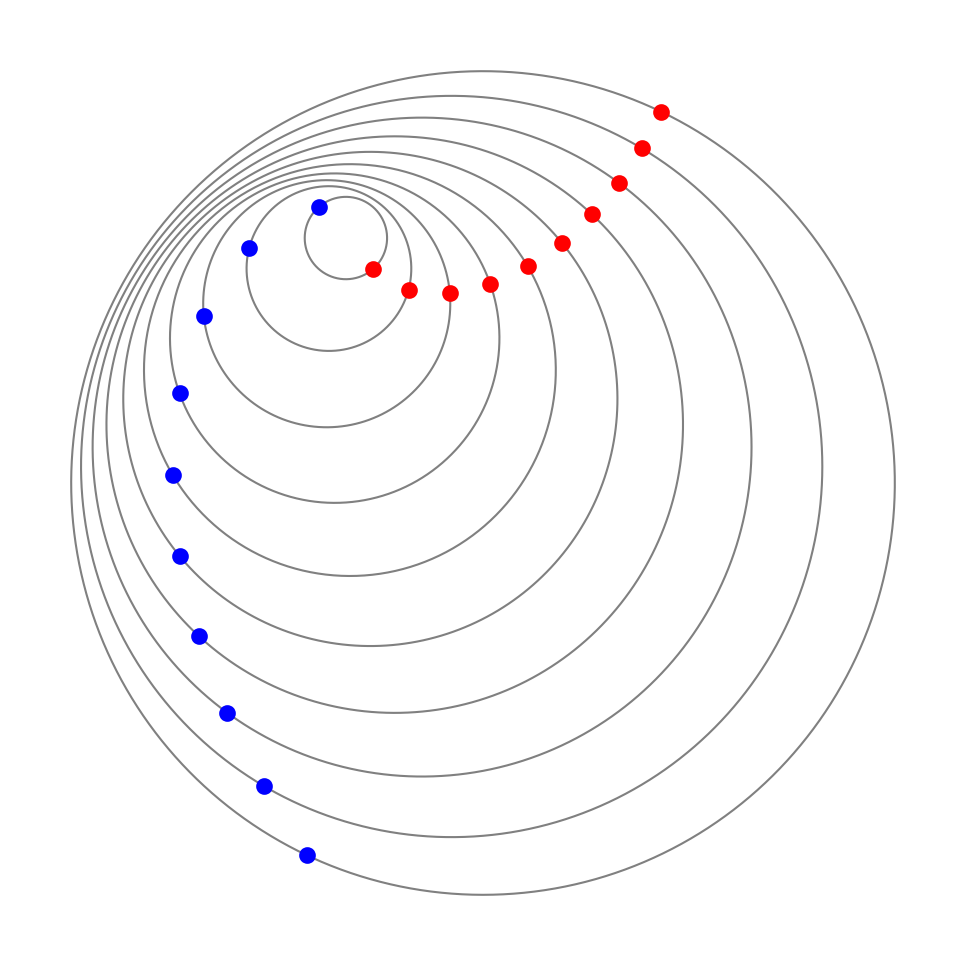
\includegraphics[width=0.45\textwidth]{shell rotation and shifting example.png}
  \caption{An illustration of several shells, showing the effects of shell shifting and shell rotation for a model with $Q=0$, $S=1$, and $P'/S = 0.8/r$. The red dots indicate the positions of $\theta=0$ on each shell, and the blue dots indicate the positions of $\theta = \pi$ on each shell.}
  \label{fig: szekeres - shell shifting and rotation}
\end{figure}

In \cite{RN1,RN2} these effects are quantified and put in context of an embedding of the constant-$t$ hypersurfaces into a 4-dimensional Euclidean space. In this context, the terms rotation and shifting can be interpreted more intuitively, having a natural global meaning where outer shells are rotated and shifted with respect to the innermost shells. When constructing the embedding an additional effect of the dipole functions is revealed, they tilt the constant-$r$ shells in the fourth spatial dimension of the embedding in a manner dependent on the dipole functions and $k$.

\subsection{The Matter Dipole}
The dipole functions clearly affect the matter density, as seen by the presence of $\mathcal{E}'/\mathcal{E}$ in the density equation (\ref{eqn: szekeres - mass density equation}). One can split the density equation into a monopole and dipole moment on each shell, i.e.,
\begin{equation}
  \rho(t,r,p,q) = \rho_{\text{mono}}(t,r) + \Delta\rho(t,r,p,q).
\end{equation}
We can reach this form by introducing an arbitrary function $H(t,r)$, then proceeding as follows
\begin{subequations}
  \begin{align}
    4\pi G \rho(t,r,p,q) &= \frac{M'-3M\frac{\mathcal{E}'}{\mathcal{E}}}{R^2\left(R'-R\frac{\mathcal{E}'}{\mathcal{E}}\right)} + \frac{H}{R^2} - \frac{H}{R^2}, \\
    &= \frac{H}{R^2} + \frac{(M'-HR')+(HR-3M)\frac{\mathcal{E}'}{\mathcal{E}}}{R^2\left(R'-R\frac{\mathcal{E}'}{\mathcal{E}}\right)}.
  \end{align}
\end{subequations}
The first term corresponds to $\rho_{\text{mono}}$ and the second to $\Delta\rho$. This splitting is obviously not unique as is, since it depends on the choice of $H$. Bolejko \etal \cite{RN4} determines $H$ by requiring that $\Delta\rho=0$ along some great circle for each shell. It turns out that with this choice of $H$, $\Delta\rho$ changes sign when crossing this great circle, so $\Delta \rho$ is a dipole-like contribution to the density equation.
These features can be seen in Figure \ref{fig: szekeres - density on shell varying dipole}, where $\rho=\rho_\text{mono}$ for $S'/S=0$, and the dipole-like contribution appears for larger values of $S'/S$.

\begin{figure}[t]
  \centering
  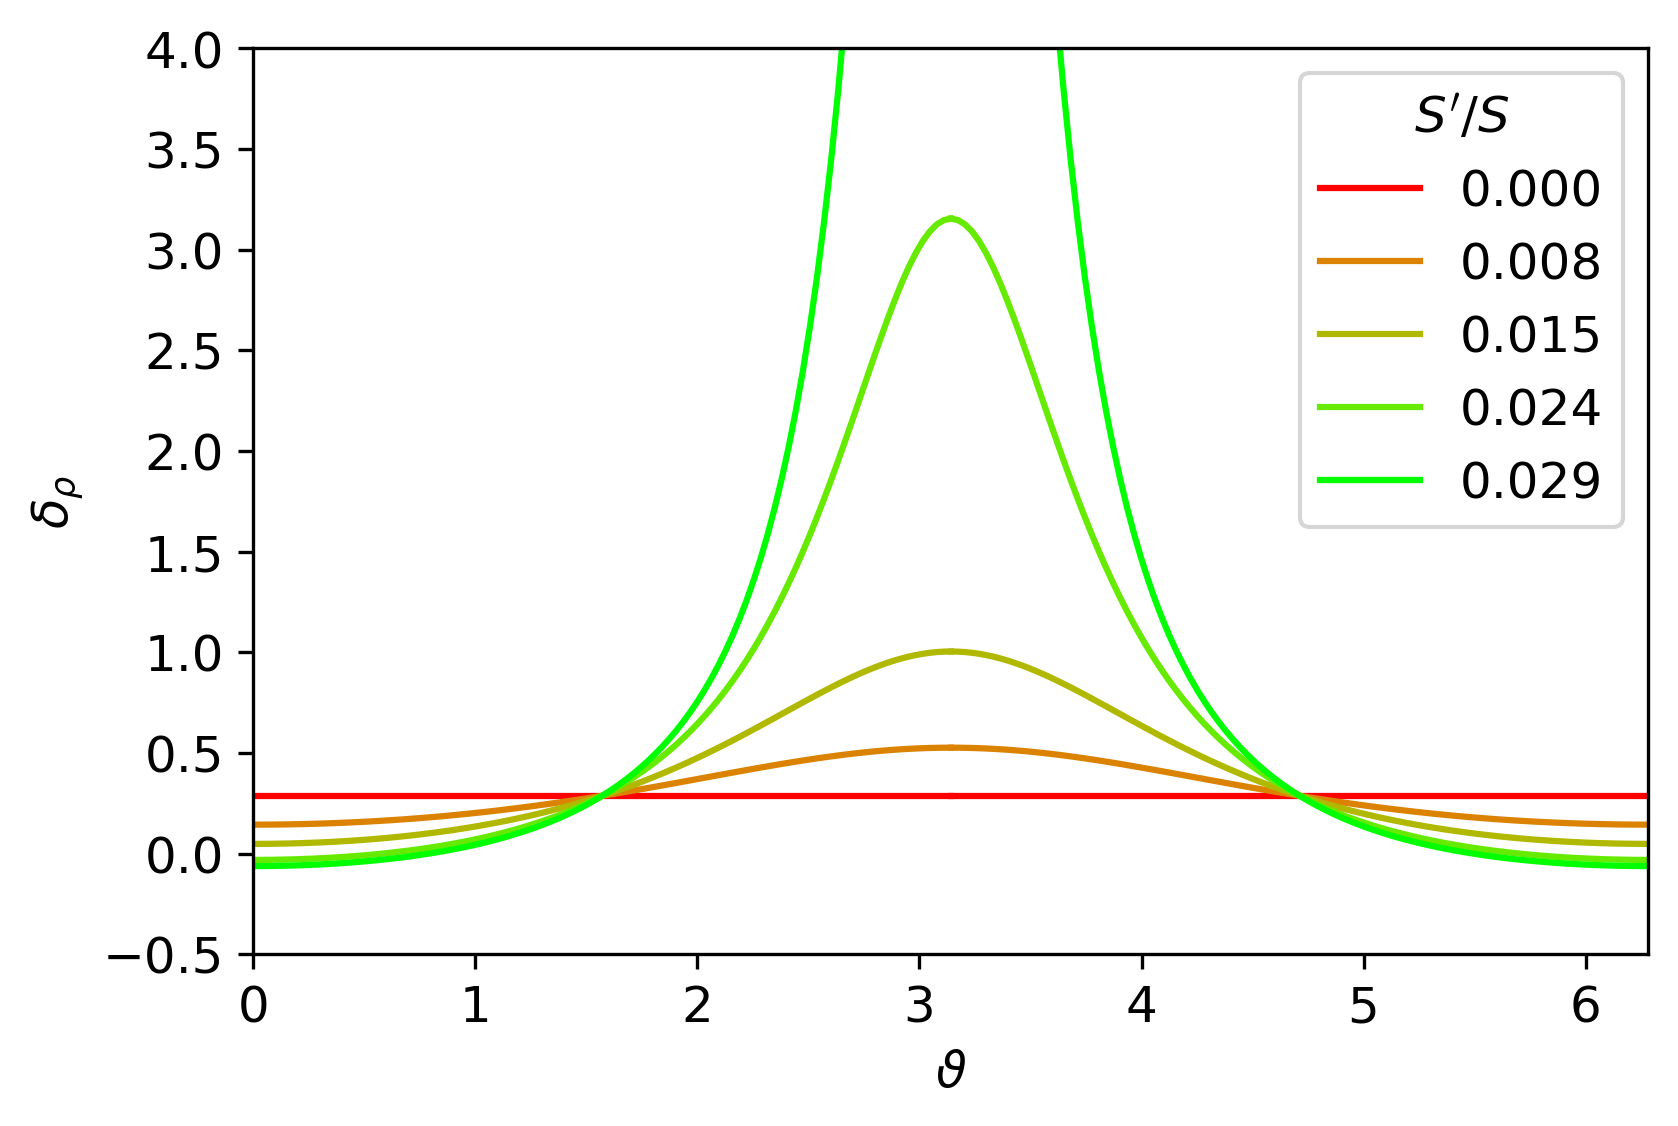
\includegraphics[width=105mm]{Density on shell varying dipole.png}
  \caption{Mass density contrasts $\delta_\rho = (\rho - \rho_\text{bg})/\rho_\text{bg}$ along a shell cross-section, where $\rho_\text{bg}$ is a background reference density. The $x$-axis variable is an angular parameterisation of the path around the shell, where $(\theta,\phi)=(\vartheta,0)$ for $\vartheta<\pi$, and $(\theta,\phi)=(2\pi-\vartheta,\pi)$ for $\vartheta \geq \pi$. The density contrast is plotted for a variety of values of $S'/S$.
  This is taken at $r=r_0=33.0$, so as $S'/S$ approaches $1/r_0 \approx 0.030$ we get a large spike at the maximum of $\mathcal{E}'/\mathcal{E}$ ($\theta=\pi$).
  At $\theta=\pi/2$, $\Delta\rho=0$ vanishes, so the only contribution is from $\rho_{\text{mono}}$, elsewhere $\Delta\rho$ has a visible contribution.
  This plot uses the axisymmetric BNW model seen in Chapter \ref{chapter: BNW model analysis} where $P=Q=0\neq S$.}
  \label{fig: szekeres - density on shell varying dipole}
\end{figure}

This dipole component can be interpreted as the result of two effects: the effect of shell shifting on density, which is reflected in the denominator of the density equation; and a dipolar redistribution of matter on each shell so that the shells maintain their spherical shape and FLRW-like evolution, reflected in the numerator of the density equation. See \cite{RN1} for details on this.


\section{Physical Restrictions}\label{section: szekeres - physical restrictions}
As stated before, a Szekeres model is specified by its 5 functional degrees of freedom. However, there are a number of physical restrictions placed on these functions to avoid non-physical behaviour such as singularities. These are listed here as stated in \cite{RN1,RN4} and put in context of the models investigated in later chapters, where we choose $R(t_0,r)=r$ (fixing the gauge freedom), and have $k(r)<0$.

\subsubsection{Differentiability}
All the free functions, in our case $S(r), P(r), Q(r), M(r)$ and $t_B(r)$ must be differentiable. $R(t_0,r)=r$ is clearly differentiable, and $k(r)$ inherits its differentiability from the other functions via \eqref{\ref{eqn: bang time integral}}.

\subsubsection{Lorentzian Signature}
We can see from the metric (\ref{eqn: szekeres - proj coords metric}) that for the Lorentzian signature $(-,+,+,+)$ to be maintained throughout the geometry we must have $k(r)\leq 1$, with equality only when $R'-R\mathcal{E}'/\mathcal{E} = 0$. There are further conditions to ensure the Lorentzian signature is maintained when you have a shell $r^*$ where $k(r^*)=1$ \cite{RN143}. However, for the models used in this thesis we have $k\leq 0$, so the Lorentzian signature is preserved.

\subsubsection{Positive Radius}
For all $(t,r)$ we must have $R(t,r) \geq 0$. During bang and crunch times and at origins, we have $R=0$, and all other shells must have positive size.

\subsubsection{Projective Mapping Restriction}
We must have $S(r) \neq 0$, or the projection mapping will fail. This condition can be violated at origins, but nowhere else. If $S = 0$ on some shell, then $\mathcal{E}$ diverges on that shell, which creates problems for the metric in both forms given thus far. Since $S$ is continuous, this condition implies $S$ cannot change sign. For models investigated in this thesis, we choose $S > 0$.

\subsubsection{Regular Origin Conditions}
An origin in a Szekeres model is a point where $R$ vanishes (excluding the bang or crunch times). It is possible for a Szekeres model to have 0, 1, or 2 origins. In this thesis, the models only have one origin, at $r=0$. Hellaby and Krasi\'nski \cite{RN143} showed that near the origins (i.e., as $r \to 0$) one must have
\begin{align} \label{eqn: szekeres - regular origin conditions}
  M &\sim R^3, & k &\sim R^2, & (S,P,Q) &\sim R^\alpha,
\end{align}
where $0 \leq \alpha \leq 1$. These conditions ensure finite density and curvature at the origin, and smooth matching to the evolution around the origin.

\subsubsection{Non-negative Mass Density}
Typically, negative mass is seen as non-physical, so is undesirable in models of realistic structure. By inspection of the density equation (\ref{eqn: szekeres - mass density equation}) we see that to have $\rho > 0$, $M'-3M\mathcal{E}'/\mathcal{E}$ and $R'-R\mathcal{E}'/\mathcal{E}$ must have the same sign. In the models considered in this thesis, $R'-R\mathcal{E}'/\mathcal{E} > 0$, so we must have
\begin{equation} \label{eqn: szekeres - non-negative mass condition 1}
  M'-3M\mathcal{E}'/\mathcal{E} \geq 0.
\end{equation}
Considering the range of values $\mathcal{E}'/\mathcal{E}$ takes on each shell, as explored in Section \ref{section: szekeres - anisotropy}, the condition (\ref{eqn: szekeres - non-negative mass condition 1}) is equivalent to satisfying
\begin{equation}
  \frac{\sqrt{(P')^2 + (Q')^2 + (S')^2}}{S} \leq \left|\frac{M'}{3M}\right|
\end{equation}
for all $r$.

\subsubsection{No Shell Crossings}
The evolution of the geometry can cause shell crossings, where one shell passes through another and creates a coordinate degeneracy where geodesics cross. At such a point, the dust particles would have different velocities at the same position, which violates the foundational assumptions of the model \cite{RN144,RN1}. Shell crossings occur if $R'-R\mathcal{E}'/\mathcal{E} = 0$ at any point besides regular extrema -- these are points which satisfy the regular origin conditions (\ref{eqn: szekeres - regular origin conditions}), so have a finite density.

Using the range of values $\mathcal{E}'/\mathcal{E}$ takes on a shell, to have a model with no shell crossings we must satisfy
\begin{equation}\label{eqn: no shell crossings condition}
  \frac{\sqrt{(P')^2 + (Q')^2 + (S')^2}}{S} \leq \frac{R'}{R}
\end{equation}
for all $(t,r)$. Hellaby and Krasi\'nski \cite{RN143} give conditions on $M, t_B,$ and $k$ which ensure the above is satisfied globally for Szekeres models with $\Lambda=0$.

\section{The Dust Congruence in Szekeres Models}
The inhomogeneity of Szekeres models causes their expansion rates to be spatially inhomogeneous and anisotropic. We quantify the expansion by examining the dust's timelike geodesic congruence. The deviation of nearby geodesics from each other is described by ${U^\mu}_{;\nu}$. To examine how ${U^\mu}_{;\nu}$ distorts the shape of the congruence, it decomposed into its trace, trace-free symmetric, and antisymmetric components,
\begin{equation}
  U_{\mu;\nu} = \frac{1}{3}\theta P_{\mu\nu} + \sigma_{\mu\nu} + \omega_{\mu\nu},
\end{equation}
where $P_{\mu\nu} = g_{\mu\nu}  + U_\mu U_\nu$ projects tensors onto spatial sections orthogonal to $U^\mu$. The trace $\theta$ is known as the expansion, which describes the change in volume over time. For dust in Szekeres models, it takes the form
\begin{equation}
  \theta \equiv {U^{\alpha}}_{;\alpha} = 2H_\perp + H_\parallel,
\end{equation}
where
\begin{equation}
  H_\perp = \frac{\dot{R}}{R}
\end{equation}
is the transverse expansion along a shell's surface, and
\begin{equation}
  H_\parallel = \frac{\dot{R}' - \dot{R}\mathcal{E}'/\mathcal{E}}{R'-R\mathcal{E}'/\mathcal{E}}
\end{equation}
is the longitudinal expansion between shells. See Figure \ref{fig: szekeres - expansion plot} for an example of how these vary in an example Szekeres model.
\begin{figure}[t]
     \centering
     \begin{subfigure}[b]{0.45\textwidth}
         \centering
         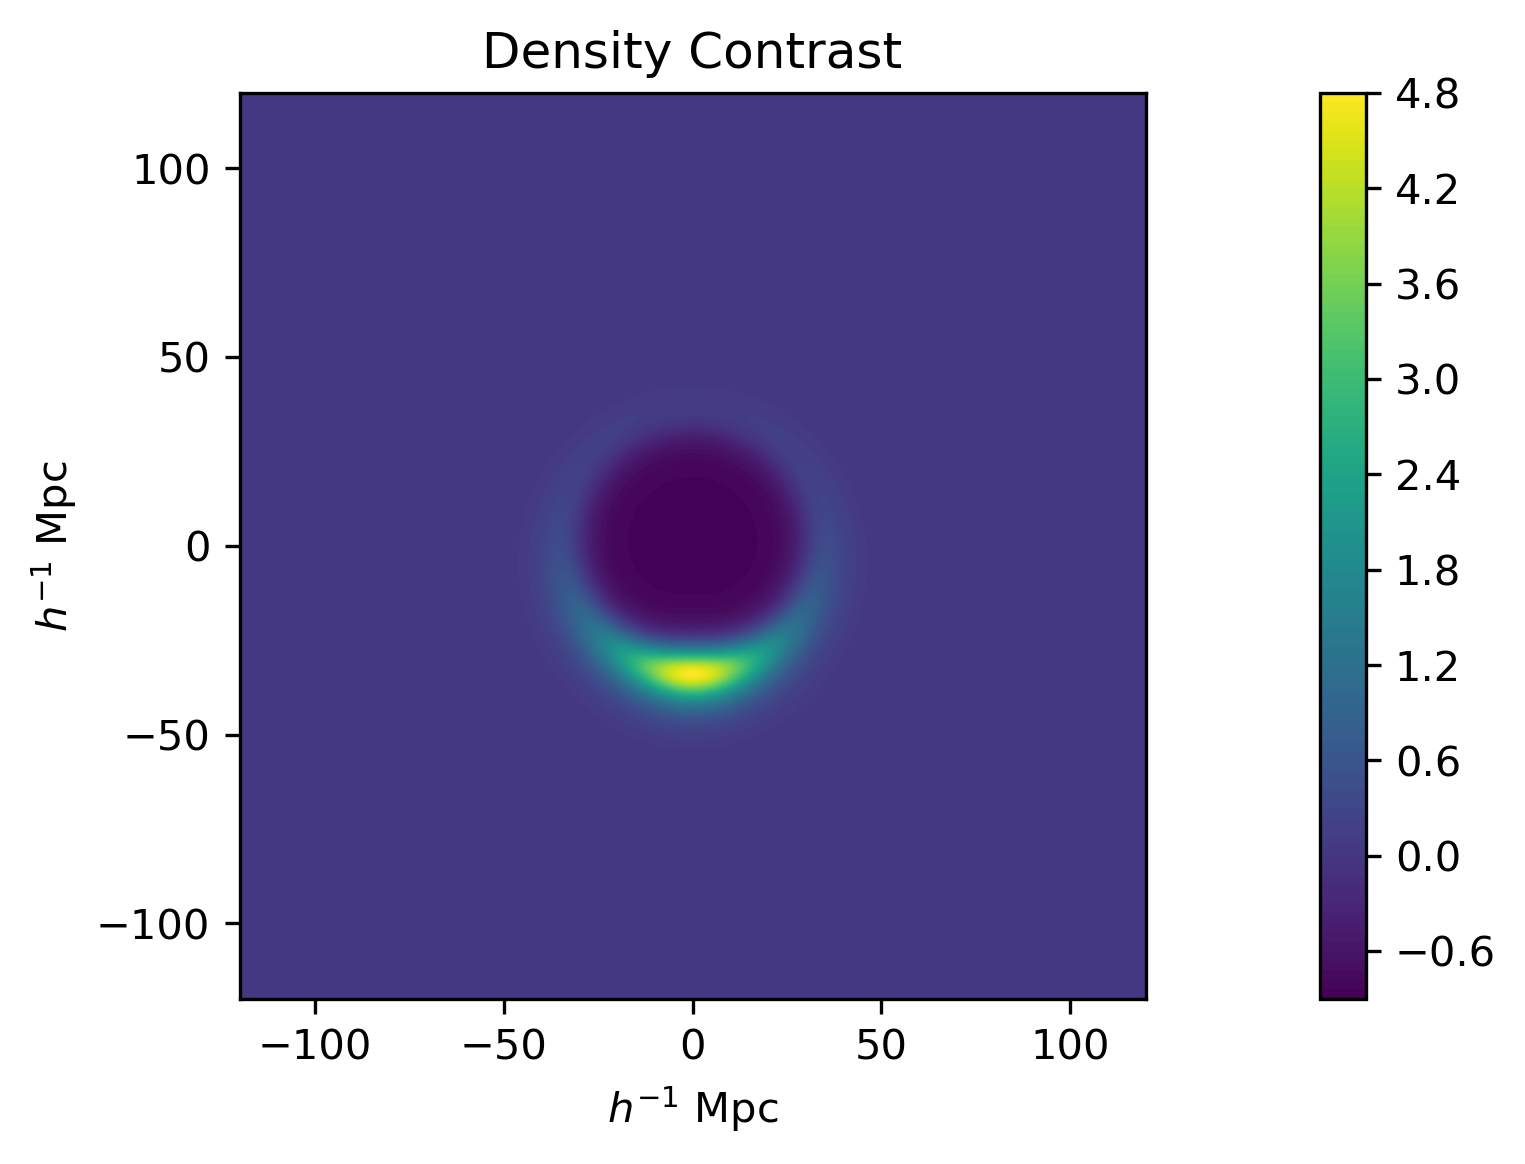
\includegraphics[width=\textwidth]{Density Contrast.png}
         \subcaption{}
     \end{subfigure}
     \hfill
     \begin{subfigure}[b]{0.45\textwidth}
         \centering
         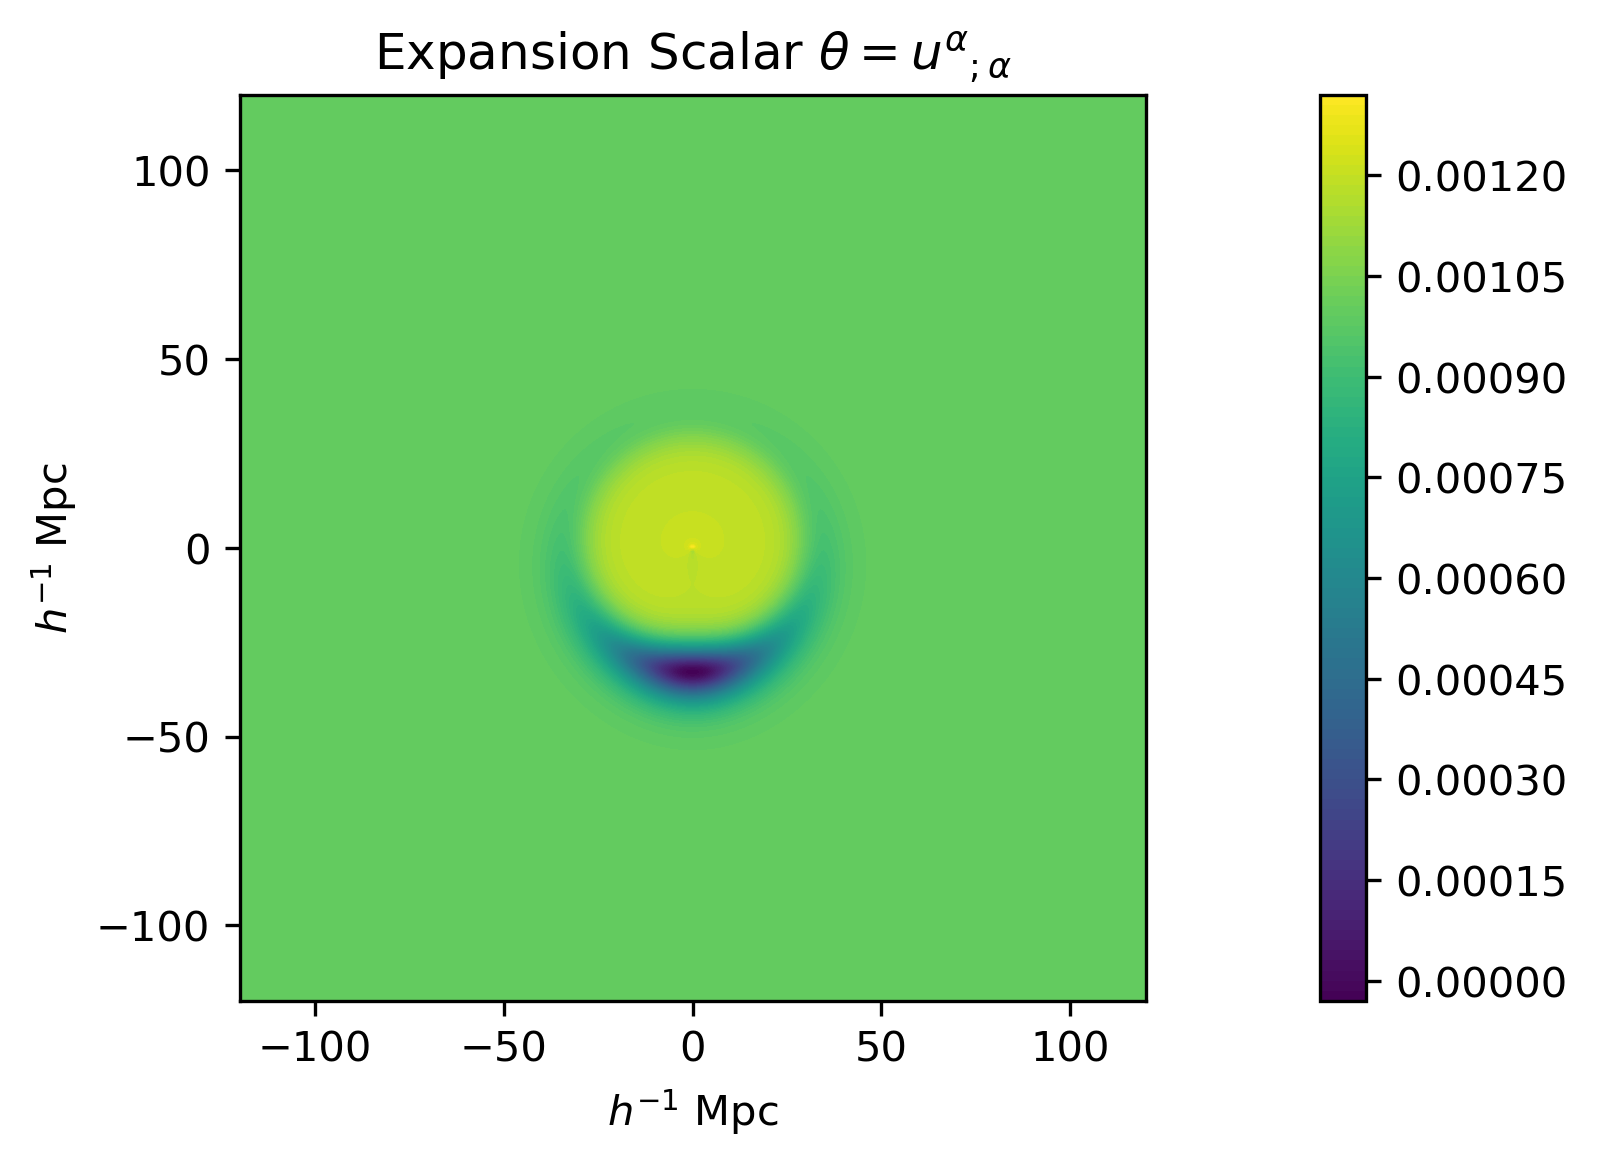
\includegraphics[width=\textwidth]{Expansion Scalar.png}
         \subcaption{}
     \end{subfigure}
     \\
      \centering
      \begin{subfigure}[b]{0.45\textwidth}
          \centering
          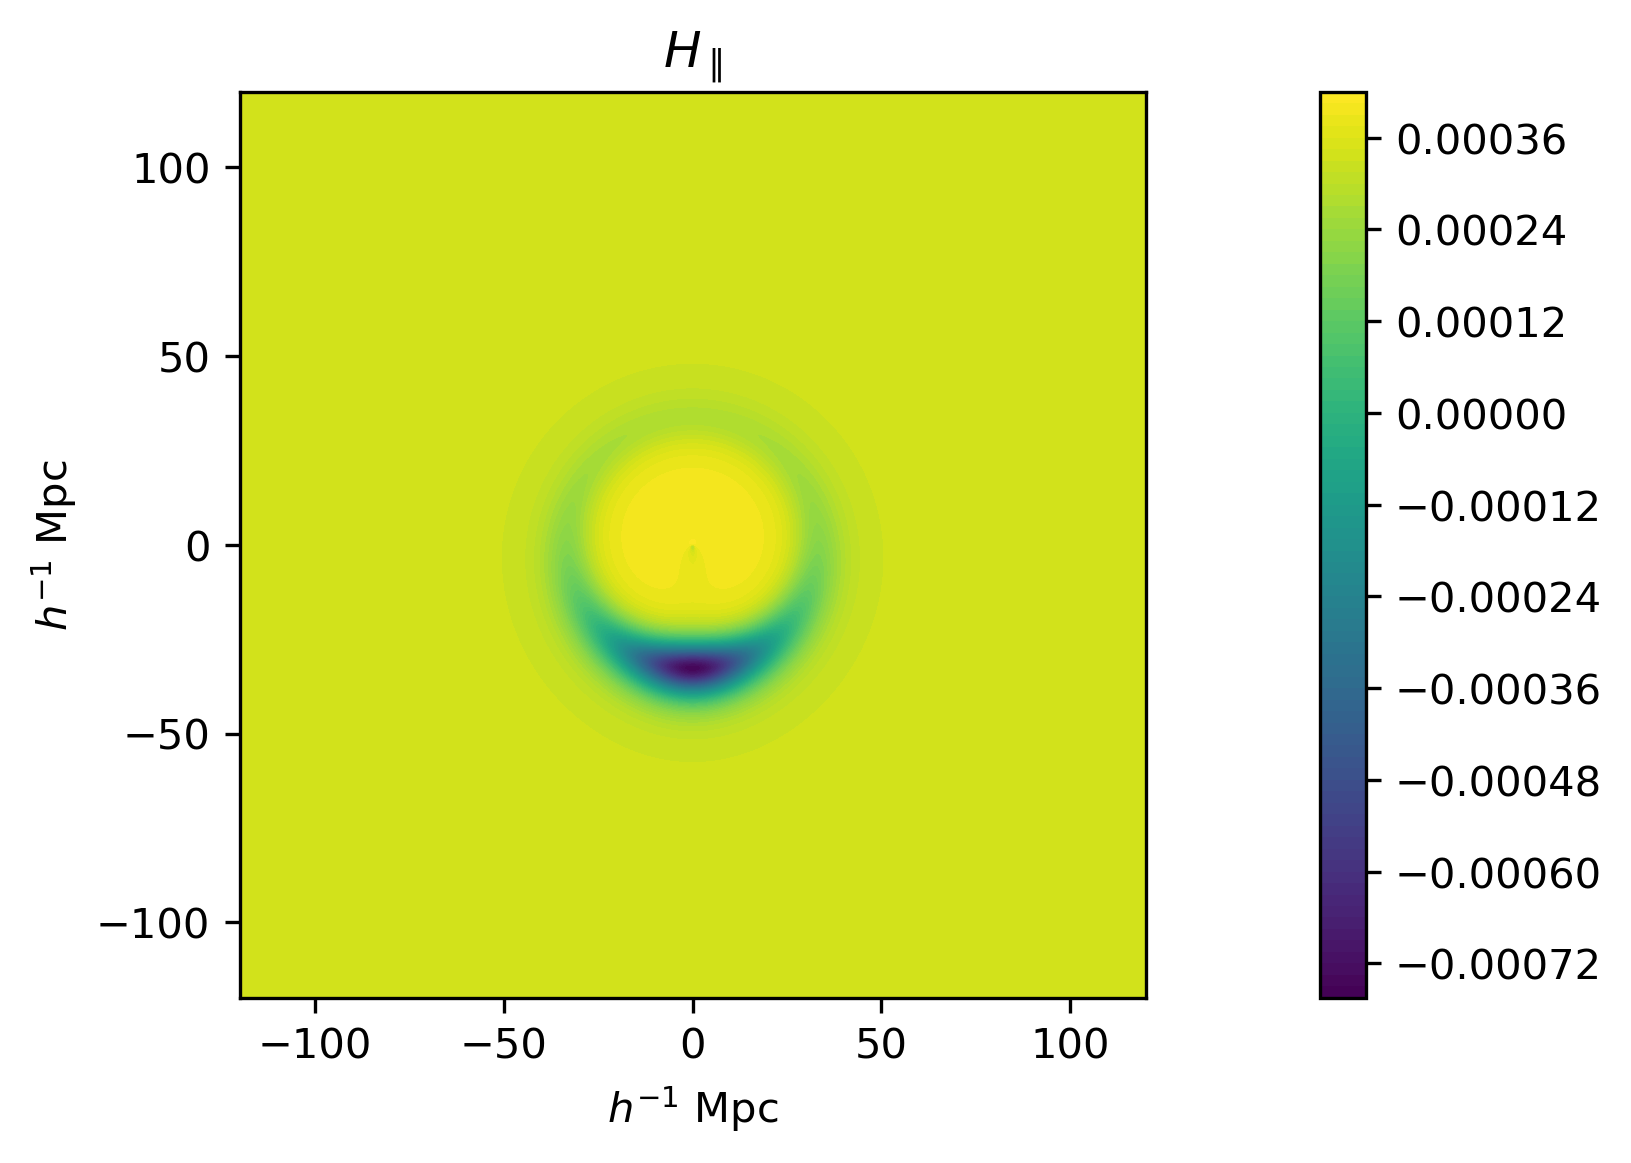
\includegraphics[width=\textwidth]{H_para_example.png}
          \subcaption{}
      \end{subfigure}
      \hfill
      \begin{subfigure}[b]{0.45\textwidth}
          \centering
          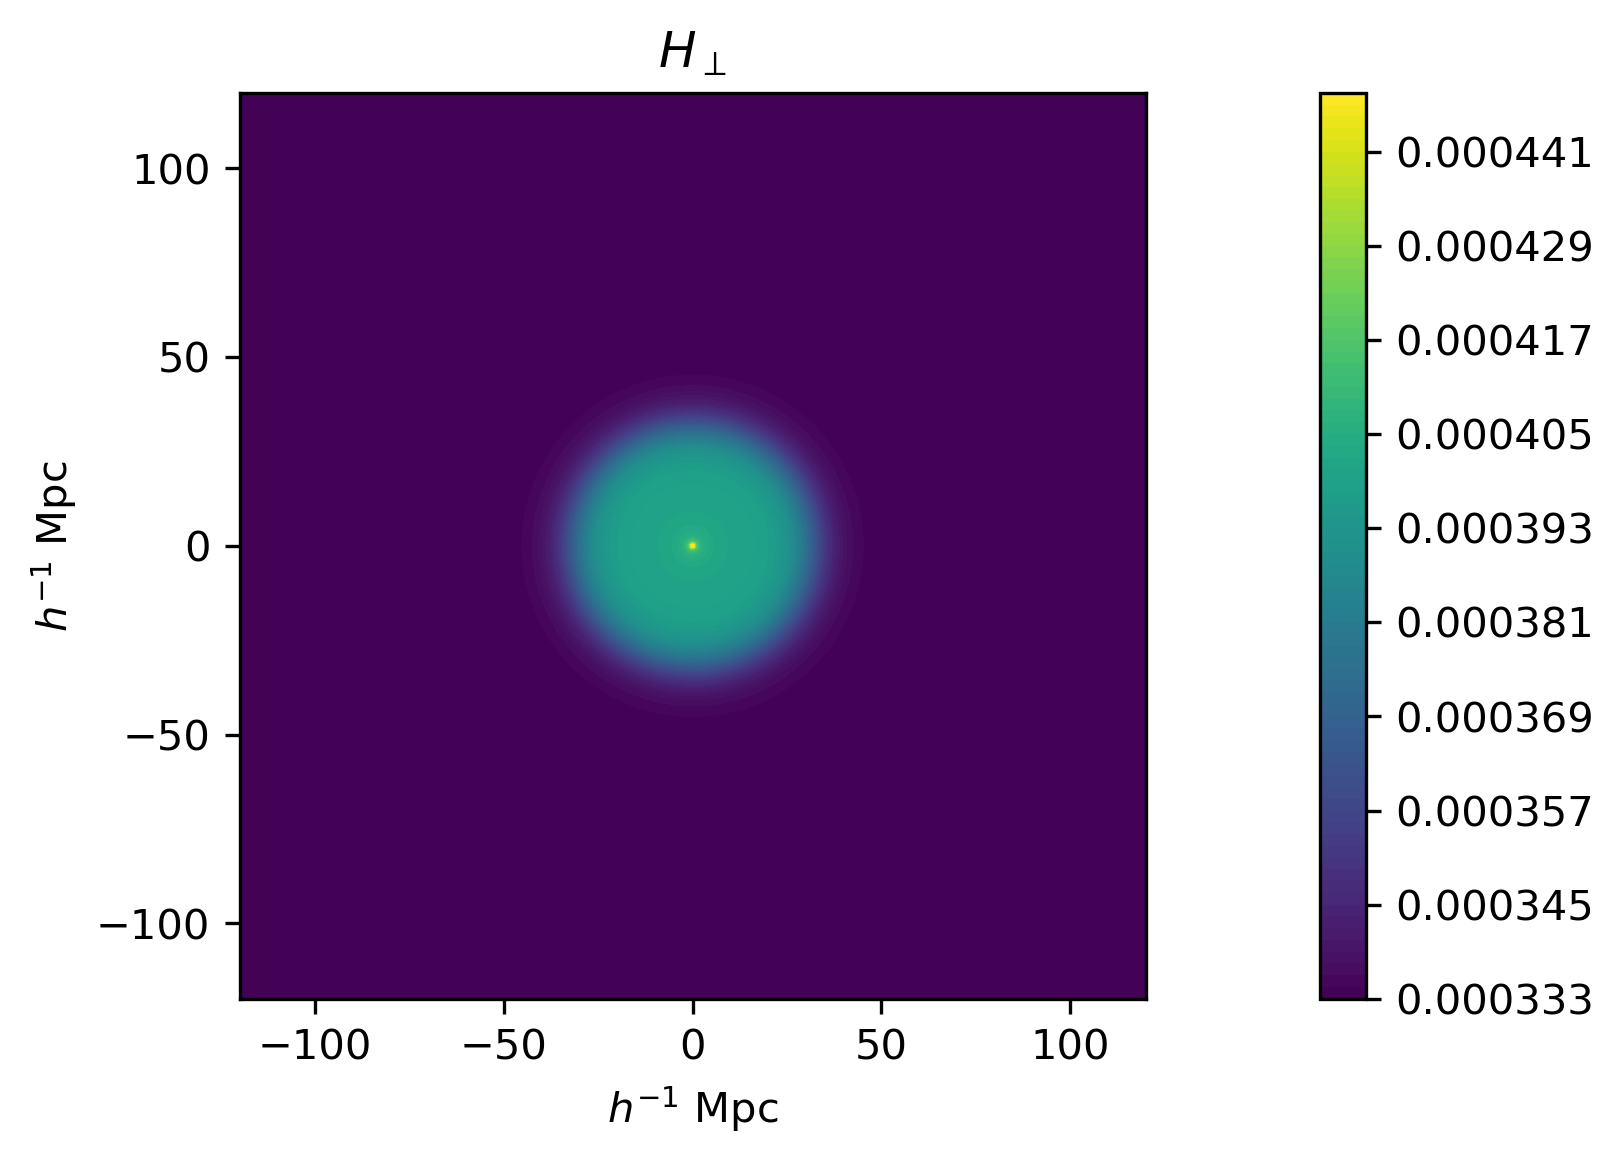
\includegraphics[width=\textwidth]{H_perp_example.png}
          \subcaption{}
      \end{subfigure}

      \caption{Plots along a cross-section of a Szekeres model showing, (a): The density contrast, (b): the expansion scalar $\theta$, (c): the longitudinal expansion $H_\parallel$ =, (d): the transverse expansion $H_\perp$. The geometry is an axisymmetric BNW model where $S'\neq0=P=Q$ (see Section \ref{chapter: BNW model analysis}).}
      \label{fig: szekeres - expansion plot}
\end{figure}
The trace-free symmetric part $\sigma_{\mu\nu}$ is called the shear, and represents a distortion in the shape of the geodesic congruence. In projective coordinates,
\begin{equation}
  {\sigma^\mu}_\nu = \frac{1}{3}(H_\parallel - H_\perp)\,\text{diag}\,(0,2,-1,-1).
\end{equation}
Lastly, the antisymmetric part $\omega_{\mu\nu}$ is called the rotation or vorticity. In Szekeres models this vanishes, so Szekeres models are ``irrotational''. This places a restriction on what we can model, as we cannot model virialized structures, such as a galaxy supported from collapse by the rotational motion of its stars.

For comparison, in an FLRW model the expansion rate of space is homogeneous and isotropic. The expansion scalar is related to the Hubble parameter by,
\begin{equation}
  \theta \equiv {U^{\alpha}}_{;\alpha} = 3H(t),
\end{equation}
and both the shear and rotation vanish.

\section{Physical Equivalence and Coordinate Transformations}
Given two Szekeres models, a natural question to ask is whether they are physically equivalent. As previously stated, a new radial coordinate can be defined using the gauge freedom $r \to \tilde{r} = f(r)$ while retaining the form of the metric. One can also perform a coordinate transformation, then define new dipole functions to return the metric to the form (\ref{eqn: szekeres - proj coords metric}). As one can transform between these two metrics with a coordinate transformation, they are physically equivalent. Overall, these transformations consisting of a coordinate transform and a parametrization take the form
\begin{align}
  (p,q) \to (\tilde{p},\tilde{q}), \\
  (S,P,Q) \to (\tilde{S},\tilde{P},\tilde{Q}).
\end{align}
Georg and Hellaby \cite{RN8} completed a list of such transformations from \cite{RN73}. These transformations are as follows:

\subsubsection{Translation}
\begin{align}
  (\tilde{p},\tilde{q}) &= (p + p_0, q+q_0),\\
  (\tilde{S},\tilde{P},\tilde{Q}) &= (S, P+p_0, Q+q_0). \label{eqn: translation dipole function transformation}
\end{align}
This simply translates the projection point seen in Figure \ref{fig: szekeres - stereographic projection}. The spherical polar coordinates are unchanged.

\subsubsection{Scaling}
\begin{align}
  (\tilde{p},\tilde{q}) &= \mu(p, q),\\
  (\tilde{S},\tilde{P},\tilde{Q}) &= \mu(S, P, Q). \label{eqn: scaling dipole function transformation}
\end{align}
Again, this only affects the stereographic projection, and the spherical polar coordinates are unchanged.

\subsubsection{Polar Rotation}
\begin{align}
  (\tilde{p},\tilde{q}) &= (p\cos(\psi)+q\sin(\psi), -p\sin(\psi)+q\cos(\psi)),\\
  (\tilde{S},\tilde{P},\tilde{Q}) &= (S, P\cos(\psi)+Q\sin(\psi), -P\sin(\psi)+Q\cos(\psi)). \label{eqn: polar rotation dipole functions}
\end{align}
In spherical polar coordinates, this takes the form of a rotation about $\theta=0$, i.e., $\phi \to \tilde{\phi} = \phi+\psi$, and $\theta \to \tilde{\theta}=\theta$.

\subsubsection{Inversion}
\begin{align}
  (\tilde{p},\tilde{q}) &= \frac{(p, q)}{p^2 + q^2},\\
  (\tilde{S},\tilde{P},\tilde{Q}) &= \frac{(S, P, Q)}{S^2 + P^2 + Q^2}.
\end{align}
This is effectively a reflection across the great circle
\begin{equation}
  Px + Qy + Sz = 0
\end{equation}
in terms of the LRF (\ref{eqn: szekeres - LRF definition}). This transformation is particularly useful for dealing with coordinate singularities at the projection point. For example, when solving the geodesic equations the geodesic may approach the projection point, causing $(p,q)$ to blow up. One could perform an inversion to lower $(p,q)$ and move the discontinuity to the opposite side of the shell, avoiding problems with computational precision.

\subsubsection{Haantjes Transformation}
The coordinates transform as
\begin{subequations}  \label{eqn: haantjes transformation - coordinates}
    \begin{align}
      \tilde{p} &= \frac{p + D_1 (p^2 + q^2)}{\tau}\\
      \tilde{q} &= \frac{q+D_2(p^2+q^2)}{\tau},
    \end{align}
\end{subequations}
where
\begin{equation}
  \tau = 1+2D_1p+2D_2q+(D_1^2+D_2^2)(p^2+q^2).
\end{equation}
The new dipole functions are then
\begin{subequations}\label{eqn: Haantjes tranform dipole functions}
    \begin{align}
      \tilde{S} &= \frac{S}{T}, \\
      \tilde{P} &= \frac{P + D_1 (S^2+P^2 + Q^2)}{T},\\
      \tilde{Q} &= \frac{Q+D_2(S^2+P^2+Q^2)}{T},
    \end{align}
\end{subequations}
where
\begin{equation}
  T = 1+2D_1P+2D_2Q+(D_1^2+D_2^2)(S^2+P^2+Q^2).
\end{equation}
This is also known as an equatorial rotation, and is effectively a rotation in an arbitrary direction. A Haantjes transformation is equivalent to an inversion, followed by a translation by $(D_1,D_2)$, then another inversion.

This transformation is particularly useful in constructing models. One can rotate an anisotropy to a desired direction whilst retaining the alignment of other structure. This is done by applying a Haantjes transformation to only the subset of the shells where the anisotropy to be rotated is. Since this transformation is done locally and not globally, this does not give a physically equivalent model. Applying this to a number of anisotropies at different radii gives an ``onion'' model \cite{RN1}.

\subsection{Symmetry}
On the subject of physical equivalence, under certain conditions on the dipole functions the Szekeres geometries can possess a symmetry. Choosing constant $S$, $P$, and $Q$ trivially gives isotropy, but under looser conditions one can have axial symmetry or bilateral symmetry. These symmetries are advantageous for model construction, as they can make the mathematics more tractable or reduce computation time when utilised. However, they do restrict the arrangements of structures that can be modelled.

\subsubsection{Axial Symmetry}
In axial symmetry, the geometry has a single Killing vector generating a rotation about an axis of symmetry. One can create a model with axial symmetry by setting $P'=Q'=0$, i.e., having $S$ be the only non-constant dipole function. In this case, the axis of symmetry is along the line $\theta=0$ and $\theta = \pi$. Models with the axis of symmetry in different directions will appear more complicated due to the effects of shell shifting and rotation. However, it turns out that all axisymmetric solutions can be related to a solution with $P'=Q'=0$ by a Haantjes transformation \cite{RN8}. This is great news for model construction. If we want an axisymmetric model, we can set $P'=Q'=0$ to get a mathematically simpler model without restricting the physical geometries available to us.

The axis of symmetry lies on the line of constant projective coordinates $(p_0,q_0)$ (and its antipodal point) for all $r$, and satisfies the conditions,
\begin{align}
  \mathcal{E}\mathcal{E}_{,pr} &= \mathcal{E}_{,p} \mathcal{E}_{,r}, & \mathcal{E}\mathcal{E}_{,qr} &= \mathcal{E}_{,q} \mathcal{E}_{,r},
\end{align}
along the axis of symmetry \cite{RN8,RN4,RN1}. When generated using a Hanntjes transformation, the coordinates of the axis of symmetry are $(0,0)$ and
\begin{equation}
    (p_0, q_0) = \frac{(D_1, D_2)}{D_1^2 + D_2^2}.
\end{equation}

Axisymmetric models are convenient for the type of investigation conducted in this thesis, where we are simulating an observer's measurements by using ray tracing. The symmetry allows one to restrict observers to lie on a half-plane without loss of generality, effectively removing a coordinate from investigation. However, they have limited application when constructing realistic models with more than one structure, as the density extrema are all restricted to lying on the axis of symmetry.

\subsubsection{Bilateral Symmetry}
Szekeres solutions can also possess bilateral symmetry, where the geometry is invariant to reflections across a symmetry plane passing through the origin. The extrema of $\mathcal{E}'/\mathcal{E}$ then all lie in this symmetry plane, and thus the direction of shell shifting, shell rotation, and density extrema are also located on this plane. Thus, Szekeres models with bilateral symmetry can be accurately represented by 2D plots taken on this symmetry plane.

Two simple examples are when $P'=0$, in which case the symmetry plane is $\phi=\pm \pi/2$ with $\theta$ free; and $Q'=0$, in which case the symmetry plane is $\phi = \{0,\pi\}$ with $\theta$ free. One could then rotate the symmetry plane to an arbitrary direction with a Haantjes transformation. However, not all bilaterally symmetric models can be constructed this way. See \cite{RN1} for a more thorough discussion of bilateral symmetry.

Bilateral symmetry loses much of the convenience of axisymmetric models, as one cannot remove a whole coordinate from investigation. However, in certain circumstances it can divide the number of directions to be considered in half. For example, one can restrict observers to lying on one half of the plane without loss of generalisation. Furthermore, if an observer is on the symmetry plane, one only needs to perform ray tracing on one half of their sky. In exchange for this loss of convenience compared to axially symmetric Szekeres models, we gain some generality in the models we can construct. A bilaterally symmetric model can accurately represent systems with up to two structures. However, for three or more structures, we lose some realism due to the constrained positions of the structures.


\section{Plotting Constant-\textit{t} Slices} \label{section: szekeres - plotting}
To generate plots of a Szekeres model, we need to map the geometry onto a flat 2D plane. As the Szekeres models have non-negligible curvature, any such projection will introduce distortion. For this thesis, we mainly use the scheme described by Buckley and Schlegel \cite{RN1} (B\&S). Broadly speaking, we first calculate the effects of shell shifting and rotation, then use these results to project the constant-$t$ geometry into 3D Euclidean a space. In this space, we can select a representative 2D subspace to plot.

\subsection{Calculating Shell Shifting and Rotation}
B\&S track the shell rotation and shell shifting of shell $r$ at time $t$ using a $3 \times 3$ matrix $A(r)$, and a displacement vector $\bm{\Delta}(t,r)$. The matrix $A(r)$ represents the rotation of the shell's LRF with respect to the innermost shells, and $\bm{\Delta}(t,r)$ is the total displacement of the shell. These are generated numerically, starting at $r=0$ with $A(r)=I_3$ and $\bm{\Delta}(t,0)=\vec{0}$ and incrementing in small steps $\delta r$ up to a maximum $r_\text{max}$. At each step, $A$ is updated by
\begin{equation} \label{eqn: szekeres - shell rotation matrix update}
  A(r+\delta r) = R_y\left(\frac{P'}{S}\delta r\right)R_x\left(-\frac{Q'}{S}\delta r\right)A(r),
\end{equation}
and $\bm{\Delta}$ is updated by
\begin{equation} \label{eqn: szekeres - shell shift vector update}
  \bm{\Delta}(t,r+\delta r) = \bm{\Delta}(t,r) + \frac{R(t,r)}{\sqrt{1-k(r)}}A^T(r)\begin{bmatrix}
    P'/S \\ Q'/S \\ S'/S
\end{bmatrix}(r) \delta r.
\end{equation}
In \eqref{\ref{eqn: szekeres - shell rotation matrix update}}, $R_x$ and $R_y$ are rotation matrices about the $x$ and $y$ directions respectively in the LRF. Since the angles are small, they approximately commute. These rotation matrices are given by
\begin{subequations}
\begin{align}
  R_x(\psi) &=
  \begin{bmatrix}
    1 & 0 & 0\\
    0 & \cos(\psi) & -\sin(\psi)\\
    0 & \sin(\psi) & \cos(\psi)
    \end{bmatrix},\\
  R_y(\psi) &=
  \begin{bmatrix}
    \cos(\psi) & 0 & \sin(\psi)\\
    0 & 1 & 0\\
    -\sin(\psi) & 0 & \cos(\psi)
  \end{bmatrix}.
\end{align}
\end{subequations}

The values of $A(r)$ and $\bm{\Delta}(t,r)$ are stored in an array to keep track of their value at each $r$. When applying this procedure for plotting, we set $k(r)=0$ within (\ref{eqn: szekeres - shell shift vector update}). Note that evaluating $\bm{\Delta}$ at different times requires a recalculation of the above procedure, but $A(r)$ does not have this same time dependence.

\subsection{Projection onto Euclidean Space}
We project the polar coordinates $r,\theta,\phi$ at time $t$ onto a 3D Euclidean space using the following,
\begin{equation} \label{eqn: szekeres - projection to cartesian}
  \begin{bmatrix}
    X \\ Y \\ Z
  \end{bmatrix}
  = R(t,r)A^T(r)
  \begin{bmatrix}
    \sin(\theta)\cos(\phi) \\ \sin(\theta)\sin(\phi) \\ \cos(\theta)
  \end{bmatrix}
  + \bm{\Delta}(t,r),
\end{equation}
where we have used $k(r)=0$ when calculating the shell rotation and shift to remove the curvature. This projection accurately conveys distances along the shell's surface, but distorts distances between shells.

An alternative projection suggested by B\&S which includes the effects of $k(r)$ is to replace $R(t,r)$ in (\ref{eqn: szekeres - projection to cartesian}) with $R_{map}(t,r)$, defined by
\begin{equation}
  R_{map}(t,r) = \int_0^r \frac{R'(t,\tilde{r})}{\sqrt{1-k(\tilde{r})}}\diff{\tilde{r}},
\end{equation}
and to include the curvature factor when calculating the shell shifting. This projection accurately conveys distances along lines of constant projective coordinates $(p,q)$, but distorts sizes of shells and distances along their surfaces. In the models considered in this thesis, $k(r)$ is small, so these projections give almost the same result. This can be seen in Figure \ref{fig: szekeres - projection examples}.
\begin{figure}[!tbh]
     \centering
     \begin{subfigure}[b]{0.45\textwidth}
         \centering
         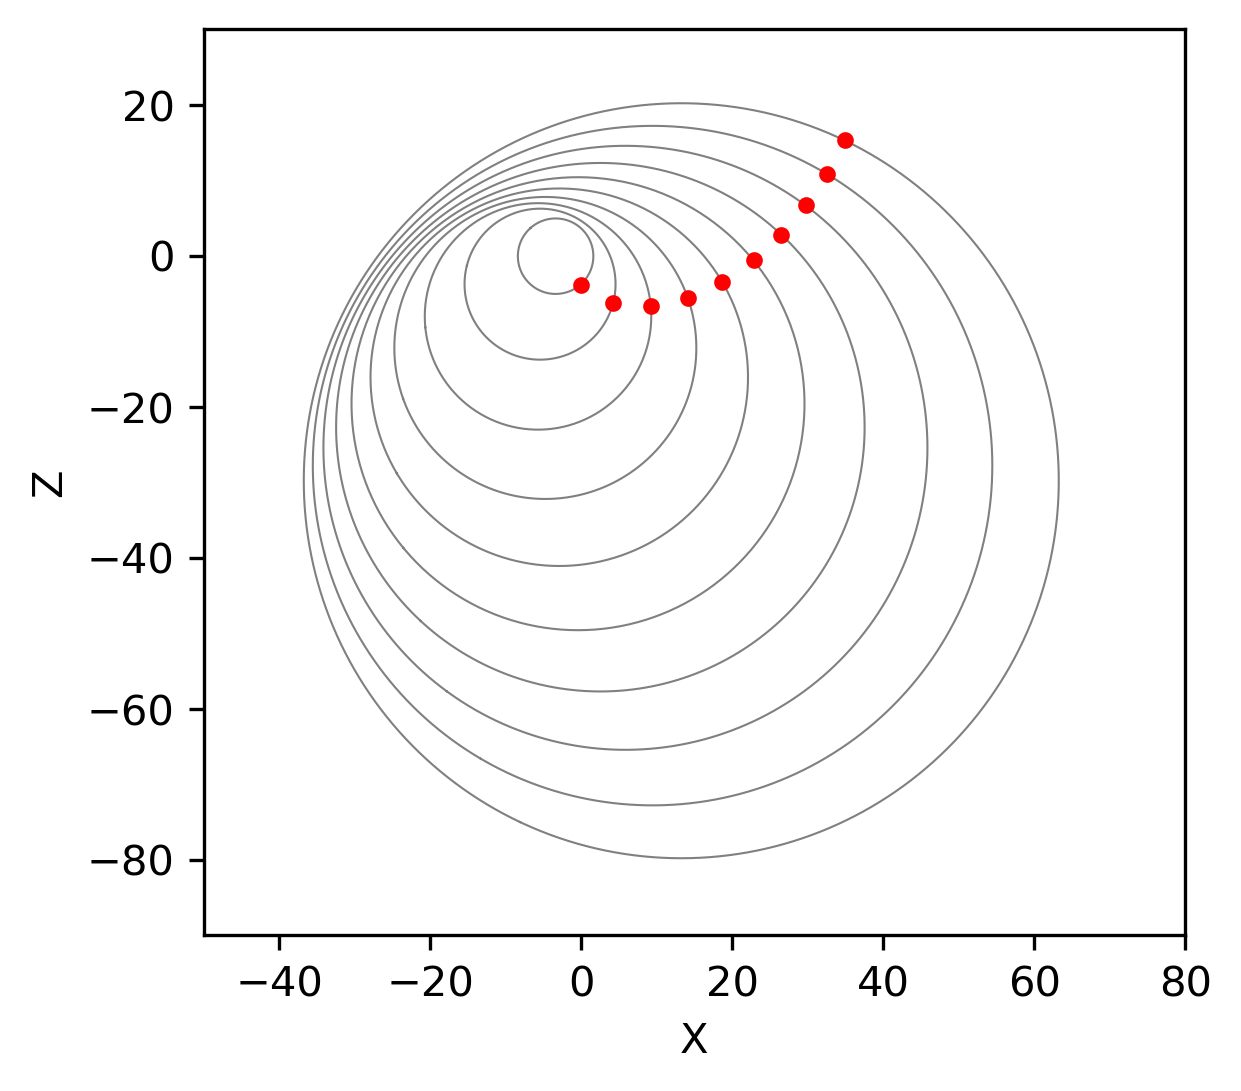
\includegraphics[width=\textwidth]{example plot no curvature.png}
     \end{subfigure}
     \hfill
     \begin{subfigure}[b]{0.45\textwidth}
         \centering
         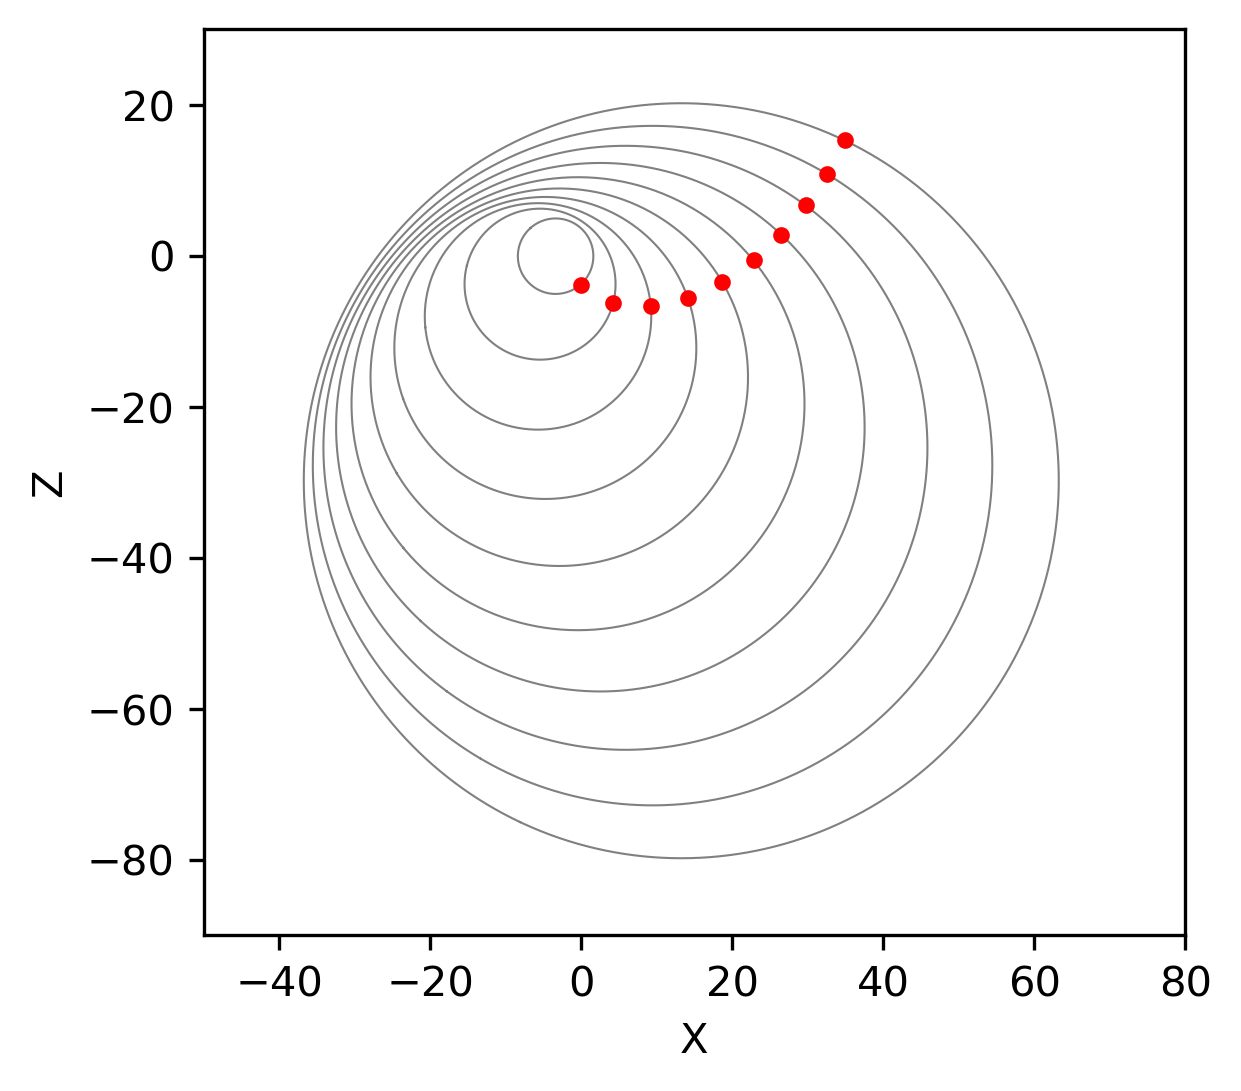
\includegraphics[width=\textwidth]{example plot curvature.png}
     \end{subfigure}
      \caption{Example plots of cross-sections of the shells $\phi=0, r=5,10, ... , 50$ using each projection method. Both plots use a model where the dipole functions are $S(r)=1$, $P(r)=\alpha\log(1+r)$, and $Q(r)=0$. On the left is the first method described, neglecting the effects of $k(r)$. On the right is the second method described, including $k(r)$. The red dots signify the points $\theta=0$.}
      \label{fig: szekeres - projection examples}
\end{figure}

From here, we can select a 2D subspace to generate our plot. If the model has some symmetry, there may be a convenient choice of this subspace. For an axially symmetric model, one could select a plane containing the axis of symmetry. For example, the model with $P'=Q'=0$ and $S' \neq 0$ is axially symmetric, with the axis of symmetry running through $\theta=0$ and $\theta = \pi$. In the projection methods outlined above, the axis of symmetry is projected onto the $Z$-axis, so plotting the $(X,Z)$ or $(Y,Z)$ plane gives a representative plot. For a bilaterally symmetric geometry, the plane of symmetry gives a representative plot. For example, for a model where $Q'=0\neq P'$ the plane of symmetry is $\phi=\{0,\pi\}$, and when projected into 3D Euclidean space this corresponds to plotting the $(X,Z)$ plane.



%%%%%%%%%%%%%%%%%%%%%%%%%%%%%%%%%%%%%%%%%%%%%%%%%%%%%%%%%%%%%%%%%%%%%%%%%%%%%%%%
\chapter{Ray tracing and Re-analysis of the Axisymmetric Model} \label{chapter: BNW model analysis}
%%%%%%%%%%%%%%%%%%%%%%%%%%%%%%%%%%%%%%%%%%%%%%%%%%%%%%%%%%%%%%%%%%%%%%%%%%%%%%%%
In this chapter, we outline the methods used to simulate observables in Szekeres models, and analyse the axisymmetric Szekeres model used by Bolejko, Nazer, and Wiltshire in their 2016 paper \cite{RN3} (BNW). The goal of this analysis is to determine a good fit to the large angle Hubble anisotropy in the COMPOSITE catalogue and to the observed CMB dipole and quadrupole without the use of a bulk flow.

The BNW model simulates spacetime on the intermediate scale of tens of megaparsecs. At this scale, it still makes sense to smooth over the density fluctuations within galaxies and galaxy clusters, and approximate the matter as an average fluid. However, this averaged fluid will contain inhomogeneities. We are known to be within a void which is surrounded with over-densities such as the Virgo cluster, the Perseus-Pisces Supercluster, and the Great Attractor \cite{RN168}. To examine the non-linear effect on light propagation from this nearby structure in a toy Szekeres model, the BNW model contains a void with a single neighbouring overdense structure.

The simulations are performed using Fortran code. This code numerically solves the model dynamics to obtain $k(r)$ and $R(t,r)$, then, performs ray tracing to create a simulated COMPOSITE catalogue and CMB measurement. This code utilises the HEALPix (Hierarchical Equal Area isoLatitude Pixelisation) libraries for sphere discretisation and spherical harmonic analysis\footnote{See \url{https://healpix.sourceforge.io/}.} \cite{RN250}. The Fortran code which creates these simulated measurements is packaged into a Python library using \texttt{f2py} \cite{RN112}, and is used with the Python library \texttt{emcee} \cite{RN113,RN111} to implement a Markov Chain Monte Carlo (MCMC) method to obtain fitting information.

BNW \cite{RN3} conducted a grid search over the parameter space of the BNW model, and found a set of parameters which matched the amplitude of the CMB dipole and the Hubble expansion dipole in the COMPOSITE catalogue. Unfortunately, their simulation code was later found to contain a bug in the 4-vector initialisation scheme \cite{RN6,RN42}. Therefore, in this chapter, we will perform simulations and explore parameter space with the aim of finding a well fitting parameter set using independently developed code.


\section{The Axisymmetric BNW Model} \label{section: BNW model description}
For this initial investigation, we use the Szekeres model introduced by BNW \cite{RN3}, and used by Dam \cite{RN6} and Hills \cite{RN42}. This geometry models a void with a neighbouring overdensity. The gauge freedom of the $r$ coordinate is used to set $R(t_0,r)=r$. The effective gravitational mass function $M$ is set to
\begin{equation}\label{eqn: BNW M(r) form}
  M(r) = M_0 r^3 \left[1 + \delta_M(r)\right],
\end{equation}
where
\begin{align}
  \delta_M(r) &= \frac{1}{2}\delta_0\left[1 - \tanh\left(\frac{r-r_0}{2\Delta r}\right)\right], &
  M_0 &= \frac{1}{2}H_0^2 \Omega_{m0},
\end{align}
the parameter $\delta_0$ gives the density contrast at the centre of the void, $r_0$ gives the radius of the void in comoving coordinates, and $\Delta r$ affects the rate at which the density contrast changes from $\delta_0$ to $0$. As we wish to model a void, we constrain $\delta_0$ to the range $-1 \leq \delta_0 \leq 0$.
We set $t_B(r)=0$ to get a simultaneous Big Bang, matching observations of near homogeneity in the CMB. These choices fix $k(r)$ through \eqref{\ref{eqn: bang time integral}}, and as $t_B(r)  = 0$ and $M(r) < M_0 r^3$ it can be shown that $k(r) < 0$. A proof of this is presented in Appendix \ref{appendix: k <= 0 proof}. An example solution of $k(r)$ and $R(t,r)$ for this model is presented in Figure \ref{fig: BNW dynamics example plots}.

\begin{figure}[ht]
     \centering
     \begin{subfigure}[b]{0.45\textwidth}
         \centering
         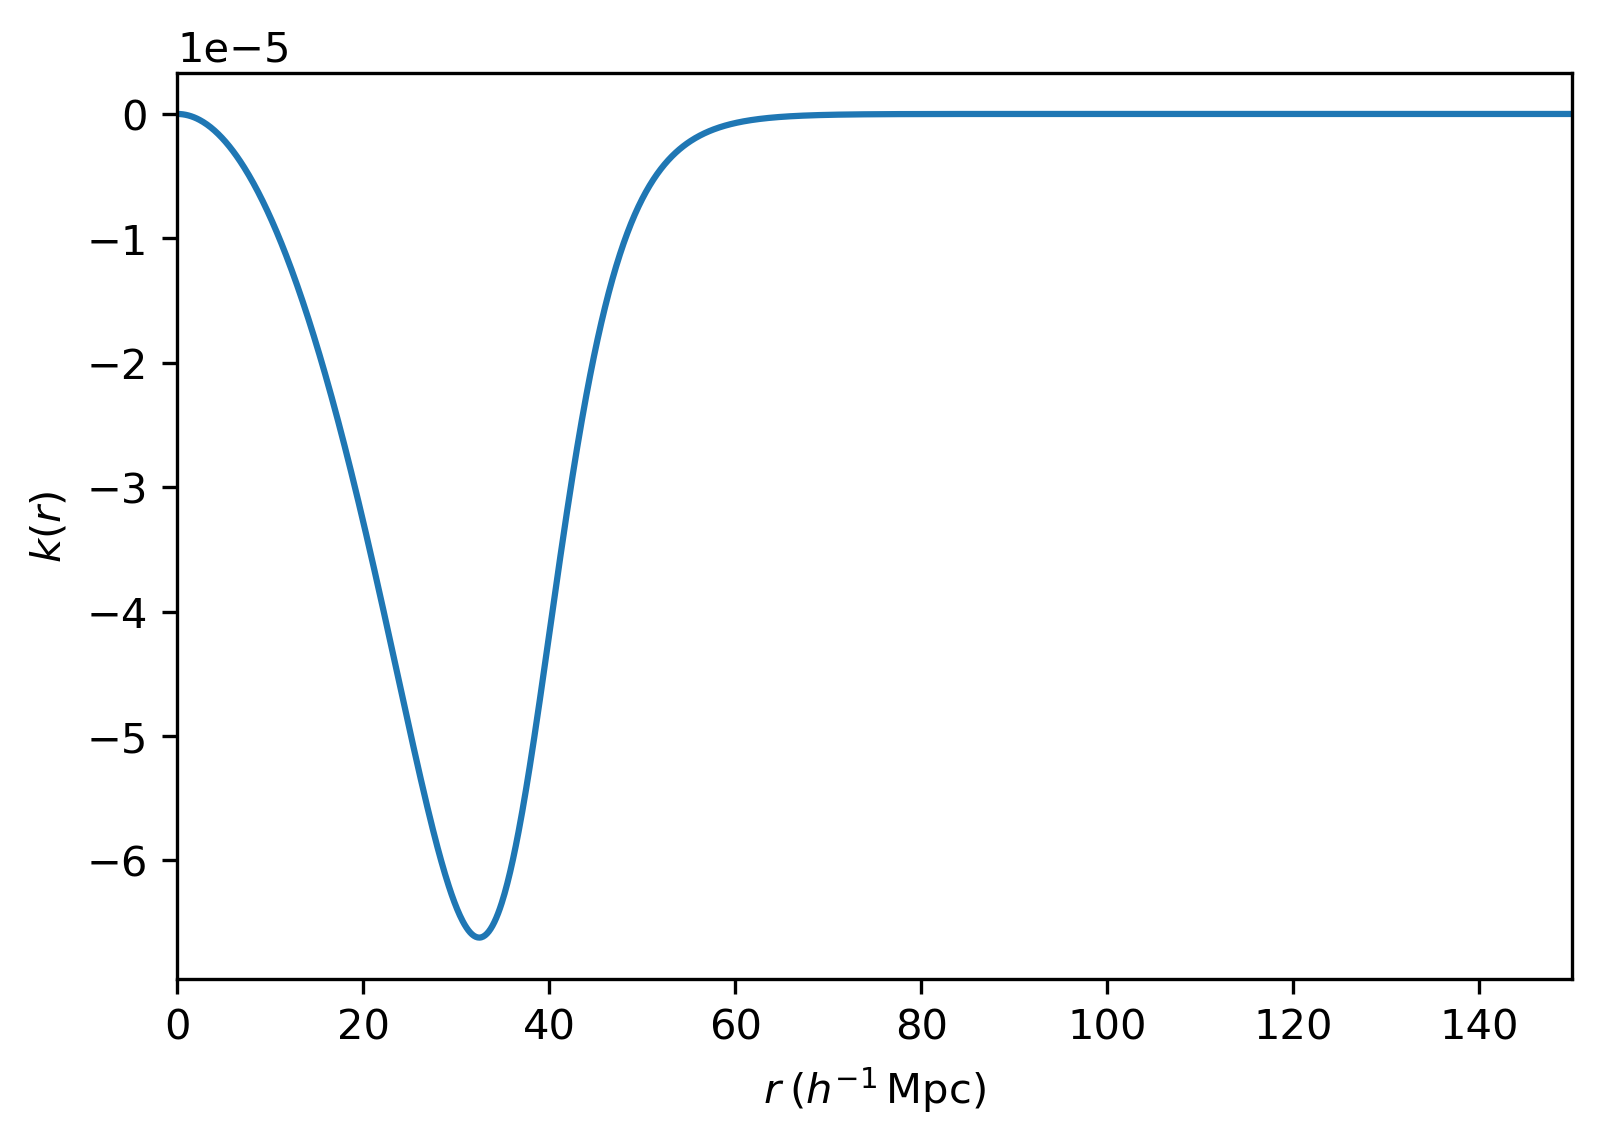
\includegraphics[width=\textwidth]{BNW params k_plot.png}
     \end{subfigure}
     \begin{subfigure}[b]{0.45\textwidth}
         \centering
         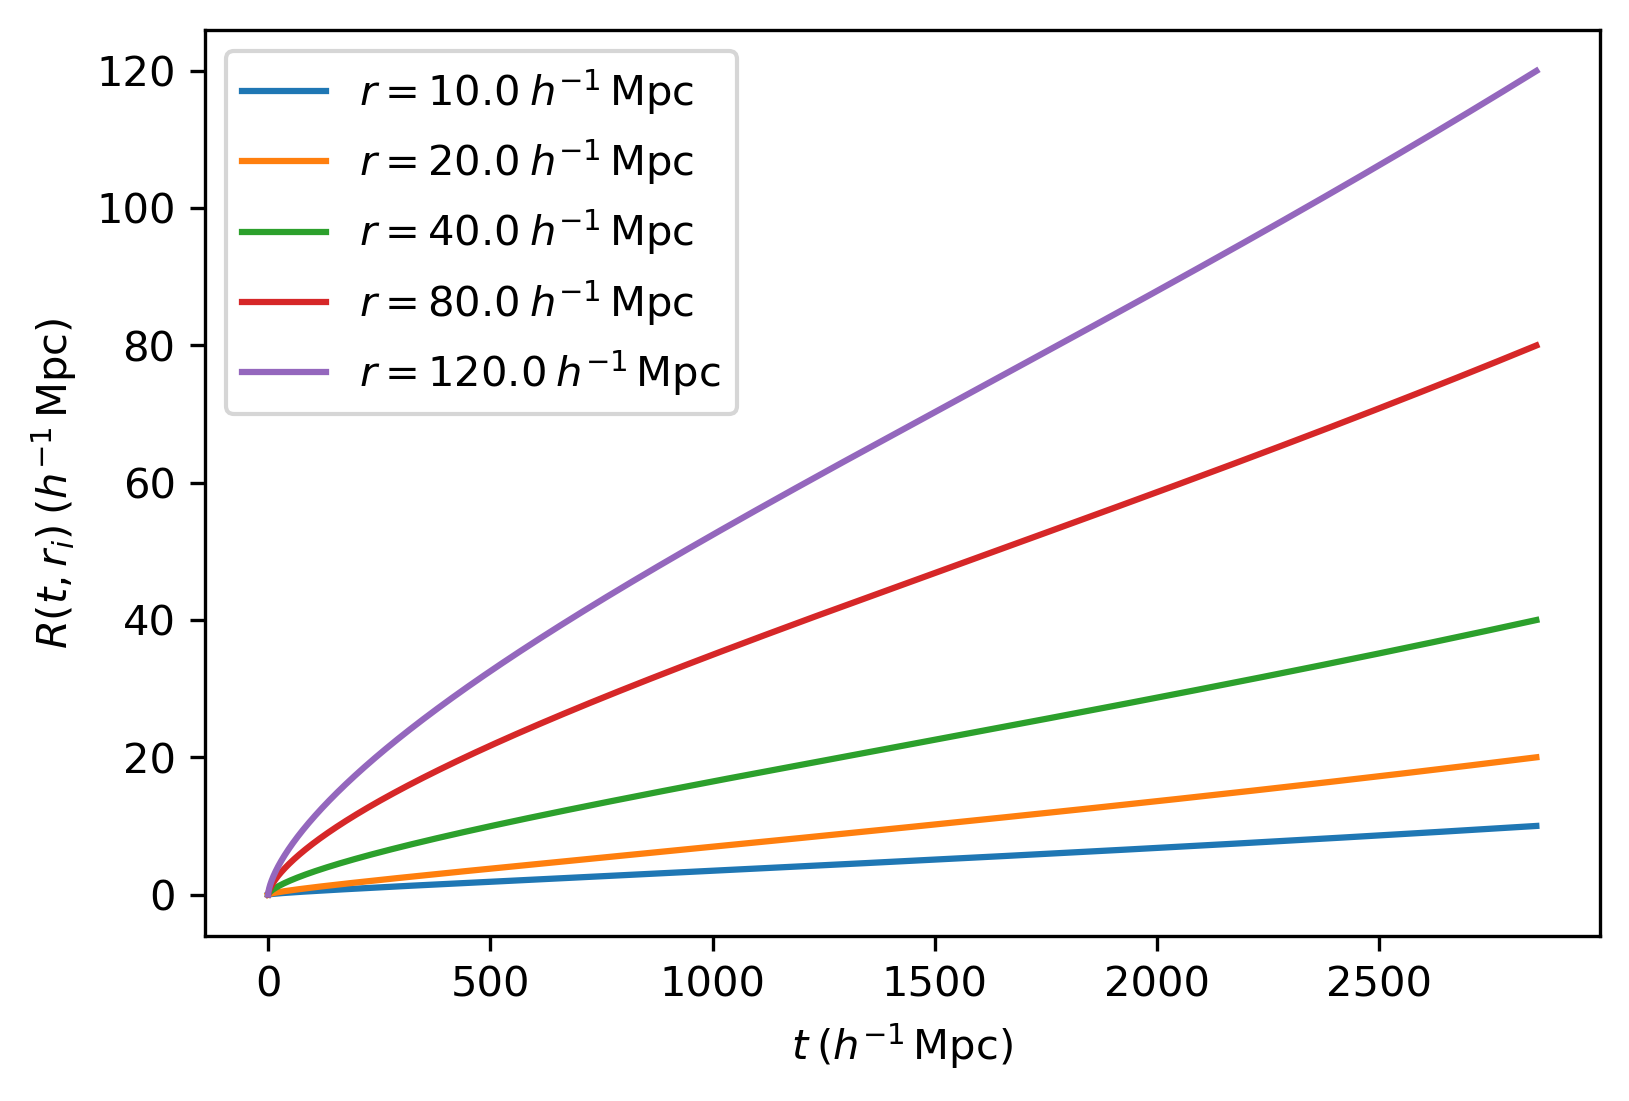
\includegraphics[width=\textwidth]{BNW params R_plot.png}
     \end{subfigure}
      \caption{Example plots of $k(r)$ (left) and $R(t,r)$ (right). The left plot shows $k(r)$ from $r=0$ to $r=150\, h^{-1}\,$Mpc. For small values of $r$, the geometry is similar to a curved FLRW model, so $k(r) \propto r^2$. At large values of $r$, the geometry is well approximated by a spatially flat FLRW model, so $k(r) \approx 0$. The right plot shows $R(t,r)$ at increasing $r$ values as the coordinate time varies from $t=0$ to the present coordinate time, $t=t_0=2854\, h^{-1}\,$ Mpc. The coordinate $t$ is measured in $h^{-1}\,$Mpc because we have chosen units where $c=1$. Note at $t=0$ the solutions all converge to $R(0,r)=0$, this is indicative of the simultaneous bang time set by $t_B(r)=0$. These plots use the canonical BNW model, which has the parameters seen in \eqref{\ref{eqn: canonical BNW model parameters}}.}
      \label{fig: BNW dynamics example plots}
\end{figure}

The dipole functions are set to
\begin{align}
  S(r) &= \left(\frac{r}{1\, h^{-1}\, \text{Mpc}}\right)^\alpha, \\
  P(r) &= Q(r) = 0.
\end{align}
Since $S' \neq 0$ and $P'=Q'=0$, this geometry is axially symmetric with an axis of symmetry through $p=q=0$ and the projection point ($\theta=0$ and $\theta=\pi$ in spherical polar coordinates), and the geometry has no shell rotation. With this choice of dipole functions the extrema of $\mathcal{E}'/\mathcal{E}$ are $\pm\alpha/r$, so at $t=t_0$ the denominator of the density equation (\ref{eqn: szekeres - mass density equation}) has extrema of $r^2(1 \mp \alpha)$.
Thus, to have a finite mass density $\alpha$ is restricted to the domain $-1 < \alpha < 1$. The regular origin conditions (\ref{eqn: szekeres - regular origin conditions}) taken at $t=t_0$ further constrain this domain to $0 \leq \alpha < 1$. Note that when $\alpha = 0$ we get an isotropic LTB geometry.

\subsection{Asymptotic Behaviour}
At large $r$, $M(r) \to M_0 r^3$, $k(r) \to 0$, and $R(t,r) \to ra(t)$, so the geometry approaches a flat FLRW limit. With this property in mind, we only solve the dynamics of the Szekeres geometry for $r<400\, h^{-1}\,$Mpc.
For anything further out, a spatially flat FLRW geometry is an accurate approximation, so we use it instead (e.g., \eqref{\ref{eqn: standard model - cosmological redshift}} for redshift). For this FLRW metric, we use the model parameters for the spatially flat $\Lambda$CDM model from Planck \cite{RN32},
\begin{align} \label{eqn: BNW model - FLRW parameters}
  \Omega_{m0} &= 0.315, & \Omega_{\Lambda0} &= 0.685, & \Omega_{k0} &= \Omega_{r0} = 0.
\end{align}
This asymptotic behaviour can be seen in Figure \ref{fig: BNW params density contrast}, which shows a cross-section of the density contrast $\delta_\rho = (\rho-\rho_\text{FLRW})/\rho_\text{FLRW}$ where $\rho_\text{FLRW}$ is the matter density of the FLRW model with parameters (\ref{eqn: BNW model - FLRW parameters}).

\begin{figure}[htb]
  \centering
  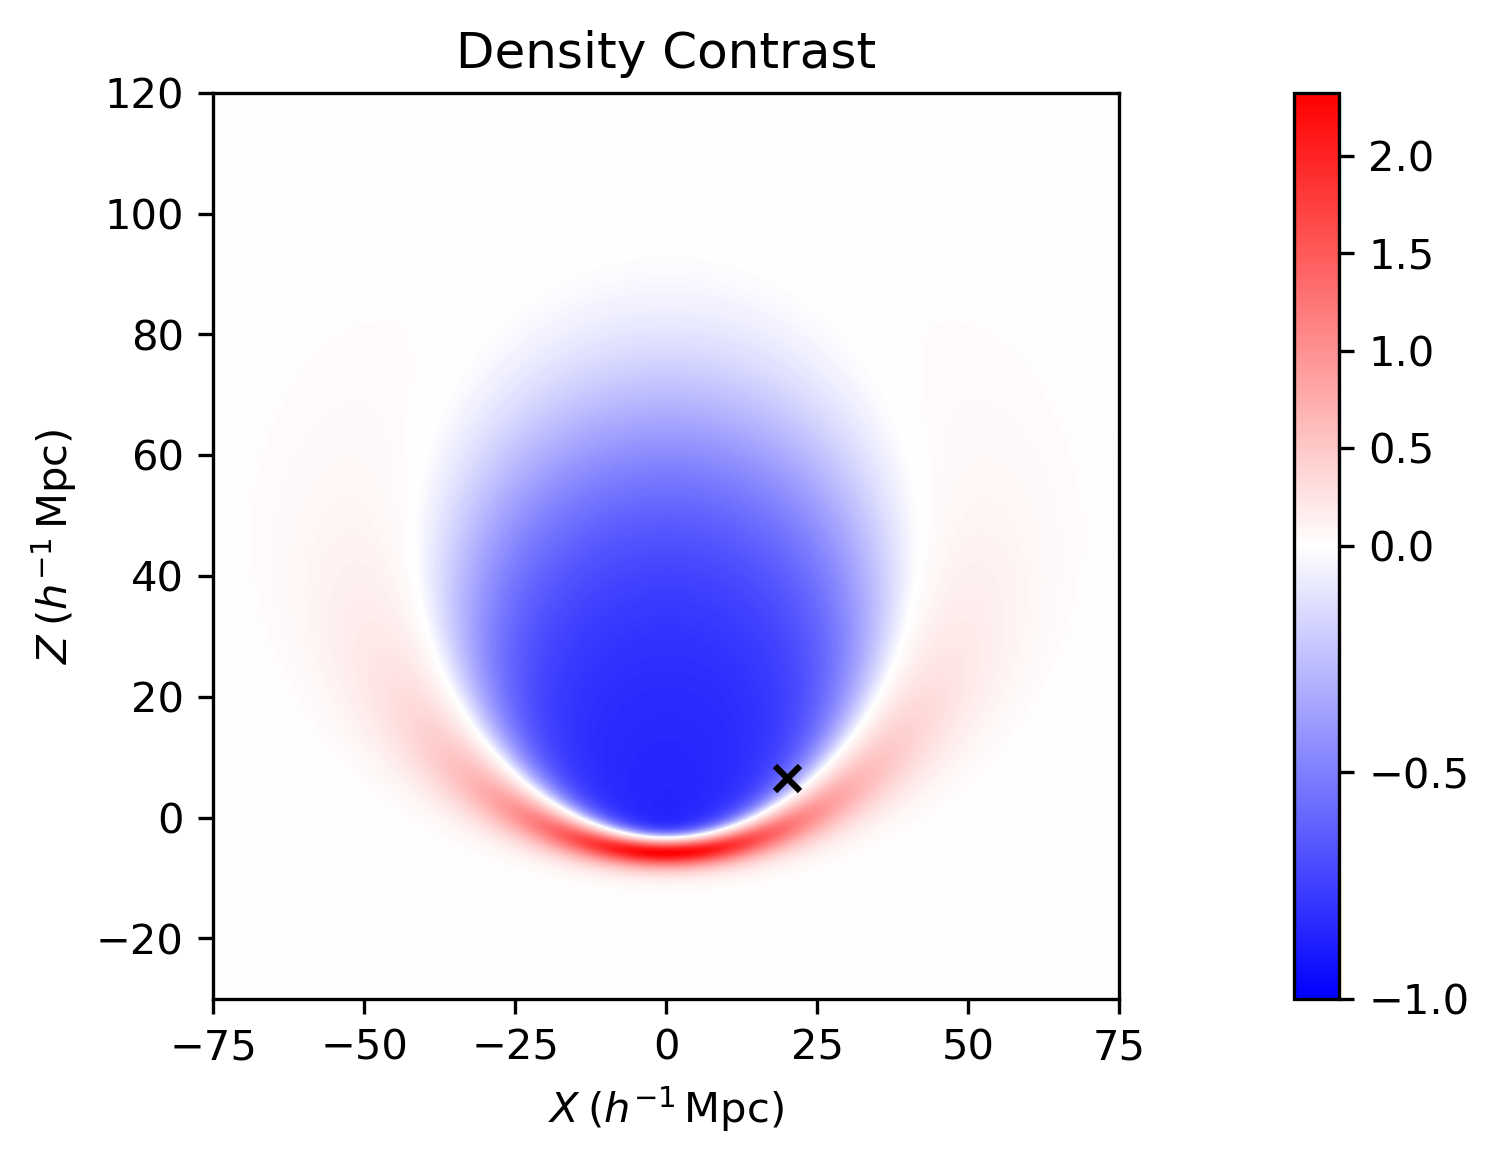
\includegraphics[width=105mm]{BNW params density contrast}
  \caption{The density contrast of the canonical BNW model, which has the parameters seen in \eqref{\ref{eqn: canonical BNW model parameters}}. The black `x' indicates the position of the observer. Note that beyond the initial structure, the density contrast quickly goes to 0, indicating that the density is the same as that of the spatially flat FLRW model with the parameters given in \eqref{\ref{eqn: BNW model - FLRW parameters}}. This is a cross-section taken at $t=t_0$, and $\phi=(0,\,\pi)$. Due to the axial symmetry of the model, the density contrast on this cross-section is the same regardless of the $\phi$ value used. As with all cross-section plots of a Szekeres model in this section, this uses the projection and plotting methods described in Section \ref{section: szekeres - plotting}.}
  \label{fig: BNW params density contrast}
\end{figure}


\section{Simulating the Observables}
For a given set of parameters, we want to calculate the CMB dipole and quadrupole, and the Hubble flow dipole and quadrupole (as seen in Section \ref{section: introduction - hubble flow anisotropy}). There are three steps to this calculating these quantities for a given set of parameters. First, we solve the dynamics of the system to obtain $R(t,r)$ and $k(r)$. Then, we perform ray tracing to simulate a CMB measurement and create a mock COMPOSITE catalogue. Finally, we calculate the desired quantities from these simulated datasets to compare to the observed quantities.

Following the results of \cite{RN35,RN40} and the method of BNW \cite{RN3}, we assume the Local Group frame is the frame of most uniform expansion, and so take it to be comoving in our Szekeres models. Notably, this neglects the possibility of bulk flows, which could significantly affect the simulated Hubble flow \cite{RN122}. We also take our simulated observer to be comoving, therefore all observed data is transformed to the Local Group frame before performing simulations or comparing results. We also assume all sources in the COMPOSITE sample are comoving, that the surface of last scattering has constant coordinate time, and that the primordial plasma at the surface of last scattering is homogenous with a comoving velocity field.

If one were to attempt to perform a rigorous fit of Szekeres models to observations, these restrictions would have to be loosened, e.g., using perturbation theory on a background Szekeres model to obtain a distribution of source velocities. However, a Szekeres model with these restrictions gives a reasonably good toy model to explore the effects of differential expansion without bulk flows.

\subsection{Dynamics of the Systems}
Before performing ray tracing, we need to be able to evaluate $k(r)$ and $R(t,r)$. Unfortunately, these functions cannot be evaluated in terms of familiar functions, as their solutions involve elliptic integrals \cite{RN98}. Instead, we numerically solve for their values on a grid $(t_i, r_j)$ before performing ray tracing, and interpolate between these grid points when needed. The grid used has 5000 points radial coordinates $r_j$ between $r=0$ and $r=500$, and uses 10,000 points time coordinates $t_i$ between $t=t_0$ and $t=0$.

To find $k(r_j)$, we numerically solve \eqref{\ref{eqn: bang time integral}} evaluated at the current time at each radial grid point, i.e.,
\begin{equation}\label{eqn: present time bang time t_B = 0}
  t_0 = \int_0^{r_j} \frac{\diff{\tilde{R}}}{\sqrt{\frac{2M(r_j)}{\tilde{R}} - k(r_j) + \frac{\Lambda}{3}\tilde{R}^3}}.
\end{equation}
For the BNW model, $M(r)$ is given by \eqref{\ref{eqn: BNW M(r) form}}, and $\Lambda$ is set by the FLRW parameters in \eqref{\ref{eqn: BNW model - FLRW parameters}}. \eqref{\ref{eqn: present time bang time t_B = 0}} is solved using Newton's method to find $k(r_j)$, terminating once the error function (the absolute value of the LHS minus the RHS) gets below $10^{-12}$.

Once we have $k(r)$, we numerically solve for $R(t_i, r_j)$ on the grid by applying the Runge-Kutta method (RK4) to the Friedman-like evolution equation (\ref{eqn: szekeres - evolution equation}), using the initial condition $R(t_0, r_j)=r_j$. An example solution of $R(t,r)$ and $k(r)$ can be seen in Figure \ref{fig: BNW dynamics example plots}.

\subsection{Ray tracing}
To simulate the propagation of light, whether that be the CMB photons or photons originating from galaxies in the COMPOSITE catalogue, we solve the geodesic equations to back-propagate null geodesics from the observer to the source. These equations are fairly lengthy, thus here we give them in a contracted form as done by Buckley and Schlegel \cite{RN1} through the following definitions,
\begin{align}
  F &= \frac{R^2}{\mathcal{E}^2}, \\
  H &= \frac{\left(R'-R\frac{\mathcal{E}'}{\mathcal{E}}\right)}{1-k}.
\end{align}
These compacts the geodesic equations to,
\begin{align}
  \begin{split}\label{eqn: Szekeres Geodesic Equations}
    \deriv{k^t}{\lambda} + \frac{1}{2}H_{,t}(k^r)^2 + \frac{1}{2}F_{,t}\left[(k^p)^2 + (k^q)^2\right] = 0, \\
    H\deriv{k^r}{\lambda} + \deriv{H}{\lambda}k^r - \frac{1}{2}H_{,r}(k^r)^2 - \frac{1}{2}F_{,r}\left[(k^p)^2 + (k^q)^2\right] = 0, \\
    F\deriv{k^p}{\lambda} + \deriv{F}{\lambda}k^p - \frac{1}{2}H_{,p}(k^r)^2 - \frac{1}{2}F_{,p}\left[(k^p)^2 + (k^q)^2\right] = 0, \\
    F\deriv{k^q}{\lambda} + \deriv{F}{\lambda}k^q - \frac{1}{2}H_{,q}(k^r)^2 - \frac{1}{2}F_{,q}\left[(k^p)^2 + (k^q)^2\right] = 0,
  \end{split}
\end{align}
where $\lambda$ is the affine parameter and $k^\mu = \deriv{x^\mu}{\lambda}$. If one has a solved geodesic, the redshift can be obtained by
\begin{equation}\label{eqn: universal redshift formula thing}
  1+z = \frac{(U_\alpha k^\alpha)_\text{em}}{(U_\alpha k^\alpha)_\text{obs}},
\end{equation}
where subscript `em' indicates values that are taken in the emitter's rest frame, subscript `obs' indicates values that are taken in the observer's rest frame, and $U^\mu$ is the 4-velocity of the emitter or observer. We have assumed that the emitters are comoving, and choose the observer to be comoving, so \eqref{\ref{eqn: universal redshift formula thing}} becomes
\begin{equation}\label{eqn: redshift formula comoving em and obs}
    1+z = \frac{(k^t)_\text{em}}{(k^t)_\text{obs}}.
\end{equation}

To calculate observable distance quantities such as $d_A$ or $d_L$, we need to consider a congruence of null geodesics. A null geodesic congruence describes the relative position of null geodesics nearby to the one being ray traced. The position of these nearby null geodesics is determined by their separation vector $V^\mu$, which evolves according to $k^\nu \nabla_\nu V^\mu = \widehat{B}\indices{^\mu_\nu} k^\nu$. The tensor $\widehat{B}\indices{^\mu_\nu}$ is decomposed into its trace, trace-free symmetric, and antisymmetric components,
\begin{equation}\label{eqn: null geodesic evolution tensor}
    \widehat{B}\indices{^\mu_\nu} = \frac{1}{2}\widehat{\theta}\,\widehat{Q}\indices{_\mu_\nu} + \widehat{\sigma}\indices{_\mu_\nu} + \widehat{\omega}\indices{_\mu_\nu},
\end{equation}
where $\widehat{Q}\indices{_\mu_\nu} = g_{\mu\nu} + k_\mu l_\nu + k_\nu l_\mu$ is the projection tensor onto the two-dimensional screen space. The null vector $l^\mu$ points in the opposite spatial direction to $k^\mu$ (as measured by an observer, so this choice is not unique), and is normalised so that $l^\mu k_\mu = -1$. The other terms in \eqref{\ref{eqn: null geodesic evolution tensor}} are
\begin{itemize}
  \item the \textit{expansion} $\widehat{\theta}$, describing the change in volume of the congruence,
  \item the \textit{shear} $\widehat{\sigma}_{\mu\nu}$, describing the distortion of the congruence's shape,
  \item the \textit{rotation (vorticity)} $\widehat{\omega}_{\mu\nu}$, describing the rotation of the congruence.
\end{itemize}

The rate of change of the angular diameter distance is only dependent on the expansion,
\begin{equation}\label{eqn: derivative of d_A}
  \deriv{d_A}{\lambda} = \frac{1}{2}\widehat{\theta}d_A.
\end{equation}
The evolution of the expansion (for an irrotational congruence) is given by
\begin{equation}\label{eqn: Sachs eqns theta}
    \deriv{\widehat{\theta}}{\lambda} = -\frac{1}{2}\widehat{\theta}^2 -\widehat{\sigma}_{\mu\nu}\widehat{\sigma}^{\mu\nu} - R_{\mu\nu}k^\mu k^\nu.
\end{equation}
Using this equation along with \eqref{\ref{eqn: derivative of d_A}}, we can express the second derivative of $d_A$ as
\begin{equation}\label{eqn: d_A second derivative no simplification}
  \deriv{^2 d_A}{\lambda^2} = - \left(\widehat{\sigma}_{\mu\nu}\widehat{\sigma}^{\mu\nu} + \frac{1}{2}R_{\mu\nu}k^\mu k^\nu\right)d_A.
\end{equation}
The first term on the right hand side is referred to as the Weyl focussing, and the second term is referred to as the Ricci focussing. In the geometries considered in this thesis we can neglect the Weyl focusing, as it is negligibly small compared to the Ricci focusing \cite{RN99,RN3}. Thus, we have
\begin{equation} \label{eqn: second derivative of d_A Ricci only}
  \deriv{^2 d_A}{\lambda^2} = - \frac{1}{2}R_{\mu\nu}k^\mu k^\nu d_A.
\end{equation}
This can be simplified using the Einstein equations with a cosmological constant and pressureless dust, $R_{\mu\nu} - \frac{1}{2}Rg_{\mu\nu} - \Lambda g_{\mu\nu} = \kappa\rho U_\mu U_\nu$. Contracting this with $k^\mu k^\nu$, then substituting $g_{\mu\nu}k^\mu k^\nu = 0$, and $U^\mu = \delta^\mu_t$ for Szekeres models in the projective coordinate basis or angular coordinate basis, we get $R_{\mu\nu}k^\mu k^\nu = \kappa \rho (k^t)^2$. Therefore, \eqref{\ref{eqn: second derivative of d_A Ricci only}} further simplifies to
\begin{equation}\label{eqn: final d_A diff equation}
  \deriv{^2 d_A}{\lambda^2} = - \frac{1}{2}\kappa\rho (k^t)^2 d_A,
\end{equation}
where $\kappa \rho$ in Szekeres models is given by \eqref{\ref{eqn: szekeres - mass density equation}}.
The luminosity distance $d_L$ can then be calculated from the reciprocity theorem \cite{RN64,RN102}
\begin{equation}
  d_L = (1+z)^2 d_A.
\end{equation}

Overall, back-propagating a null geodesic equates to solving a system of 10 first order differential equations: $\diff{x^\mu}/\diff{\lambda}=k^\mu$, Eqs.~(\ref{eqn: Szekeres Geodesic Equations}), and the two first order ODEs contained in \eqref{\ref{eqn: final d_A diff equation}}.

We solve this system of equations numerically in the Fortran code using RK4 with a step size of $\delta \lambda = -0.01$. When simulating a CMB measurement and creating a mock COMPOSITE catalogue for a given model, we need to compute 768 geodesics for the CMB and 4534 geodesics for the COMPOSITE catalogue. To speed this up, we use OpenMP to utilise multiple processing cores and solve the geodesics in parallel, as solving for any particular geodesic does not require any information from solving the others.

\subsubsection{Initial Conditions}
To solve the system of equations involved in back-propagating a light ray, we require initial conditions for $x^\mu$, $k^\mu$, and $d_A$.

As we are back-propagating rays to simulate measurements taken by an observer, the initial position of the ray is the position of the observer,
\begin{equation}
  x^\mu_0 = x^\mu_\text{obs}.
\end{equation}
The initial coordinate time $x^\mu_0 = t_0$ is taken to be the same present time as one would get from the spatially flat FLRW geometry,
\begin{equation}
    t_0 = \frac{1}{4\sqrt\Omega_\Lambda H_0} \ln\left(\frac{1+\sqrt\Omega_\Lambda}{1-\sqrt\Omega_\Lambda}\right).
\end{equation}
When setting the initial conditions, we express the observer's spatial coordinates in the angular coordinates $(r_\text{obs}, \theta_\text{obs}, \phi_\text{obs})$, as they are more physically intuitive, and the bounds on possible $\theta_\text{obs}$ and $\phi_\text{obs}$ values will be useful when exploring parameter space later on. Due to the axial symmetry of the BNW model, $\phi_\text{obs}$ will not have any effect on the results of the simulation. Thus, for simplicity, we set $\phi_\text{obs}=0$. When ray tracing, we convert to projective coordinates, thus the coordinate singularity in the angular coordinates at $\phi=0$ will not cause issues.

The initial 4-momentum in the local orthonormal basis of the observer must be null, and so satisfies
\begin{equation}\label{eqn: orthonormal null vector condition}
    (k^{\hat{t}}_0)^2 = (k^{\hat{x}}_0)^2 + (k^{\hat{y}}_0)^2 + (k^{\hat{z}}_0)^2.
\end{equation}
The affine parameter is not unique as it can be scaled without affecting the geodesic, this provides a freedom to scale the initial 4-momentum. Using this freedom, we choose $k^{\hat{t}}_0 = 1$. By \eqref{\ref{eqn: orthonormal null vector condition}} the spatial component must then be a unit vector, therefore the initial 4-momentum in the local orthonormal frame of the observer is
\begin{equation}\label{eqn: initial four momentum orthonormal coords}
  k^{\hat{\mu}}_0 = (1, -\uvec{n}).
\end{equation}
Here $\uvec{n} = (\cos b\cos \ell, \cos b\sin \ell, \sin b)$ is the unit vector corresponding to the position in the galactic coordinate system $(b, \ell)$ that the source is observed at.
The negative sign in the spatial part of \eqref{\ref{eqn: initial four momentum orthonormal coords}} is due to the photon being incoming; its velocity points inwards, opposite to the direction in which it is observed.

We need to convert this initial 4-momentum in the observer's local orthonormal frame to the coordinate frame. As the metric in projective coordinates, \eqref{\ref{eqn: szekeres - proj coords metric}}, is diagonal, a set of orthonormal basis vectors $\bm{e}_{\hat{a}} = e\indices{_{\hat{a}}^\nu} \partial_\nu$ are trivial to find by inspection of the metric,
\begin{align}
\begin{split}\label{eqn: simple orthonormal tetrad}
  \bm{e}_{\hat{t}} &= \partial_t, \\
  \bm{e}_{\hat{r}} &= \frac{\sqrt{1-k}}{R'-R\frac{\mathcal{E}'}{\mathcal{E}}}\partial_r, \\
  \bm{e}_{\hat{p}} &= \frac{\mathcal{E}}{R}\partial_p, \\
  \bm{e}_{\hat{q}} &= \frac{\mathcal{E}}{R}\partial_q.
\end{split}
\end{align}
In general, the basis of the observer's orthonormal frame will be related to these basis vectors by a boost and a rotation. As stated before, we use a comoving observer, instead choosing to transform the observed COMPOSITE and CMB data to the Local Group frame. This leaves us with a rotation, which will only affect the results from simulated COMPOSITE samples.
Fortunately, the statistics from COMPOSITE which we are interested in have little dependence on the orientation of the COMPOSITE data set in the sky, so we choose the simple orientation
\begin{align}
    \begin{split}\label{eqn: observer's orthonormal basis}
        \bm{e}_{\hat{x}} = \bm{e}_{\hat{p}}, \\
        \bm{e}_{\hat{y}} = \bm{e}_{\hat{q}}, \\
        \bm{e}_{\hat{z}} = \bm{e}_{\hat{r}}.
    \end{split}
\end{align}
It turns out that the CMB dipole is usually nearly aligned with $\partial_r$, so with this choice the CMB dipole extrema are oriented near to the observer's $z$ axis.

Combining Eqs.~(\ref{eqn: simple orthonormal tetrad}) and (\ref{eqn: observer's orthonormal basis}), the 4-momentum in the observer's local orthonormal frame is related to the coordinate frame by $k^\mu = {e^\mu}_{\hat{m}} k^{\hat{m}}$ where
\begin{equation}
    {e^\mu}_{\hat{m}} =
    \begin{bmatrix}
        1 & 0 & 0 & 0 \\
        0 & 0 & 0 & \frac{\sqrt{1-k}}{\left(R'-R\frac{\mathcal{E}'}{\mathcal{E}}\right)} \\
        0 & \frac{\mathcal{E}}{R} & 0 & 0 \\
        0 & 0 & \frac{\mathcal{E}}{R} & 0
    \end{bmatrix}.
\end{equation}
This gives $k^t_{\text{obs}} = k^{\hat{t}}_0 = 1$, so the equation for the redshift, (\ref{eqn: redshift formula comoving em and obs}), simplifies to
\begin{equation}
    1+z = k^t_\text{em}.
\end{equation}

The initial value of $d_A$ is 0. As $k^\mu$ is future pointing, but we are propagating the ray back in time with $\delta \lambda < 0$, the initial value of $\diff{d_A}/\diff{\lambda}$ is -1 \cite{RN195}.

\subsection{Calculation of Observables}
Following the methodology of BNW, the quantities we will use in our analysis are: the CMB dipole, the CMB quadrupole, the smoothed COMPOSITE Hubble expansion dipole, and the smoothed COMPOSITE Hubble expansion quadrupole.

To calculate the CMB observables, we first simulate a full sky CMB measurement with the goal of obtaining $\Delta T / \langle T \rangle_\Omega$, where $\langle T \rangle_\Omega$ is the average CMB temperature on the observer's sky. Using HEALPix \cite{RN250} we partition the sky into $N_{\text{PIX}}=768$ equal area pixels. Within the HEALPix \cite{RN250} library, this is achieved with $N_{\text{SIDE}}=2^3$. For each pixel $n$, a ray is back-propagated from the observer in the direction of the centre of the pixel until it reaches $r=400\,h^{-1}\,$Mpc at time $t_n$, accumulating a redshift $z_{Sz,n}$. For greater values of $r$ the geometry is approximately a spatially flat FLRW geometry, so the ray accumulates a redshift between the time $t_n$ and the last scattering surface at time $t_\text{FLRW}$ of
\begin{equation}
    (1+z_\text{FLRW}) = \frac{a(t_n)}{a(t_{lss})}.
\end{equation}
Thus, the total redshift for pixel $n$ is
\begin{align}
    (1+z_n) &= (1+z_{Sz,n}) (1+z_\text{FLRW}), \\
    &= (1+z_{Sz,n})\frac{a(t_n)}{a(t_{lss})},
\end{align}
where $a(t)$ is the FLRW scale factor. The CMB temperature as measured by the comoving observer at pixel $n$ is thus
\newcommand{\tempexp}[1]{\frac{T_{lss}\, a(t_{lss})}{(1+z_{Sz,#1})\, a(t_{#1})}}
\begin{align}
    T_n &= \frac{T_{lss}}{(1+z_n)}, \\
    &= \tempexp{n},
\end{align}
where $T_{lss}$ and $t_{lss}$ are the temperature of photon-electron decoupling and coordinate time at the last scattering surface. We then have
\begin{align}
    \frac{\Delta T_n}{\langle T \rangle_\Omega} &\equiv \frac{T_n -  \langle T \rangle_\Omega}{\langle T \rangle_\Omega},\\
    &= \frac{\tempexp{n} - \left\langle\tempexp{n}\right\rangle_\Omega}{\left\langle\tempexp{n}\right\rangle_\Omega}.
\end{align}
Making the idealising assumptions that $T_{lss}$ and $t_{lss}$ are constant, this simplifies to
\newcommand{\usefulCMBexp}[1]{\frac{1}{(1+z_{Sz,#1})\, a(t_{#1})}}
\begin{equation} \label{eqn: Delta T over T final form}
    \frac{\Delta T_n}{\langle T \rangle_\Omega} = \frac{\usefulCMBexp{n} - \left\langle\usefulCMBexp{n}\right\rangle_\Omega}{\left\langle\usefulCMBexp{n}\right\rangle_\Omega}.
\end{equation}
Using \eqref{\ref{eqn: Delta T over T final form}}, along with $R(t,r) \approx r\,a(t)$ at large $r$ values to obtain $a(t)$, we can use the ray tracing results to calculate $\Delta T / \langle T \rangle_\Omega$ for each pixel.

Using the HEALPix \cite{RN250} methods we calculate the spherical harmonic decomposition for $\Delta T / \langle T \rangle_\Omega$, obtaining $a^m_\ell$ and $C_\ell$. Taking the mean CMB temperature to be $\langle T \rangle_\Omega = T_0 = 2.725\, \si{K}$, we can obtain $\mathcal{D}_\ell$ with \eqref{\ref{eqn: sph harm D_l definition}}, and the amplitude of the dipole by \eqref{\ref{eqn: dipole amplitude from power}} as $\Delta T = \sqrt{\frac{9}{4\pi}C_1} T_0$. The factor of $T_0$ is present because $C_\ell$ is the power series for $\Delta T / \langle T \rangle_\Omega$.

The quantities calculated from the COMPOSITE catalogue we are interested in are those outlined in Section \ref{section: introduction - hubble flow anisotropy}.
We construct a simulated mock COMPOSITE catalogue by back-propagating a ray in the direction of each source in the COMPOSITE catalogue until reaching the observed luminosity distance. This gives a simulated redshift $z_{\text{Sz}}$ for each source, which replaces the observed redshift to make a simulated catalogue. The Hubble expansion anisotropy and its angular power spectrum are then calculated as per Section \ref{section: introduction - hubble flow anisotropy} at 12 equally spaced redshift values $z_i$ ranging from $z_0=0$ to $z_{12}=0.045$. This is the range where the Hubble expansion anisotropy as calculated using the COMPOSITE catalogue has a significant dipole and quadrupole \cite{RN3}.

\section{The Canonical BNW Model}
In total, the BNW model has six free parameters:
\begin{itemize}
    \item Four specifying the geometry: $\delta_0$, $\alpha$, $r_0$, $\Delta r$.
    \item Two specifying the observer's position: $r_{\text{obs}}$, $\theta_{\text{obs}}$.
\end{itemize}
To reduce the dimensionality, $\Delta r$ is set to $0.1 r_0$, giving a five dimensional parameter space to investigate.


BNW \cite{RN3} conducted a grid search in this parameter space, aiming to find a model which fits the observed CMB dipole and quadrupole, and the COMPOSITE Hubble expansion dipole and quadrupole as measured in the Local Group frame. This grid search prioritised these restrictions in the following order of importance:
\begin{enumerate}
    \item The maximum value of the temperature is $T_0 + \Delta T$ where $T_0 = 2.725\, \si{K}$ and
    \begin{equation}
        \Delta T = 5.77 \pm 0.36\, \si{mK}
    \end{equation}

    \item The quadrupole power of the CMB is less than the observed value \cite{RN175},
    \begin{equation}
        \mathcal{D}_2 < 242.2^{+536.6}_{-140.1}\: (\mu\text{K})^2,
    \end{equation}
    so that the quadrupole generated by local structure is lower than that generated at the surface of last scattering.

    \item The dipole of the Hubble expansion anisotropy over a range of redshifts is consistent with the observed dipoles seen in the COMPOSITE catalogue.

    \item The quadrupole of the Hubble expansion anisotropy over a range of redshifts is consistent with the observed quadrupole seen in the COMPOSITE catalogue.
\end{enumerate}
Their parameter search yielded a model which fulfilled the first three constraints, but not the fourth; the quadrupole of the Hubble expansion anisotropy was too small. This model has the parameters
\begin{align}
    \begin{split}\label{eqn: canonical BNW model parameters}
        &\delta_0 = -0.86 \\
        &\alpha = 0.86 \\
        &r_0 = 38.5\: h^{-1}\,\text{Mpc} \\
        &r_{\text{obs}} = 25\: h^{-1}\,\text{Mpc} \\
        &\theta_{\text{obs}} = 0.705 \pi.
    \end{split}
\end{align}
Henceforth, we shall refer to the BNW model with these parameter values as the \textit{canonical BNW model}. Unfortunately, as noted by Dam \cite{RN6} and by Hills \cite{RN42}, the code used by BNW for their ray tracing contained a bug which invalidates these results. In this section, we recalculate the simulation for the canonical BNW model.

The simulated CMB is seen in Figure \ref{fig: canonical BNW CMB}. The dipole dominates, with an amplitude of $\Delta T = 5.59\, \si{mK}$, and the quadrupole power is $\mathcal{D}_2 = 27.0\, (\mu \si{K})^2$. These are both very close to the values found by Hills \cite{RN42}. Comparing to the observed values from Planck \cite{RN32}, the simulated dipole amplitude is slightly larger than the observed value of $5.77\, \si{mK}$, and the simulated quadrupole power is significantly lower than the measured value as desired. So the corrected BNW model still produces an acceptable simulated CMB measurement.

\begin{figure}
    \centering
    \begin{subfigure}{0.45\textwidth}
        \centering
        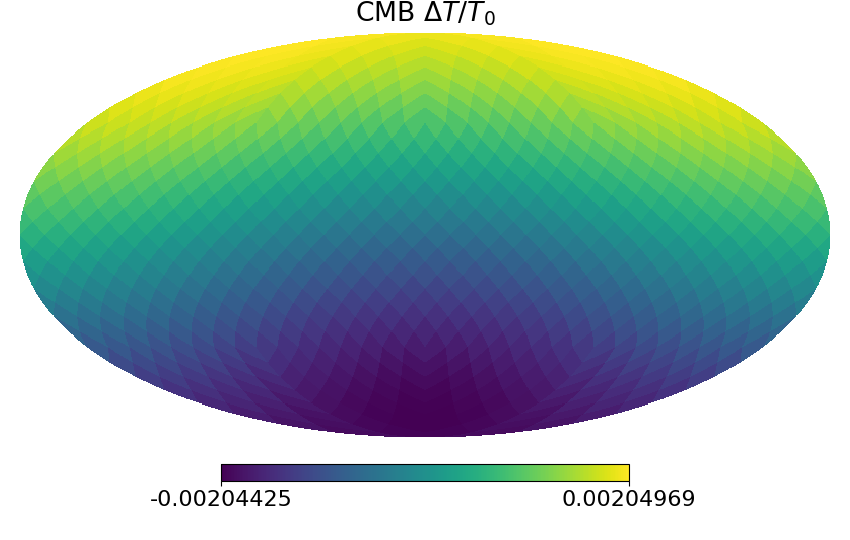
\includegraphics[width=\textwidth]{canonical BNW recomputes/CMB.png}
        \caption{}
    \end{subfigure}
    \begin{subfigure}{0.45\textwidth}
        \centering
        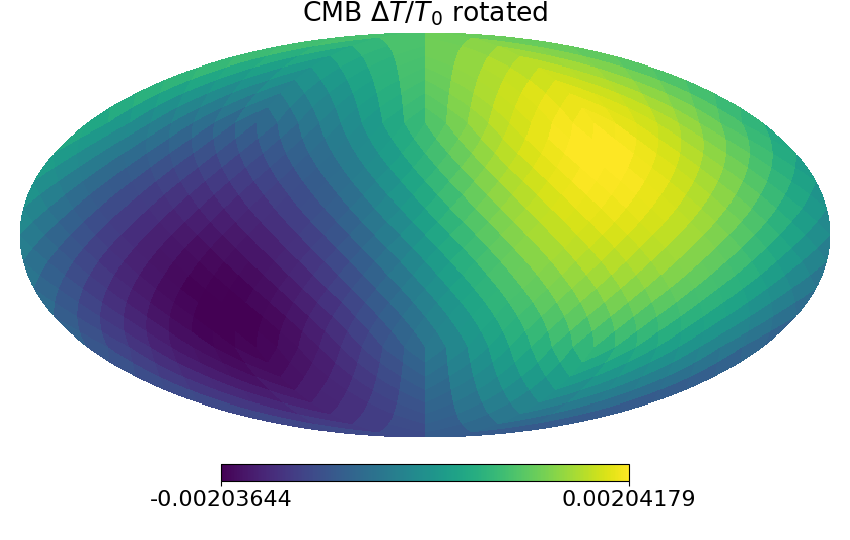
\includegraphics[width=\textwidth]{canonical BNW recomputes/rotated CMB.png}
        \caption{}
    \end{subfigure}
    \caption{Simulated CMB measurement in the canonical BNW model. In (a) it is shown in the frame with $\partial_r$ pointing in the observer's local $z$ direction, i.e., the top of the figure is aligned with $\partial_r$, and the bottom of the figure is aligned with $-\partial_r$. This is the frame we will be using for CMB plots henceforth. In (b) it is rotated to a more familiar frame, where the dipole is aligned with the observed CMB dipole's direction in the galactic coordinate system.}
    \label{fig: canonical BNW CMB}
\end{figure}

\begin{figure}
     \centering
     \begin{subfigure}[b]{105mm}
         \centering
         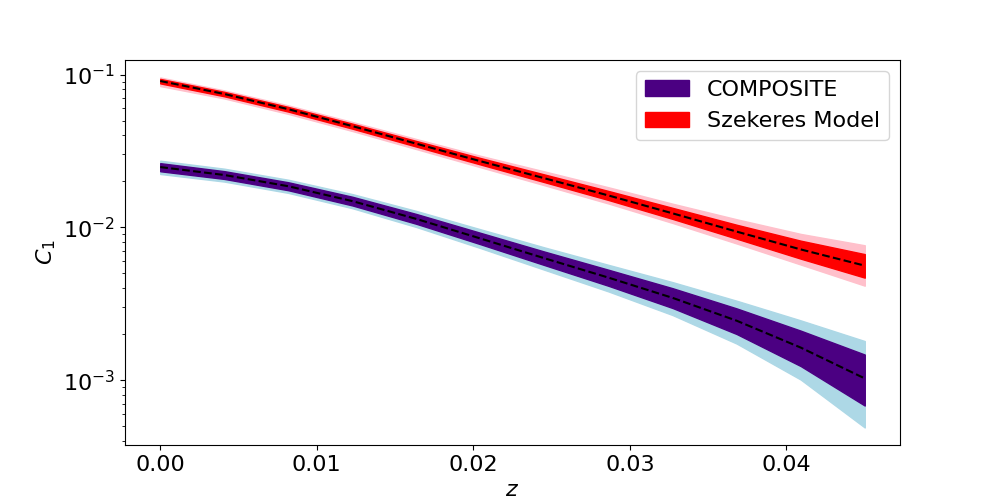
\includegraphics[width=\textwidth]{canonical BNW recomputes/Hub C1.png}
         \caption{}
     \end{subfigure}
     \hfill
     \begin{subfigure}[b]{105mm}
         \centering
         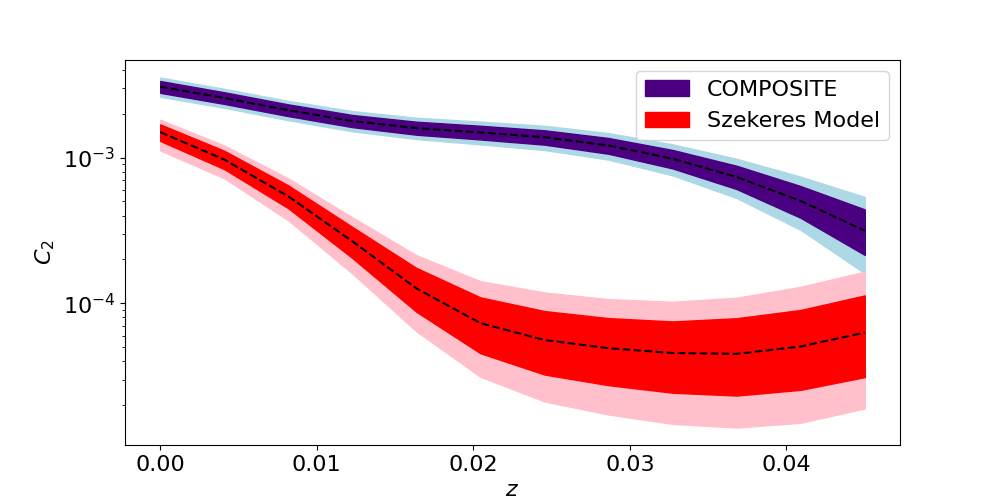
\includegraphics[width=\textwidth]{canonical BNW recomputes/Hub C2.png}
         \caption{}
     \end{subfigure}
      \caption{Simulated Hubble expansion anisotropy in the canonical BNW model. The blue band is the measurement from the COMPOSITE catalogue, and the red band is the values calculated from Szekeres model simulations. Each band show the 65\% and 95\% confidence intervals, and the means are shown with a black dashed line. Figure (a) shows the dipole power $C_1(z)$, and Figure (b) shows the quadrupole power $C_2(z)$.}
      \label{fig: canonical BNW Hubble expansion anisotropy}
\end{figure}

The dipole and quadrupole power of the Hubble expansion anisotropy calculated from the simulated COMPOSITE catalogue are shown in Figure \ref{fig: canonical BNW Hubble expansion anisotropy}. Compared to the power spectrum calculated from the observed COMPOSITE catalogue, we see a higher simulated dipole power than what is observed and a lower simulated quadrupole power than what is observed over all $z$ values. Visually, these are similar to those found by Hills \cite{RN42}, showing consistency of our code.

Unfortunately, the simulated Hubble anisotropy dipole of the canonical BNW does not visually match COMPOSITE as well as is seen in BNW \cite{RN3}. For example, at $z=0$, the simulated dipole is almost an order of magnitude greater than the observed dipole, thus a new set of parameters need to be found.

\section{Exploring Parameter Space with MCMC}\label{section: BNW MCMC}
To explore the parameter space, we use \texttt{emcee}: a Python implementation of Goodman and Weare's Affine Invariant Markov Chain Monte Carlo (MCMC) Ensemble sampler \cite{RN113,RN111}. This method creates a sample of a given probability distribution, and requires significantly less computation time than a grid search. We ran two independent chains for the BNW model, one set only to fit the CMB dipole, and one set to only fit the dipole and quadrupole of the Hubble expansion anisotropy in the COMPOSITE catalogue.

Although the Szekeres solutions are very flexible for exact solutions, they still have very restrictive constraints. Most prominently, the density on each shell must be of a specific form, the dust is irrotational, and one cannot have a collapsing structure that results in a shell crossing during the simulation. Due to these restrictions, it is highly unlikely that a simple Szekeres model will capture all the effects of local structure. It is better to treat them as toy models which provide a reasonable example of the non-linear effects of inhomogeneity. Thus, instead of rigorously deriving a probability distribution of the observable we wish to see, we will provide a heuristic distribution aimed at guiding the Markov Chains towards desirable parameters.

\subsection{MCMC for CMB only}
To direct the Markov Chain towards the correct CMB dipole and quadrupole, we use the following probability density,
\begin{equation} \label{eqn: CMB probability distribution}
    f_{\text{CMB}}(\vec{\alpha}) \propto \exp{\left[-\frac{(\Delta T_{\text{sim}}(\vec{\alpha}) - \Delta T_{\text{obs}})^2}{2\sigma_{\Delta T}^2}\right]} f_{\text{CMB}, \mathcal{D}_2}(\vec{\alpha}),
\end{equation}
where $\vec{\alpha}$ are the model parameters. The first factor is proportional to the probability of observing the simulated CMB temperature dipole given only the uncertainty in determining the observed quantity, where $\Delta T_{\text{sim}}(\vec{\alpha})$ is the simulated CMB temperature dipole amplitude, $\Delta T_{\text{obs}} = 5.66\, \si{mK}$ is the observed CMB temperature dipole amplitude in the Local Group frame, and $\sigma_{\Delta T} = 0.36\, \si{mK}$ is the uncertainty in the observed CMB temperature dipole. The second factor $f_{\text{CMB}, \mathcal{D}_2}$ is proportional to the probability density of observing the quadrupole, chosen heuristically to be
\begin{equation}
    f_{\text{CMB}, \mathcal{D}_2}(\vec{\alpha}) =
    \begin{cases}
        1 & \mathcal{D}_{2, \text{sim}} (\vec{\alpha}) < \mathcal{D}_{2, \text{obs}} \\
        \exp\left[-\frac{(\mathcal{D}_{2, \text{sim}} (\vec{\alpha}) - \mathcal{D}_{2, \text{obs}})^2}{2\sigma_{\mathcal{D}_2}^2}\right] & \text{otherwise}
    \end{cases},
\end{equation}
where $\mathcal{D}_{2, \text{sim}} (\vec{\alpha})$ is the simulated CMB temperature quadrupole, $\mathcal{D}_{2, \text{obs}} = 242.2\: (\mu\text{K})^2$ is the mean observed CMB temperature quadrupole, and $\sigma_{\mathcal{D}_2} = 2\,\mathcal{D}_{2, \text{obs}}$.

\begin{figure}
    \centering
    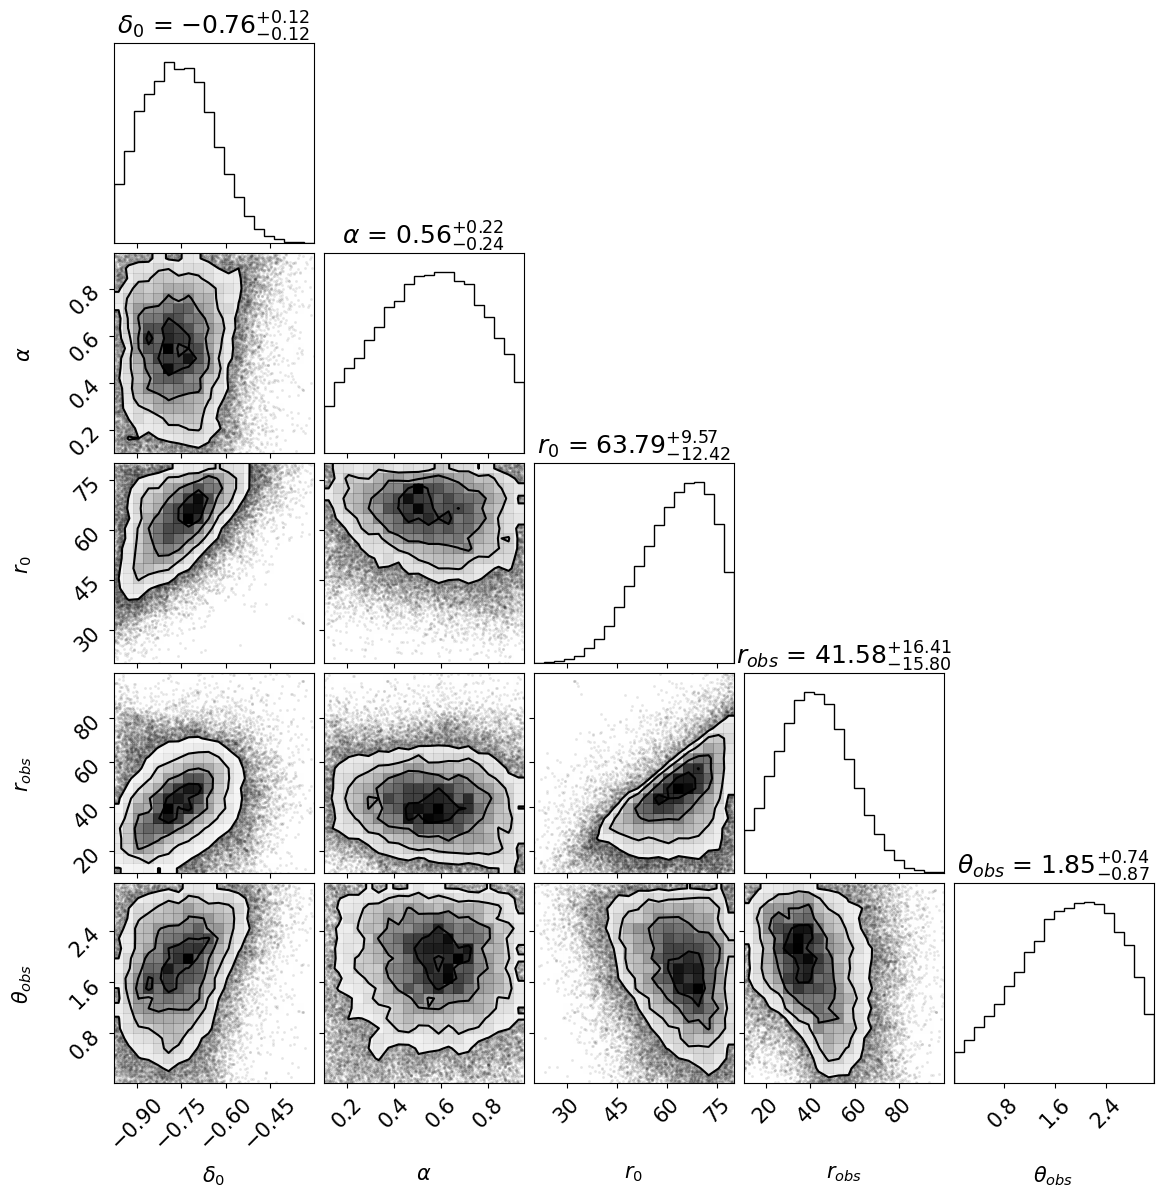
\includegraphics[width=0.9\textwidth]{BNW Model MCMC/cmb only mcmc_no_quad_restriction.png}
    \caption{The one-dimensional and two-dimensional marginal posterior distributions resulting from the MCMC process prescribed to fit the simulated CMB dipole amplitude of the BNW model. Note that the chain used to generate this figure does not attempt to restrict the simulated CMB quadrupole power to a low value.}
    \label{fig: BNW CMB dipole only MCMC corner}
\end{figure}

Figure \ref{fig: BNW CMB dipole only MCMC corner} shows the approximate one-dimensional and two-dimensional marginal posterior distributions over parameter space when fitting the CMB dipole amplitude only (i.e., only using the first term of \eqref{\ref{eqn: CMB probability distribution}}). The two-dimensional marginal probability distributions are given analytically by integrating over all parameters except for two,
\begin{equation}
    k(\alpha_i, \alpha_j) = \int f_{\text{CMB}}(\vec{\alpha}) \diff{\alpha_1} ... \diff{\alpha_{i-1}} \diff{\alpha_{i+1}} ... \diff{\alpha_{j-1}}\diff{\alpha_{j+1}} ... \diff{\alpha_m},
\end{equation}
where $\alpha_i$ are the parameters, and $m$ is the number of parameters. The one dimensional marginal distributions are given similarly, with one integrating over all parameters except one.

From Figure \ref{fig: BNW CMB dipole only MCMC corner} we see that the posterior distribution is well spread -- there is a wide range of parameters where one can find a good fit to the CMB dipole. Notably, the CMB dipole requires a fairly large void, with most of the sample population having $r_0 > 40\, h^{-1}\,$Mpc. There also seems to be a slight preference to larger $\theta_{\text{obs}}$ values, signifying an observer closer to the overdensity; and there is a preference for deeper voids, as seen in the marginal probability distribution of $\delta_0$.

The radial position of the observer $r_\text{obs}$ seems correlated with the size of the void $r_0$ in the sense that $r_\text{obs}$ seems to be restricted to being less than $r_0$. Physically, this is interpreted as the observer being inside or on the edge of the void. There is a similar correlation between $\delta_0$ and $r_0$, where larger voids (larger $r_0$) can have shallower density contrasts (less negative $\delta_0$) and still fit the CMB dipole.

A larger $\alpha$ creates a smaller and sharper overdensity, so if the observer needs to be located in or around the overdensity to observe a consistent CMB dipole, one might expect $\alpha$ to affect the distribution of $\theta_\text{obs}$. However, there is no apparent correlation between $\alpha$ and $\theta_\text{obs}$.


\subsection{MCMC for Hubble Expansion Anisotropy only}\label{sec: BNW Model Fitting COMPOSITE only}
To direct the Markov Chain towards a satisfactory dipole and quadrupole in the Hubble expansion anisotropy, we need to prescribe an appropriate probability distribution function on the angular power spectrum of $H_0 (l,b,z)$. We choose to sample the simulated dipole power $C_{1,\text{sim}} (z_i)$ and quadrupole power $C_{2,\text{sim}} (z_i)$ of $H_0 (l,b,z_i)$ at 12 equally spaced fixed redshifts $z_i$ between $z_1=0$ and $z_{12}=0.045$, and assign a multivariate Gaussian over these 24 variables. The probability density is then proportional to
\begin{equation}\label{eqn: COMPOSITE probability}
    f_\text{COMPOSITE}(\vec{\alpha}) = \exp\left[-\vec{R}^\intercal \Sigma^{-1} \vec{R}\right],
\end{equation}
where $\vec{R}$ is the residual dipole and quadrupole concatenated into a vector
\begin{equation}
    R_i =
    \begin{cases}
        C_{1, \text{sim}} (z_i) - \langle C_{1, \text{obs}} (z_i) \rangle & i \leq 12 \\
        C_{2, \text{sim}} (z_{i-12}) - \langle C_{2, \text{obs}} (z_{i-12}) \rangle & i > 12
    \end{cases},
\end{equation}
and $\Sigma$ is the covariance matrix, calculated from a sample of 10,000 random drawings of observed COMPOSITE catalogue. As $\vec{R}$ has 12 dipole power components and 12 quadrupole power components, the covariance matrix can be split into four minors,
\begin{equation}\label{eqn: COMPOSITE power sigma}
    \Sigma =
    \begin{bmatrix}
        \Sigma_{C_1, C_1} & \Sigma_{C_1, C_2} \\
        \Sigma_{C_2, C_1} & \Sigma_{C_2, C_2}
    \end{bmatrix}.
\end{equation}
The elements of these matrix minors are
\begin{align}
    \begin{split}\label{eqn: matrix minor expressions}
        \left(\Sigma_{C_1, C_1}\right)_{ij} &= \text{cov}\left[C_{1, \text{obs}} (z_i), C_{1, \text{obs}} (z_j)\right],\\
        \left(\Sigma_{C_1, C_2}\right)_{ij} &= \text{cov}\left[C_{1, \text{obs}} (z_i), C_{2, \text{obs}} (z_j)\right],\\
        \left(\Sigma_{C_2, C_1}\right)_{ij} &= \left(\Sigma_{C_1, C_2}\right)_{ji}, \\
        \left(\Sigma_{C_1, C_1}\right)_{ij} &= \text{cov}\left[C_{2, \text{obs}} (z_i), C_{2, \text{obs}} (z_j)\right].
    \end{split}
\end{align}
In the above equations, $C_{\ell, \text{obs}} (z_i)$ is the angular power of $H_0(l,b,z_i)$ calculated from the observed COMPOSITE catalogue, and $\langle C_{\ell, \text{obs}} (z=z_i) \rangle$ is its mean. The simulated power spectrum $C_{\ell, \text{sim}}$ is calculated using the simulated redshifts $z_{Sz}$ and the mean observed luminosity distances in the COMPOSITE catalogue. We do not construct mock catalogues with random distances to reduce the required computation time during the fitting process. The matrix minors of \eqref{\ref{eqn: matrix minor expressions}} can be seen in Figure \ref{fig: COMPOSITE covariance minors}. In this figure, we see correlation between points with similar redshift, particularly at the low redshifts. It is likely that this arises from the Gaussian window used over redshift. There is also a correlation between the dipoles and quadrupoles at the same $z$ value.

\begin{figure}[t]
    \centering
    \begin{subfigure}[b]{0.3\textwidth}
        \centering
        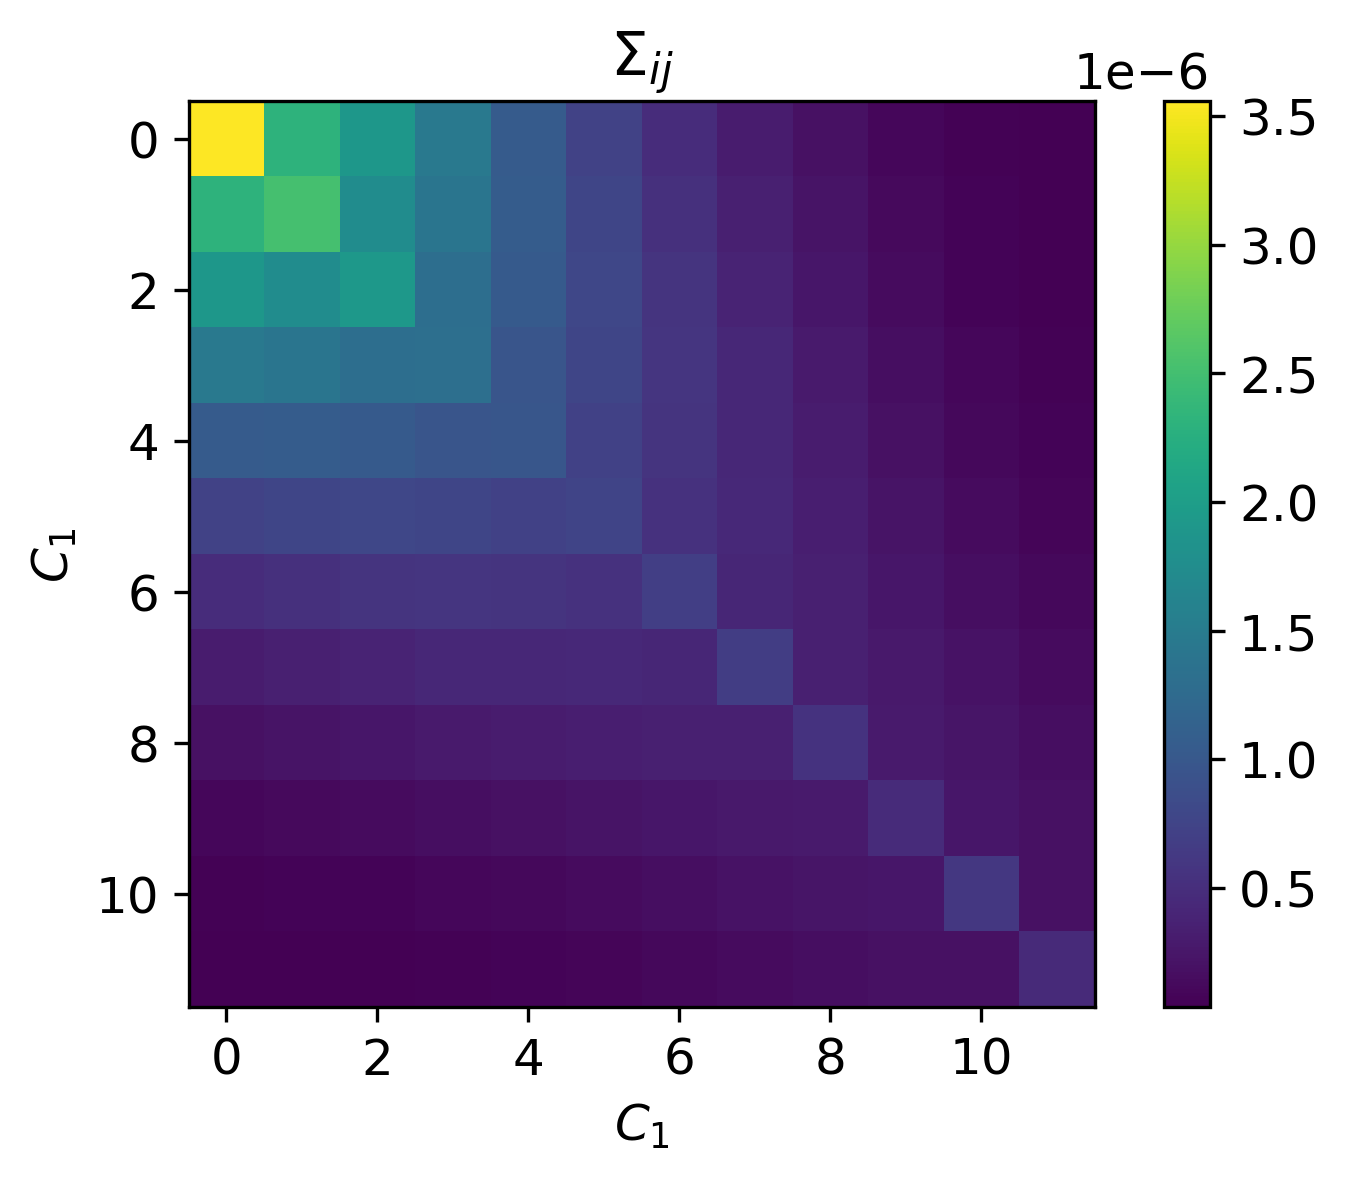
\includegraphics[width=\textwidth]{COMPOSITE cov/dip only cov.png}
        \caption{}
    \end{subfigure}
    \hfill
    \begin{subfigure}[b]{0.3\textwidth}
        \centering
        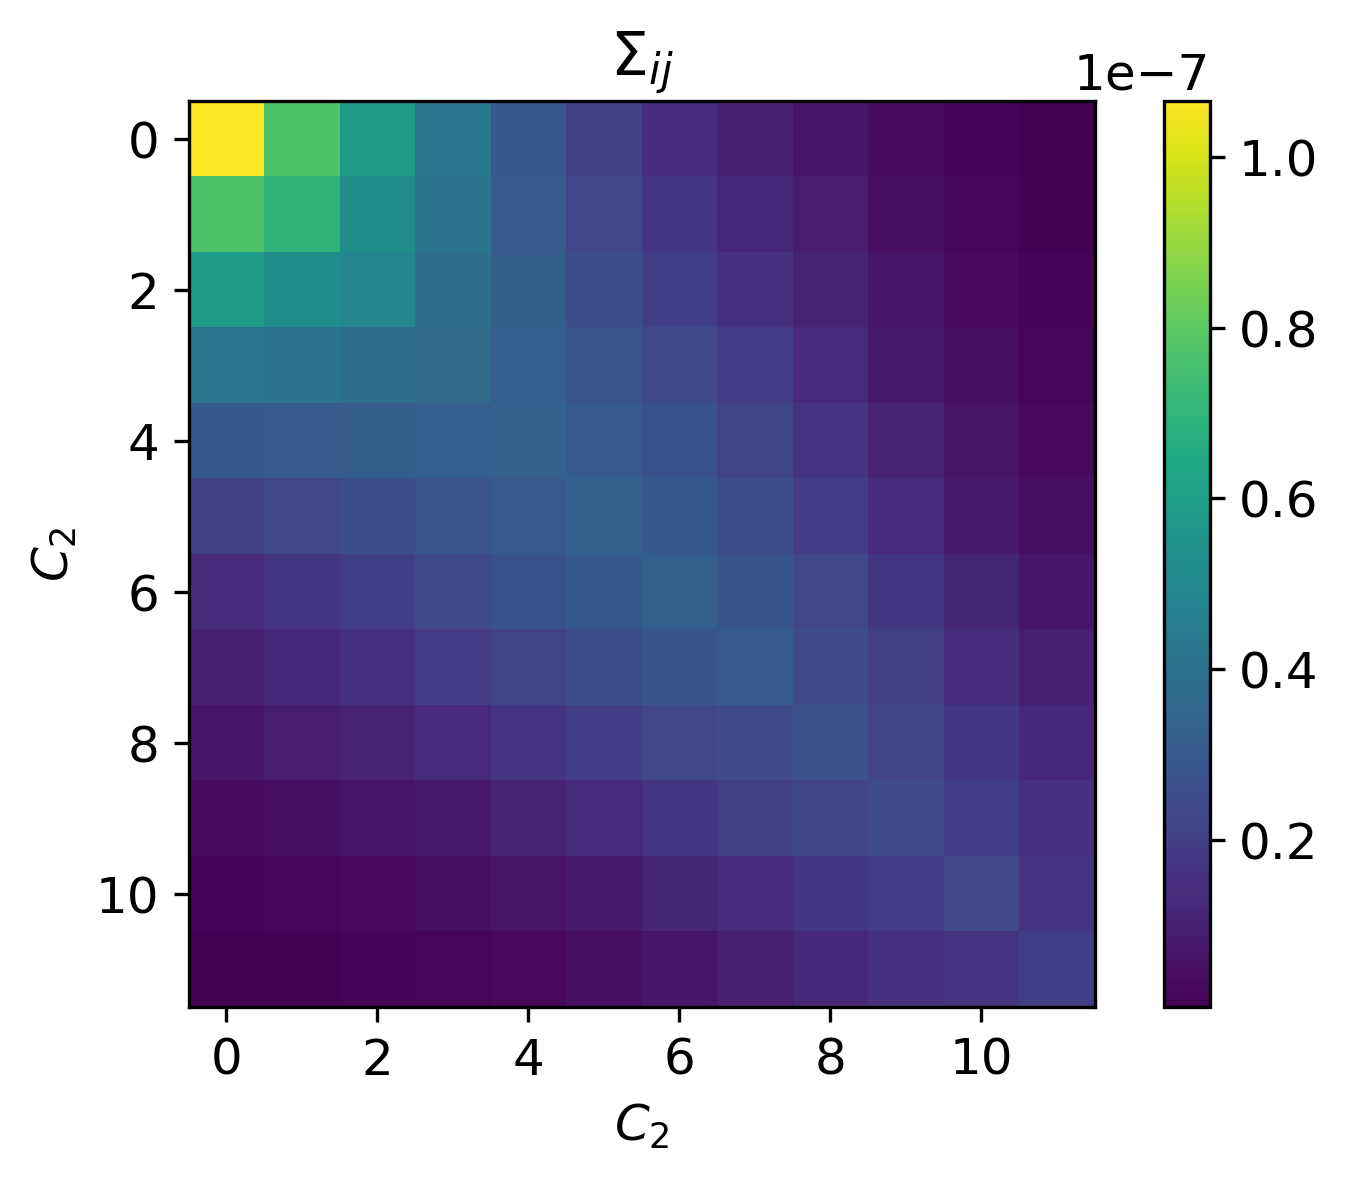
\includegraphics[width=\textwidth]{COMPOSITE cov/quad only cov.png}
        \caption{}
    \end{subfigure}
    \hfill
    \begin{subfigure}[b]{0.3\textwidth}
        \centering
        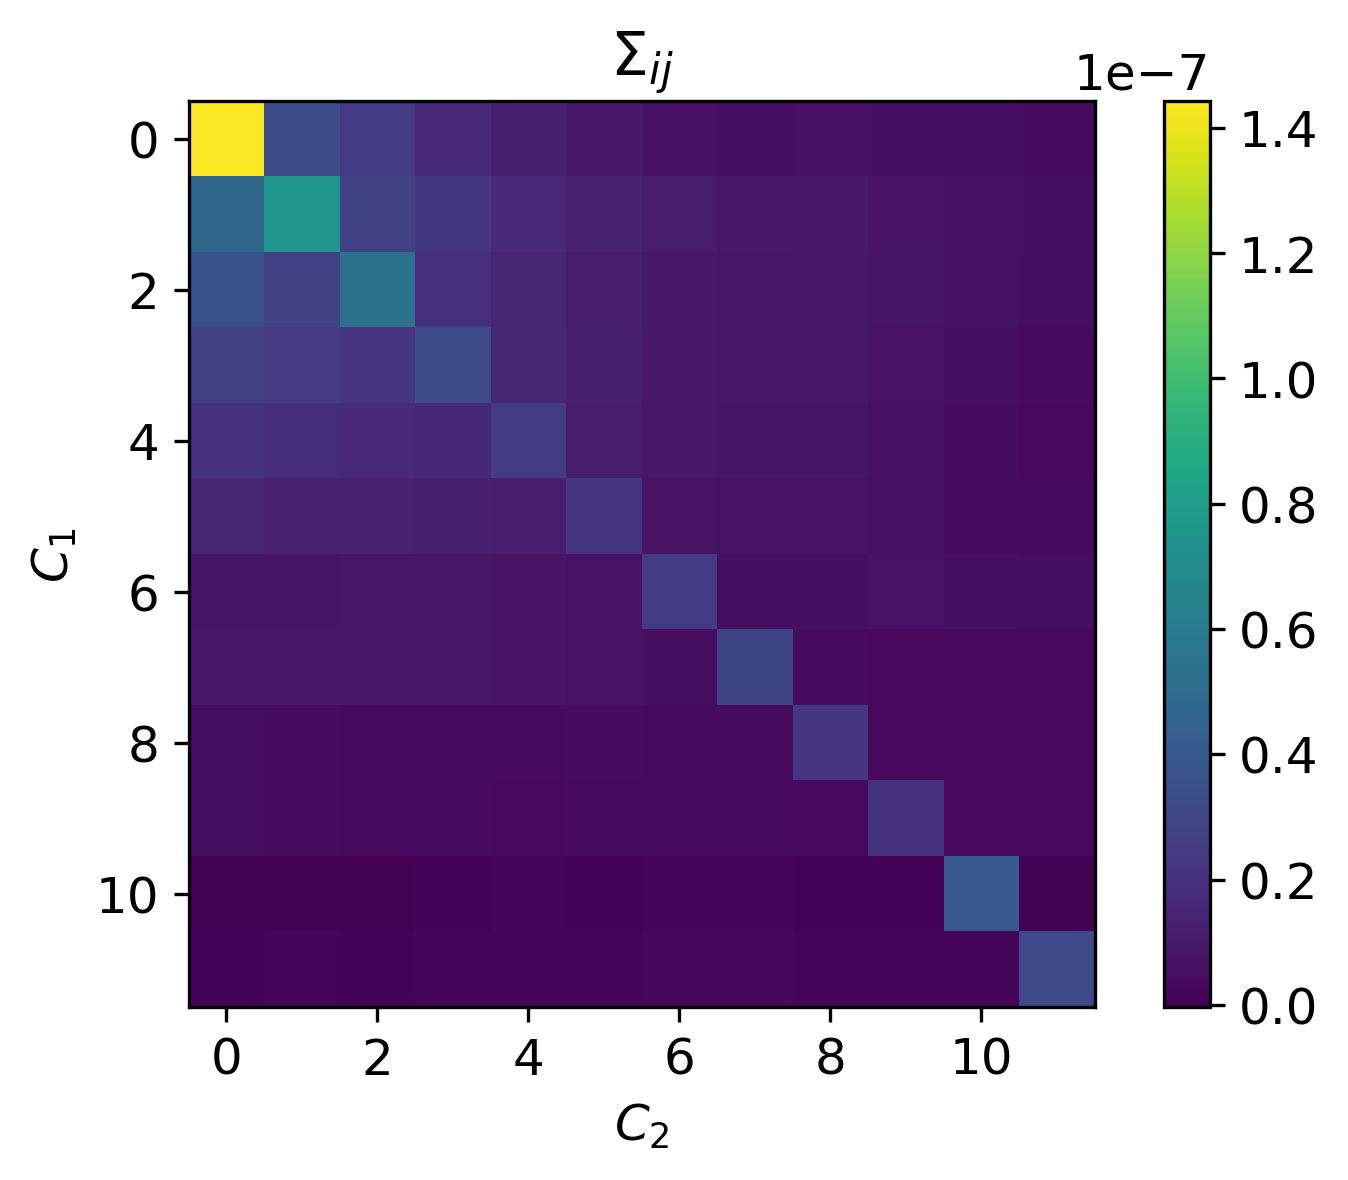
\includegraphics[width=\textwidth]{COMPOSITE cov/dip vs quad cov.png}
        \caption{}
    \end{subfigure}
    \caption{Minors of the covariance matrix $\Sigma$ corresponding to the dipole and quadrupole power of the Hubble expansion anisotropy in the COMPOSITE catalogue. Figure (a) shows the covariance of the dipole power $\Sigma_{C_1, C_1}$, Figure (b) shows the covariance of the quadrupole power $\Sigma_{C_2, C_2}$, and Figure (c) shows the covariance of the dipole power with the quadrupole power $\Sigma_{C_1, C_2}$.}
    \label{fig: COMPOSITE covariance minors}
\end{figure}

Figure \ref{fig: BNW Hubble expansion dip and quad MCMC corner} shows marginal posterior distributions resulting from the chain ran with probability distribution (\ref{eqn: COMPOSITE probability}). Over all parameters, fitting to COMPOSITE gives much tighter restrictions on the parameters and stronger correlations. Notably, the observer is tightly constrained to the edge of the void with $r_\text{obs} \approx r_0$. Some other correlations are particularly apparent, namely between $r_0$ and $\delta_0$, showing that larger voids must be shallower to fit COMPOSITE, but voids with $r_0 \approx 40\, h^{-1}\,$Mpc can have a relatively wide range of $\delta_0$ and still fit to COMPOSITE. The correlation of $r_\text{obs}$ with $\delta_0$ may have arisen due to both of their correlations with $r_0$.

Several of these correlations can be quantified with \textit{Pearson's correlation coefficient}. The correlation coefficient $\rho_{X,Y}$ between two random variables $X$, $Y$ with expected values $\mu_X$, $\mu_Y$, and standard deviations $\sigma_X$, $\sigma_Y$, is defined as
\begin{equation}\label{eqn: pearson correlation coefficient}
    \rho_{X,Y} = \frac{\text{cov}(X,Y)}{\sigma_X \sigma_Y}
    = \frac{\langle (X-\mu_X)(Y-\mu_Y) \rangle}{\sigma_X \sigma_Y},
\end{equation}
where $\langle \rangle$ is the expected value of a random variable. A number close to 1 indicates a strong positive correlation, a number close to -1 indicates a strong negative correlation, and a number close to zero indicates no correlation. For the sample obtained from the MCMC process fitting the BNW model to the COMPOSITE catalogue, the correlation coefficients are shown in Table \ref{tab: BNW correlation coefficients}.

\begin{figure}[!t]
    \centering
    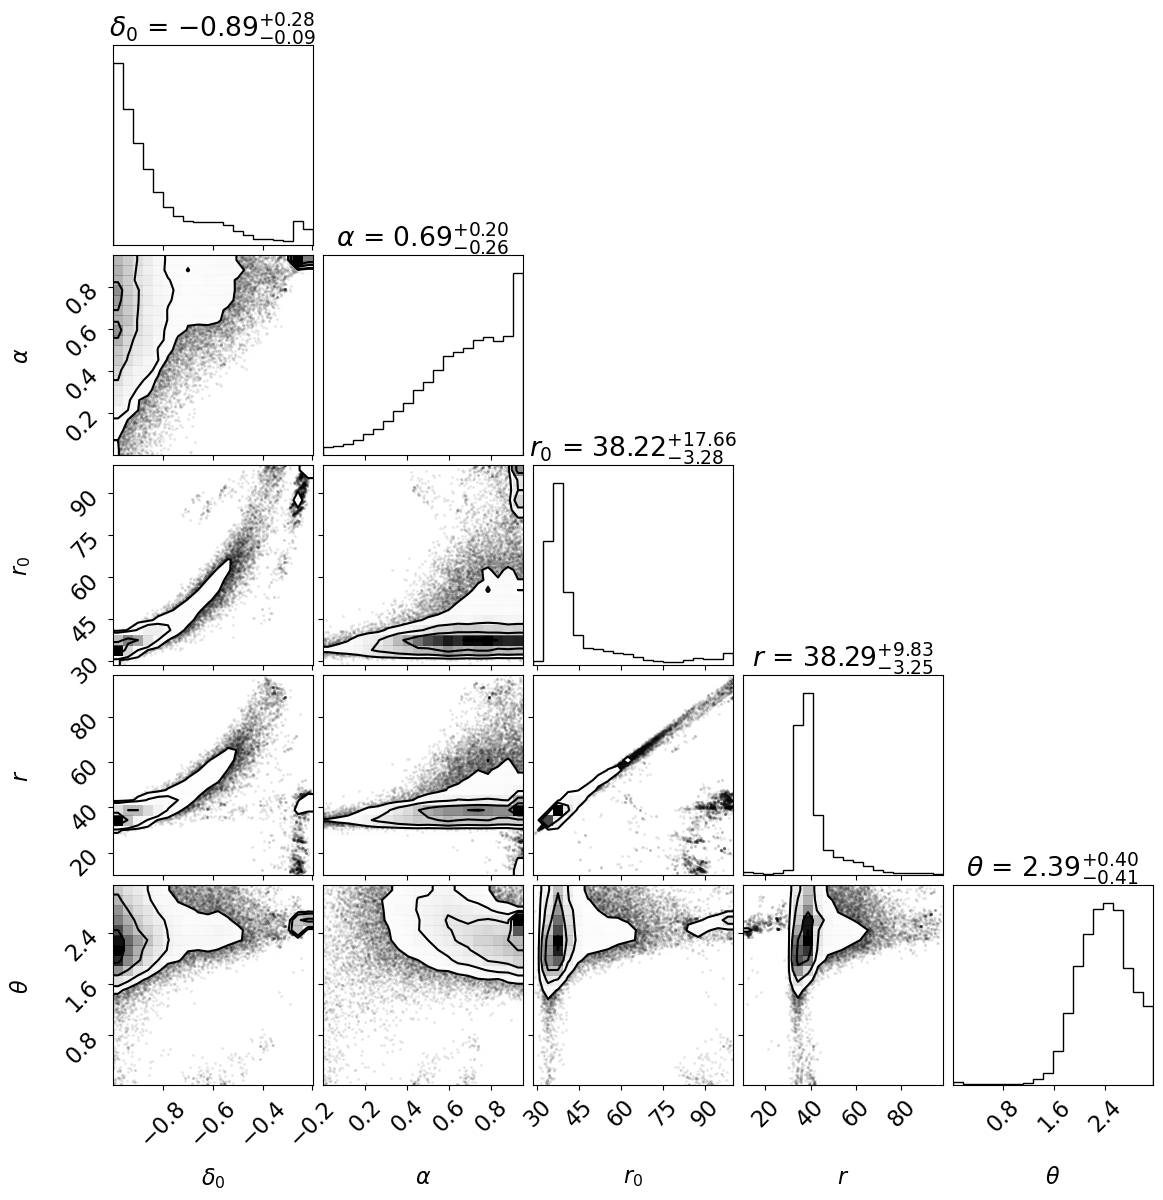
\includegraphics[width=0.9\textwidth]{BNW Model MCMC/composite hubble mcmc dip and quad.png}
    \caption{The one-dimensional and two-dimensional marginal posterior distributions resulting from the MCMC process to fit the BNW model to the Hubble expansion anisotropy dipole and quadrupole seen in the COMPOSITE catalogue. The titles above the plots are the 0.5 quantiles of the distribution of each individual parameter, and their uncertainties are the difference to the 0.16 and 0.84 quantiles. An $x$ quantile is the value of the random variable which has $100x\,\%$ of the sample beneath it. So the $0.5$ quantile is the median.}
    \label{fig: BNW Hubble expansion dip and quad MCMC corner}
\end{figure}

\begin{table}[t]
    \centering
    \begin{tabular}{c|c c c c c}
         & $\delta_0$ & $\alpha$ & $r_0$ & $r_\text{obs}$ & $\theta_\text{obs}$\\
         \hline
        $\delta_0$ & - & - & - & - & - \\
        $\alpha$ & 0.401 & - & - & - & - \\
        $r_0$ & 0.951 & 0.416 & - & - & - \\
        $r_\text{obs}$ & 0.525 & 0.249 & 0.536 & - & - \\
        $\theta_\text{obs}$ & -0.187 & -0.095 & -0.176 & -0.204 & -
    \end{tabular}
    \caption{Pearson correlation coefficients of the MCMC sample obtained from fitting the BNW model to COMPOSITE. A number close to 1 indicates a strong positive correlation, a number close to -1 indicates a strong negative correlation, and a number close to zero indicates no correlation. Note the large correlation coefficients between $r_0$ and $r_\text{obs}$; $r_0$ and $\delta_0$; and $r_\text{obs}$ and $\delta_0$.}
    \label{tab: BNW correlation coefficients}
\end{table}

The model with the greatest value (least negative) of $f_\text{COMPOSITE}$ found in the sample generated by the MCMC process had $\ln(f_\text{COMPOSITE}) = -45$ with the parameters,
\begin{align}
    \begin{split} \label{eqn: best BNW COMPOSITE fit}
        \delta_0 &= -1.0, \\
        \alpha &= 0.95, \\
        r_0 &= 34.6\: h^{-1}\,\text{Mpc}, \\
        r_\text{obs} &= 35.3\: h^{-1}\,\text{Mpc}, \\
        \theta_\text{obs} &= 1.98.
    \end{split}
\end{align}
This can be thought of as the parameter set best fitting to the COMPOSITE catalogue. The simulation results for this model are shown in Figure \ref{fig: CMB and Hubble for BNW best fitting to COMPOSITE}. The simulation results visually match the observed Hubble expansion dipole in COMPOSITE, but not the quadrupole. As this is the best fit to COMPOSITE, this shows that the BNW model cannot simultaneously fit the dipole and quadrupole of the observed Hubble flow. The dipole of the simulated CMB for this parameter set is $\Delta T = 2.96\, \si{mK}$, only 51\% of the observed value. The CMB quadrupole is suitably low at $\mathcal{D}_2 = 44.5\, (\mu \si{K})^2$, only 18\% of the observed quadrupole power. We do not expect a good CMB fit, as this parameter set was obtained from only fitting to COMPOSITE.

The density contrast for this model is shown in Figure \ref{fig: BNW model best COMPOSITE fit density contrast}. Compared to the canonical BNW model (which has density contrast seen in Figure \ref{fig: BNW params density contrast}), the overdensity is smaller and has a much higher peak density contrast due to the larger value of $\alpha$, and the void has a lower density contrast in its centre and has a smaller radius.

\begin{figure}[t]
    \centering
    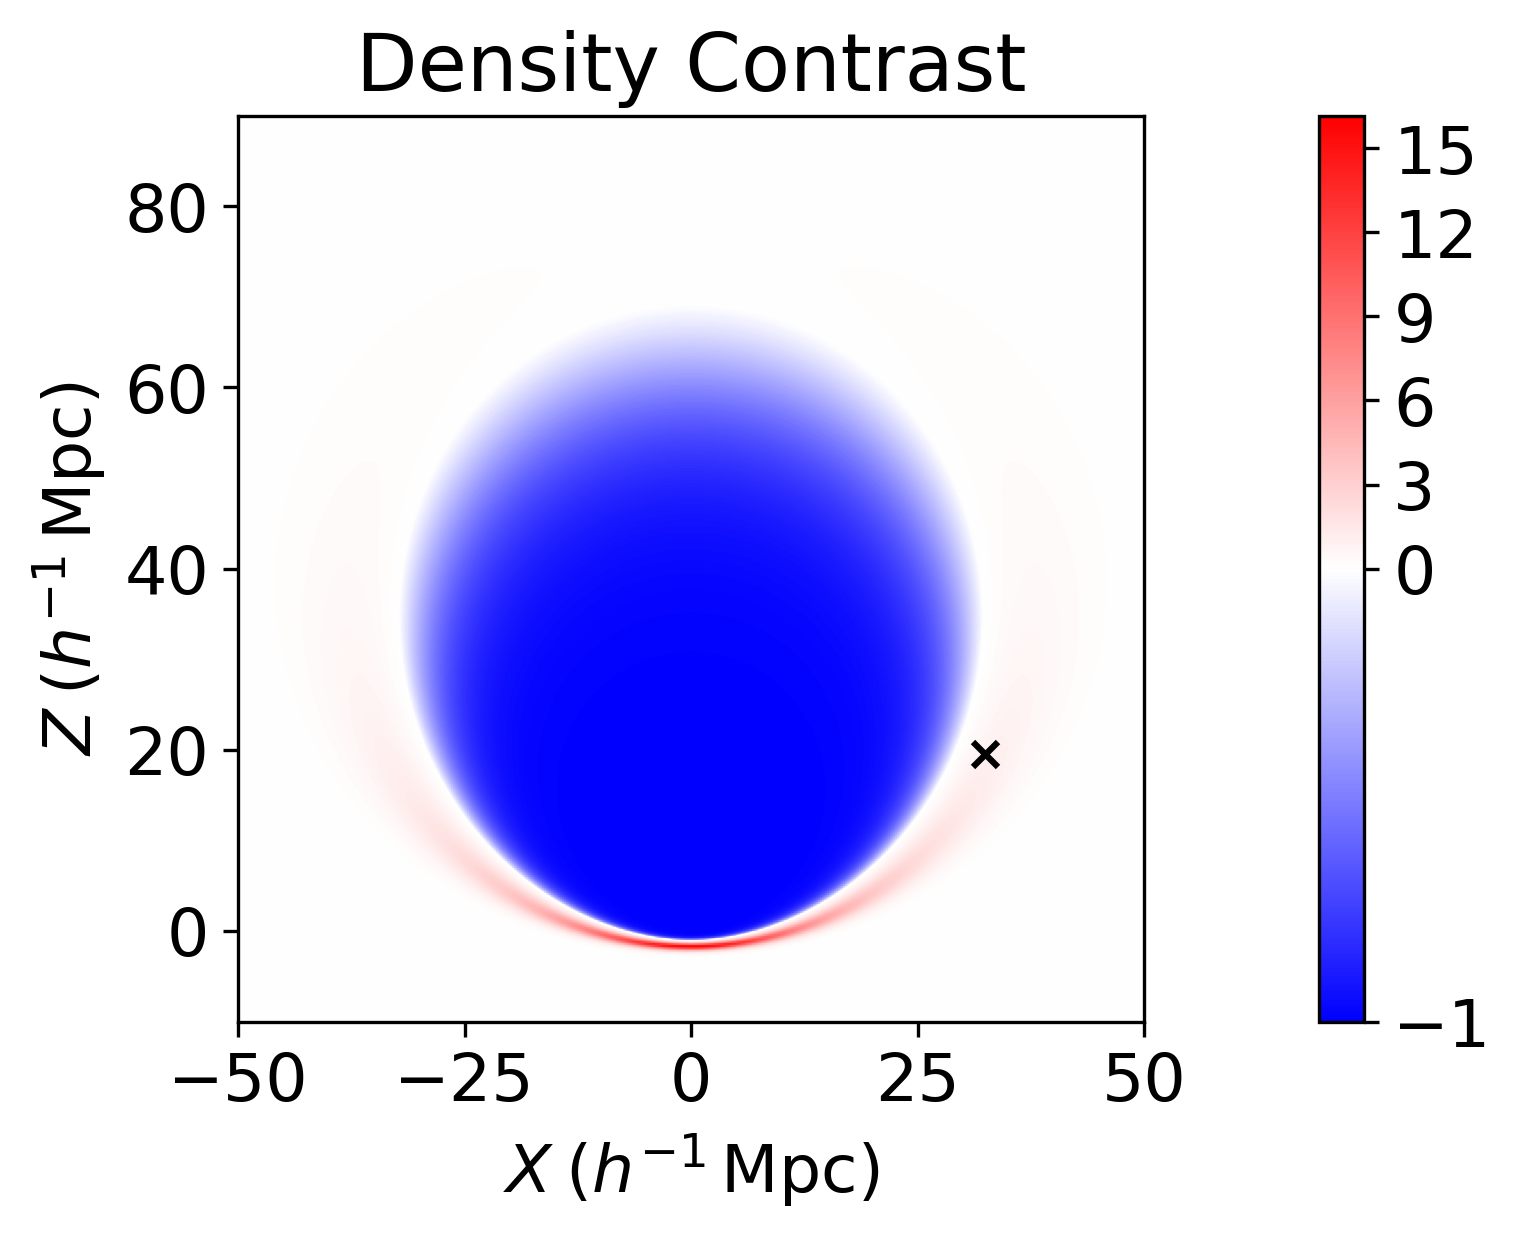
\includegraphics[width=105mm]{BNW Model MCMC/best comp fit/best composite only fit density contrast.png}
    \caption{The density contrast of the BNW model found with the largest value of $f_\text{COMPOSITE}$, i.e., the BNW model which fits the COMPOSITE catalogue the best. The parameters of this model are seen in \eqref{\ref{eqn: best BNW COMPOSITE fit}}. The black cross shows the position of the observer.}
    \label{fig: BNW model best COMPOSITE fit density contrast}
\end{figure}

\begin{figure}[ht]
    \centering
    \begin{subfigure}[b]{105mm}
        \centering
        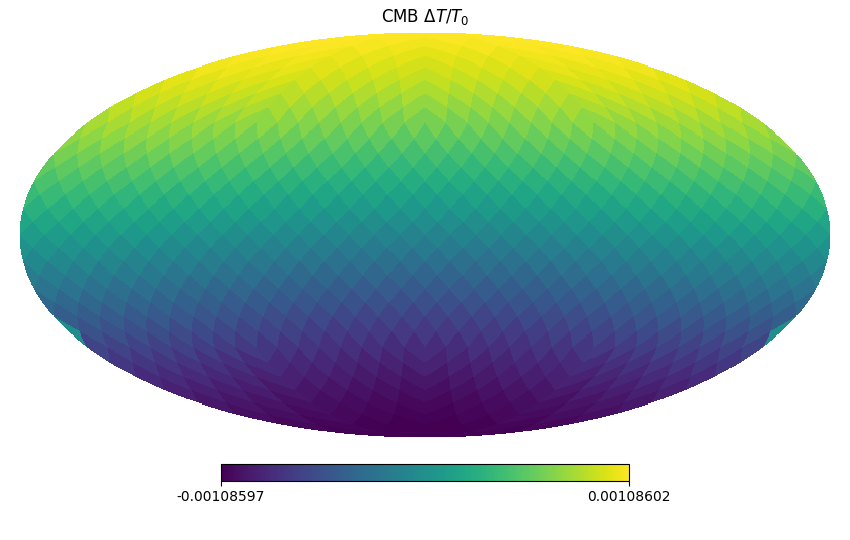
\includegraphics[width=\textwidth]{BNW Model MCMC/best comp fit/CMB.png}
        \caption{}
    \end{subfigure}
    \\
    \begin{subfigure}[b]{105mm}
        \centering
        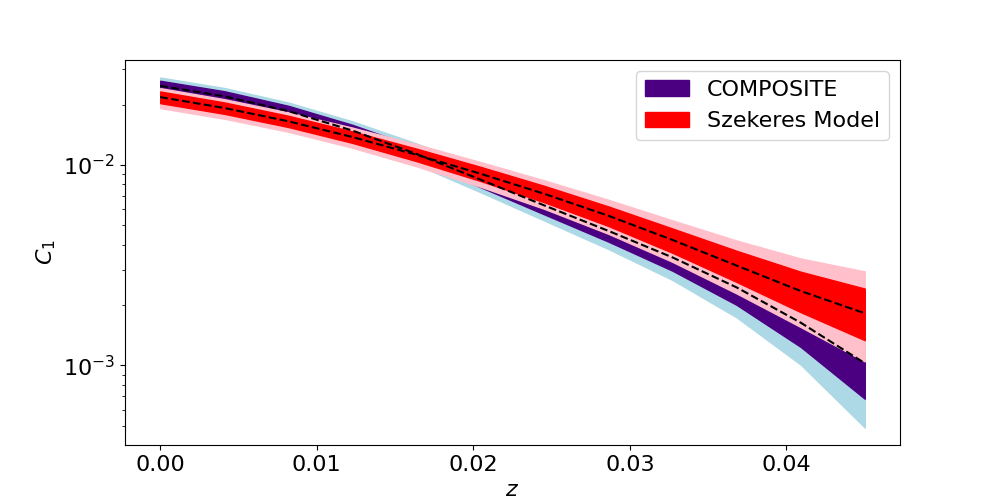
\includegraphics[width=\textwidth]{BNW Model MCMC/best comp fit/Hub C1.png}
        \caption{}
    \end{subfigure}
    \hfill
    \begin{subfigure}[b]{105mm}
        \centering
        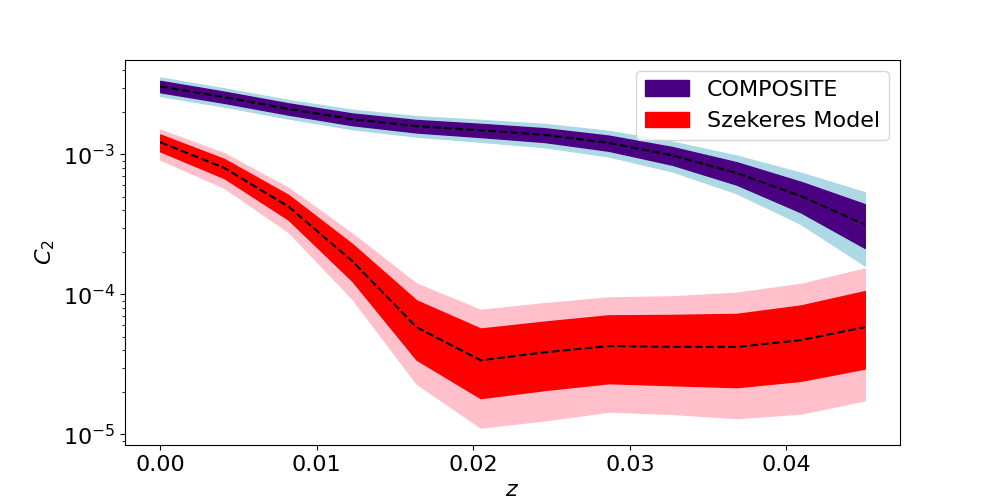
\includegraphics[width=\textwidth]{BNW Model MCMC/best comp fit/Hub C2.png}
        \caption{}
    \end{subfigure}
    \caption{These plots show the simulated observables and compare the simulated COMPOSITE Hubble expansion anisotropy to the observed value. The observables plotted are, (a): the simulated CMB $\Delta T / T_0$, (b): the Hubble expansion anisotropy dipole, and (c): the Hubble expansion anisotropy quadrupole. The simulated quantities are from the BNW model with the largest value of $f_\text{COMPOSITE}$, i.e., the parameter set in (\ref{eqn: best BNW COMPOSITE fit}). The simulated CMB in this model has a dipole of $\Delta T = 2.96\, \si{mK}$ (51\% of the observed value, $7.8\sigma$) and a quadrupole of $\mathcal{D}_2 = 44.5\, (\mu \si{K})^2$ (18\% of the observed power). The CMB in this figure is shown in the frame with the poles pointing in the radial direction, i.e., $\theta=0$ is aligned with $\partial_r$.}
    \label{fig: CMB and Hubble for BNW best fitting to COMPOSITE}
\end{figure}

As an example of a `typical' parameter set fitting to COMPOSITE, we also show 0.5 quantile fit, i.e., the median value of each parameter. These median parameter values are given in the titles of Figure \ref{fig: BNW Hubble expansion dip and quad MCMC corner}. This parameter set has $\ln(f_\text{COMPOSITE}) \approx -48$, not much lower than the best fit found. The density contrast is shown in Figure \ref{fig: BNW model 0.5 quantile density contrast}, and the observables are shown in Figure \ref{fig: BNW COMP MCMC 0.5 quantile observables}. This parameter set has a simulated CMB dipole amplitude of $3.17\,~\si{mK}$ (55\% of the observed value), and a CMB quadrupole power of $2.60\,~(\mu \si{K})^2$ (1\% of the observed power).

\begin{figure}
    \centering
    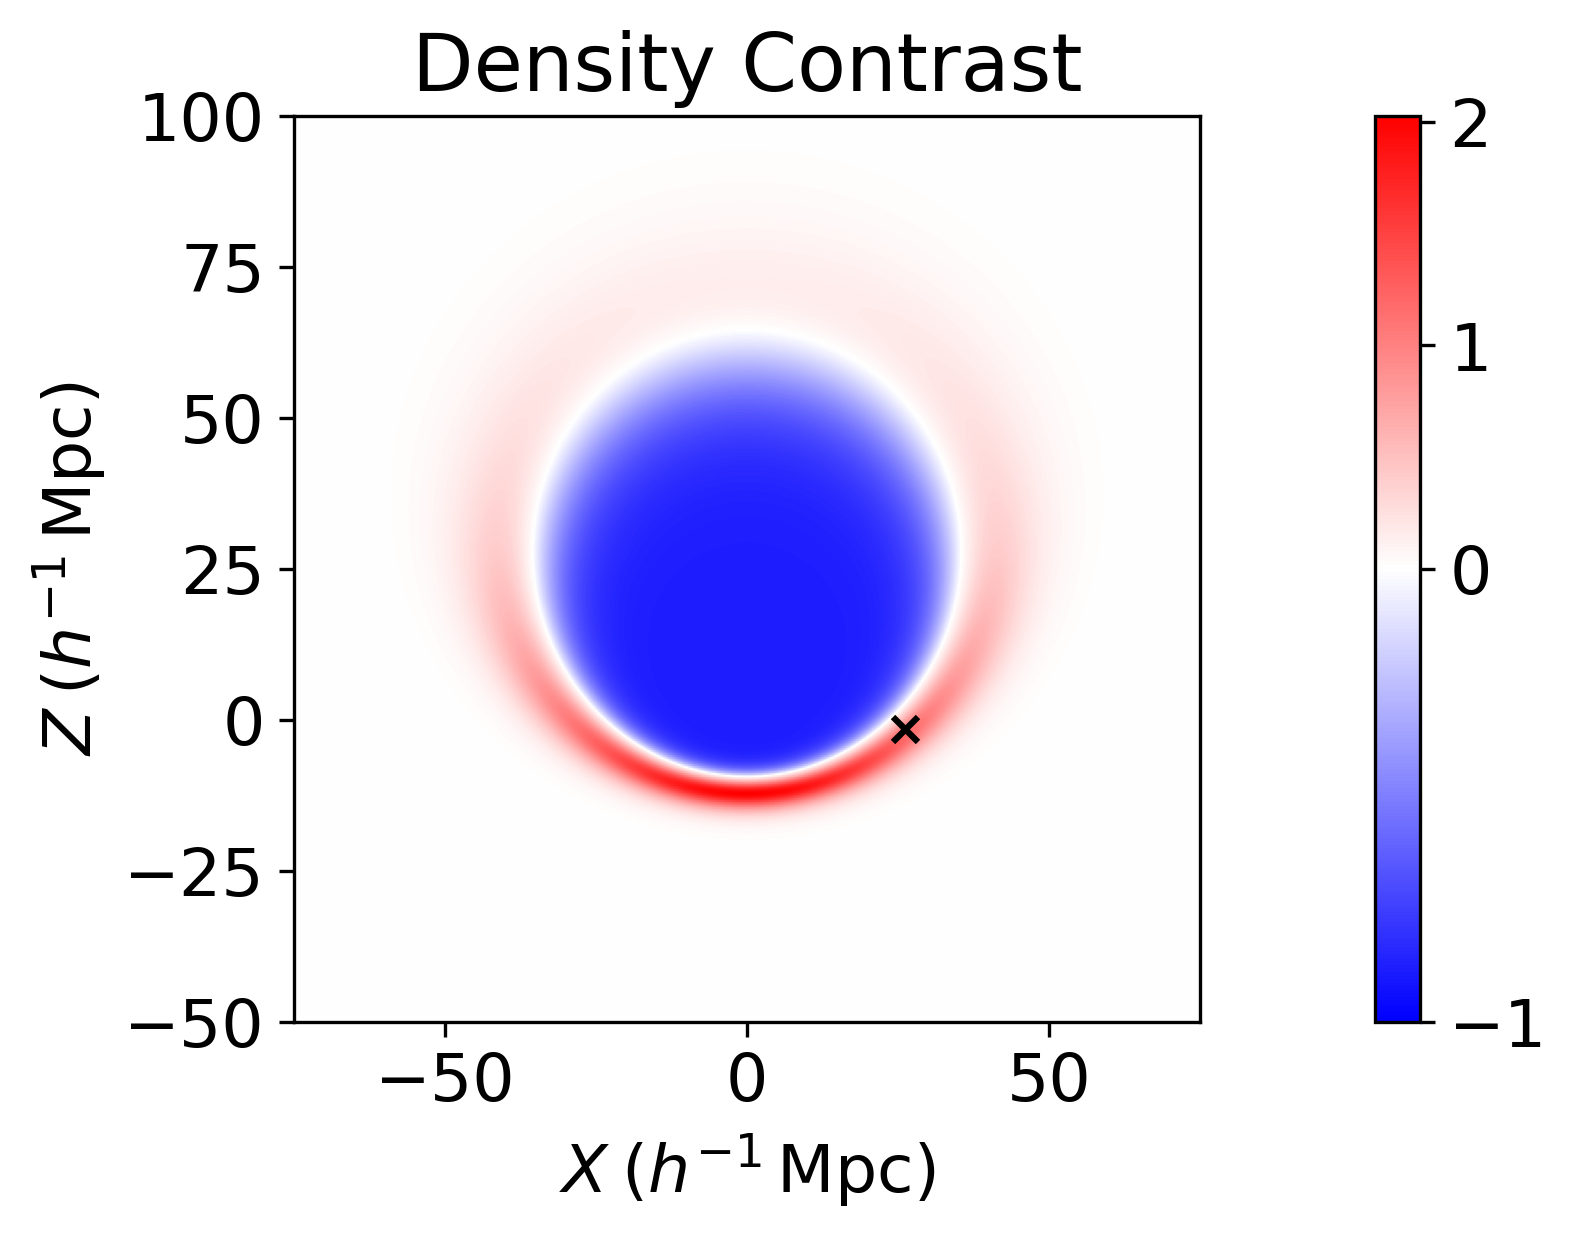
\includegraphics[width=105mm]{BNW Model MCMC/0.5 Quantile/density contrast.png}
    \caption{The density contrast of the 0.5 quantile BNW model, i.e., the median parameter values from the sample obtained from the MCMC process fitting the BNW model to the COMPOSITE catalogue. The cross marks the position of the observer.}
    \label{fig: BNW model 0.5 quantile density contrast}
\end{figure}

\begin{figure}
    \centering
    \begin{subfigure}[b]{105mm}
        \centering
        \includegraphics[width=\textwidth]{BNW Model MCMC/0.5 Quantile/CMB.png}
        \caption{}
    \end{subfigure}
    \\
    \begin{subfigure}[b]{105mm}
        \centering
        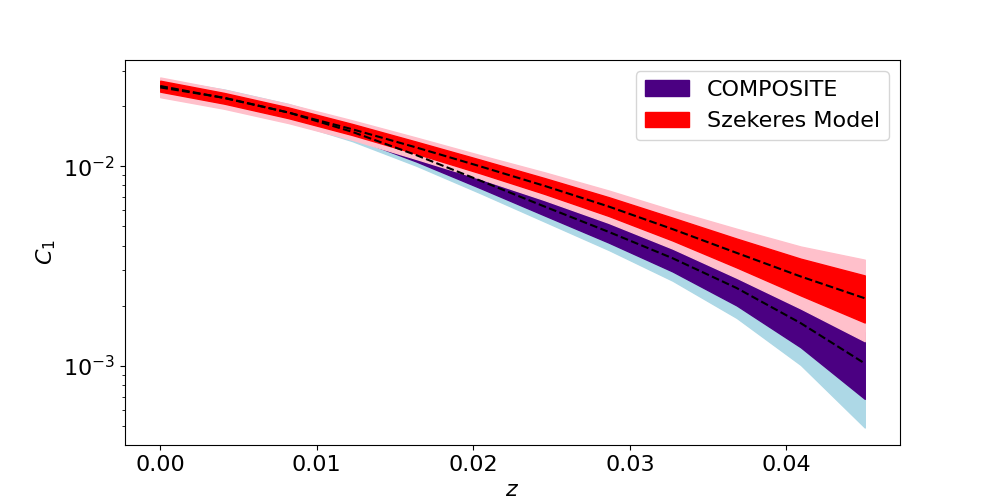
\includegraphics[width=\textwidth]{BNW Model MCMC/0.5 Quantile/Hub C1.png}
        \caption{}
    \end{subfigure}
    \hfill
    \begin{subfigure}[b]{105mm}
        \centering
        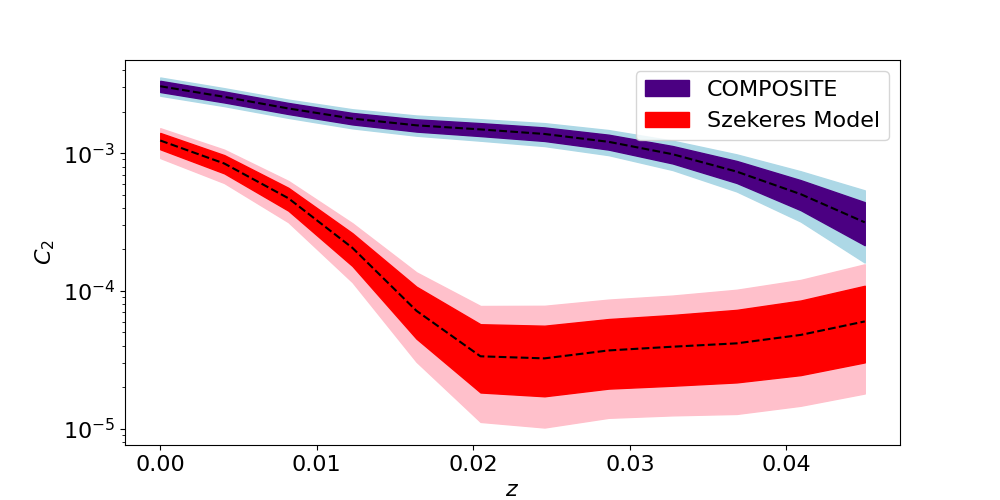
\includegraphics[width=\textwidth]{BNW Model MCMC/0.5 Quantile/Hub C2.png}
        \caption{}
    \end{subfigure}
    \caption{These plots show the simulated observables and compare the simulated COMPOSITE Hubble expansion anisotropy to the observed value. The observables plotted are, (a): the simulated CMB $\Delta T / T_0$, (b): the Hubble expansion anisotropy dipole, and (c): the Hubble expansion anisotropy quadrupole. The simulated quantities are from the median parameter values yielded from the MCMC process. The CMB has a dipole of $\Delta T = 3.17\, \si{mK}$ (55\% of the observed value, $7.2\sigma$) and a quadrupole of $\mathcal{D}_2 = 2.60\, (\mu \si{K})^2$ (1\% of the observed value). The CMB in this figure is shown in the frame with the poles pointing in the radial direction, i.e., $\theta=0$ is aligned with $\partial_r$.}
    \label{fig: BNW COMP MCMC 0.5 quantile observables}
\end{figure}

\section{CMB and COMPOSITE}\label{section: BNW model fitting CMB and COMPOSITE}
In this section, we compare and contrast the results obtained from attempting to fit to the CMB dipole and COMPOSITE individually, aiming to find a geometry that fits both datasets simultaneously.

Figure \ref{fig: marginal r_0 and r_obs comparison} compares the two-dimensional marginal distributions over $r_0$ and $r_\text{obs}$ obtained when fitting the BNW model to the CMB dipole amplitude (red), and the COMPOSITE catalogue (blue). One can see that the majority of the peak obtained when fitting to COMPOSITE is outside the region where a CMB dipole fit can be found. There is some overlap in $r \gtrsim 50\, h^{-1}\,$Mpc, but the probability density when fitting to COMPOSITE is somewhat low here. Therefore, in this region one may be able to find a small volume of parameter space where both the parameters fit to both CMB and COMPOSITE, or there may be a larger volume of mediocre fits to both.

\begin{figure}[h]
    \centering
    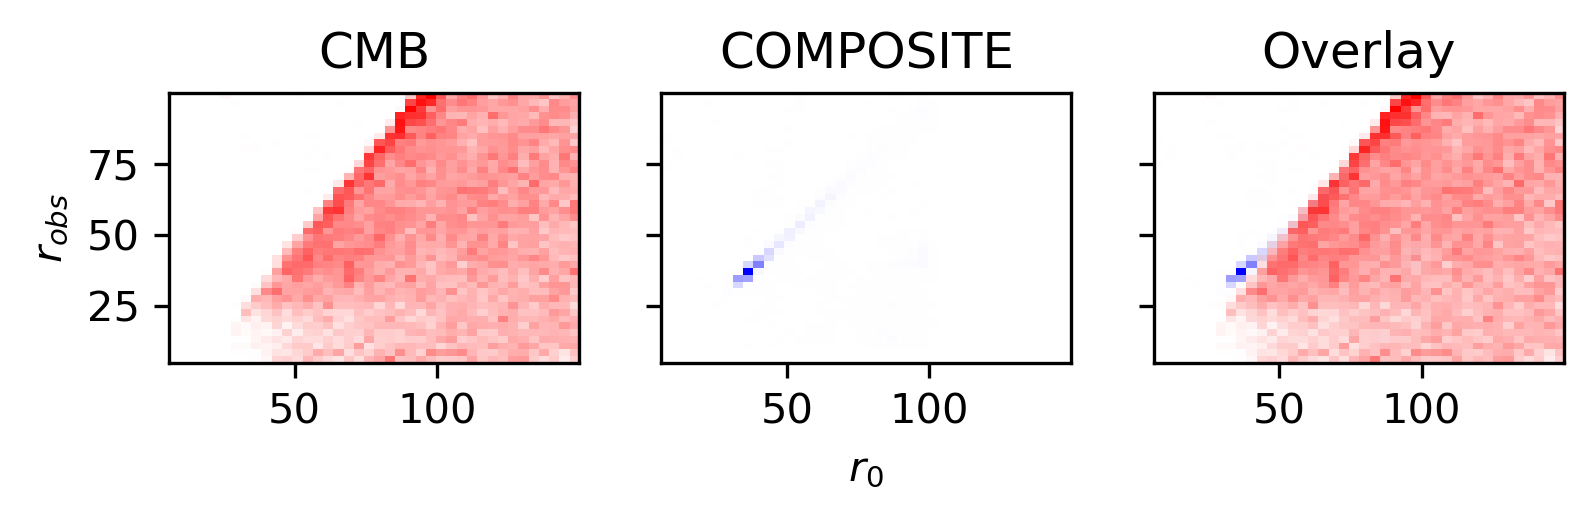
\includegraphics[width=0.9\textwidth]{BNW Model MCMC/Comparisons/CMB vs COMPOSITE r0 vs robs.png}
    \caption{Marginal probability distribution over $r_0$ and $r_\text{obs}$ resulting from fitting to CMB dipole (left) and COMPOSITE (middle). The right figure shows the two overlaid on each other for comparison, where red regions are from fitting to the CMB dipole, and blue regions are from fitting to COMPOSITE.}
    \label{fig: marginal r_0 and r_obs comparison}
\end{figure}

There are a number of geometries one can find (specified by $\delta_0$, $\alpha$, and $r_0$) where an observer in one location fits the CMB dipole, and an observer in a different location fits the COMPOSITE Hubble expansion dipole. For example, the geometry with parameters
\begin{align}
    \begin{split} \label{eqn: BNW special geometry}
        \delta_0 &= -0.63, \\
        \alpha &= 0.83, \\
        r_0 &= 56.7\: h^{-1}\, \text{Mpc}.
    \end{split}
\end{align}
When simulating an observer at $r_\text{obs}=49.9\, h^{-1}\, \text{Mpc}$ and $\theta_\text{obs} = 2.95$, we get a CMB dipole of $5.03\, \si{mK}$ (87\% of the observed value) which is just within $2\sigma$ of the observed CMB dipole, the simulated CMB quadrupole power for this observer is $16.0\, (\mu\si{K})^2$ which is well below the observed value (7\% of the observed power). However, the simulated dipole power of the Hubble expansion anisotropy is too large at all redshifts. An alternative observer at $r_\text{obs}=56.6\, h^{-1}\, \text{Mpc}$ and $\theta_\text{obs} = 2.58$ observes a much lower CMB dipole of $3.36\, \si{mK}$ (58\% of the observed value), and observes a simulated CMB quadrupole power of $2.68\, (\mu\si{K})^2$ (1\% of the observed value), but has a much better fitting Hubble anisotropy. The results of these simulations are seen in Figure \ref{fig: special geometry different observers}, and the density contrast and position of the two observers can be seen in Figure \ref{fig: special geometry density contrast}.

There are other geometries like this, where one observer only matches the CMB and another observer only matches the COMPOSITE catalogue. These geometries all have voids with a radius in the range $54\, h^{-1}\, \text{Mpc} < r_0 < 57\, h^{-1}\, \text{Mpc}$. However, from the samples generated by the two MCMC processes we were unable to find any with observers much closer than those seen in Figure \ref{fig: special geometry density contrast}, suggesting that a satisfactory fit to both the CMB dipole and COMPOSITE Hubble expansion anisotropy cannot be found.

\begin{figure}[t]
    \centering
    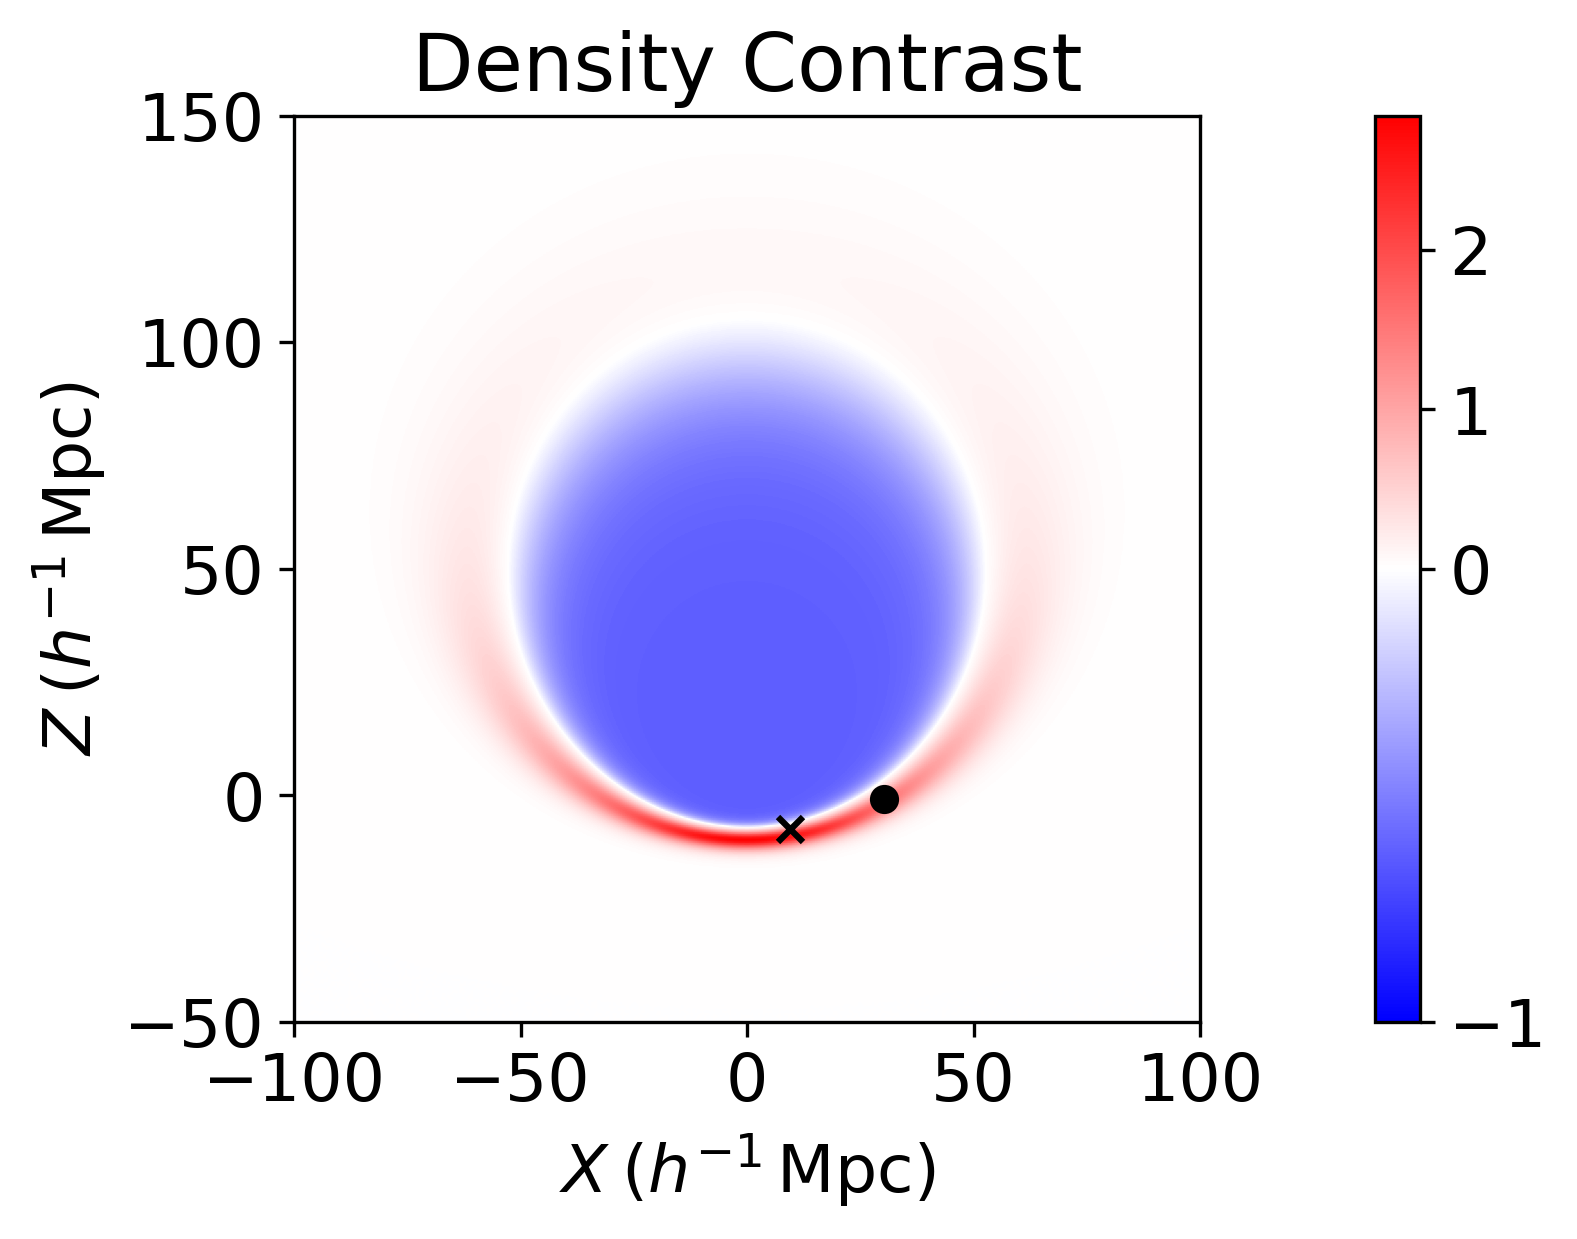
\includegraphics[width=105mm]{Figures/BNW Model MCMC/Special Geometry One/density contrast.png}
    \caption{The density contrast for the geometry specified by \eqref{\ref{eqn: BNW special geometry}}. The cross marker shows the position of the observer which observed a simulated CMB dipole just within $2\sigma$ of our observed value, but has a dipole power in the COMPOSITE Hubble expansion anisotropy which is too large. The solid circle marker shows the position of the observer which visually fits the dipole power in the COMPOSITE Hubble expansion anisotropy, but has a CMB dipole which is too small.}
    \label{fig: special geometry density contrast}
\end{figure}

\begin{figure}[t]
    \centering
    %% CMB
    \begin{subfigure}[b]{0.45\textwidth}
        \centering
        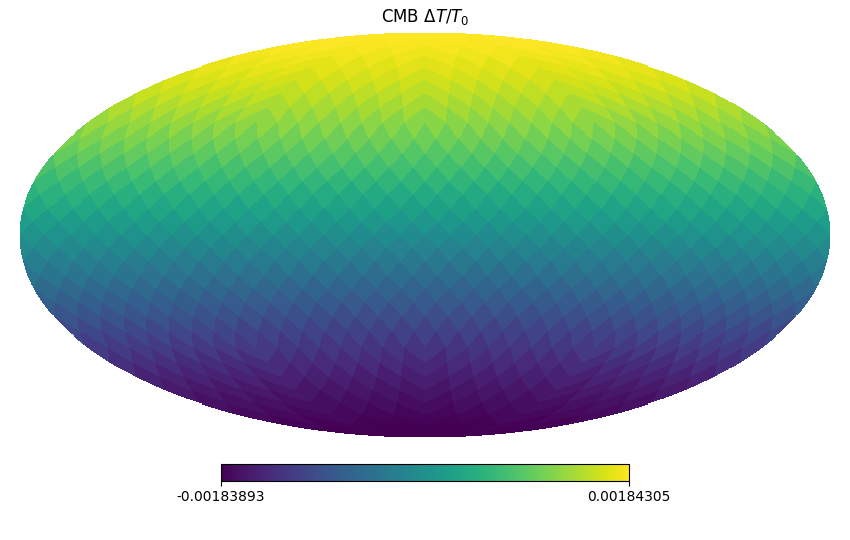
\includegraphics[width=\textwidth]{BNW Model MCMC/Special Geometry One/CMB/CMB.png}
        \caption{}
    \end{subfigure}
    \begin{subfigure}[b]{0.45\textwidth}
        \centering
        \includegraphics[width=\textwidth]{BNW Model MCMC/Special Geometry One/COMPOSITE/CMB.png}
        \caption{}
    \end{subfigure}
    %% Hub C1
    \begin{subfigure}[b]{0.45\textwidth}
        \centering
        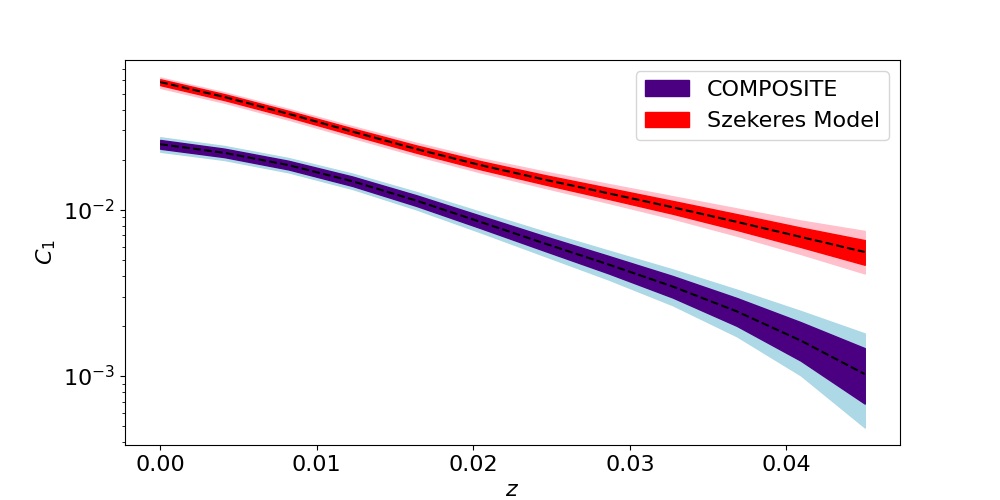
\includegraphics[width=\textwidth]{BNW Model MCMC/Special Geometry One/CMB/Hub C1.png}
        \caption{}
    \end{subfigure}
    \begin{subfigure}[b]{0.45\textwidth}
        \centering
        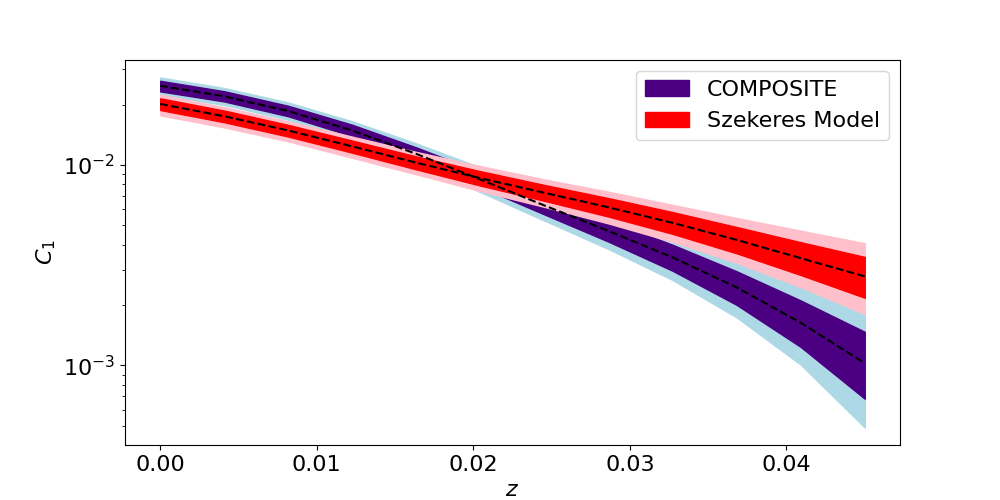
\includegraphics[width=\textwidth]{BNW Model MCMC/Special Geometry One/COMPOSITE/Hub C1.png}
        \caption{}
    \end{subfigure}
    %% Hub C2
    \begin{subfigure}[b]{0.45\textwidth}
        \centering
        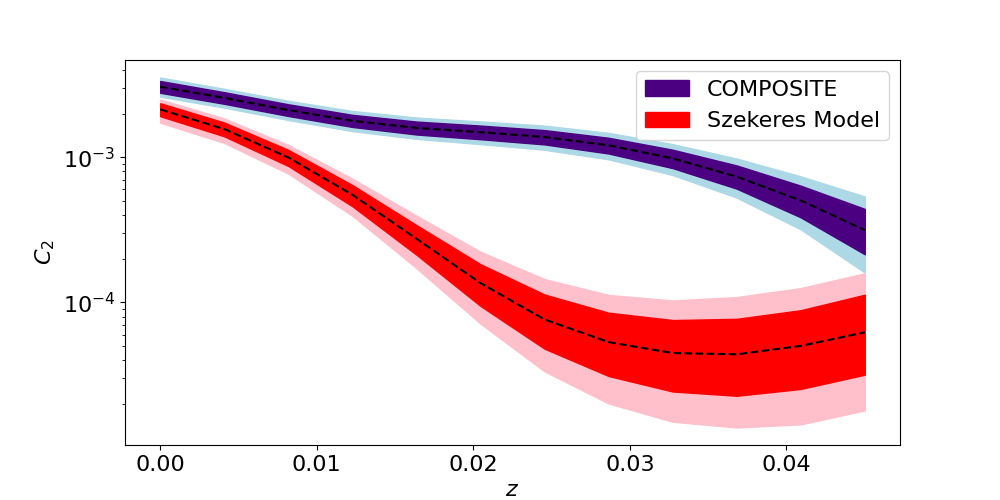
\includegraphics[width=\textwidth]{BNW Model MCMC/Special Geometry One/CMB/Hub C2.png}
        \caption{}
    \end{subfigure}
    \begin{subfigure}[b]{0.45\textwidth}
        \centering
        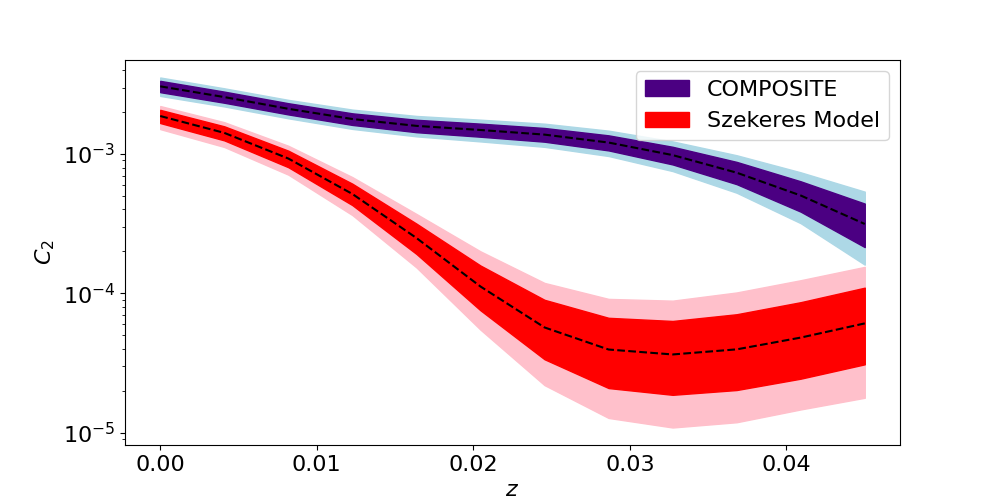
\includegraphics[width=\textwidth]{BNW Model MCMC/Special Geometry One/COMPOSITE/Hub C2.png}
        \caption{}
    \end{subfigure}
    \caption{The simulated CMB and Hubble flow anisotropy for two different observers in the geometry specified by \eqref{\ref{eqn: BNW special geometry}}. The left column (a, c, and e) shows the results for an observer fitting the CMB dipole, whereas the right column (b, d, and f) shows the results for an observer fitting the COMPOSITE Hubble flow anisotropy. The relative positions of these observers can be seen in Figure \ref{fig: special geometry density contrast}. The CMB plots in this figure is shown in the frame with the poles pointing in the radial direction, i.e., $\theta=0$ is aligned with $\partial_r$.}
    \label{fig: special geometry different observers}
\end{figure}


\section{Discussion}
In this chapter, we explored the parameter space of the BNW model to find where acceptable fits to the CMB dipole amplitude can be found, and where acceptable fits to the Hubble expansion anisotropy in the COMPOSITE catalogue can be found. We independently replicated the analysis of the canonical BNW model conducted by Hills \cite{RN42}, which corrected a bug in the original analysis by BNW. Our code used null geodesics integrated in projective coordinates as opposed to the spherical polar coordinates adopted by BNW and by Hills, and found the same CMB dipole amplitude and quadrupole power, and COMPOSITE Hubble expansion anisotropy.
Unfortunately, we could not find a set of parameters fitting both the CMB dipole and COMPOSITE Hubble expansion dipole. Within the models, the observables were significantly affected by the inhomogeneities present, but this did not allow for a noticeably better fit than a simple FLRW model with a boosted observer.

\subsection{Comparison to Observed Structure}
When fitting to the Hubble expansion anisotropy seen in the COMPOSITE catalogue, we would not expect a perfect replication of large scale structure in our surrounding region. The BNW model is far too simplistic to achieve such a feat. However, we might expect certain properties such as the size of the void or thickness of the overdensity to be similar to that seen in observed structure.

As seen in Figure \ref{fig: BNW Hubble expansion dip and quad MCMC corner}, fitting to the Hubble expansion anisotropy seen in the COMPOSITE catalogue places a tight restriction on the size of the void and radial position of the observer. The size of the void is restricted to $r_0 = 38.22^{+17.66}_{-3.28}\, h^{-1}\,$Mpc, and the observer is restricted to the edge of the void with $r_\text{obs} = 38.29^{+9.83}_{-3.25}\, h^{-1}\,$Mpc. These are both the coordinate radii, which is not an observable quantity (unlike a proper distance projected along the light cone). In fact, due to shell shifting, it can be quite different to other measures such as the proper length or luminosity distance to the centre of the void. However, $r_0$ does provide a reasonable measure for the radius of the void, as the proper distance from $r=r_0$, $\theta=0$, to $r=r_0$, $\theta=\pi$ (across the diameter of the void along the axis of symmetry) is only slightly lower than $2r_0$ for all the geometries plotted. The difference arises due to the curvature function, and as it generally falls in the range $-10^{-4} \lesssim k(r) < 0$, the difference is on the order of $0.01\%$ or less.

The size of the voids found when fitting to COMPOSITE or to the CMB dipole are consistent with the range of radii observed in void catalogues of $30\, h^{-1}\,$Mpc to $80\, h^{-1}\,$Mpc \cite{RN197}.
Notably, the range of the voids that fit to the COMPOSITE catalogue are significantly smaller than those of toy models proposed to resolve the Hubble tension, which are on the scale of hundreds of megaparsecs and have a density contrast of $\delta_\rho \sim -0.8$ \cite{RN198,RN124}.

When fitting to COMPOSITE, the observer is restricted to the edge of the void ($r_\text{obs} \approx r_0$) and in $68\%$ of the samples is restricted to $0.63\,\pi < \theta_ \text{obs} < 0.89\,\pi$, as seen in Figure \ref{fig: BNW Hubble expansion dip and quad MCMC corner}. This corresponds to the observer generally being inside or on the boundary of the overdensity located around $r=r_0$, $\theta=\pi$ -- for example, the observer position in Figures \ref{fig: BNW model best COMPOSITE fit density contrast}, \ref{fig: BNW model 0.5 quantile density contrast}, and \ref{fig: special geometry density contrast}. The observer's position inside an overdensity qualitatively matches the observations of the `Local Sheet' \cite{RN74,RN240,RN241}, a structure of galaxies including the Milky Way approximately in the shape of a flattened oblate ellipsoid \cite{RN241}. It is $0.5 - 3$ Mpc thick in the $z$ direction of the supergalactic coordinate system, and has a diameter of $\sim 10$ Mpc in the $x$ and $y$ directions of the supergalactic coordinate system \cite{RN74,RN240}. However, the observer being on the edge of the void is somewhat troubling, as the Local Group is inside a void \cite{RN74}. This observer position is also somewhat contradictory to the original aim of finding a realistic model, which sought to model more distant overdensities such as the Virgo supercluster, with the observer being located inside the void.

The overdensities in the BNW model are usually thin and long, forming curved walls, as seen in the density contrast plots thus far. To compare the thickness of these overdense structures to observations, we quantify the thickness of the overdensity as the proper length on the radial geodesic from $(r,\theta)=(r_0-\Delta r, \pi)$ to $(r, \theta)=(r_0+\Delta r, \pi)$. This is obviously not an observable quantity, but it serves well enough for a rough estimate. More details are shown in Appendix \ref{appendix: overdensity thickness}. Figure \ref{fig: BNW model overdensity thickness} shows histograms for the overdensity thickness obtained from the two MCMC processes and the range of observed thicknesses of the Local Sheet for comparison. The sample from fitting to the COMPOSITE catalogue is generally consistent with the thickness of the Local Sheet. However, when fitting to the CMB dipole, we see a large percentage of the sample above $10\, h^{-1}\,$Mpc. This may be caused by the large volume of good fits to the CMB dipole at large void sizes. We have set $\Delta r = 0.1\,r_0$, so the thickness of the overdensity in models with large voids will generally be larger than the thickness of the overdensity in models with small voids, unless one adjusts $\alpha$ to compensate.

\begin{figure}[t]
    \centering
    \begin{subfigure}{0.45\textwidth}
        \centering
        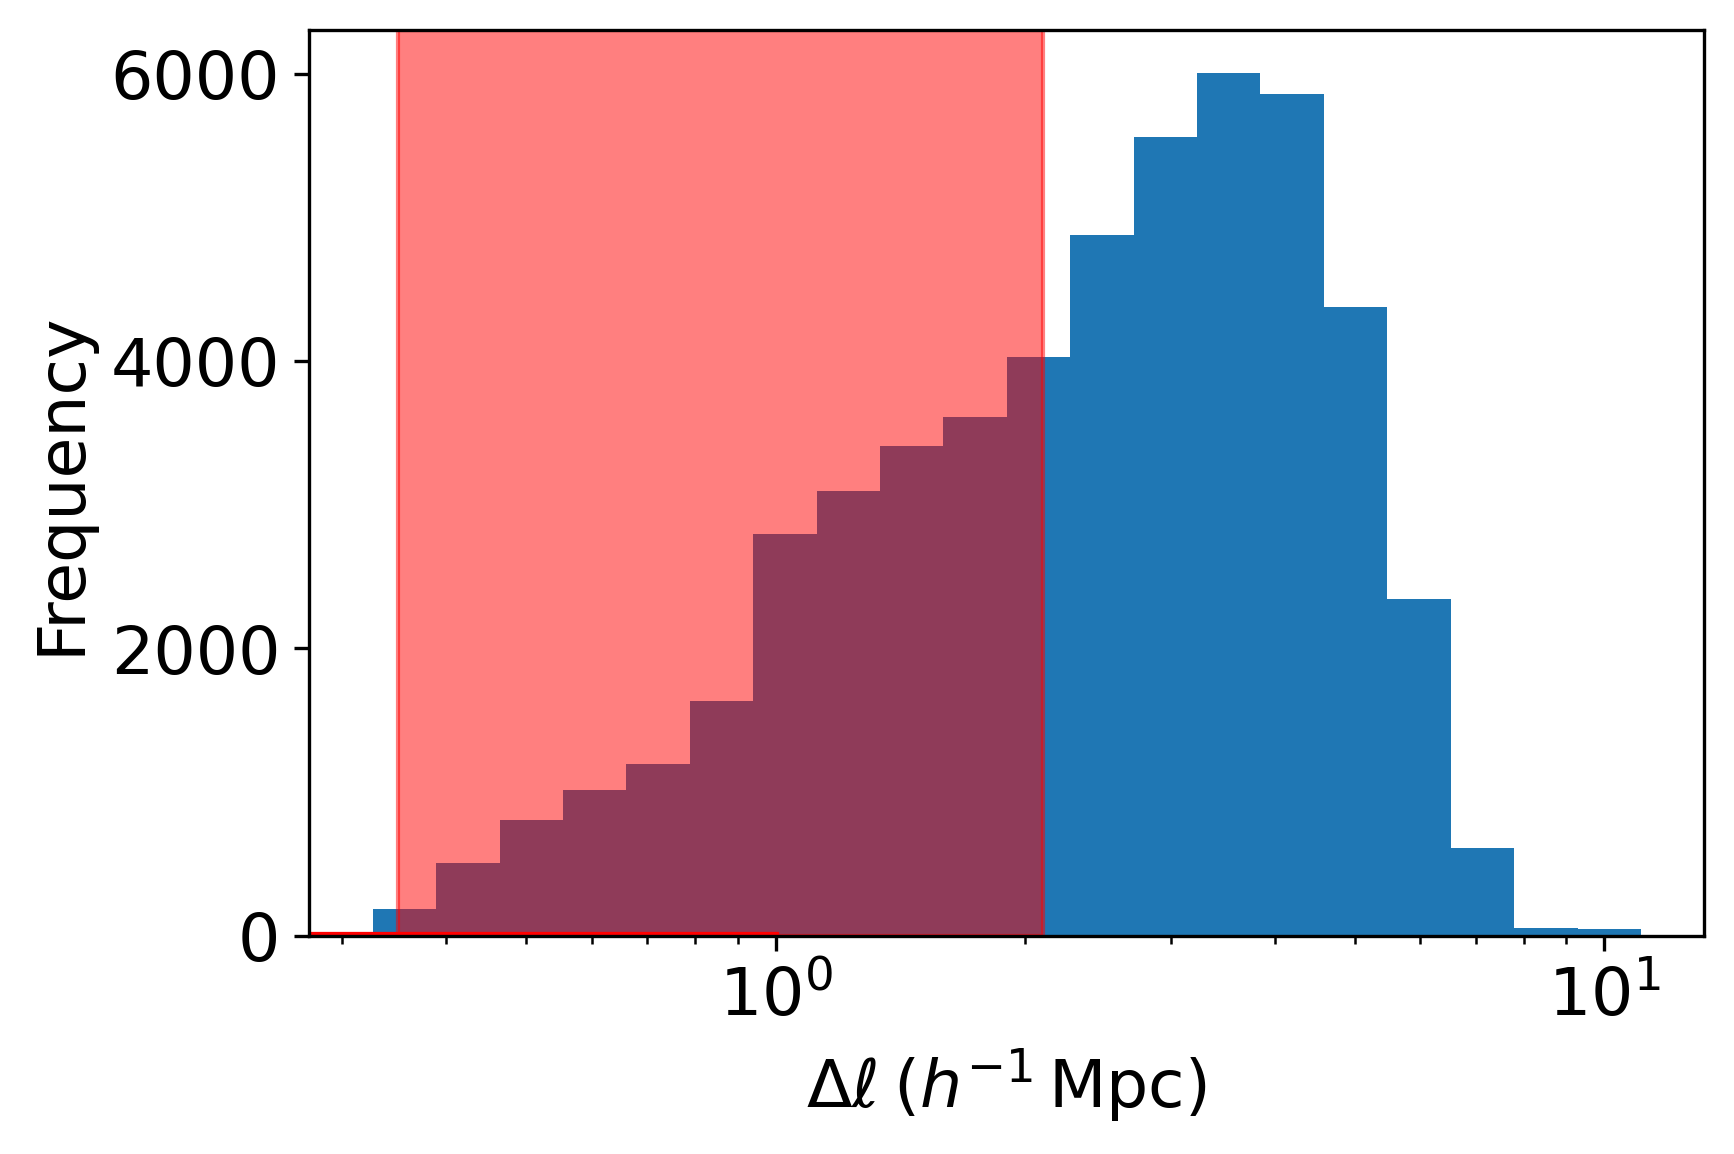
\includegraphics[width=\textwidth]{BNW Model MCMC/Distribution of overdensity thickness.png}
        \caption{}
    \end{subfigure}
    \begin{subfigure}{0.45\textwidth}
        \centering
        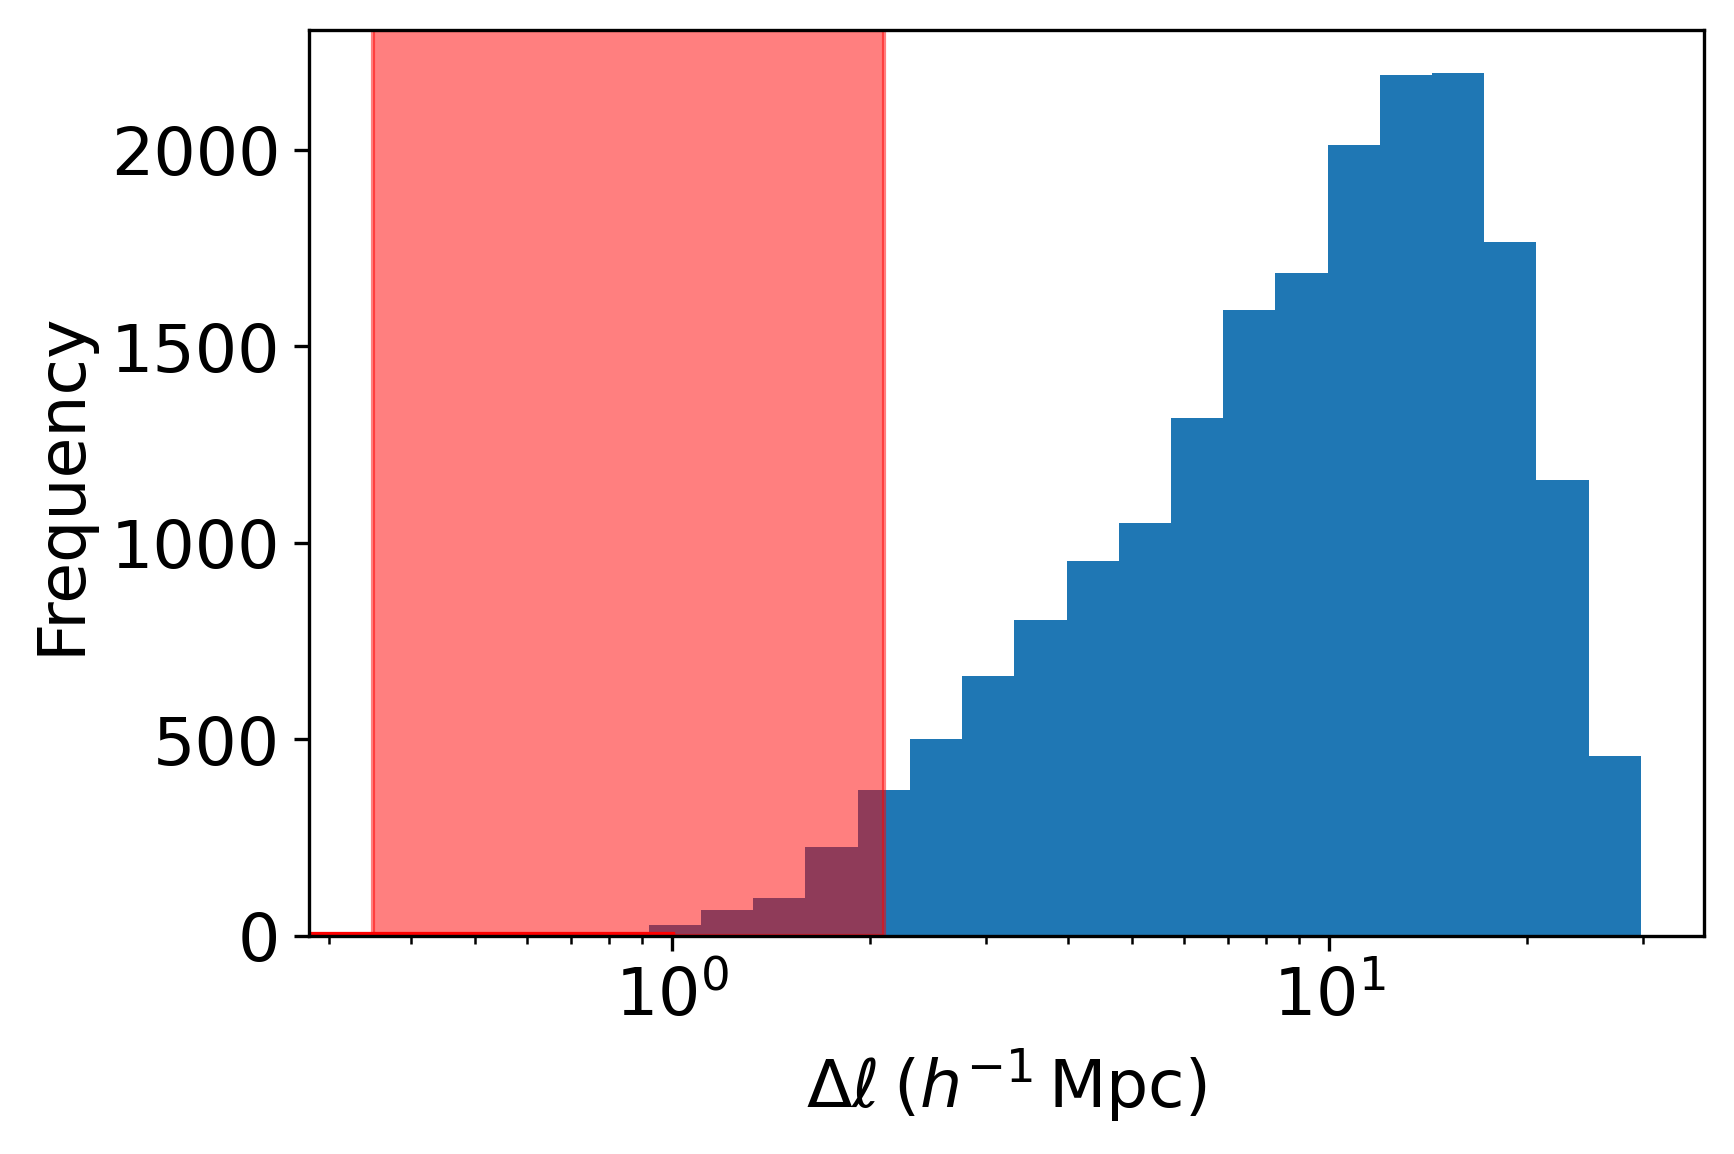
\includegraphics[width=\textwidth]{BNW Model MCMC/Distribution of overdensity thickness CMB.png}
        \caption{}
    \end{subfigure}
    \caption{Histogram of approximate overdensity thicknesses in the BNW model from: (a) fitting to COMPOSITE only, (b) fitting to the CMB dipole only. The red band shows the range of the observed thickness of the Local Sheet \cite{RN74,RN240} (using $h=0.7$ to convert from the values in the sources -- which are given in Mpc -- to $h^{-1}\,$Mpc).}
    \label{fig: BNW model overdensity thickness}
\end{figure}

\subsection{Comparison of Methodology and Results to a General Cosmographic Framework}\label{section: BNW model discussion - Asta's framework}
The methodology used in this chapter to analyse anisotropy in the Hubble flow from the COMPOSITE dataset -- outlined in Section \ref{section: introduction - hubble flow anisotropy} -- has shown itself to be useful to compare models to observation. A suitably accurate model of nearby structure should be able to replicate the observed dipole and quadrupole power of the smoothed Hubble expansion anisotropy. One downside of this approach is that the average local Hubble constant $H_0(l,b,z)$ is difficult to interpret physically. Galaxies at redshifts of $z \sim 0.01$ are below the scale of statistical homogeneity, so we would not expect the FLRW metric to apply. However, the approach we follow uses the distance-redshift Taylor expansion from the FLRW geometry with deceleration and jerk parameters inferred from CMB measurements, only quantifying inhomogeneity through the fluctuations of an average local Hubble constant. One alternative approach would be to apply a new cosmographic framework devised by Heinesen \cite{RN235}. In this formalism one finds a distance-redshift Taylor expansion for a general spacetime, where the Hubble, deceleration, jerk, and curvature parameters from the FLRW distance-redshift relation have clear analogues in functions on the observer's sky. Heinesen shows that these functions can be written in terms of a finite number of physically interpretable parameters through a spherical harmonic decomposition, with 61 degrees of freedom when the distance-redshift Taylor expansion is written up to $\mathcal{O}(z^3)$. Compared to the methodology used here, the results from Heinesen's formalism are easier to interpret physically. They may also be faster to compute for exact cosmological models, as the parameters in Heinesen's framework have exact (if complicated) mathematical representations. Thus, luminosity distances for nearby sources can be calculated without applying computationally expensive ray tracing. Such work is in progress \cite{RN261}. Although, as it is a Taylor series, the analytic expressions will only hold for small $z$ and cannot be applied to simulate a CMB measurement.

%% asta's stuff - density gradients
A recent paper by Macpherson and Heinesen \cite{RN238} applied Heinesen's new cosmographic framework to numerical relativity simulations of realistic structure formation with smoothing scales of $200\, h^{-1}\,$Mpc and $100\, h^{-1}\,$Mpc, much greater than the scales of interest here. Of particular interest to this thesis is their examination of the amplitude of the anisotropy in the Hubble, deceleration, jerk, and curvature functions and their dominating multipoles. Macpherson and Heinesen found that the amplitude of the anisotropies is generally uncorrelated with the density contrast at the observer's position, instead depending more on the spatial derivatives of the tensors associated with the timelike congruence of observers and sources (e.g., the dust congruence). If these results apply to the lower scale of the simulations in this thesis, it could explain why fitting to the COMPOSITE sample requires the observer to be at the edge of the void and generally near the overdensity, as these are the positions in the BNW model where the tensors associated with the dust congruence, such as its mass density, have high spatial gradients.

\subsection{Future Work}
As discussed in Section \ref{section: BNW model fitting CMB and COMPOSITE}, it seems unlikely that the BNW model can match both the CMB dipole and COMPOSITE Hubble expansion dipole well. In the next section, we will examine an extension of the BNW model with two overdense structures, with the aim of obtaining a better fit. That said, perhaps with the fitting information found in this section, the BNW model can be used to obtain a quantitative description of the nonlinear effects of inhomogeneities on observations. One could apply the cosmographic formalism of Heinesen \cite{RN235} with more ease than the more complicated model examined in the next section. This work is currently in progress \cite{RN261}. The model could also be used to simulate the Ellis-Baldwin test outlined in Section \ref{section: kinematic cosmic dipole tension}, which would show if the inhomogeneities in our region of spacetime would have a measurable effect on the observed distribution of radio galaxies and quasars that is distinguishable from the kinematic expectation.

The results of this chapter seem to show that the local gradients are important for matching the Hubble expansion anisotropy seen in the COMPOSITE catalogue. This feature is also seen in perturbation theory, and usually interpreted as a result of peculiar velocities. Perhaps a model would be one with multiple overdense structures, where the effects of local gradients and more distant structures can be accounted for. Then, by examining different cases, one can compare the effects of local gradients to the effects of more massive and distant overdense structures.



%%%%%%%%%%%%%%%%%%%%%%%%%%%%%%%%%%%%%%%%%%%%%%%%%%%%%%%%%%%%%%%%%%%%%%%%%%%%%%%%
                              %% TWO STRUCTURES %%
%%%%%%%%%%%%%%%%%%%%%%%%%%%%%%%%%%%%%%%%%%%%%%%%%%%%%%%%%%%%%%%%%%%%%%%%%%%%%%%%
\chapter{Extension to Two Overdensities}\label{chapter: two structures}
%%%%%%%%%%%%%%%%%%%%%%%%%%%%%%%%%%%%%%%%%%%%%%%%%%%%%%%%%%%%%%%%%%%%%%%%%%%%%%%%
In this chapter we will follow the suggestion made by BNW \cite{RN3} of extending the model by adding another overdensity with the aim of better representing the structure in our local region of the universe. This more detailed modelling of local structure may allow for a better fit of our Szekeres model to the CMB and to the galaxies of the COMPOSITE catalogue. The methodology for the analysis of this model is the same as done in Chapter \ref{chapter: BNW model analysis}.

\section{A Model with Two Overdensities}\label{sec: two structure model description}
To create a model consisting of a central void and two neighbouring overdensities, we will adapt the BNW model by changing the dipole functions and size of $\Delta r$. The parameters $r_0$, $\Delta r$, and $\delta_0$ carry over, and the parameters $\alpha_1$ and $\alpha_2$ will be introduced, which have a similar effect as $\alpha$ in the original BNW model. This allows easier comparison between the two different models, and for the physical interpretation of the parameters to carry over from the BNW model. The overdensities in this model will be separated by the shell $r=r_\text{cut}$. The inner overdensity is located at $r<r_\text{cut}$ and $\theta=\pi$, and the outer overdensity is located at $r>r_\text{cut}$ and $\phi=\pi$, with a free $\theta$ coordinate.

In this new model, $M(r)$, $\delta_M(r)$, $R(t_0,r)$, $t_B(r)$, and $Q(r)$ have the same form as the BNW model, with the only difference being that we now set $\Delta r = 0.2 r_0$ to give extra space for the second structure.

As $Q(r) = 0$, this model has bilateral symmetry with a symmetry plane at $\phi = \{0,\pi\}$. Since we will have $S',P' \neq 0$ in general, this model will not have axial symmetry, so we need to include $\phi_\text{obs}$ in the parameter space -- we cannot simply set $\phi_\text{obs} = 0$ as we did in Chapter \ref{chapter: BNW model analysis}. The bilateral symmetry does provide some simplification in that we can restrict our observer to one side of the symmetry plane, i.e., $\phi_\text{obs} \in [0,\pi]$, since an observer on the other side of the symmetry plane will have the same measurements as one with $\phi_\text{obs} \in [0,\pi]$. This bilateral symmetry does not significantly restrict the possible arrangements that the two overdensities can take around the void.

To set $S$ and $P$ we will apply a simplified version of the procedure used by Buckley and Schlegel in Section VII-E of \cite{RN1}, where they created anisotropies of random densities in random positions. In this chapter, we apply it to create two overdensities in controlled positions neighbouring a void. This simplified procedure is as follows:
\begin{enumerate}
    \item Partition the geometry by the radial coordinate into two intervals, $r \in [0, r_{\text{cut}})$ and $r \in [r_{\text{cut}}, \infty)$. The boundary $r=r_\text{cut}$ separates the inner and outer overdensities.

    \item Choose an axially symmetric model by setting $P_{\text{ax}}=0$, and choosing a piecewise $S_{\text{ax}} \neq 0$ which creates two overdensities: one in $r<r_{\text{cut}}$, and one in $r>r_{\text{cut}}$. The function $S_{\text{ax}}'/S_{\text{ax}}$ and its first derivative must vanish at $r=r_{\text{cut}}$ to ensure continuity and differentiability in the final geometry across $r=r_{\text{cut}}$.

    This can be understood as an implementation of the Darmois-Lanczos-Israel junction conditions \cite{RN245,RN242}. This is a method of ``cutting and pasting'' one geometry into another by satisfying certain junction conditions across the boundary, which became popular in General Relativity after the work of Israel in the 1960s \cite{RN242}. The junction conditions were first implemented in cosmology by Einstein and Strauss \cite{RN248,RN249} in the specific case of fitting a Schwarzschild geometry in an FLRW model, the so-called Swiss cheese model, which has been generalised to LTB\footnote{For example, see \cite{RN254} and references therein.} and Szekeres Swiss cheese \cite{RN252,RN142,RN141,RN253,RN7} and meatball models \cite{RN140}.

    \item Choose an angle $\Theta \in [0,\pi)$ corresponding to the position of the outer overdensity as taken at $r=r_{\text{cut}}$. We can restrict $\Theta$ to be positive because each model with a negative $\Theta$ is physically equivalent to a model with a positive $\Theta$, as shown in Appendix \ref{appendix: Theta proofs}. We then apply a Haantjes transformation to only the outer interval by applying \eqref{\ref{eqn: Haantjes tranform dipole functions}} in a piecewise manner using the parameters,
    \begin{equation}\label{eqn: two structures (D_1, D_2)}
        (D_1,\, D_2) = \left(\frac{\tan \left(\frac{\Theta}{2}\right)}{S_\text{ax} (r_\text{cut})},\: 0\right).
    \end{equation}
    We have chosen $D_2=0$ so that $Q=0$, giving a simpler model. A justification of \eqref{\ref{eqn: two structures (D_1, D_2)}} can also be found in Appendix \ref{appendix: Theta proofs}.

    We use $\Theta$ to parametrise the Haantjes transformation instead of $D_1$ because $\Theta$ has a more straightforward relation to the coordinate position of the overdensity, and it has finite bounds of $[0,\pi)$, making applying an MCMC process and interpreting the results easier.

    The transformed dipole functions are now
    \begin{align}
        S_H =
        \begin{cases}
            S_{\text{ax}} & r<r_{\text{cut}} \\
            \frac{S_{\text{ax}}}{T} & r \geq r_{\text{cut}}
        \end{cases}, \\
        P_H =
        \begin{cases}
            0 & r<r_{\text{cut}} \\
            \frac{D_1 S_{\text{ax}}^2}{T} & r \geq r_{\text{cut}}
        \end{cases},
    \end{align}
    where $T(r) = 1 + D_1^2 S_\text{ax}^2 (r)$.
    \item The transformed dipole functions $S_H$ and $P_H$ are not continuous at $r=r_\text{cut}$. We can resolve this by applying a scaling using \eqref{\ref{eqn: scaling dipole function transformation}} then a translation using \eqref{\ref{eqn: translation dipole function transformation}} to the outer interval only, so that for $r > r_\text{cut}$ the dipole functions are $S = \mu S_H$ and $P = \mu P_H + p_0$, where $\mu$ and $p_0$ are
    \begin{align}
        \mu &= \frac{S_{\text{ax}}(r_{\text{cut}})}{S_H(r_{\text{cut}})}, \\
        &= 1+D_1^2 S_{\text{ax}}(r_\text{cut})^2, \\
        &= T(r_\text{cut}), \\
        p_0 &= P_{\text{ax}}(r_{\text{cut}}) - \mu P_H(r_{\text{cut}}), \\
        &= 0 - T(r_\text{cut}) \frac{D_1 S_{\text{ax}}(r_{\text{cut}})^2}{T(r_\text{cut})}, \\
        &= -D_1 S_{\text{ax}}(r_{\text{cut}})^2.
    \end{align}
    Thus, the final dipole functions are
    \begin{subequations}
    \begin{align} \label{eqn: two structures transformed dipoles}
        S(r) &=
        \begin{cases}
            S_\text{ax}(r) & r < r_\text{cut} \\
            T(r_\text{cut})\frac{S_\text{ax}(r)}{T(r)}  & r \geq r_\text{cut}
        \end{cases}, \\
        P(r) &=
        \begin{cases}
            0 & r < r_\text{cut} \\
            T(r_\text{cut})\frac{D_1 S_\text{ax}^2(r)}{T(r)} - D_1 S_\text{ax}^2(r_\text{cut}) & r \geq r_\text{cut}
        \end{cases}, \\
        Q(r) &= 0.
    \end{align}
    \end{subequations}
\end{enumerate}

For the specific model used in this chapter, we modify the form chosen in Appendix D of \cite{RN1} and prescribe
\begin{equation}\label{eqn: dS over S initial}
    \frac{S'_\text{ax} (r)}{S_\text{ax}(r)} = \frac{1}{1+r}
    \begin{cases}
        \alpha_1\, b(r, r_0-2\Delta r, r_\text{cut} - \delta_r) & r < r_\text{cut} \\
        \alpha_2\, b(r, r_\text{cut} + \delta_r, r_\text{cut} + 2\Delta r) & r \geq r_\text{cut}
    \end{cases},
\end{equation}
where
\begin{equation}
    b(r,a,b) =
    \begin{cases}
        \left(1-\left(\frac{r-a}{\delta_r}\right)^2\right)^2 &
            a-\delta_r \leq r < a \\
        1 & a \leq r < b \\
        \left(1-\left(\frac{r-b}{\delta_r}\right)^2\right)^2 &
            b \leq r < b+\delta_r \\
        0 & \text{otherwise}
    \end{cases}.
\end{equation}
\eqref{\ref{eqn: dS over S initial}} can be integrated analytically to obtain $S_\text{ax}(r)$. This choice introduces three parameters, $\alpha_1$, $\alpha_2$, and $\delta_r$. The two parameters $\alpha_1$ and $\alpha_2$ modify the dipole functions to have similar effects as $\alpha$ does in the BNW model. As $\alpha_1$ increases, the inner overdensity's peak density contrast increases and the volume it takes up decreases, and $\alpha_2$ has a similar effect for the outer overdensity. The other parameter $\delta_r$ affects how sharp the edge of the overdensity is by determining the length that $S(r)$ uses to return to being constant.
The parameter $r_\text{cut}$ is introduced by the construction process. To simplify the parameter space, we set $\delta_r = 4\, h^{-1}\,$Mpc, and $r_\text{cut} = 1.05\, r_0$. Figure \ref{fig: two_structures unrotated and rotated example} shows how $\Theta$ affects the dipole functions and density contrasts. Two example models are shown, one without any rotation using $\Theta=0$, and one with an applied rotation using $\Theta = \pi/2$.

\begin{figure}[!b]
    \centering
    \begin{subfigure}[b]{0.45\textwidth}
        \centering
        \includegraphics[width=\textwidth]{two structures/unrotated/S dash over S.png}
        \caption{}
    \end{subfigure}
    \hfill
    \begin{subfigure}[b]{0.45\textwidth}
        \centering
        \includegraphics[width=\textwidth]{two structures/unrotated/density contrast.png}
        \caption{}
    \end{subfigure}
    \begin{subfigure}[b]{0.45\textwidth}
        \centering
        \includegraphics[width=\textwidth]{two structures/rotated/dipole functions.png}
        \caption{}
    \end{subfigure}
    \hfill
    \begin{subfigure}[b]{0.45\textwidth}
        \centering
        \includegraphics[width=\textwidth]{two structures/rotated/density contrast.png}
        \caption{}
    \end{subfigure}
    \caption{Two examples of the model, the top row (a and b) are for a geometry without any rotation ($\Theta = 0$), and the lower row (c and d) are for a geometry with a rotation ($\Theta = \pi/2$). Figures (a) and (c) show the dipole functions $S'/S$ and $P'/S$. Figures (b) and (d) show the density contrast on the plane of symmetry. The other parameters of the geometry in both examples are $\delta_0 = -0.9$, $\alpha_1 = \alpha_2 = 0.8$, and $r_0 = 40.0\, h^{-1}\,$Mpc.}
    \label{fig: two_structures unrotated and rotated example}
\end{figure}

\section{MCMC Results}\label{section: two_structures COMPOSITE MCMC}
For this model, we will just investigate the MCMC process applied to fitting COMPOSITE. While an MCMC process was applied to fit the model to the CMB, it was not sufficiently converged in time to include in this thesis.

Applying MCMC to fit to COMPOSITE with the probability distribution (\ref{eqn: COMPOSITE probability}) yields marginal posterior distributions seen in Figure \ref{fig: two_structures Hubble expansion dip and quad MCMC corner}.

\begin{figure}[!tb]
    \centering
    \includegraphics[width=0.9\textwidth]{two structures/COMP only MCMC/corner plot.png}
    \caption{The one-dimensional and two-dimensional marginal posterior distributions resulting from the MCMC process to fit the two structure model to the Hubble flow anisotropy dipole and quadrupole seen in the COMPOSITE catalogue.}
    \label{fig: two_structures Hubble expansion dip and quad MCMC corner}
\end{figure}

These distributions contain many of the same features as we saw when fitting the BNW model to COMPOSITE; namely, the correlation between $r_0$ and $r_\text{obs}$, and the narrow uncertainties on $r_0$ and $r_\text{obs}$.

The distributions of the new parameters also show some interesting results that seem to suggest the inner overdensity does not significantly affect the simulated COMPOSITE catalogue. The parameter $\alpha_1$ has an almost uniform distribution over all plots it is involved in, suggesting it does not significantly affect the observables. We also see a correlation between $\Theta$ and $\theta_\text{obs}$ showing that the observer tends to be near the outer overdensity. The marginal distribution of $\Theta$ and $\phi_\text{obs}$ shows that when $\Theta \sim 0$  or $\Theta \sim \pi$, $\phi_\text{obs}$ is largely unconstrained, as would be expected for a nearly axisymmetric geometry. However, when $\Theta$ takes intermediate values, $\phi_\text{obs}$ is restricted to large values near to $\phi=\pi$, which is the coordinate of the outer overdensity.

These correlations can be quantified with \textit{Pearson's correlation coefficient}, which is defined in \eqref{\ref{eqn: pearson correlation coefficient}}. A number close to 1 indicates a strong positive correlation, a number close to -1 indicates a strong negative correlation, and a number close to zero indicates no correlation. For the sample obtained from the MCMC process in this chapter to fit the model to COMPOSITE, the correlation coefficients are shown in Table \ref{tab: two_structures correlation coefficients}.

\begin{table}[!t]
    \centering
    \begin{tabular}{c|c c c c c c c c}
         & $\delta_0$ & $\alpha_1$ & $\alpha_2$ & $r_0$ & $\Theta$ & $r_\text{obs}$ & $\theta_\text{obs}$ & $\phi_\text{obs}$\\
         \hline
        $\delta_0$ & - & - & - & - & - & - & - & - \\
        $\alpha_1$ & 0.203 & - & - & - & - & - & - & - \\
        $\alpha_2$ & 0.201 & 0.050 & - & - & - & - & - & - \\
        $r_0$ & 0.879 & 0.226 & 0.235 & - & - & - & - & - \\
        $\Theta$ & -0.143 & -0.220 & -0.075 & -0.124 & - & - & - & - \\
        $r_\text{obs}$ & 0.630 & 0.170 & 0.267 & 0.884 & -0.060 & - & - & - \\
        $\theta_\text{obs}$ & 0.065 & 0.191 & 0.079 & 0.047 & -0.911 & 0.021 & - & - \\
        $\phi_\text{obs}$ & -0.198 & -0.090 & -0.057 & -0.208 & 0.374 & -0.086 & -0.285 & -
    \end{tabular}
    \caption{Pearson correlation coefficients of the MCMC sample obtained from fitting the two overdensities model to COMPOSITE. A number close to 1 indicates a strong positive correlation, a number close to -1 indicates a strong negative correlation, and a number close to zero indicates no correlation. Note the large correlation coefficients between: $\Theta$ and $\theta_\text{obs}$, $r_0$ and $r_\text{obs}$, $r_0$ and $\delta_0$, and $r_\text{obs}$ and $\delta_0$.}
    \label{tab: two_structures correlation coefficients}
\end{table}

The best fitting model in the MCMC sample had a goodness of fit as defined in \eqref{\ref{eqn: COMPOSITE probability}} of $\text{ln}(f_\text{COMPOSITE})\approx -47$ with the parameters
\begin{align}
    \begin{split} \label{eqn: two_structures best composite fit}
        \delta_0 &= -1.0, \\
        \alpha_1 &= 0.716, \\
        \alpha_2 &= 0.939, \\
        r_0 &= 35.2\, h^{-1}\, \text{Mpc}, \\
        \Theta &= 0.254, \\
        r_\text{obs} &= 37.5\, h^{-1}\, \text{Mpc}, \\
        \theta_\text{obs} &= 2.93, \\
        \phi_\text{obs} &= 3.07.
    \end{split}
\end{align}
The density contrast on the plane of symmetry for this parameter set can be seen in Figure \ref{fig: two_structures model best fit density contrast}, and the observables can be seen in Figure \ref{fig: two_structures COMP MCMC best fit observables}. Unfortunately, this shows that the model cannot fit to the Hubble flow quadrupole and dipole simultaneously.
\begin{figure}[!t]
    \centering
    \includegraphics[width=105mm]{two structures/COMP only MCMC/Best Fit/density contrast.png}
    \caption{The density contrast of the best fitting model. The cross marks the position of the observer projected onto the symmetry plane, i.e., only plotting the $X$ and $Z$ coordinates of the observer. The coordinate system used in this plot is a 3D image space $(X,Y,Z)$, with a projection method accounting for shell rotation and shifting, as outlined in Section \ref{section: szekeres - plotting}.}
    \label{fig: two_structures model best fit density contrast}
\end{figure}

\begin{figure}[p]
    \centering
    \begin{subfigure}[b]{105mm}
        \centering
        \includegraphics[width=\textwidth]{two structures/COMP only MCMC/Best Fit/CMB.png}
        \caption{}
    \end{subfigure}
    \\
    \begin{subfigure}[b]{105mm}
        \centering
        \includegraphics[width=\textwidth]{two structures/COMP only MCMC/Best Fit/Hub C1.png}
        \caption{}
    \end{subfigure}
    \hfill
    \begin{subfigure}[b]{105mm}
        \centering
        \includegraphics[width=\textwidth]{two structures/COMP only MCMC/Best Fit/Hub C2.png}
        \caption{}
    \end{subfigure}
    \caption{These plots show the simulated observables and compare the simulated COMPOSITE Hubble expansion anisotropy to the observed value. The observables plotted are, (a): the simulated CMB $\Delta T / T_0$, (b): the Hubble expansion anisotropy dipole, and (c): the Hubble expansion anisotropy quadrupole. The simulated quantities are from the model found with the maximum $f_\text{COMPOSITE}$ value, i.e., \ref{eqn: two_structures best composite fit}. The CMB has a dipole of $\Delta T = 3.14\, \si{mK}$ ($54\%$ of the observed value, at $7.3 \sigma$) and a quadrupole of $\mathcal{D}_2 = 715\, (\mu \si{K})^2$ (almost three times larger than the observed quadrupole power). The CMB in this figure is shown in the frame with the poles pointing in the radial direction, i.e., $\theta=0$ is aligned with $\partial_r$.}
    \label{fig: two_structures COMP MCMC best fit observables}
\end{figure}
\FloatBarrier

To consider a `typical' parameter fit to COMPOSITE, we examine the 0.5 quantile model (i.e., the median of each variable when considered individually), which has parameters given in the titles of Figure \ref{fig: two_structures Hubble expansion dip and quad MCMC corner}. The density contrast on the symmetry plane for this model is shown in Figure \ref{fig: two_structures 0.5 quantile density contrast.}, and the simulated observables are shown in Figure \ref{fig: two_structures COMP MCMC 0.5 quantile observables}. The simulated CMB dipole is $\Delta T = 3.17\,$mK (55\% of the observed dipole, and at $7.2 \sigma$), and the simulated quadrupole power is $7.32\, (\mu \text{K})^2$ (3\% of the observed quadrupole power).
\begin{figure}[!b]
    \centering
    \includegraphics[width=105mm]{two structures/COMP only MCMC/0.5 quantile/density contrast.png}
    \caption{The density contrast on the plane of symmetry for the model with parameters taking their median values, as shown in the titles of Figure \ref{fig: two_structures Hubble expansion dip and quad MCMC corner}. The cross marks the position of the observer projected onto the symmetry plane, i.e., only plotting the $X$ and $Z$ coordinates of the observer. The coordinate system used in this plot is a 3D image space $(X,Y,Z)$, with a projection method accounting for shell rotation and shifting, as outlined in Section \ref{section: szekeres - plotting}.}
    \label{fig: two_structures 0.5 quantile density contrast.}
\end{figure}

\begin{figure}[tb]
    \centering
    \begin{subfigure}[b]{105mm}
        \centering
        \includegraphics[width=\textwidth]{two structures/COMP only MCMC/0.5 quantile/CMB.png}
        \caption{}
    \end{subfigure}
    \\
    \begin{subfigure}[b]{105mm}
        \centering
        \includegraphics[width=\textwidth]{two structures/COMP only MCMC/0.5 quantile/Hub C1.png}
        \caption{}
    \end{subfigure}
    \hfill
    \begin{subfigure}[b]{105mm}
        \centering
        \includegraphics[width=\textwidth]{two structures/COMP only MCMC/0.5 quantile/Hub C2.png}
        \caption{}
    \end{subfigure}
    \caption{These plots show the simulated observables and compare the simulated COMPOSITE Hubble expansion anisotropy to the observed value. The observables plotted are, (a): the simulated CMB $\Delta T / T_0$, (b): the Hubble expansion anisotropy dipole, and (c): the Hubble expansion anisotropy quadrupole. The simulated quantities are from the model with the median parameters values shown in the titles of Figure \ref{fig: two_structures Hubble expansion dip and quad MCMC corner}. The CMB has a dipole of $\Delta T = 3.17\,$mK (55\% of the observed dipole, and at $7.2 \sigma$) and a quadrupole of $7.32\, (\mu \text{K})^2$ (3\% of the observed quadrupole power). The CMB in this figure is shown in the frame with the poles pointing in the radial direction, i.e., $\theta=0$ is aligned with $\partial_r$.}
    \label{fig: two_structures COMP MCMC 0.5 quantile observables}
\end{figure}

The distribution of $\alpha_1$ in Figure \ref{fig: two_structures Hubble expansion dip and quad MCMC corner} is almost flat and uncorrelated with other variables. So in Figure \ref{fig: two_structures varying alpha_1 on 0.5 quantile fit}, we examine the effect $\alpha_1$ has on the observables by varying $\alpha_1$ and showing the resultant variation of the CMB dipole, the CMB quadrupole, and $f_\text{COMPOSITE}$. The other parameters are kept constant at their median values. We see that $\alpha_1$ has very little effect on the CMB dipole and quadrupole, and only changes $f_\text{COMPOSITE}$ by 2 over its whole range.

\begin{figure}[tb]
    \centering
    \begin{subfigure}[b]{0.45\textwidth}
        \centering
        \includegraphics[width=\textwidth]{two structures/COMP only MCMC/0.5 quantile/varying alpha_1/CMB Dipole varying alpha_1.png}
        \caption{}
    \end{subfigure}
    \hfill
    \begin{subfigure}[b]{0.45\textwidth}
        \centering
        \includegraphics[width=\textwidth]{two structures/COMP only MCMC/0.5 quantile/varying alpha_1/CMB quadrupole varying alpha_1.png}
        \caption{}
    \end{subfigure}
    \\
    \begin{subfigure}[b]{0.45\textwidth}
        \centering
        \includegraphics[width=\textwidth]{two structures/COMP only MCMC/0.5 quantile/varying alpha_1/Comp lp varying alpha_1.png}
        \caption{}
    \end{subfigure}
    \caption{The variation in the simulated observables as $\alpha_1$ varies from 0 to 1. These subplots show the following observables: (a): the simulated CMB dipole, (b): the simulated CMB quadrupole, and (c): $\text{ln}(f_\text{COMPOSITE})$, the goodness of fit (less negative is a better fit). The other parameters take the median values seen in the title of Figure \ref{fig: two_structures Hubble expansion dip and quad MCMC corner}.}
    \label{fig: two_structures varying alpha_1 on 0.5 quantile fit}
\end{figure}

\section{Discussion}

\subsection{Comparison to the BNW model}
When using MCMC methods to fit the new `two overdensities model' to the dipole and quadrupole components of the Hubble expansion anisotropy in the COMPOSITE catalogue, the results maintain many of the features seen when fitting the BNW model to the COMPOSITE catalogue. We were unable to obtain a better fit to COMPOSITE with this model than we did with the BNW model. The maximum goodness of fit found when fitting to the COMPOSITE catalogue with the BNW model was $\text{ln}(f_\text{COMPOSITE}) \approx -45$, whereas when using the model with two overdensities introduced in this chapter, the maximum was only $\text{ln}(f_\text{COMPOSITE}) \approx -47$. The amplitude of the CMB dipole for the models which fit best to COMPOSITE is also not improved when compared to the BNW model. For the plotted models presented in both Chapter \ref{chapter: BNW model analysis} and in this chapter, whose simulated COMPOSITE catalogue matches the observed Hubble expansion anisotropy dipole, the simulated CMB dipole generally falls between 50\% and 55\% of the observed CMB dipole amplitude of $5.77 \pm 0.36\,$mK.

In Figure \ref{fig: two_structures Hubble expansion dip and quad MCMC corner} we saw that for a representative sample of models which fit to the dipole and quadrupole of the COMPOSITE Hubble expansion anisotropy, several of the model parameters are correlated. This is quantified in Table \ref{tab: two_structures correlation coefficients} which presents the Pearson correlation coefficient for each pair of variables. Many of the parameters of the model with two overdensities serve identical or very similar purposes to parameters of the original BNW model, and have similarly large coefficients. Namely, $\delta_0$, $r_0$, $r_\text{obs}$, and $\theta_\text{obs}$ serve a similar purpose in both models. Table \ref{tab: comparison of correlation coefficients} compares the correlation coefficients found for each model. The only strong correlation found for the two overdensities model not contained in this table is the correlation between $\Theta$ and $\theta_\text{obs}$, which has a Pearson correlation coefficient of $\rho_{\Theta,\theta_\text{obs}}=-0.911$.

\begin{table}[htb]
    \centering
    \begin{tabular}{c|c c}
         Parameters & BNW Model & Two Overdensities Model \\
         \hline
         $\delta_0, r_0$ & 0.951 & 0.879 \\
         $\delta_0, r_\text{obs}$ & 0.525 & 0.630 \\
         $\delta_0, \theta_\text{obs}$ & -0.187 & 0.065 \\
         $r_0, r_\text{obs}$ & 0.536 & 0.884 \\
         $r_0, \theta_\text{obs}$ & -0.176 & 0.047 \\
         $r_\text{obs}, \theta_\text{obs}$ & -0.204 & 0.021
    \end{tabular}
    \caption{The Pearson correlation coefficients, $\rho_{X,Y}$, obtained for the BNW model (Chapter \ref{chapter: BNW model analysis}) and the two overdensities model (Chapter \ref{chapter: two structures}) when fitting to the dipole and quadrupole components of the COMPOSITE Hubble expansion anisotropy. Only parameters present in both models with similar effects on the model are shown. A Pearson correlation coefficient close to zero indicates no correlation, and a Pearson correlation coefficient close to 1 or -1 indicates a strong positive or negative correlation. The full set of Pearson correlation coefficients for the BNW model can be found in Table \ref{tab: BNW correlation coefficients}, and the full set of Pearson correlation coefficients for the two overdensities model can be found in Table \ref{tab: two_structures correlation coefficients}.}
    \label{tab: comparison of correlation coefficients}
\end{table}

In Table \ref{tab: comparison of correlation coefficients} one can see that the two overdensities model has similar correlations to the BNW model. There are strong correlations between $\delta_0$ and $r_0$, $\delta_0$ and $r_\text{obs}$, and $r_0$ and $r_\text{obs}$. The remaining variables have very weak correlations. There are two notable differences between the two models' correlation coefficients:
\begin{enumerate}
    \item The correlation between $r_0$ and $r_\text{obs}$ is stronger in the two overdensities model.
    \item The correlations between $\theta_\text{obs}$ and the other variables are much weaker in the two overdensities model than in the BNW model.
\end{enumerate}
 The first difference indicates that the radial position of the observer is much more tightly constrained relative to the size of the void in the two overdensities model. As the observer is either inside or on the edge of the outer overdensity (as discussed later), this may suggest that the size of this outer overdensity is generally thinner than in the BNW model, despite the larger ratio between $\Delta r$ and $r_0$ used for this model. The latter difference may be caused by the variable position of the outer overdensity in the two overdensities model. In the two overdensities model the $\theta$ coordinate of the outer overdensity can vary, whereas in the BNW model, the single overdensity is fixed at $\theta=\pi$. It is not surprising that this reduces some of the dependency on the $\theta_\text{obs}$ coordinate, particularly given the correlation between $\theta_\text{obs}$ and $\Theta$, which affects the position of the outer overdensity.

\subsection{Potential Improvements to the Model}
The model investigated in this chapter contained two overdense structures. One `inner overdensity' with radial coordinate $r < r_0$, and one `outer overdensity' with radial coordinate $r > r_0$. The inner overdensity did not significantly affect the simulated CMB or COMPOSITE catalogue, as seen in Figure \ref{fig: two_structures Hubble expansion dip and quad MCMC corner} by the uniform distribution of $\alpha_1$, and in Figure \ref{fig: two_structures varying alpha_1 on 0.5 quantile fit} by the negligible dependence of the observables on $\alpha_1$. Comparatively, the parameters controlling the outer overdensity, $\Theta$ and $\alpha_2$, have a much larger effect on the distribution, as seen by the tighter constraints on these parameters in Figure \ref{fig: two_structures Hubble expansion dip and quad MCMC corner} and the correlations between them in Table \ref{tab: two_structures correlation coefficients}. In particular, $\Theta$ and $\theta_\text{obs}$ have a strong correlation with a Pearson correlation coefficient of $\rho_{\Theta, \theta_\text{obs}} = -0.911$. The inner overdensity having a negligible effect on observables could explain why the model investigated in this chapter did not perform better than the BNW model when it came to matching observations from COMPOSITE, despite the additional structure. Excluding the inner overdensity, the structures in the two overdensities model that would create anisotropy in observables are the underdense void, and the outer overdensity neighbouring the void that contains the observer. This is very reminiscent of the BNW model qualitatively.

A clear step to improve the model would be to modify the model so that the inner overdensity has a non-negligable effect on the simulated CMB and the simulated COMPOSITE catalogue. Some simple approaches to this are to:
\begin{enumerate}
    \item Adjust the ratios of $r_\text{cut}$ and $\Delta r$ to $r_0$, or the fixed value of $\delta_r$.  These parameters affect the radial position of the two overdensities and the distribution of mass between them.
    \item Choose a more suitable form of $M(r)$ more suited to a model with two overdense structures. This would give more control over the radial position of the overdensities and the distribution of mass between them.
\end{enumerate}
The first approach would be the easiest; however, it is the most limited.
The second approach would give much more control over the model, as currently the parameters of $M(r)$ ($\delta_0$, $r_0$, and $\Delta r$) are not appropriate for a model with two overdensities, since they were introduced in the BNW model to affect a model with only one overdense structure. Notably, a different choice of $M(r)$ could place an overdense structure inside the void, as was suggested in the discussion of Chapter \ref{chapter: BNW model analysis}, rather than one neighbouring it as was constructed in this chapter. A choice of $M(r)$ like that used by Bolejko and Sussman \cite{RN39} might be appropriate, however, this would increase the dimensionality of the parameter space, making finding a well fitting parameter set even more computationally expensive.

Some more difficult approaches to implement which do away with some of the assumptions of the model are:
\begin{itemize}
    \item Using an uncompensated $M(r)$. Both the BNW model and the model used in this chapter have a compensated mass, meaning the underdensity of the void is balanced out by the surrounding overdense structures so that the active gravitational mass for the outer shells is almost exactly the same as it would be for a spatially flat FLRW geometry, i.e., for shells beyond the void and overdense structures, $M(r) \approx M_0 r^3$. If we use an uncompensated $M(r)$, then there could be more or less mass in the overdensities than is needed to match the evolution of the outer shells to a spatially flat FLRW metric, i.e., for shells beyond the void and overdense structures $M(r) > M_0 r^3$ or $M(r) < M_0 r^3$. Models with an uncompensated $M(r)$ could be more difficult to implement, as the geometry and its evolution beyond the void and overdense structures will not match that of a spatially flat FLRW model. However, an uncompensated $M(r)$ would provide much more freedom in model construction. For example, one could construct a model where for $r<r_\text{cut}$ the model is exactly the same as a BNW model, giving a fully compensated void and overdensity in this inner region. Then in $r>r_\text{cut}$ we could add another overdense structure. This is not possible in the model constructed in this chapter, as it requires an uncompensated $M(r)$ to include the second overdensity. For shells further out from the origin than the second overdensity, one would have $M(r) > M_0 r^3$.

    \item Allowing for a non-uniform bang time, $t_B'(r) \neq 0$. This gives another function we can adjust to aid in constructing a model to match observations. A careful approach will be needed, as a strongly non-simultaneous bang time can lead to large inhomogeneities in the early universe which are not consistent with observations of the CMB \cite{RN258,RN259}, but a fluctuation in $t_B$ on the scale of a few hundred years can be consistent \cite{RN260}.
\end{itemize}

Compared to the simpler BNW model, the larger parameter space of the model with two overdensities introduced in this chapter extended the amount of time required to generate a suitable sample using MCMC methods. If one modifies the model in such a way that increases the number of parameters, through one of the above methods or otherwise, then the increase in dimensionality of the parameter space will further increase the computation time required. To speed up evaluation of a parameter set, one could apply the generalised anisotropic cosmographic formalism of Heinesen \cite{RN235} to the COMPOSITE catalogue and Szekeres models, as discussed previously in Section \ref{section: BNW model discussion - Asta's framework}. Such work is in progress \cite{RN261}. However, the complicated dipole functions required to model the complex inhomogeneity will make the calculations much less tractable than the BNW model, and will require extensive work with analytic computational tools first. This is also relevant for the model explored in this section, which had forms of $S$ and $P$ significantly more complicated than those in the BNW model, despite only containing one additional structure.

\clearpage
%%%%%%%%%%%%%%%%%%%%%%%%%%%%%%%%%%%%%%%%%%%%%%%%%%%%%%%%%%%%%%%%%%%%%%%%%%%%%%%%
                              %% CONCLUSION %%
%%%%%%%%%%%%%%%%%%%%%%%%%%%%%%%%%%%%%%%%%%%%%%%%%%%%%%%%%%%%%%%%%%%%%%%%%%%%%%%%
\chapter{Conclusion}\label{chapter: conclusion}
In this thesis, we have explored the potential effects of nearby large scale inhomogeneities -- such as the local void and galactic filaments -- on estimates of the CMB and galaxy catalogue measurements when the fundamental geometry governing light propagation on nearby scales, below the standard scale of statistical homogeneity, does not split simply into a background FLRW geometry and a linear perturbation. In the peculiar velocity framework commonly used with the standard $\Lambda$CDM cosmology, the dipole observed in the CMB is assumed to be purely kinematic in origin, and deviations in the redshifts of galaxies from a Hubble law are treated as the result of their motion with respect to the FLRW background. However, when considering redshift from the first principles of General Relativity, the split of redshift into a background cosmological redshift, gravitational redshift due to gravitational potentials, and Doppler redshift due to peculiar velocities is ambiguous. Perhaps it is more natural to attribute the deviation from a Hubble law to a variation in the expansion rate and its gradient across different regions of space, as caused by inhomogeneities. Given observational challenges such as the Hubble tension, anomalously large bulk flows, and the cosmic dipole tension observed in radio galaxies and quasars, it may be worth reinterpreting observational results from this perspective.

We performed our investigation using Szekeres models \cite{RN20,RN19}, an exact inhomogeneous family of solutions to Einstein's equations containing only a pressureless, comoving, irrotational dust in their energy momentum tensor. This is applied on an intermediate scale of tens of megaparsecs -- large enough where the density fluctuations within galaxies and galaxy clusters can be averaged over, but small enough that inhomogeneities are present from cosmic voids and filaments. Following the method of Bolejko, Nazer, and Wiltshire \cite{RN3} (BNW), we place a comoving observer within the Szekeres model and perform ray tracing to create estimates of the measured CMB temperature and COMPOSITE galaxy catalogue \cite{RN82,RN183}. We then compare the dipole and quadrupole components of the simulated CMB and the dipole and quadrupole power of the local average Hubble expansion anisotropy inferred from the simulated COMPOSITE catalogues to their corresponding observed quantities. The Hubble flow anisotropy dipole and quadrupole are compared at several redshifts ranging from $z=0$ to $z=0.045$, which is the range in which these large angle anisotropies in the COMPOSITE catalogue are statistically significant \cite{RN3}. It has been observed that the Local Group frame is a frame of minimum average non-linear Hubble expansion variation \cite{RN35,RN40}, i.e., the frame in which the observed distance-redshift relation when averaged in redshift bins has the least variation over the bins. Thus, assuming there is no large scale bulk flow, the simulated measurements from the model's comoving observer are compared to observations transformed to the Local Group frame. An important caveat of this choice is that the minimum average non-linear Hubble expansion variation observed in the Local Group frame can alternatively be explained by the presence of a bulk flow \cite{RN122}.

In Chapter \ref{chapter: BNW model analysis}, we performed analysis of the BNW model \cite{RN3}. This is a toy model of our region of space, consisting of a void with a neighbouring overdense region. When finding model parameters consistent with observations, we would expect the Local Group to be contained inside the void \cite{RN74}, with the overdense region modelling the Great Attractor or some other large, distant, and overdense region, such as those seen in CosmicFlows-3 \cite{RN168}. Away from this structure, the geometry is asymptotically FLRW, so as to only model the effects of structure around the observer rather than extremely large voids or other inhomogeneities on the scale of hundreds or thousands of megaparsecs. The simulations in this model and other models in this thesis used code developed independently to the code used by BNW \cite{RN3}, Dam \cite{RN6}, and Hills \cite{RN42}. Instead of the spherical coordinates used in the cited sources, our code performed ray tracing in projective coordinates. Our results for the canonical BNW model are consistent with those of Dam \cite{RN6} and Hills \cite{RN42}, showing that the original parameter set found by BNW is not consistent with the Hubble expansion anisotropy dipole inferred from the COMPOSITE catalogue. We then applied an MCMC method twice to the BNW model: once to only fit the model's parameters to the CMB dipole, which found a large volume of state space with a consistent dipole amplitude; and once to only fit the model's parameters to the Hubble expansion anisotropy dipole and quadrupole inferred from the COMPOSITE catalogue, which found much tighter bounds in general. In particular, we found that the best fits to the Hubble flow dipole and quadrupole were when the observer was either in or around the overdense region of the BNW model. This may be due to a strong dependence of the simulated observables on spatial gradients of the dust congruence tensors at the observer, as was found to be the case in numerical relativity simulations conducted on much larger scales \cite{RN238}, and as is the case in perturbation theory in the standard cosmological model. The parameter sets with the greatest likelihood function, $f_\text{COMPOSITE}$, were also somewhat grouped around a void radius of $38.22^{+17.66}_{-3.28}\, h^{-1}\,$Mpc, though reasonable fits could be found at larger void radii. Unfortunately, we were unable to find a parameter set which satisfactorily fit both the CMB dipole and the large angle anisotropies of the COMPOSITE catalogue. Generally, the simulated CMB dipole amplitude was only 50\% to 58\% of the observed CMB dipole of $5.77 \pm 0.36\,$mK for the plotted geometries which fit to the COMPOSITE catalogue. However, we were able to find geometries where an observer in one location would observe a consistent CMB, and an observer in another location would observe a Hubble expansion anisotropy dipole consistent with the COMPOSITE catalogue.

In Chapter \ref{chapter: two structures} we modified the BNW model to include a second overdense region with the aim of better modelling large scale structure in our region of space. This model also failed to simultaneously fit the dipole and quadrupole of the Hubble expansion anisotropy inferred from the COMPOSITE catalogue. However, our results showed that the shape and density contrast of the inner overdensity (controlled by the parameter $\alpha_1$) did not have a significant effect on the simulated CMB and Hubble flow anisotropies. Additionally, when fitting to the COMPOSITE catalogue the observer's position was correlated with the position of the outer overdensity -- the Pearson correlation coefficient of the observer's $\theta_\text{obs}$ coordinate and the amount the overdensity is rotated, $\Theta$, is $\rho_{\Theta,\theta_\text{obs}} = -0.911$, which suggests a strong linear correlation. From this, we can conclude that the Hubble expansion dipole and quadrupole is much more strongly affected by the outer overdensity than the inner overdensity. Any further investigations with this model may have to adjust it to make the inner overdensity have a more significant effect, perhaps by exploring different values of the fixed parameters $r_\text{cut}$, $\Delta r$, and $\delta_r$, or by choosing a new form of $M(r)$ to distribute the mass differently. One could also apply different approaches to model construction such as the `q-scalar' approach \cite{RN30,RN41,RN60}, which is thought to be more computationally efficient, and may provide a more intuitive approach to model construction than the methods used in this thesis. The correlation between the observer's position and the position of the outer overdensity is similar to the results of the observer in the BNW model being constrained to in and around the overdensity. This seconds the hypothesis of the simulated large angle anisotropies in observations having a significant dependence on the spatial gradients at the observer's position.

Overall, the models examined in this thesis do not achieve much more than a simple FLRW model with a boosted observer in regard to the investigated observations. They cannot match the CMB dipole and quadrupole, and the large angle Hubble expansion anisotropies simultaneously. And, they cannot match both the dipole and quadrupole power of the Hubble expansion anisotropy inferred from the COMPOSITE catalogue. While it is possible that a more complicated model could succeed where the models in this thesis have failed, complex models will have large parameter spaces that quickly become computationally expensive to explore as their dimensionality increases. Perhaps other approaches, such as Heinesen's generalised anisotropic cosmographic formalism \cite{RN235,RN238,RN236}, are more appropriate.

These models were originally intended to simulate the effects of distant overdensities such as the Great Attractor, which neighbour the local void. However, once MCMC methods were applied, we found that the COMPOSITE catalogue constrained the observer to be in or around the overdense region neighbouring the void, rather than inside the void as one might expect. Perhaps further investigations could include an overdense region inside the void at the observer's position, and a second larger overdense region further out. This could more closely match observations of local structure by including a nearby structure such as the Local Sheet \cite{RN74,RN240,RN241} inside the void and a distant overdense region like the Great Attractor \cite{RN168}, whilst maintaining the sharp local gradients that may have a dominating effect on large angle anisotropies. By adjusting the parameters affecting the distant overdense region independently to those affecting the overdense region containing the observer, one could examine the relative dependence of observations on these structures, and test the hypothesis of dependence on local gradients. However, the Szekeres models are ultimately limited in what they can model. The dust must be irrotational, the density is limited to be dipole-like on each shell of constant $r$, and we cannot have structure which evolves in such a way that create shell crossings. This last limitation is particularly significant, as it constrains the modelling power of collapsing structures. These limitations may prevent the Szekeres models from creating a suitable model, despite its relative generality compared to other exact solutions to Einstein's equations.

If a suitable model can be found, different observations can be simulated to examine the effect of inhomogeneities on various observational challenges. These could include, for example, simulating catalogues from which anomalously large bulk flows are inferred, or simulating an Ellis-Baldwin test \cite{RN67} such as the recent one performed with quasars by Secrest \etal \cite{RN31,RN167}. The results from such a simulation could be compared to observations to test if non-kinematic effects caused by inhomogeneities on this scale have a measurable effect on these tensions.

\cleardoublepage
\phantomsection
\addcontentsline{toc}{chapter}{Bibliography}
\printbibliography



%%%%%%%%%%%%%%%%%%%%%%%%%%%%%%%%%%%%%%%%%%%%%%%%%%%%%%%%%%%%%%%%%%%%%%%%%%%%%%%%
                              %% APPENDIX %%
%%%%%%%%%%%%%%%%%%%%%%%%%%%%%%%%%%%%%%%%%%%%%%%%%%%%%%%%%%%%%%%%%%%%%%%%%%%%%%%%
\begin{appendices}

%% Proof of k(r) <= 0
\chapter{Proof of \texorpdfstring{$k(r) \leq 0$}{non-positive curvature function}} \label{appendix: k <= 0 proof}
In a Szekeres model, the bang time $t_B(r)$ for the shell of radius $r$ is given by
\begin{equation}
    t_0 - t_B(r) = \int_0^{R(t_0,r)} \frac{\diff{\tilde{R}}}{\sqrt{\frac{2M(r)}{\tilde{R}} - k(r) + \frac{\Lambda \tilde{R}^2}{3}}}.
\end{equation}
For both the BNW model and the two structure model we choose $R(t_0,r)=r$, $t_B(r) = 0$, and $M(r)=M_0 r^3[1+\delta_M(r)]$, with $M_0$ corresponding to the asymptotic FLRW mass density so that
\begin{equation}
    t_0 = \int_0^r \frac{\diff{\tilde{R}}}{\sqrt{\frac{2M_0 r^3}{\tilde{R}} + \frac{\Lambda \tilde{R}^2}{3}}},
\end{equation}
as per a pressureless FLRW geometry.

For the sake of contradiction, let us assume that $k(r) > 0$, then
\begin{align}
    \sqrt{\frac{2M(r)}{\tilde{R}} - k(r) + \frac{\Lambda \tilde{R}^2}{3}} &<
        \sqrt{\frac{2M(r)}{\tilde{R}} + \frac{\Lambda \tilde{R}^2}{3}} \\
        &\leq \sqrt{\frac{2M_0 r^3}{\tilde{R}} + \frac{\Lambda \tilde{R}^2}{3}},
\end{align}
where we have used $M(r)=M_0 r^3[1+\delta_M(r)] \leq M_0 r^3$, which is only the case when $\delta_0 \leq 0$ (for either model). Integrating the reciprocal of both sides gives
\begin{equation}
    t_0 - t_B(r) = \int_0^r \frac{\diff{\tilde{R}}}{\sqrt{\frac{2M(r)}{\tilde{R}} - k(r) + \frac{\Lambda \tilde{R}^2}{3}}} > \int_0^r \frac{\diff{\tilde{R}}}{\sqrt{\frac{2M_0 r^3}{\tilde{R}} + \frac{\Lambda \tilde{R}^2}{3}}} = t_0.
\end{equation}
So assuming $k(r)>0$ gives $t_0 - t_B(r) > t_0 \Longrightarrow t_B(r) < 0$, however this is in clear contradiction with $t_B(r)=0$. So we can conclude that when $\delta_0 < 0$ we must have $k(r) < 0$; i.e., the presence of the void forces the spatial curvature to be negative.


%% Details of Theta
\chapter{Details of \texorpdfstring{$\Theta$}{the Haantjes rotation in the two structure model}} \label{appendix: Theta proofs}

In Section \ref{sec: two structure model description} we introduced a parameter $\Theta$ that determined the parameter $D_1$ used in the piecewise Haantjes transformation. Here we justify the use of $\Theta$ by showing its relation to the position of the outer overdensity, and we justify the restriction of $0 \leq \Theta \leq \pi$ by showing that each two structure model with $\Theta < 0$ is physically equivalent to one with $\Theta > 0$.

Applying MCMC is more straightforward if each parameter of the model falls in an interval $(a,b)$. The parameter $D_1$ used in the Haantjes transformation can take any real value, so is not convenient. Thus, here we will define a new parameter $\Theta$ to parameterise the Haantjes transformation. To make this parameter easy to physically understand, we will relate it to the spherical polar coordinates of the outer overdensity on shells just outside $r=r_\text{cut}$.

Initially, both inner and outer overdensities are located at $(p_\text{ax}, q_\text{ax}) = (0,0)$. The subscript `ax' denotes the coordinates in the untransformed axially symmetric geometry. In Section \ref{sec: two structure model description}, we perform a piecewise Haantjes transformation with arbitrary $D_1$ and $D_2=0$, then a piecewise scaling with $\mu=1+D_1^2 S_\text{ax}^2(r_\text{cut})$, and finally a piecewise translation with $(p_0, q_0)=(0,-D_1 S_\text{ax}^2(r_\text{cut})$ to rotate the outer overdensity to an arbitrary without modifying the position of the inner overdensity. All of these piecewise coordinate transformation are only applied to $r>r_\text{cut}$. Following the projective coordinates of the outer ($r > r_\text{cut}$) overdenisty through this series of transformations,
\begin{align}
    (p_\text{ax}, q_\text{ax}) &= (0,0), \\
    \Longrightarrow (p_\text{H}, q_\text{H}) &= (0,0), \\
    \Longrightarrow (p, q) &= (p_0, 0), \\
    &= (-D_1 S_\text{ax}^2 (r_\text{cut}), 0),
\end{align}
where subscript `$H$' denotes the coordinates after only the piecewise Haantjes transform, and $(p, q)$ are the projective coordinates of the overdensity in the final geometry after the scaling and translation.

Substituting these new coordinates in to \eqref{\ref{eqn: Szekeres - spherical coordinate transformation}} to transform to spherical polar coordinates,
\begin{align}
    -D_1 S_\text{ax}^2 (r_\text{cut})-P(r) &= S(r) \cot \left(\frac{\theta(r)}{2}\right) \cos(\phi(r)) \label{eqn: density extrema transform 1}\\
    0-Q(r) &= S(r) \cot \left(\frac{\theta(r)}{2}\right) \sin(\phi(r)) \label{eqn: density extrema transform 2}.
\end{align}
Here $\theta(r)$ and $\phi(r)$ are the spherical polar coordinates of the outer overdensity in the final geometry which are only defined for $r>r_\text{cut}$ (since the density is uniform on the $r=r_\text{cut}$ shell), and $S$, $P$, and $Q$ are the dipole functions in the final geometry. Substituting $Q(r)=0$ into \eqref{\ref{eqn: density extrema transform 2}} and noting that $S(r) \neq 0$ for $r>r_\text{cut}$, and assuming that $\theta(r) \neq 0, \pi$, we must have
\begin{equation}
    \sin (\phi(r)) = 0
\end{equation}
so, $\phi(r) = 0$ or $\phi(r) = \pi$. Thus, \eqref{\ref{eqn: density extrema transform 1}} becomes
\begin{align}
    -D_1 S_\text{ax}^2 (r_\text{cut})-P(r) &= \pm S(r) \cot \left(\frac{\theta(r)}{2}\right) \label{eqn: theta(r) partway}.
\end{align}
The function $\theta(r)$ is not defined when $r=r_\text{cut}$, since the density is uniform on this shell. So we instead take the limit of \eqref{\ref{eqn: theta(r) partway}} as $r \to r_\text{cut}$, as $P(r_\text{cut})=0$ and $S(r_\text{cut})=S_\text{ax}(r_\text{cut})$,
\begin{align}
    -D_1 S_\text{ax}^2 (r_\text{cut}) &= \pm S_\text{ax}(r_\text{cut}) \cot \left(\frac{\lim_{r\to r_\text{cut}}\theta(r)}{2}\right) \\
    \Longrightarrow D_1 &= \mp \frac{\cot \left(\frac{\lim_{r\to r_\text{cut}}\theta(r)}{2}\right)}{S_\text{ax}(r_\text{cut})}
\end{align}

We now define $\Theta \in (-\pi, \pi]$ as a way of parametrizing the piecewise Haantjes transformation so that
\begin{equation}\label{eqn: Theta D_1 relation appendix}
    D_1 = \frac{\cot \left(\frac{\pi - \Theta}{2}\right)}{S_\text{ax} (r_\text{cut})} = \frac{\tan \left(\frac{\Theta}{2}\right)}{S_\text{ax} (r_\text{cut})}.
\end{equation}
From this definition, one can show that $\lim_{r\to r_\text{cut}}\theta(r) = \pi - |\Theta|$, and $\phi(r) = \pi$ when $\Theta>0$ and $\phi(r)=0$ when $\Theta<0$.

Now we will show that every two structure model from Chapter \ref{chapter: two structures} with $\Theta < 0$ is physically equivalent to a two structure model with $\Theta > 0$.

For the two structure model we have $S>0$, so by \eqref{\ref{eqn: Theta D_1 relation appendix}} the sign of $D_1$ and $\Theta$ are the same, so for a model with $\Theta < 0$, $D_1 < 0$. The dipole functions for the two structure model are
\begin{subequations}
    \begin{align} \label{eqn: two structures transformed dipoles appendix}
        S(r) &=
        \begin{cases}
            S_\text{ax}(r) & r < r_\text{cut} \\
            T(r_\text{cut})\frac{S_\text{ax}(r)}{T(r)}  & r \geq r_\text{cut}
        \end{cases}, \\
        P(r) &=
        \begin{cases}
            0 & r < r_\text{cut} \\
            T(r_\text{cut})\frac{D_1 S_\text{ax}^2(r)}{T(r)} - D_1 S_\text{ax}^2(r_\text{cut}) & r \geq r_\text{cut}
        \end{cases},\label{eqn: two structures final dipoles P appendix} \\
        Q(r) &= 0.
    \end{align}
\end{subequations}
Perform a polar rotation with angle $\psi = \pi$ using \eqref{\ref{eqn: polar rotation dipole functions}}, the new dipole functions are $\tilde{S} = S$, $\tilde{P} = -P$, and $\tilde{Q} = -Q$. In full, the transformed dipole functions are,
\begin{subequations}
    \begin{align}
        \tilde{S}(r) &=
        \begin{cases}
            S_\text{ax}(r) & r < r_\text{cut} \\
            T(r_\text{cut})\frac{S_\text{ax}(r)}{T(r)}  & r \geq r_\text{cut}
        \end{cases}, \\
        \tilde{P}(r) &=
        \begin{cases}
            0 & r < r_\text{cut} \\
            -T(r_\text{cut})\frac{D_1 S_\text{ax}^2(r)}{T(r)} + D_1 S_\text{ax}^2(r_\text{cut}) & r \geq r_\text{cut}
        \end{cases}, \\
        \tilde{Q}(r) &= 0.
    \end{align}
\end{subequations}
This can be rewritten as
\begin{subequations}
    \begin{align}\label{eqn: two structures dipole functions polar rotation for negative Theta}
        \tilde{S}(r) &=
        \begin{cases}
            S_\text{ax}(r) & r < r_\text{cut} \\
            \tilde{T}(r_\text{cut})\frac{S_\text{ax}(r)}{\tilde{T}(r)}  & r \geq r_\text{cut}
        \end{cases}, \\
        \tilde{P}(r) &=
        \begin{cases}
            0 & r < r_\text{cut} \\
            \tilde{T}(r_\text{cut})\frac{\tilde{D}_1 S_\text{ax}^2(r)}{\tilde{T}(r)} - \tilde{D}_1 S_\text{ax}^2(r_\text{cut}) & r \geq r_\text{cut}
        \end{cases}, \\
        \tilde{Q}(r) &= 0,
    \end{align}
\end{subequations}
where $\tilde{D}_1 = -D_1$, and $\tilde{T}(r) = 1 + (-D_1)^2 S_\text{ax}^2 (r) = 1 + D_1^2 S_\text{ax}^2 (r) = T(r)$. \eqref{\ref{eqn: two structures dipole functions polar rotation for negative Theta}} is the same form as \eqref{\ref{eqn: two structures transformed dipoles appendix}}, so it is a two structure model with a piecewise Haantjes transformation parameter of $\tilde{D_1}$.

Thus, if we have a model where $\Theta < 0$, then it also has $D_1 < 0$, and under a polar rotation can be transformed to a model with $\tilde{D}_1 = -D_1 > 0$, so has $\tilde{\theta}_H > 0$. A polar rotation is a coordinate transformation, so these geometries are physically equivalent. So we have proven that a two structure model of Chapter \ref{chapter: two structures} with $\Theta < 0$ is physically equivalent to a two structure model with $\Theta > 0$.


%% Thickness of over-densities
\chapter{Thickness of Over-Densities}\label{appendix: overdensity thickness}
Over-densities in Szekeres models are typically long and thin (e.g., Figure \ref{fig: BNW params density contrast}). We quantify the thickness of an overdensity using the proper distance along the line of maximum density on each shell, using the radial constant coordinate time geodesic along the axis of symmetry in the BNW model and untransformed two structure model.

The proper distance between two comoving points on a purely radial geodesic from $r=a$ to $r=b$ at a constant $\theta$ is
\begin{equation}
    \Delta \ell (t) = \int_a^b \frac{R'-R\frac{\mathcal{E}'}{\mathcal{E}}}{\sqrt{1-k}} \diff{r},
\end{equation}
at the present time, $R(t_0,r)=r$ so this simplifies to
\begin{equation}
    \Delta \ell (t_0) = \int_a^b \frac{1-r\frac{\mathcal{E}'}{\mathcal{E}}}{\sqrt{1-k}}\diff{r}.
\end{equation}
We found in Section \ref{section: szekeres - plotting} that $k(r)$ is small enough to be negligible, so this further simplifies to
\begin{equation}
    \Delta \ell (t_0) = \int_a^b \left(1-r\frac{\mathcal{E}'}{\mathcal{E}}\right) \diff{r}.
\end{equation}
Below we will simplify this for the BNW explored in Chapter \ref{chapter: BNW model analysis},

\section{BNW Model}
In the BNW model, we say the overdensity starts at $r=r_0-\Delta r$ and ends at $r=r_0+\Delta_r$ along the line $\theta=\pi,\: \phi=0$. Along this radial path $\mathcal{E}'/\mathcal{E} = \alpha/r$, so,
\begin{align}
    \Delta \ell (t_0) &= \int_{r_0-\Delta r}^{r_0+\Delta r} \left(1-r\frac{\alpha}{r}\right) \diff{r}, \\
    &= \int_{r_0-\Delta r}^{r_0+\Delta r} \left(1-\alpha\right) \diff{r}. \\
    &= 2 \Delta r \left(1-\alpha\right). \label{eqn: BNW Model thickness of overdensity back of the envelope}
\end{align}

Using data obtained from the MCMC processes in Chapter \ref{chapter: BNW model analysis} we obtain the histograms of overdensity thickness seen in Figure \ref{fig: BNW model overdensity thickness appendix}.
\begin{figure}[t]
    \centering
    \begin{subfigure}{0.45\textwidth}
        \centering
        \includegraphics[width=\textwidth]{BNW Model MCMC/Distribution of overdensity thickness.png}
        \caption{}
    \end{subfigure}
    \begin{subfigure}{0.45\textwidth}
        \centering
        \includegraphics[width=\textwidth]{BNW Model MCMC/Distribution of overdensity thickness CMB.png}
        \caption{}
    \end{subfigure}
    \caption{Histogram of approximate overdensity thickness in the BNW model from (a) fitting to COMPOSITE only, (b) fitting to the CMB only. The red band shows the range of observed values for the thickness of the Local Sheet \cite{RN74,RN240}.}
    \label{fig: BNW model overdensity thickness appendix}
\end{figure}

\end{appendices}


\end{document}
